% Options for packages loaded elsewhere
\PassOptionsToPackage{unicode}{hyperref}
\PassOptionsToPackage{hyphens}{url}
%
\documentclass[
]{book}
\usepackage{lmodern}
\usepackage{amssymb,amsmath}
\usepackage{ifxetex,ifluatex}
\ifnum 0\ifxetex 1\fi\ifluatex 1\fi=0 % if pdftex
  \usepackage[T1]{fontenc}
  \usepackage[utf8]{inputenc}
  \usepackage{textcomp} % provide euro and other symbols
\else % if luatex or xetex
  \usepackage{unicode-math}
  \defaultfontfeatures{Scale=MatchLowercase}
  \defaultfontfeatures[\rmfamily]{Ligatures=TeX,Scale=1}
\fi
% Use upquote if available, for straight quotes in verbatim environments
\IfFileExists{upquote.sty}{\usepackage{upquote}}{}
\IfFileExists{microtype.sty}{% use microtype if available
  \usepackage[]{microtype}
  \UseMicrotypeSet[protrusion]{basicmath} % disable protrusion for tt fonts
}{}
\makeatletter
\@ifundefined{KOMAClassName}{% if non-KOMA class
  \IfFileExists{parskip.sty}{%
    \usepackage{parskip}
  }{% else
    \setlength{\parindent}{0pt}
    \setlength{\parskip}{6pt plus 2pt minus 1pt}}
}{% if KOMA class
  \KOMAoptions{parskip=half}}
\makeatother
\usepackage{xcolor}
\IfFileExists{xurl.sty}{\usepackage{xurl}}{} % add URL line breaks if available
\IfFileExists{bookmark.sty}{\usepackage{bookmark}}{\usepackage{hyperref}}
\hypersetup{
  pdftitle={Quantifying Life},
  pdfauthor={Dmitry Kondrashov},
  hidelinks,
  pdfcreator={LaTeX via pandoc}}
\urlstyle{same} % disable monospaced font for URLs
\usepackage{color}
\usepackage{fancyvrb}
\newcommand{\VerbBar}{|}
\newcommand{\VERB}{\Verb[commandchars=\\\{\}]}
\DefineVerbatimEnvironment{Highlighting}{Verbatim}{commandchars=\\\{\}}
% Add ',fontsize=\small' for more characters per line
\usepackage{framed}
\definecolor{shadecolor}{RGB}{248,248,248}
\newenvironment{Shaded}{\begin{snugshade}}{\end{snugshade}}
\newcommand{\AlertTok}[1]{\textcolor[rgb]{0.94,0.16,0.16}{#1}}
\newcommand{\AnnotationTok}[1]{\textcolor[rgb]{0.56,0.35,0.01}{\textbf{\textit{#1}}}}
\newcommand{\AttributeTok}[1]{\textcolor[rgb]{0.77,0.63,0.00}{#1}}
\newcommand{\BaseNTok}[1]{\textcolor[rgb]{0.00,0.00,0.81}{#1}}
\newcommand{\BuiltInTok}[1]{#1}
\newcommand{\CharTok}[1]{\textcolor[rgb]{0.31,0.60,0.02}{#1}}
\newcommand{\CommentTok}[1]{\textcolor[rgb]{0.56,0.35,0.01}{\textit{#1}}}
\newcommand{\CommentVarTok}[1]{\textcolor[rgb]{0.56,0.35,0.01}{\textbf{\textit{#1}}}}
\newcommand{\ConstantTok}[1]{\textcolor[rgb]{0.00,0.00,0.00}{#1}}
\newcommand{\ControlFlowTok}[1]{\textcolor[rgb]{0.13,0.29,0.53}{\textbf{#1}}}
\newcommand{\DataTypeTok}[1]{\textcolor[rgb]{0.13,0.29,0.53}{#1}}
\newcommand{\DecValTok}[1]{\textcolor[rgb]{0.00,0.00,0.81}{#1}}
\newcommand{\DocumentationTok}[1]{\textcolor[rgb]{0.56,0.35,0.01}{\textbf{\textit{#1}}}}
\newcommand{\ErrorTok}[1]{\textcolor[rgb]{0.64,0.00,0.00}{\textbf{#1}}}
\newcommand{\ExtensionTok}[1]{#1}
\newcommand{\FloatTok}[1]{\textcolor[rgb]{0.00,0.00,0.81}{#1}}
\newcommand{\FunctionTok}[1]{\textcolor[rgb]{0.00,0.00,0.00}{#1}}
\newcommand{\ImportTok}[1]{#1}
\newcommand{\InformationTok}[1]{\textcolor[rgb]{0.56,0.35,0.01}{\textbf{\textit{#1}}}}
\newcommand{\KeywordTok}[1]{\textcolor[rgb]{0.13,0.29,0.53}{\textbf{#1}}}
\newcommand{\NormalTok}[1]{#1}
\newcommand{\OperatorTok}[1]{\textcolor[rgb]{0.81,0.36,0.00}{\textbf{#1}}}
\newcommand{\OtherTok}[1]{\textcolor[rgb]{0.56,0.35,0.01}{#1}}
\newcommand{\PreprocessorTok}[1]{\textcolor[rgb]{0.56,0.35,0.01}{\textit{#1}}}
\newcommand{\RegionMarkerTok}[1]{#1}
\newcommand{\SpecialCharTok}[1]{\textcolor[rgb]{0.00,0.00,0.00}{#1}}
\newcommand{\SpecialStringTok}[1]{\textcolor[rgb]{0.31,0.60,0.02}{#1}}
\newcommand{\StringTok}[1]{\textcolor[rgb]{0.31,0.60,0.02}{#1}}
\newcommand{\VariableTok}[1]{\textcolor[rgb]{0.00,0.00,0.00}{#1}}
\newcommand{\VerbatimStringTok}[1]{\textcolor[rgb]{0.31,0.60,0.02}{#1}}
\newcommand{\WarningTok}[1]{\textcolor[rgb]{0.56,0.35,0.01}{\textbf{\textit{#1}}}}
\usepackage{longtable,booktabs}
% Correct order of tables after \paragraph or \subparagraph
\usepackage{etoolbox}
\makeatletter
\patchcmd\longtable{\par}{\if@noskipsec\mbox{}\fi\par}{}{}
\makeatother
% Allow footnotes in longtable head/foot
\IfFileExists{footnotehyper.sty}{\usepackage{footnotehyper}}{\usepackage{footnote}}
\makesavenoteenv{longtable}
\usepackage{graphicx}
\makeatletter
\def\maxwidth{\ifdim\Gin@nat@width>\linewidth\linewidth\else\Gin@nat@width\fi}
\def\maxheight{\ifdim\Gin@nat@height>\textheight\textheight\else\Gin@nat@height\fi}
\makeatother
% Scale images if necessary, so that they will not overflow the page
% margins by default, and it is still possible to overwrite the defaults
% using explicit options in \includegraphics[width, height, ...]{}
\setkeys{Gin}{width=\maxwidth,height=\maxheight,keepaspectratio}
% Set default figure placement to htbp
\makeatletter
\def\fps@figure{htbp}
\makeatother
\setlength{\emergencystretch}{3em} % prevent overfull lines
\providecommand{\tightlist}{%
  \setlength{\itemsep}{0pt}\setlength{\parskip}{0pt}}
\setcounter{secnumdepth}{5}
\usepackage{booktabs}
\usepackage{chemarr}
\usepackage{makeidx}
\makeindex
\usepackage{chemarr}
\usepackage[]{natbib}
\bibliographystyle{apalike}

\title{Quantifying Life}
\author{Dmitry Kondrashov}
\date{2021-03-30}

\usepackage{amsthm}
\newtheorem{theorem}{Theorem}[chapter]
\newtheorem{lemma}{Lemma}[chapter]
\newtheorem{corollary}{Corollary}[chapter]
\newtheorem{proposition}{Proposition}[chapter]
\newtheorem{conjecture}{Conjecture}[chapter]
\theoremstyle{definition}
\newtheorem{definition}{Definition}[chapter]
\theoremstyle{definition}
\newtheorem{example}{Example}[chapter]
\theoremstyle{definition}
\newtheorem{exercise}{Exercise}[chapter]
\theoremstyle{remark}
\newtheorem*{remark}{Remark}
\newtheorem*{solution}{Solution}
\begin{document}
\maketitle

{
\setcounter{tocdepth}{1}
\tableofcontents
}
\hypertarget{purpose-and-purview}{%
\chapter*{Purpose and purview}\label{purpose-and-purview}}
\addcontentsline{toc}{chapter}{Purpose and purview}

\begin{quote}
What is a man, said Athos, who has no landscape? Nothing but mirrors and tides.\\
-- Anne Michaels, \textbf{Fugitive Pieces}
\end{quote}

This is an online book to help biologists and biology-adjacent folks learn quantitative skills through the practice of programming in R. These skills can be roughly sorted into four types:

\begin{itemize}
\item
  Building models and understanding assumptions
\item
  Writing code to perform computational tasks
\item
  Performing mathematical analysis of models
\item
  Working with data and using statistical tools
\end{itemize}

These skills interface, intertwine, and reinforce each other in the practice of biological research and are thus presented concurrently in this book, instead of being corralled into separate courses taught by different departments, like mathematics, statistics, and computer science. Here I combine ideas and skills from all of these disciplines into an educational narrative organized by increasing exposure to programming concepts.

\hypertarget{a-brief-motivation-of-mathematical-modeling}{%
\section{A brief motivation of mathematical modeling}\label{a-brief-motivation-of-mathematical-modeling}}

A mathematical model is a representation of some real object or phenomenon in terms of quantities (numbers). The goal of modeling is to create a description of the object in question that may be used to pose and answer questions about it, without doing hard experimental work. A good analogy for a mathematical model is a map of a geographic area: a map cannot record all of the complexity of the actual piece of land, because then the map would need to be size of the piece of land, and then it wouldn't be very useful! Maps, and mathematical models, need to sacrifice the details and provide a birds-eye view of reality in order to guide the traveler or the scientist. The representation of reality in the model must be simple enough to be useful, yet complex enough to capture the essential features of what it is trying to represent.

Mathematical modeling has long been essential in physics: for instance, it is well known that distance traveled by an object traveling at constant speed \(v\) is proportional to the time traveled (called \(t\)). This mathematical model can be expressed as an equation:
\%\[d = vt\]
Since the time of Newton, physicists have been very successful at using mathematics to describe the behavior of matter of all sizes, ranging from subatomic particles to galaxies. However, mathematical modeling is a new arrow in a biologist's quiver. Many biologists would argue that living systems are much more complex than either atoms or galaxies, since even a single cell is made up of a mind-boggling number of highly dynamic, interacting entities. That is true, but new advances in experimental biology are producing data that make quantitative methods indispensable for biology.

The advent of \index{sequencing!genetic} genetic sequencing in the 1970s and 80s has allowed us to determine the genomes of different species, and in the last few years \index{sequencing!next-generation} next-generation sequencing has reduced sequencing costs for an individual human genome to a few thousand dollars. The resulting deluge of quantitative data has answered many outstanding questions, and also led to entirely new ones. We now understand that knowledge of genomic sequences is not enough for understanding how living things work, so the burgeoning field of \index{systems biology} systems biology investigates the interactions between genes, proteins, or other entities. The central question is to understand how a network of interactions between individual molecules can lead to large-scale results, such as the development of a fertilized egg into a complex organism. The human mind is not suited for making correct intuitive judgements about networks comprised of thousands of actors. Addressing questions of this complexity requires quantitative modeling.

\hypertarget{purpose-of-this-book}{%
\section{Purpose of this book}\label{purpose-of-this-book}}

This textbook is intended for a college-level course for biology and pre-medicine majors, or more established scientists interested in learning the applications of mathematical methods to biology. The book brings together concepts found in mathematics, computer science, and statistics courses to provide the student a collection of skills that are commonly used in biological research. The book has two overarching goals: one is to explain the quantitative language that often is a formidable barrier to understanding and critically evaluating research results in biological and medical sciences. The second is to teach students computational skills that they can use in their future research endeavors. The main premise of this approach is that computation is critical for understanding abstract mathematical ideas.

These goals are distinct from those of traditional mathematics courses that emphasize rigor and abstraction. I strongly believe that understanding of mathematical concepts is not contingent on being able to prove all of the underlying theorems. Instead, premature focus on abstraction obscures the ideas for most students; it is putting the theoretical cart before the experiential horse. I find that students can grasp deep concepts when they are allowed to experience them tangibly as numbers or pictures, and those with an abstract mindset can generalize and add rigor later. As I demonstrate in part 3 of the book, Markov chains can be explained without relying on the machinery of measure theory and stochastic processes, which require graduate level mathematical skills. The idea of a system randomly hopping between a few discrete states is far more accessible than sigma algebras and martingales. Of course, some abstraction is necessary when presenting mathematical ideas, and I provide correct definitions of terms and supply derivations when I find them to be illuminating. But I avoid rigorous proofs, and always favor understanding over mathematical precision.

The book is structured to facilitate learning computational skills. Over the course of the text students accumulate programming experience, progressing from assigning values to variables in the first chapter to solving nonlinear ODEs numerically by the end of the book. Learning to program for the first time is a challenging task, and I facilitate it by providing sample scripts for students to copy and modify to perform the requisite calculations. Programming requires careful, methodical thinking, which facilitates deeper understanding of the models being simulated. In my experience of teaching this course, students consistently report that learning basic scientific programming is a rewarding experience, which opens doors for them in future research and learning.

It is of course impossible to span the breadth of mathematics and computation used for modeling biological scenarios. This did not stop me from trying. The book is broad but selective, sticking to a few key concepts and examples which should provide enough of a basis for a student to go and explore a topic in more depth. For instance, I do not go through the usual menagerie of probability distributions in chapter 4, but only analyze the uniform and the binomial distributions. If one understands the concepts of distributions and their means and variances, it is not difficult to read up on the geometric or gamma distribution if one encounters it. Still, I omitted numerous topics and entire fields, some because they require greater mathematical sophistication, and others because they are too difficult for beginning programmers, e.g.~sequence alignment and optimization algorithms. I hope that you do not end your quantitative journey with this book!

I take an even more selective approach to the biological topics that I present in every chapter. The book is not intended to teach biology, but I do introduce biological questions I find interesting, refer the reader to current research papers, and provide discussion questions for you to wrestle with. This requires a basic explanation of terms and ideas, so most chapters contain a broad brushstrokes summary of a biological field, e.g.~measuring mutation rates, epidemiology modeling, hidden Markov models for gene structure, and limitations of medical testing. I hope the experts in these fields forgive my omitting the interesting details that they spend their lives investigating, and trust that I managed to get the basic ideas across without gross distortion.

\hypertarget{organization-of-the-book}{%
\section{Organization of the book}\label{organization-of-the-book}}

A course based on this textbook can be tailored to fit the quantitative needs of a biological sciences curriculum. At the University of Chicago the course I teach has replaced the last quarter of calculus as a first-year requirement for biology majors. This material could be used for a course without a calculus pre-requisite that a student takes before more rigorous statistics, mathematics, or computer science courses. It may also be taught as an upper-level elective course for students with greater maturity who may be ready to tackle the eigenvalues and differential equations chapters. My hope is that it may also prove useful for graduate students or established scientists who need an elementary but comprehensive introduction to the concepts they encounter in the literature or that they can use in their own research. Whatever path you traveled to get here, I wish you a fruitful journey through biomathematics and computation!

\hypertarget{part-the-basics}{%
\part{The Basics}\label{part-the-basics}}

\hypertarget{arithmetic-and-variables}{%
\chapter{Arithmetic and variables}\label{arithmetic-and-variables}}

\begin{quote}
You can add up the parts, but you won't have the sum;\\
You can strike up the march, there is no drum.\\
Every heart, every heart to love will come\\
But like a refugee.\\
-- Leonard Cohen, \emph{Anthem}
\end{quote}

Mathematical modeling begins with a set of \emph{assumptions}. In fact, one may say that a mathematical model is a bunch of assumptions translated into mathematics. These assumptions may be more or less reasonable, and they may come from different sources. For instance, many physical models are so well-established that we refer to them as laws; we are pretty sure they apply to molecules, cells, and organisms as well as to inanimate objects. Thus we may use physical laws as the foundation on which to build models of biological entities; these are often known as \emph{first-principles} (theory-based) models. Other times we have experimental evidence which suggests a certain kind of relationship between quantities, perhaps we find that the amount of administered drug and the time until the drug is completely removed from the bloodstream are proportional to each other. This observation can be turned into an \emph{empirical} (experiment-based) model. Yet another type of model assumption is not based on either theory or experiment, but simply on convenience: e.g.~let us assume that the mutation rates in two different loci are independent, and see what the implications are. These are sometimes called \emph{toy} or \emph{cartoon} models. \citep{jungck_mathematical_2010}

This leads to the question: how do you decide whether a model is good? It is surprisingly difficult to give a straightforward answer to this question. Of course, one major goal of a model is to capture some essential features of reality, so in most biological modeling studies you will see a comparison between experimental results and predictions of the model. But it is not enough for a model to be faithful to experimental data! Think of a simple example: suppose your experiment produced 5 data points as a function of time; it is possible to find a polynomial (of fourth degree) that passes exactly through all 5 points, by specifying the coefficients of its 5 terms. This is called \index{fitting} \emph{data fitting} and it has a large role to play in mathematical modeling of biology. However, I think you will agree that in this case we have learned very little: we just substituted 5 values in the data set with 5 values of the coefficients of the mathematical model. To heighten the absurdity, imagine a data set of 1001 points that you have modeled using a 1000-degree polynomial. This is an example of overfitting, or making the model agree with the data by making it overly complex.

Substituting a complicated model for a complicated real situation does not help understand it. One necessary ingredient of a useful model is \emph{simplicity of assumptions}. Simplicity in modeling has at least two virtues: simple models can be grasped by our limited minds, and simple assumptions can be tested against evidence. A simple model that fails to reproduce experimental data can be more informative than a complex model that fits the data perfectly. If a simple model fails, you have learned that you are missing something in your assumptions; but a complex model can be right for the wrong reasons, like erroneous assumptions canceling each other, or it may contain needless assumptions. This is why good modeling is a difficult skill that balances simplicity of assumptions against fidelity to empirical data \citep{cohen_mathematics_2004}. In this chapter you will learn how to do the following:

\begin{itemize}
\item
  distinguish variables and parameters in models
\item
  describe the state space of a model
\item
  perform arithmetic operations in R
\item
  assign variables in R
\end{itemize}

\hypertarget{sec:bio1}{%
\section{Blood circulation and mathematical modeling}\label{sec:bio1}}

Galen \index{Galen} was one of the great physicians of antiquity. He studied how the body works by performing experiments on humans and animals. Among other things, he was famous for a careful study of the heart and how blood traveled through the body. Galen observed that there were different types of blood: arterial blood that flowed out of the heart, which was bright red, and venous blood that flowed in the opposite direction, which was a darker color. This naturally led to questions: what is the difference between venous and arterial blood? where does each one come from and where does it go?

You, a reader of the 21st century, likely already know the answer: blood \index{blood circulation}\emph{circulates} through the body, bringing oxygen and nutrients to the tissues through the arteries, and returns back through the veins carrying carbon dioxide and waste products, as shown in figure \ref{fig:circulation}. Arterial blood contains a lot of oxygen while venous blood carries more carbon dioxide, but otherwise they are the same fluid. The heart does the physical work of pushing arterial blood out of the heart, to the tissues and organs, as well as pushing venous blood through the second circulatory loop that goes through the lungs, where it picks up oxygen and releases carbon dioxide, becoming arterial blood again. This may seem like a very natural picture to you, but it is far from easy to deduce by simple observation.

\begin{figure}
\centering
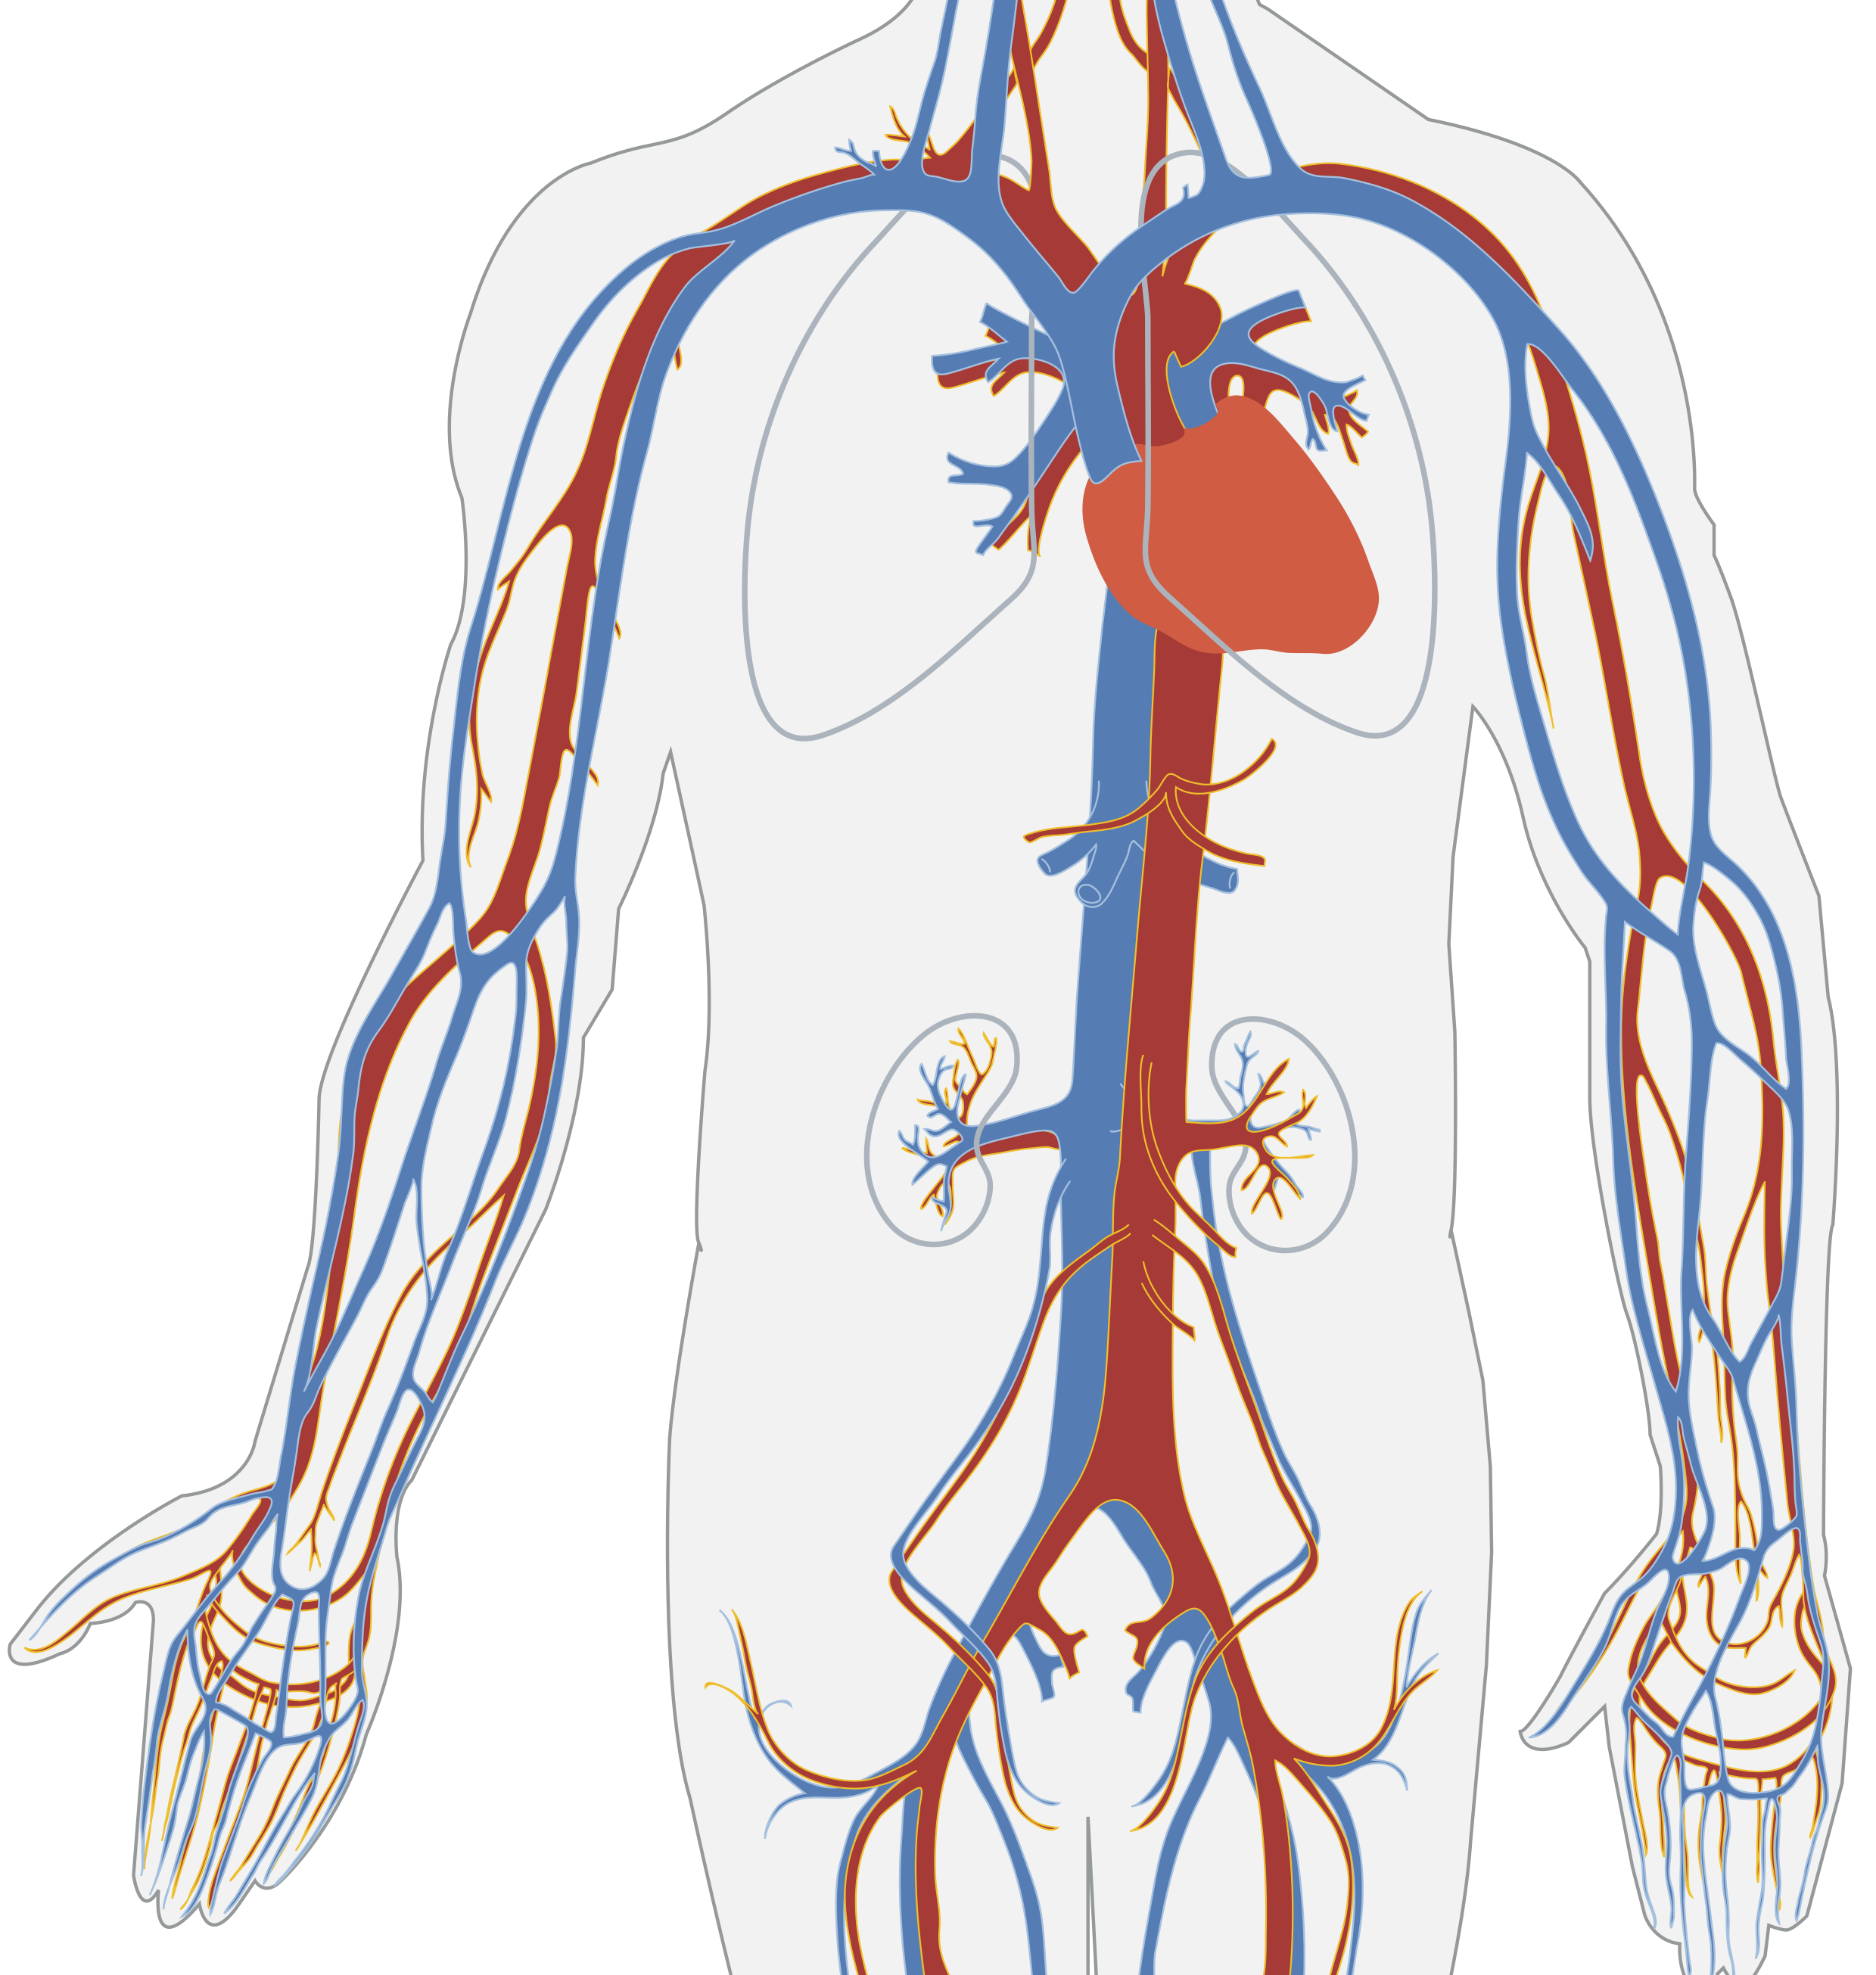
\includegraphics{ch1/Circulatory_System_no_tags_cropped.png}
\caption{Human blood circulates throughout the body and returns to the heart, veins shown in blue and arteries in red. \emph{Circulatory System en} by LadyofHats in public domain via Wikimedia Commons.}
\end{figure}

\hypertarget{galens-theory-of-blood}{%
\subsection{Galen's theory of blood}\label{galens-theory-of-blood}}

Galen came up with a different explanation based on the notion of \emph{humors}, or fluids, that was fundamental to the Greek conception of the body. He proposed that the venous and arterial blood were different humors: venous blood, or \emph{natural spirits}, was produced by the liver, while arterial blood, or \emph{vital spirits}, was produced by the heart and carried by the arteries, as shown in figure \ref{fig:galen_blood}. The heart consisted of two halves, and it warmed the blood and pushed both the natural and vital spirits out to the organs; the two spirits could mix through pores in the septum separating its right and left halves. The vital and natural spirits were both consumed by the organs, and regenerated by the liver and the heart. The purpose of the lungs was to serve as bellows, cooling the blood after it was heated by the heart.

\begin{figure}
\centering
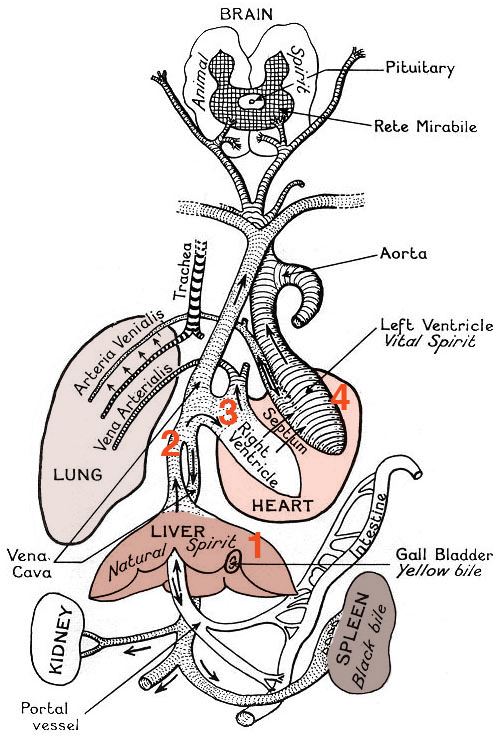
\includegraphics{ch1/galenheartc.png}
\caption{Illustration of Galen's conception of the blood system, showing different spirits traveling in one direction, but not circulating. Reproduced by permission of \href{https://faculty.humanities.uci.edu/bjbecker/}{Barbara Becker}.}
\end{figure}

Is this a good theory of how the heart, lungs, and blood work? Doctors in Europe thought so for over one thousand years! Galen's textbook on physiology was the standard for medical students through the 17th century. The theory seemed to make sense, and explain what was observable. Many great scientists and physicians, including Leonardo DaVinci and Avicenna, did not challenge the inaccuracies such as the porous septum in the heart, even though they could not see the pores themselves. It took both better observations and a quantitative testing of the hypothesis to challenge the orthodoxy.

\hypertarget{mathematical-testing-of-the-theory}{%
\subsection{Mathematical testing of the theory}\label{mathematical-testing-of-the-theory}}

William Harvey \index{Harvey, William} was born in England and studied medicine in Padua under the great physician Hieronymus Fabricius. He became famous, and would perform public demonstrations of physiology, using live animals for experiments that would not be approved today. He also studied the heart and the blood vessels, and measured the volume of the blood that can be contained in the human heart. He was quite accurate in estimating the correct volume, which we now know to be about 70 ml (1.5 oz). What is even more impressive is that he used this quantitative information to test Galen's theory.

Let us assume that all of the blood that is pumped out by the heart is consumed by the tissues, as Galen proposed; let us further assume that the heart beats at constant rate of 60 beats per minute, with a constant ejection volume of 70 ml. Then over the course of a day, the human body would consume about
\[\mathrm{Volume} = 70 \ \mathrm {mL} \times 60 \ \mathrm {(beats \ per \ minute)} \times 60 \ \mathrm {(minutes \ per \ hour)}  \times 24 \ \mathrm {(hours \ per \ day)}\]
or over 6,000 liters of blood! You may quibble over the exact numbers (some hearts beat faster or slower, some hearts may be larger or smaller) but the impact of the calculation remains the same: it is an absurd conclusion. Galen's theory would require the human being to consume and produce a quantity of fluid many times the volume of the human body (about 100 liters) in a day! This is a physical impossibility, so the only possible conclusion in that Galen's model is wrong.

This led Harvey to propose the \index{model!blood circulation}model that we know today: that blood is not consumed by the tissues, but instead returns to the heart and is re-used again \citep{schultz_william_2002}. This is why we call the heart and blood vessels part of the circulatory system of the body. This model was controversial at the time - some people proclaimed they would ``rather be wrong with Galen, than right with Harvey'\,' - but eventually became accepted as the standard model. What is remarkable is that Harvey's argument, despite being grounded in empirical data, was strictly mathematical. He adopted the assumptions of Galen, made the calculations, and got a result which was inconsistent with reality. This is an excellent example of how mathematical modeling can be useful, because it can provide clear evidence against a wrong hypothesis.

\hypertarget{sec:math1}{%
\section{Parameters and variables in models}\label{sec:math1}}

Many biologists remain skeptical of mathematical modeling. The criticism can be summarized like this: a theoretical model either agrees with experiment, or it does not. In the former case, it is useless, because the data are already known; in the latter case, it is wrong! As I indicated above, the goal of mathematical modeling is not to reproduce experimental data; otherwise, indeed, it would only be of interest to theoreticians. The correct question to ask is, does a theoretical model help us understand the real thing? There are at least three ways in which a model can be useful:

\begin{itemize}
\item
  A model can help a scientist make sense of complex data, by testing whether a particular mechanism explains the observations. Thus, a model can help clarify our understanding by throwing away the non-essential features and focusing on the most important ones.
\item
  A mathematical model makes predictions for situations that have not been observed. It is easy to change parameters in a mathematical model and calculate the effects. This can lead to new hypotheses that can be tested by experiments.
\item
  Model predictions can lead to better experimental design. Instead of trying a whole bunch of conditions, the theoretical model can suggest which ones will produce big effects, and thus can save a lot of work for the lab scientist.
\end{itemize}

In order to make a useful model of a complex living system, you have to simplify it. Even if you are only interested in a part of it, for instance a cell or a single molecule, you have to make simplifying choices. A small protein has thousands of atoms, a cell consists of millions of molecules, which all interact with each other; keeping track mathematically of every single component is daunting if not impossible. To build a useful mathematical model one must choose a few quantities which describe the system sufficiently to answer the questions of interest. For instance, if the positions of a couple of atoms in the protein you are studying determine its activity, those positions would make natural quantities to include in your model. You will find more specific examples of models later in this chapter.

Once you have decided on the essential quantities to be included in the model, these are divided into \index{variable!definition} \emph{variables} and \index{parameter} \emph{parameters}. As suggested by the name, a variable typically varies over time and the model tracks the changes in its value, while parameters usually stay constant, or change more slowly. However, that is not always the case. The most important difference is that variables describe quantities \textbf{within the system} being modeled, while parameters usually refer to quantities which are controlled by something \textbf{outside the system}.

As you can see from this definition, the same quantity can be a variable or a parameter depending on the scope of the model. Let's go back to our example of modeling a protein: usually the activity (and the structure) of a protein is influenced by external conditions such as pH and temperature; these would be natural parameters for a model of the molecule. However, if we model an entire organism, the pH (e.g.~of the blood plasma) and temperature are controlled by physiological processes within the organism, and thus these quantities will now be considered variables.

Perhaps the clearest way to differentiate between variables and parameters is to think about how you would present a data set visually. We will discuss plotting graphs of functions in chapter 2, and plotting data sets in chapter 3, but the reader has likely seen many such plots before. Consider which of the quantities you would to plot to describe the system you are modeling. If the quantity belongs on either axis, it is a variable, since it is important to describe how it changes. The rest of the quantities can be called parameters. Of course, depending on the question you ask, the same quantity may be plotted on an axis or not, which is why this classification is not absolute.

After we have specified the essential variables for your model, we can describe a complex and evolving biological system in terms of its \emph{state}. This is a very general term, but it usually means the values of all the variables that you have chosen for the model, which are often called \index{state!variable} \emph{state variables}. For instance, an ion channel can be described with the state variable of conformation, which may be in a open state or in a closed state. The range, or collection of all different states of the system is called the \index{state!space} \emph{state space} of the model. Below you will find examples of models of biological systems with diverse state spaces.

\hypertarget{discrete-state-variables-genetics}{%
\subsection{discrete state variables: genetics}\label{discrete-state-variables-genetics}}

There are genes which are present in a population as two different versions, called \index{allele}*alleles\} - let us use letters \(A\) and \(B\) to label them. One may describe the genetic state of an individual based on which allele it carries. If this individual is haploid, e.g.~a bacterium, then it only carries a single copy of the genome, and its state can be described by a single variable with the state space of \(A\) or \(B\).

A diploid organism, like a human, possesses two copies of each gene (unless it is on one of the sex chromosomes, X or Y); each copy may be in either state \(A\) or \(B\). This may seem to suggest that there are four different values in the genetic state space, but if the order of the copies does not matter (which is usually the case), then \(AB\) and \(BA\) are effectively the same, so the state space consists of three values: \(AA\), \(BB\), and \(AB\).

\hypertarget{discrete-state-variables-population}{%
\subsection{discrete state variables: population}\label{discrete-state-variables-population}}

Consider the model of a population of individuals, with the variable of number of individuals (populations size) and parameters being the birth and death rates. The state space of this model is \textbf{all integers between 0 and infinity.}

Consider the model of a population of individuals who may get infected. Assume that the total number of individuals does not change (that is, there are no births and deaths) and that these individuals can be in one of two states: healthy or sick (in epidemiology these are called \emph{susceptible} or \emph{infectious}). There are typically two parameters in such models: the probability of infection and the probability of recovery. Since the total population is fixed at some number \(N\), the space space of the model is all pairs of integers between 0 and \(N\) that add up to \(N\).

\hypertarget{continuous-state-variables-concentration}{%
\subsection{continuous state variables: concentration}\label{continuous-state-variables-concentration}}

Suppose that a biological molecule is produced with a certain rate and degraded with a different rate, and we would like to describe the quantity of the molecule, usually expressed as concentration. The relevant variables here are concentration and time, and you will see those variables on the axes of many plots in biochemistry. Concentration is a ratio of the number of molecules and the volume, so the state space can be any positive real number (although practically there is a limit as to how many molecules can fit inside a given volume, but for simplicity we can ignore this).

Going even further, let us consider an entire cell, which contains a large number of different molecules. We can describe the state of a cell as the collection of all the molecular concentrations, with the parameters being the rates of all the reactions going on between those molecules. The state space for this model with \(N\) different molecules is \(N\) positive real numbers.

\hypertarget{multiple-variables-in-medicine}{%
\subsection{multiple variables in medicine}\label{multiple-variables-in-medicine}}

Doctors take medical history from patients and measure vital signs to get a picture of a patient's health. These can be all be thought of as variables in a model of a person that physicians construct. Some of these variables are discrete, for instance whether there is family history of hypertension, which has only two values: yes or no. Other variables are numbers with a range, such as weight and blood pressure. The state space of this model is a combination of \emph{categorical} values (such as yes/no) and \emph{numerical} values (within a reasonable range).

\hypertarget{discussion-questions}{%
\subsection{Discussion questions}\label{discussion-questions}}

Several biological models are indicated below. Based on what you know, divide the quantities into variables and parameters and describe the state space of the model. Note that there may be more than one correct interpretation

\begin{enumerate}
\def\labelenumi{\arabic{enumi}.}
\item
  The volume of blood pumped by the heart over a certain amount of time, depending on the heart rate and the ejection volume.
\item
  The number of wolves in a national forest depending on the number of wolves in the previous year, the birth rate, the death rate, and the migration rate.
\item
  The fraction of hemes in hemoglobin (a transport protein in red blood cells) which are bound to oxygen depending on the partial pressure of oxygen and the binding cooperativity of hemoglobin.
\item
  The number of mutations that occur in a genome, depending on the mutation rate, the amount of time, and the length of the genome.
\item
  The concentration of a drug in the blood stream depending on the dose, time after administration, and the rate of metabolism (processing) of the drug.
\item
  Describing an outbreak of an infectious disease in a city in terms of the fractions of infected, healthy, and recovered people, depending on the rate of infection, rate of recovery, and the mortality rate of the disease.
\end{enumerate}

\hypertarget{first-steps-in-r}{%
\section{First steps in R}\label{first-steps-in-r}}

\label{sec:comp1}
A central goal of this book is to help you, the reader, gain experience with computation, which requires learning some programming (cool kids call it ``coding''). Programming is a way of interacting with computers through a symbolic language, unlike the graphic user interfaces that we're all familiar with. Basically, programming allows you to make a computer do exactly what you want it to do.

There is a vast number of computer languages with distinct functionalities and personalities. Some are made to talk directly to the computer's ``brain'' (CPU and memory), e.g.~Assembly, while others are better suited for human comprehension, e.g.~python or Java. Programming in any language involves two parts: 1) writing a program (code) using the commands and the syntax for the language; 2) running the code by using a compiler or interpreter to translate the commands into machine language and then making the computer execute the actions. If your code has a mistake in it, the compiler or interpreter should catch it, and return an \emph{error message} to you instead of executing the code. Sometimes, though, the code may pass muster with the interpreter/compiler, but it may still have a mistake (bug). This can be manifested in two different ways: either the code execution does not produce the result that you intended, or it hangs up or crashes the computer (the latter is hard to do with the kind of programming we will be doing). We will discuss errors and how to prevent and catch these bugs as you develop your programming skills.

In this course, our goal is to compute mathematical models and to analyze data, so we choose a language that is designed specially for these tasks, which is called R. To proceed, you'll need to download and install R, which is freely available \href{cran.r-project.org/}{here}. In addition to downloading the language (which includes the interpreter that allows you to run R code on your computer) you will need to download a graphic interface for writing, editing, and running R code, called R Studio (coders call this an IDE, or an Integrated Developer Environment), which is also free and available \href{www.rstudio.com/products/rstudio/download/}{here}.

\hypertarget{r-markdown-and-r-studio}{%
\subsection{R Markdown and R Studio}\label{r-markdown-and-r-studio}}

In this course you will use R using R Studio and R Markdown documents, which are text files with the extension \texttt{.Rmd}. Markdown is a simple formatting syntax for creating reports in HTML, PDF, or Word format by incorporating text with code and its output. More details on using R Markdown are \href{rmarkdown.rstudio.com}{here}. In fact, this whole book is written in R Markdown files and then compiled to produce the beautiful (I hope you agree) web book that you are reading.

If you open an Rmd file in R Studio, you will see a \textbf{Knit} button on top of the Editor window. Clicking it initiates the processing of the file into an output document (in HTML, PDF, or Word format) that includes the text as well as the output of any embedded R code chunks within the document. You can embed an R \emph{code chunk} like this:

\begin{Shaded}
\begin{Highlighting}[]
\KeywordTok{print}\NormalTok{(}\StringTok{"Hello there!"}\NormalTok{) }
\end{Highlighting}
\end{Shaded}

\begin{verbatim}
## [1] "Hello there!"
\end{verbatim}

To run the code inside a single R code chunk, click the green arrow in the top right of the chunk. This will produce an output, in this case the text ``Hello there!''. Inside the generated output file, for example the web book you may be reading, the output of code chunks is shown below the box with the R code and indicated by two hashtags.

You can make text \textbf{bold} or \emph{italic} like so. You can also use mathematical notation called LaTeX, which you'll see used below to generate nice-looking equations. LaTeX commands are surrounded by dollar signs, for example \$e\^{}x\$ generates \(e^x\). Mathematical types love LaTeX, but you can use R Markdown without it.

\hypertarget{numbers-and-arithmetic-operations}{%
\subsection{numbers and arithmetic operations}\label{numbers-and-arithmetic-operations}}

When you get down to the brass tacks, all computation rests on performing \index{R programming!arithmetic} \emph{arithmetic operations}: addition, subtraction, multiplication, division, exponentiation, etc. The symbols used for arithmetic operations are what you'd expect: \texttt{+}, \texttt{-}, \texttt{*}, \texttt{/} are the four standard operations, and \texttt{\^{}} is the symbol for exponentiation. For example, type \texttt{2\^{}3} in any R code chunk and execute it:

\begin{Shaded}
\begin{Highlighting}[]
\DecValTok{2}\OperatorTok{\^{}}\DecValTok{3}
\end{Highlighting}
\end{Shaded}

\begin{verbatim}
## [1] 8
\end{verbatim}

You see that R returns the result by printing it out on the screen. The number in square brackets {[}1{]} is not important for now; it is useful when the answer contains many numbers and has to be printed out on many rows. The second number is the result of the calculation.

For numbers that are either very large or very small, it's too cumbersome to write out all the digits, so R, like most computational platforms, uses the \index{R programming!scientific notation}\emph{scientific notation}. For instance, if you want to represent 1.4 billion, you type in the following command; note that 10 to the ninth power is represented as \texttt{e+09} and the prefix 1.4 is written without any multiplication sign:

\begin{Shaded}
\begin{Highlighting}[]
\FloatTok{1.4}\OperatorTok{*}\DecValTok{10}\OperatorTok{\^{}}\DecValTok{9}
\end{Highlighting}
\end{Shaded}

\begin{verbatim}
## [1] 1.4e+09
\end{verbatim}

There are also certain numbers built into the R language, most notably \(\pi\) and \(e\), which can be accessed as follows:

\begin{Shaded}
\begin{Highlighting}[]
\NormalTok{pi}
\end{Highlighting}
\end{Shaded}

\begin{verbatim}
## [1] 3.141593
\end{verbatim}

\begin{Shaded}
\begin{Highlighting}[]
\KeywordTok{exp}\NormalTok{(}\DecValTok{1}\NormalTok{)}
\end{Highlighting}
\end{Shaded}

\begin{verbatim}
## [1] 2.718282
\end{verbatim}

The expression \texttt{exp()} is an example of a function, which we will discuss in section \ref{sec:comp2}; it returns the value of \(e\) raised to the power of the number in parenthesis, hence \texttt{exp(1)} returns \(e\). Notice that although both numbers are irrational, and thus have infinitely many decimal digits, R only prints out a few of them. This doesn't mean that it doesn't have more digits in memory, but it only displays a limited number to avoid clutter. The number of digits to be displayed can be changed, for example to display 10 digits, type in \texttt{options(digits=10)}.

Computers are very good at computation, as their name suggests, but they have limitations. In order to manipulate numbers, they must be stored in computer memory, but computer memory is finite. There is a limit to the length of the number that is feasible to store on a computer. This has implications for both very large numbers and to very small numbers, which are close to zero, because both require many digits for storage.

All programming languages have an upper limit on the biggest number it will store and work with. If an arithmetic operation results in a number larger than that limit, the computer will call it an \emph{overflow} error. Depending on the language, this may stop the execution of the program, or else produce a non-numerical value, such as \texttt{NaN} (not a number) or \texttt{Inf} (infinite). Do exercise \ref{ex:overflow} to investigate the limitations of R for large numbers.

On the other hand, very small numbers present their own challenges. As with very large numbers, a computer cannot store an arbitrary number of digits after the decimal (or binary) point. Therefore, there is also the smallest number that a programming language will accept and use, and storing a smaller number produces an \emph{underflow} error. This will either cause the program execution to stop, or to return the value 0 instead of the correct answer. Do exercise \ref{ex:underflow} to investigate the limitations of R for small numbers.

This last fact demonstrates that all computer operations are imprecise, as they are limited by what's called the \index{R programming!machine precision} \emph{machine precision}, which is illustrated in exercise \ref{ex:mach_prec}. For instance, two similar numbers, if they are within the machine precision of one another, will be considered the same by the computer. Modern computers have large memories, and their machine precision is very good, but sometimes this error presents a problem, e.g.~when subtracting two numbers. A detailed discussion of machine error is beyond the scope of this text, but anyone performing computations must be aware of its inherent limitations.

\hypertarget{r-coding-exercises}{%
\subsection{R Coding Exercises}\label{r-coding-exercises}}

\begin{enumerate}
\def\labelenumi{\arabic{enumi}.}
\item
  Calculate the value of \(\pi\) raised to the 10th power.
\item
  Use the scientific notation to multiply four billion by \(\pi\).
\item
  Use the scientific notation with large exponents (e.g.~1e+100, 1e+500, etc.) to find out what happens when you give R a number that is too large for it to handle. Approximately at what order of magnitude does R produce an overflow error?
\item
  In the same fashion, find out what happens when you give R a number that is too small for it to handle. Approximately at what order of magnitude does R produce an underflow error?
\item
  How close can two numbers be before R thinks they are the same? Subtract two numbers which are close to each other, like 24 and 24.001, and keep making them closer to each other, until R returns a difference of zero. Report at what value of the actual difference this happens.
\end{enumerate}

\hypertarget{variable-assignment}{%
\subsection{variable assignment}\label{variable-assignment}}

Variables in programming languages are used to store and access numerical or other information. After \index{variable!assignment}\emph{assigning}\} it a value for the first time (\emph{initializing}), a variable name can be used to represent the value we assigned to it. Invoking the name of variable recalls the stored value from computer's memory. There are a few rules about naming variables: a name cannot be a number or an arithmetic operator like \texttt{+}, in fact it cannot contain symbols for operators or spaces inside the name, or else confusion would reign. Variable names may contain numbers, but not as the first character. When writing code it is good practice to give variables informative names, like \emph{height} or \emph{city\_pop}. \index{R programming!variable assignment}

The symbol `=' is used to assign a value to a variable in most programming languages, and can be used in R too. However, it is customary for R to use the symbols \texttt{\textless{}-} together to indicate assignment, like this:

\begin{Shaded}
\begin{Highlighting}[]
\NormalTok{var1 \textless{}{-}}\StringTok{ }\DecValTok{5}
\end{Highlighting}
\end{Shaded}

After this command the variable \texttt{var1} has the value 5, which you can see in the upper right frame in R Studio called \emph{Environment}. In order to display the value of the variable as an output on the screen, use the special command \texttt{print()} (it's actually a function, which we will discuss in the next chapter). The following two commands show that the value of a variable can be changed after it has been initialized:

\begin{Shaded}
\begin{Highlighting}[]
\NormalTok{var1 \textless{}{-}}\StringTok{ }\DecValTok{5}
\NormalTok{var1 \textless{}{-}}\StringTok{ }\DecValTok{6}
\KeywordTok{print}\NormalTok{(var1)}
\end{Highlighting}
\end{Shaded}

\begin{verbatim}
## [1] 6
\end{verbatim}

While seemingly contradictory, the commands are perfectly clear to the computer: first \texttt{var1} is assigned the value 5 and then it is assigned 6. After the second command, the first value is forgotten, so any operations that use the variable \texttt{var1} will be using the value of 6.

Entire expressions can be placed on the right hand side of an assignment command: they could be arithmetic or logical operations as well as functions, which we will discuss later on. For example, the following commands result in the value 6 being assigned to the variable \texttt{var2}:

\begin{Shaded}
\begin{Highlighting}[]
\NormalTok{var1 \textless{}{-}}\StringTok{ }\DecValTok{5}
\NormalTok{var2 \textless{}{-}}\StringTok{ }\NormalTok{var1}\OperatorTok{+}\DecValTok{1}
\KeywordTok{print}\NormalTok{(var2)}
\end{Highlighting}
\end{Shaded}

\begin{verbatim}
## [1] 6
\end{verbatim}

Even more mind-blowing is that the same variable can be used on both sides of an assignment operator! The R interpreter first looks on the right hand side to evaluate the expression and then assigns the result to the variable name on the left hand side. So for instance, the following commands increase the value of \texttt{var1} by 1, and then assign the product of \texttt{var1} and \texttt{var2} to the variable \texttt{var2}:

\begin{Shaded}
\begin{Highlighting}[]
\NormalTok{var1 \textless{}{-}}\StringTok{ }\NormalTok{var1 }\OperatorTok{+}\StringTok{ }\DecValTok{1}
\KeywordTok{print}\NormalTok{(var1)}
\end{Highlighting}
\end{Shaded}

\begin{verbatim}
## [1] 6
\end{verbatim}

\begin{Shaded}
\begin{Highlighting}[]
\NormalTok{var2 \textless{}{-}}\StringTok{ }\NormalTok{var1}\DecValTok{{-}1}
\KeywordTok{print}\NormalTok{(var2)}
\end{Highlighting}
\end{Shaded}

\begin{verbatim}
## [1] 5
\end{verbatim}

\begin{Shaded}
\begin{Highlighting}[]
\NormalTok{var2 \textless{}{-}}\StringTok{ }\NormalTok{var1}\OperatorTok{*}\NormalTok{var2}
\KeywordTok{print}\NormalTok{(var2)}
\end{Highlighting}
\end{Shaded}

\begin{verbatim}
## [1] 30
\end{verbatim}

We have seen example of how to assign values to variables, so here is an example of how NOT to assign values, with the resulting error message:

\begin{Shaded}
\begin{Highlighting}[]
\NormalTok{var1 }\OperatorTok{+}\StringTok{ }\DecValTok{1}\NormalTok{ \textless{}{-}}\StringTok{ }\NormalTok{var1}
\end{Highlighting}
\end{Shaded}

The left-hand side of an assignment command should contain only the variable to which you are assigning a value, not an arithmetic expression to be performed.

\hypertarget{r-coding-exercises-1}{%
\subsection{R Coding Exercises}\label{r-coding-exercises-1}}

The following commands or scripts do not work as intended. Find the errors and correct them, then run them to make sure they do what they are intended to do:

\hypertarget{exercises}{%
\subsection{Exercises:}\label{exercises}}

The following R commands or short scripts contain errors; your job is to fix them so they runs as described. (Remove the \# at the start of each line to ``uncomment'' the code first.)

\begin{enumerate}
\def\labelenumi{\arabic{enumi}.}
\tightlist
\item
  Assign the value -10 to a variable
\end{enumerate}

\begin{Shaded}
\begin{Highlighting}[]
\NormalTok{neg {-}\textgreater{}}\StringTok{ }\DecValTok{{-}10}
\end{Highlighting}
\end{Shaded}

\begin{enumerate}
\def\labelenumi{\arabic{enumi}.}
\setcounter{enumi}{1}
\tightlist
\item
  Assign a variable the value 5 and then increase its value by 3:
\end{enumerate}

\begin{Shaded}
\begin{Highlighting}[]
\NormalTok{2pac \textless{}{-}}\StringTok{ }\DecValTok{5}
\NormalTok{2pac \textless{}{-}}\StringTok{ }\NormalTok{2pac }\OperatorTok{+}\StringTok{ }\DecValTok{3}
\end{Highlighting}
\end{Shaded}

\begin{enumerate}
\def\labelenumi{\arabic{enumi}.}
\setcounter{enumi}{2}
\tightlist
\item
  Assign the values 4 and 7 to two variables, then add them together and assign the sum to a new variable:
\end{enumerate}

\begin{Shaded}
\begin{Highlighting}[]
\NormalTok{total \textless{}{-}}\StringTok{ }\NormalTok{part1 }\OperatorTok{+}\StringTok{ }\NormalTok{part2}
\NormalTok{part1 \textless{}{-}}\StringTok{ }\DecValTok{4}
\NormalTok{part2 \textless{}{-}}\StringTok{ }\DecValTok{7}
\end{Highlighting}
\end{Shaded}

\begin{enumerate}
\def\labelenumi{\arabic{enumi}.}
\setcounter{enumi}{3}
\tightlist
\item
  Add 5 and 3 and save it into variable my.number
\end{enumerate}

\begin{Shaded}
\begin{Highlighting}[]
\DecValTok{5} \OperatorTok{+}\StringTok{ }\DecValTok{3}\NormalTok{ \textless{}{-}}\StringTok{ }\NormalTok{my.number}
\end{Highlighting}
\end{Shaded}

\begin{enumerate}
\def\labelenumi{\arabic{enumi}.}
\setcounter{enumi}{4}
\tightlist
\item
  Print the value of my.number on the screen:
\end{enumerate}

\begin{Shaded}
\begin{Highlighting}[]
\NormalTok{print[my.number]}
\end{Highlighting}
\end{Shaded}

\begin{enumerate}
\def\labelenumi{\arabic{enumi}.}
\setcounter{enumi}{5}
\tightlist
\item
  Replace the value of my.number with 5 times its current value
\end{enumerate}

\begin{Shaded}
\begin{Highlighting}[]
\NormalTok{my.number \textless{}{-}}\StringTok{ }\NormalTok{5my.number }
\end{Highlighting}
\end{Shaded}

\begin{enumerate}
\def\labelenumi{\arabic{enumi}.}
\setcounter{enumi}{6}
\tightlist
\item
  Assign the values of 7 and 8 to variables a and b, respectively, multiply them and save the results in variable x
\end{enumerate}

\begin{Shaded}
\begin{Highlighting}[]
\NormalTok{a\textless{}{-}}\DecValTok{7}
\NormalTok{b\textless{}{-}}\DecValTok{8}
\NormalTok{x\textless{}{-}ab}
\KeywordTok{print}\NormalTok{(x)}
\end{Highlighting}
\end{Shaded}

\begin{enumerate}
\def\labelenumi{\arabic{enumi}.}
\setcounter{enumi}{8}
\tightlist
\item
  Assign the value 42 to a variable, then increase it by 1
\end{enumerate}

\begin{Shaded}
\begin{Highlighting}[]
\NormalTok{age \textless{}{-}}\StringTok{ }\DecValTok{42}
\NormalTok{age }\OperatorTok{+}\StringTok{ }\DecValTok{1}\NormalTok{ \textless{}{-}}\StringTok{ }\NormalTok{age}
\end{Highlighting}
\end{Shaded}

\begin{enumerate}
\def\labelenumi{\arabic{enumi}.}
\setcounter{enumi}{9}
\tightlist
\item
  Assign the value 10 to variable radius, then calculate the area of the circle with that radius using the formula \(A = \pi r^2\):
\end{enumerate}

\begin{Shaded}
\begin{Highlighting}[]
\NormalTok{r \textless{}{-}}\StringTok{ }\DecValTok{10}
\NormalTok{area \textless{}{-}}\StringTok{ }\NormalTok{pir}\OperatorTok{\^{}}\DecValTok{2} 
\end{Highlighting}
\end{Shaded}

\hypertarget{r-assignment}{%
\section{R Assignment}\label{r-assignment}}

In the following tasks you will translate mathematical models into R commands and make the computer perform calculations. The first step is to give descriptive names to these variables (instead of single letters!), and then use these variables to calculate the predictions of the models.

\begin{enumerate}
\def\labelenumi{\arabic{enumi}.}
\tightlist
\item
  Take the model of a heart pumping with a constant rate, where V is the total volume of blood pumped by the heart over time, S is the stroke volume, \(R\) is the heart rate and \(t\) is time:
\end{enumerate}

\[ 
V = SRt
\]

For a heart beating at 60 beats per minute with stroke volume of 75 ml over 80 minutes, create variables for the stroke volume, heart rate, and time (come up with your own descriptive names). Calculate the total volume pumped by the heart by turning the equation into a line of R code, assigning the result to a variable, and print out the result. ANSWER: 360000 ml

\begin{Shaded}
\begin{Highlighting}[]
\CommentTok{\# THIS IS A COMMENT. YOUR CODE GOES HERE }
\end{Highlighting}
\end{Shaded}

\begin{enumerate}
\def\labelenumi{\arabic{enumi}.}
\setcounter{enumi}{1}
\tightlist
\item
  Consider an infectious disease that spreads through a new population at an exponential rate r (per day). If there are initially I infected individuals, then after t days the model predicts the total number of infected to be T:
\end{enumerate}

\[ 
T = I(1+r)^t
\]

If the initial number of infected is 20, and the rate of spread is 8\% per day, calculate the total number of infected after 30 days by assigning these values to informatively named variables, turning the equation above into a line of R code, assigning the result to a variable, and print out the result. ANSWER: 201.2531 infected

\begin{Shaded}
\begin{Highlighting}[]
\CommentTok{\# THIS IS A COMMENT. YOUR CODE GOES HERE }
\end{Highlighting}
\end{Shaded}

\begin{enumerate}
\def\labelenumi{\arabic{enumi}.}
\setcounter{enumi}{2}
\tightlist
\item
  The logistic model for a population P that is limited to a certain number, called carrying capacity K (population size), can be written as follows, with t time (years), r the intrinsic growth rate (per year) and A a dimensionless constant.
\end{enumerate}

\[
P= \frac{K}{1 + A e^{-rt}}
\]
Let K be 30000, r be 0.08, and A be 29, assign these values to informatively named variables. Calculate the population size after 25 years by turning the equation above into a line of R code, assigning the result to a variable, and print out the result. ANSWER: 6091.713 individuals

\begin{Shaded}
\begin{Highlighting}[]
\CommentTok{\# THIS IS A COMMENT. YOUR CODE GOES HERE }
\end{Highlighting}
\end{Shaded}

\hypertarget{functions-and-their-graphs}{%
\chapter{Functions and their graphs}\label{functions-and-their-graphs}}

\begin{quote}
Some fathers, if you ask them for the time of day, spit silver dollars.\\
Donald Barthelme, \emph{The Dead Father}
\end{quote}

Mathematical models describe how various quantities affect each other. In the last chapter we learned that these descriptions can be written down, often in the form of an equation. For instance, we can describe the total volume of blood pumped over a period of time as the product of stroke volume, the heart rate and the number of minutes, which can be written as an equation. The different quantities have their own meaning and roles, depending on what they stand for. To better describe how these quantities are related we use the deep idea of mathematical functions. In this chapter you will learn to do the following:

\begin{itemize}
\tightlist
\item
  use dimensional analysis to deduce the meaning of quantities in a model
\item
  understand the concept of function, dependent and independent variables
\item
  recognize basic functional forms and the shape of their graphs
\item
  use R to plot functions
\item
  understand basic models of reaction rates
\end{itemize}

\hypertarget{sec:model2}{%
\section{Dimensions of quantities}\label{sec:model2}}

What distinguishes a mathematical model from a mathematical equation is that the quantities involved have a real-world meaning. Each quantity represents a measurement, and associated with each one are the \index{units} \emph{units} of measurement. The number 173 is not enough to describe the height of a person - you are left to wonder 173 what? meters, centimeters, nanometers, light-years? Obviously, only centimeters make sense as a unit of measurement for human height; but if we were measuring the distance between two animals in a habitat, meters would be a reasonable unit, and it were the distance between molecules in a cell, we would use nanometers. Thus, any quantity in a mathematical model must have associated units, and any graphs of these quantities must be labeled accordingly.

In addition to units, each variable and parameter has a meaning, which is called the \index{dimension} \emph{dimension} of the quantity. For example, any measurement of length or distance has the same dimension, although the units may vary. The value of a quantity depends on the units of measurement, but its essential dimensionality does not. One can convert a measurement in meters to that in light-years or cubits, but one cannot convert a measurement in number of sheep to seconds - that conversion has no meaning.

Thus leads us to the fundamental rule of mathematical modeling: \textbf{terms that are added or subtracted must have the same dimension}. This gives mathematical modelers a useful tool called \index{dimensional analysis} \emph{dimensional analysis}, which involves replacing the quantities in an equation with their dimensions. This serves as a check that all dimensions match, as well as allowing to deduce the dimensions of any parameters for which the dimension was not specified. \citep{smith_mathematical_1968}

\textbf{Example.} As we saw in chapter 1, the relationship between the amount blood pumped by a heart in a certain amount of time is expressed in the following equation, where \(V_{tot}\) and \(V_s\) are the total volume and stroke volume, respectively, \(R\) is the heart rate, and \(t\) is the time:
\[
V_{tot} = V_sRt
\]
The dimension of a quantity \(X\) is denoted by \([X]\); for example, if \(t\) has the dimension of time, we write \([t] = time\). The dimension of volume is \([V_{tot}] = length^3\), the dimension of stroke volume is \([V_s] = volume/beat\) and the dimension of time \(t\) is time, so we can re-write the equation above in dimensional form:

\[length^3 = length^3/ beat \times R \times time\]

Solving this equation for R, we find that it must have the dimensions of \([R] = beats/time\). It can be measured in beats per minute (typical for heart rate), or beats per second, beats per hour, etc. but the
\emph{dimensionality} of the quantity cannot be changed without making the model meaningless.

There are also \index{dimensionless quantity} \emph{dimensionless} quantities, or pure numbers, which are not tied to a physical meaning at all. Fundamental mathematical constants, like \(\pi\) or \(e\), are classic examples, as are some important quantities in physics, like the Reynolds number in fluid mechanics. \citep{strogatz_nonlinear_2001} Quantities with a dimension can be made dimensionless by dividing them by another quantity with the same dimension and ``canceling'' the dimensions. For instance, we can express the height of a person as a fraction of the mean height of the population; then the height of a tall person will become a number greater than 1, and the height of a short one will become less than 1. This new dimensionless height does not have units of length - they have been divided out by the mean height. This is known as \index{rescaling} \emph{rescaling} the quantity, by dividing it by a preferred scale. There is a fundamental difference between rescaling and changing the units of a quantity: when changing the units, e.g.~from inches to centimeters, the dimension remains the same, but if one divides the quantity by a scale, it loses its dimension.

\textbf{Example.} The model for a population of bacteria that doubles every hour is described by the equation, where \(P_0\) is initial number of bacteria and \(P\) is the population after \(t\) hours:
\[ P = P_0 2^t \]
Let us define the quantity \(R=P/P_0\), so we can say that population increased by a factor of \(R\) after \(t\) hours. This ratio is a dimensionless quantity because \(P\) and \(P_0\) have the same dimension of bacterial population, which cancel out. The equation for \(R\) can be written as follows:
\[ R= 2^t \]
According to dimensional analysis, both sides of the equation have to be dimensionless, so \(t\) must also be a dimensionless variable. This is surprising, because \(t\) indicates the number of hours the bacterial colony has been growing. This reveals the subtle fact that \(t\) is a rescaled variable obtained by dividing the elapsed time by the length of the reproductive cycle. Because of the assumption that the bacteria divide exactly once an hour, \(t\) counts the number of hours, but if they divided once a day, \(t\) would denote the number of days. So \(t\) doesn't have units or dimensions, but instead denotes the dimensionless number of cell divisions.

\hypertarget{exercises-1}{%
\subsection{Exercises}\label{exercises-1}}

For each biological model below determine the dimensions of the parameters, based on the given dimensions of the variables.

\begin{enumerate}
\def\labelenumi{\arabic{enumi}.}
\item
  Model of number of mutations \(M\) as a function of time \(t\):
  \[ M(t) = M_0 + \mu t\]
\item
  Model of molecular concentration \(C\) as a function of time \(t\):
  \[ C(t) = C_0 e^{-kt} \]
\item
  Model of tree height \(H\) (length) as a function of age \(a\) (time):
  \[ H(a) = \frac{b a}{c + a}\]
\item
  Model of cooperative binding of ligands, with fraction of bound receptors \(\theta\) as a function of ligand concentration \(L\):
  \[ \theta (L) = \frac{L^n}{L^n + K_d}\]
\item
  Model of concentration of a gene product \(G\) (concentration) as a function of time \(t\):
  \[ G(t) = G_m (1 - e^{-\alpha t})\]
\item
  Michaelis-Menten model of enzyme kinetics, \(v\) is reaction rate (1/time) and \(S\) is substrate concentration:
  \[ v(S) = \frac{v_{max} S}{K_m + S}\]
\item
  Logistic model of population growth, \(P\) is population size and time \(t\):
  \[ P(t) = \frac{A e^{kt}}{1 + B(e^{kt} -1)} \]
\end{enumerate}

\hypertarget{sec:math2}{%
\section{Functions and their graphs}\label{sec:math2}}

A relationship between two variables addresses the basic question: when one variable changes, how does this affect the other? An equation, like the examples in the last section, allows one to calculate the value of one variable based on the other variable and parameter values. In this section we seek to describe more broadly how two variables are related by using the mathematical concept of functions.

\begin{definition}
\protect\hypertarget{def:def-function}{}{\label{def:def-function} }A function is a mathematical rule which has an input and an output. A function returns a well-defined output for every input, that is, for a given input value the function returns a unique output value.
\end{definition}

In this abstract definition of a function it doesn't have to be written as an algebraic equation, it only has to return a unique output for any given input value. In mathematics we usually write them down in terms of algebraic expressions. As in mathematical models, you will see two different kinds of quantities in equations that define functions: variables and parameters. The input and the output of a function are usually variables, with the input called the \index{variable!independent} \emph{independent variable} and the output called the \index{variable!dependent} \emph{dependent variable}.

The relationship between the input and the output can be graphically illustrated in a \index{function!graph} graph, which is a collection of paired values of the independent and dependent variable drawn as a curve in the plane. Although it shows how the two variables change relative to each other, parameters may change too, which results in a different graph of the function. While graphing calculators and computers can draw graphs for you, it is very helpful to have an intuitive understanding about how a function behaves, and how the behavior depends on the parameters. Here are the three questions to help picture the relationship (assume \(x\) is the independent variable and it is a nonnegative real number):

\begin{enumerate}
\def\labelenumi{\arabic{enumi}.}
\tightlist
\item
  what is the value of the function at \(x=0\)?
\item
  what does the function do when \(x\) becomes large (\(x \to \infty\))?
\item
  what does the function do between the two extremes?
\end{enumerate}

Below you will find examples of fundamental functions used in biological models with descriptions of how their parameters influence their graphs.

\hypertarget{linear-and-exponential-functions}{%
\subsection{linear and exponential functions}\label{linear-and-exponential-functions}}

The reader is probably familiar with linear and exponential functions from algebra courses. However, they are so commonly used that it is worth going over them to refresh your memory and perhaps to see them from another perspective.

\begin{definition}
\protect\hypertarget{def:def-linfunc}{}{\label{def:def-linfunc} }A \emph{linear function} \(f(x)\) is one for which the difference in two function values is the same for a specific difference in the independent variable.
\end{definition}

In mathematical terms, this can be written an equation for any two values of the independent variable \(x_1\) and \(x_2\) and a difference \(\Delta x\):

\[ f(x_1 + \Delta x) - f(x_1) = f(x_2 + \Delta x) - f(x_2) \]
The general form of the linear function is written as follows:
\begin{equation}
f(x) = ax + b
\label{eq:linear_funk}
\end{equation}

The function contains two parameters: the \index{slope!linear function}\index{linear!slope} slope \(a\) and the \index{y-intercept!linear function} y-intercept \(b\). The graph of the linear function is a line (hence the name) and the slope \(a\) determines its steepness. A positive slope corresponds to the graph that increases as \(x\) increases, and a negative slope corresponds to a declining function. At \(x=0\), the function equals \(b\), and as \(x \to \infty\), the function approaches positive infinity if \(a>0\), and approaches negative infinity if \(a<0\).

\begin{definition}
\protect\hypertarget{def:def-expfun}{}{\label{def:def-expfun} }An \emph{exponential function} \(f(x)\) is one for which the ratio of two function values is the same for a specific difference in the independent variable.
\end{definition}

Mathematically speaking, this can be written as follows for any two values of the independent variable \(x_1\) and \(x_2\) and a difference \(\Delta x\):
\[ \frac{f(x_1 + \Delta x)}{f(x_1)} = \frac{f(x_2 + \Delta x)}{f(x_2)}\]

Exponential functions can be written using different symbolic forms, but they all have a constant base with the variable \(x\) in the exponent. I prefer to use the constant \(e\) (base of the natural logarithm) as the base of all the exponential functions, for reasons that will become apparent in chapter 15. This does not restrict the range of possible functions, because any exponential function can be expressed using base \(e\), using a transformation: \(a^x = e^{x \ln(a)}\). So let us agree to write exponential functions in the following form:
\begin{equation}
 f(x) = a e^{rx}
\label{eq:exp_funk}
\end{equation}

The function contains two parameters: the \index{exponential!rate constant}\emph{rate constant} \(r\) and the multiplicative constant \(a\). The graph of the exponential function is a curve which crosses the y-axis at \(y=a\) (plug in \(x=0\) to see that this is the case). As \(x\) increases, the behavior of the graph depends on the sign of the rate constant \(r\). If \(r>0\), the function approaches infinity (positive if \(a>0\), negative if \(a<0\)) as \(x \to \infty\). If \(r<0\), the function decays at an ever-decreasing pace and asymptotically approaches zero as \(x \to \infty\). Thus the graph of \(f(x)\) is a curve either going to infinity or a curve asymptotically approaching 0, and the steepness of the growth or decay is determined by \(r\).

\begin{figure}

{\centering 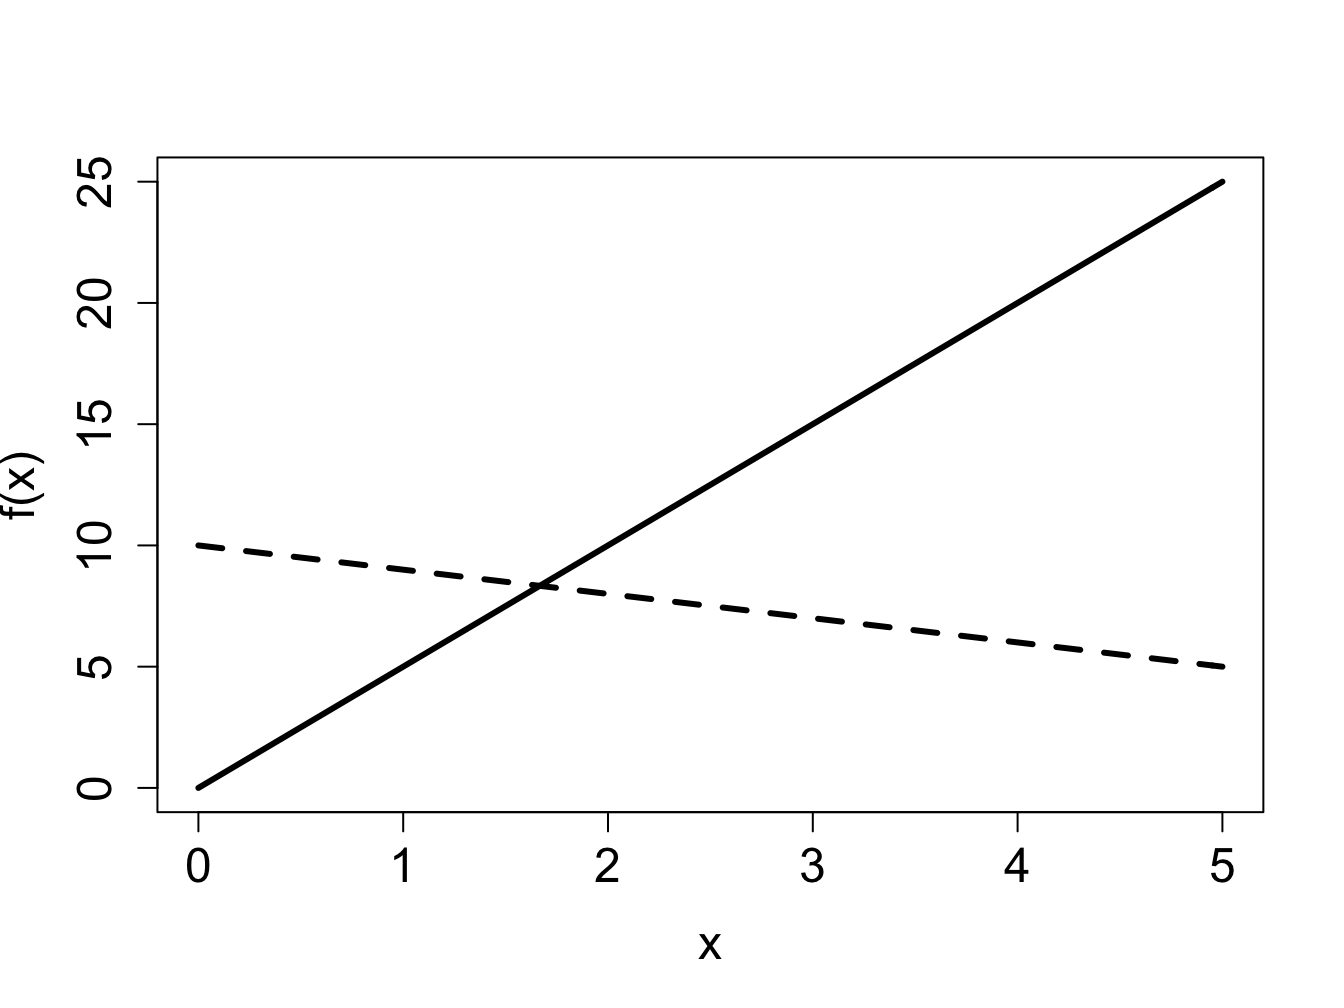
\includegraphics[width=0.5\linewidth]{QuantLife_files/figure-latex/ch2-funk1-1} 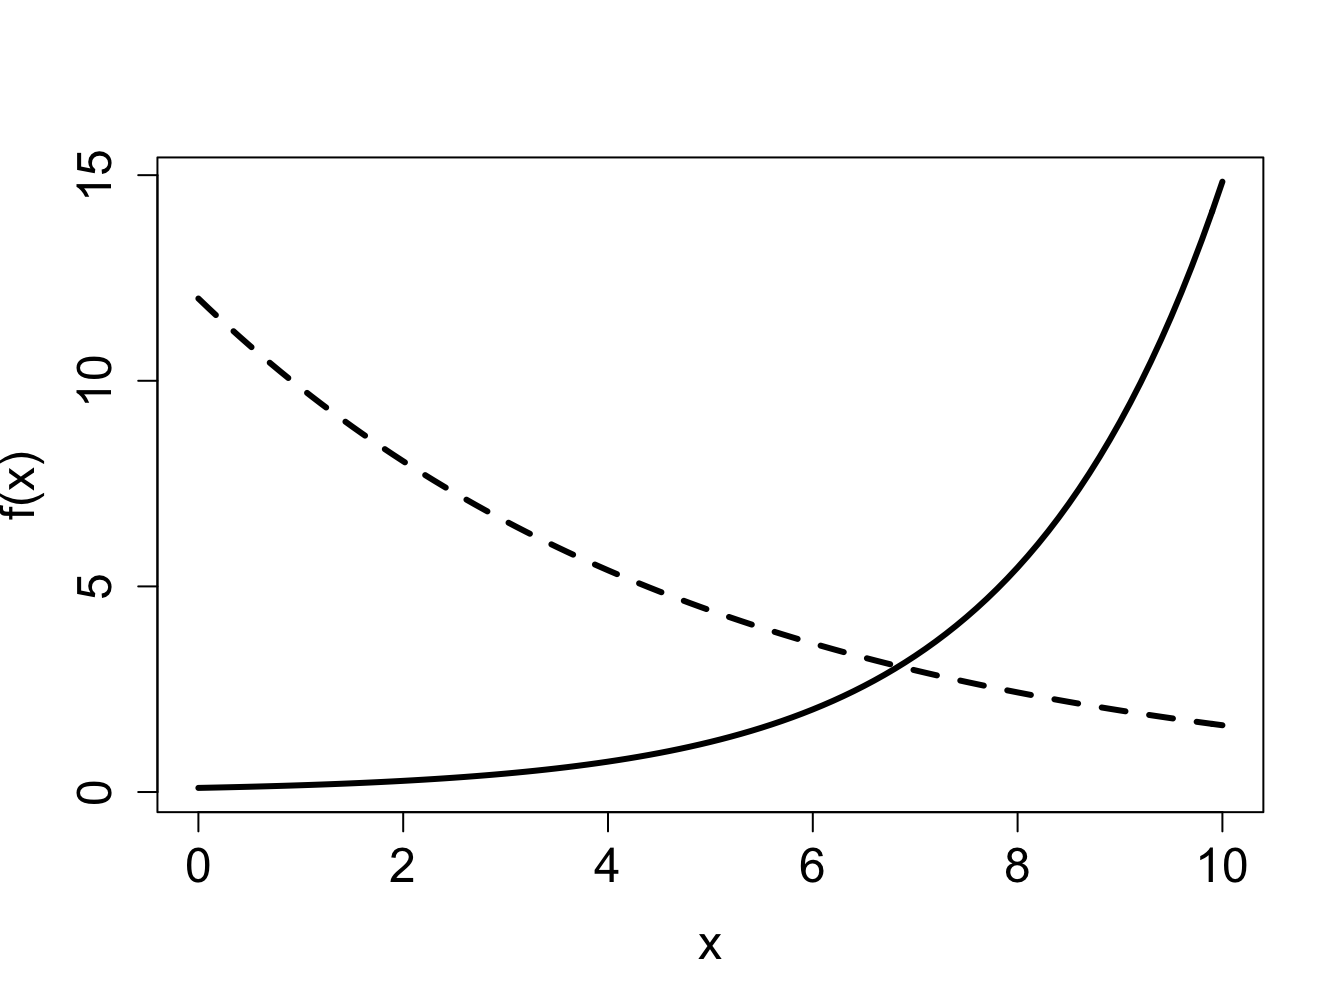
\includegraphics[width=0.5\linewidth]{QuantLife_files/figure-latex/ch2-funk1-2} 

}

\caption{Plots of two linear functions (left) and two exponential functions (right). Can you identify which linear function has the positive slope and which one negative? Which exponential function has a positive rate constant and which one negative?}\label{fig:ch2-funk1}
\end{figure}

\hypertarget{exercises-2}{%
\subsection{Exercises}\label{exercises-2}}

Answer the questions below, some of which refer to the function graphs in figure \ref{ch2-funk1}.

\begin{enumerate}
\def\labelenumi{\arabic{enumi}.}
\item
  Which of the linear graphs in the first figure corresponds to \(f(x) = 5x\) and which corresponds to \(f(x) = 10-x\)? State which parameter allows you to connect the function with its graph and explain why.
\item
  Which of the exponential graphs in the second figure corresponds to \(f(x) = 0.1e^{0.5x}\) and which corresponds to \(f(x) = 12e^{-0.2x}\)? State which parameter allows you to connect the function with its graph and explain why.
\item
  Demonstrate algebraically that a linear function of the form given in equation \ref{eq:linear_funk} satisfies the property of linear functions from definition \ref {def:ch2_linfunk}.
\item
  Demonstrate algebraically that an exponential function of the form given in equation \ref{eq:exp_funk} satisfies the property of exponential functions from definition \ref {def:ch2_expfunk}.
\item
  Modify the exponential function by adding a constant term to it \(f(x) = a e^{rx} + b\). What is is the value of this function at \(x=0\)?
\item
  How does the function defined in the previous exercise, \(f(x) = a e^{rx} + b\), how does it behave as \(x \to \infty\) if \(r>0\)?
\item
  How does the function \(f(x) = a e^{rx} + b\) behave as \(x \to \infty\) if \(r<0\)?
\end{enumerate}

\hypertarget{rational-and-logistic-functions}{%
\subsection{rational and logistic functions}\label{rational-and-logistic-functions}}

Let us now turn to more complex functions, made up of simpler components that we understand. Consider a ratio of two polynomials, called a \index{function!rational} rational function. The general form of such functions can be written down as follows, where ellipsis stands for terms with powers lower than \(n\) or \(m\):
\begin{equation}
 f(x) = \frac{a_0 + ... + a_n x^n}{b_0 + ... + b_m x^m}
\label{eq:rational_funk}
\end{equation}
The two polynomials may have different degrees (highest power of the terms, \(n\) and \(m\)), but they are usually the same in most biological examples. The reason is that if the numerator and the denominator are ``unbalanced'\,', one will inevitably overpower the other for large values of \(x\), which would lead to the function either increasing without bound to infinity (if \(n>m\)) or decaying to zero (if \(m>n\)). There's nothing wrong with that, mathematically, but rational functions are most frequently used to model quantities that approach a nonzero asymptote for large values of the independent variable.

For this reason, let us assume \(m=n\) and consider what happens as \(x \to \infty\). All terms other than the highest-order terms become very small in comparison to \(x^n\) (this is something you can demonstrate to yourself using R), and thus both the numerator and the denominator approach the terms with power \(n\). This can be written using the mathematical limit notation \(\lim_{x \to \infty}\) which describes the value that a function approaches when the independent variable increases without bound:
\[  \lim_{x \to \infty} \frac{a_0 + ... + a_n x^n}{b_0 + ... + b_n x^n} = \frac{ a_n x^n}{ b_n x^n}  =  \frac{ a_n}{ b_n}  \]
Therefore, the function approaches the value of \(a_n /b_n\) as \(x\) grows.

Similarly, let us consider what happens when \(x=0\). Plugging this into the function results in all of the terms vanishing except for the constant terms, so
\[ f(0) =  \frac{ a_0}{ b_0} \]
Between 0 and infinity, the function either increases or decreases monotonically, depending on which value (\(a_n /b_n\) or \(a_0/b_0\)) is greater. Two examples of plots of rational functions are shown in figure \ref{fig:ch2_sigmoidal_plots}, which shows graphs increasing from 0 to 1. Depending on the degree of the polynomials in a rational function, it may increase more gradually (solid line) or more step-like (dashed line).

\textbf{Example.} The following model, called the Hill equation \index{Hill equation}\index{model!Hill}, describes the fraction of receptor molecules which are bound to a ligand, which is a chemical term for a free molecule that binds to another, typically larger, receptor molecule. \(\theta\) is the fraction of receptors bound to a ligand, \(L\) denotes the ligand concentration, \(K_d\) is the dissociation constant, and \(n\) called the binding cooperativity \index{binding cooperativity} or Hill coefficient:
\[ \theta = \frac{L^n}{ L^n +K_d}\]

The Hill equation is a rational function, and Figure \ref{fig:ch2_sigmoidal_plots} shows plots of the graphs of two such function in the right panel. This model is further explored in exercise 2.2.10.

\textbf{Example.} A common model of population over time is the \index{function!logistic} logistic function. There are variations on how it is written down, but here is one general form:
\begin{equation}
 f(x) = \frac{a e^{rx} }{b+e^{rx}}
\label{eq:logistic_funk} 
\end{equation}

The numerator and denominator both contain exponential functions with the same power. If \(r>0\) when \(x \to \infty\), the denominator approaches \(e^{rx}\), since it becomes much greater than \(b\), and we can calculate:
\[  \lim_{x \to \infty}  =  \frac{a e^{rx} }{e^{rx}} = a; \; \mathrm{if} \; r>0 \]

On the other hand, if \(r<0\), then the numerator approaches zero as \(x \to \infty\), and so does the function
\[  \lim_{x \to \infty}  =  \frac{0}{b} = 0; \; \mathrm{if} \; r<0 \]

Notice that switching the sign of \(r\) has the same effect as switching the sign of \(x\), since they are multiplied. Which means that for positive \(r\), if \(x\) is extended to negative infinity, the function approaches 0. This is illustrated in the second plot in Figure \ref{fig:ch2_sigmoidal_plots}, which shows two logistic functions increasing from 0 to a positive level, one with \(a=20\) (solid line) and the second with \(a=10\) (dashed line). The graph of logistic functions has a characteristic \emph{sigmoidal} (S-shaped) shape, and its steepness is determined by the rate \(r\): if \(r\) is small, the curve is soft, if \(r\) is large, the graph resembles a step function.

\begin{figure}

{\centering 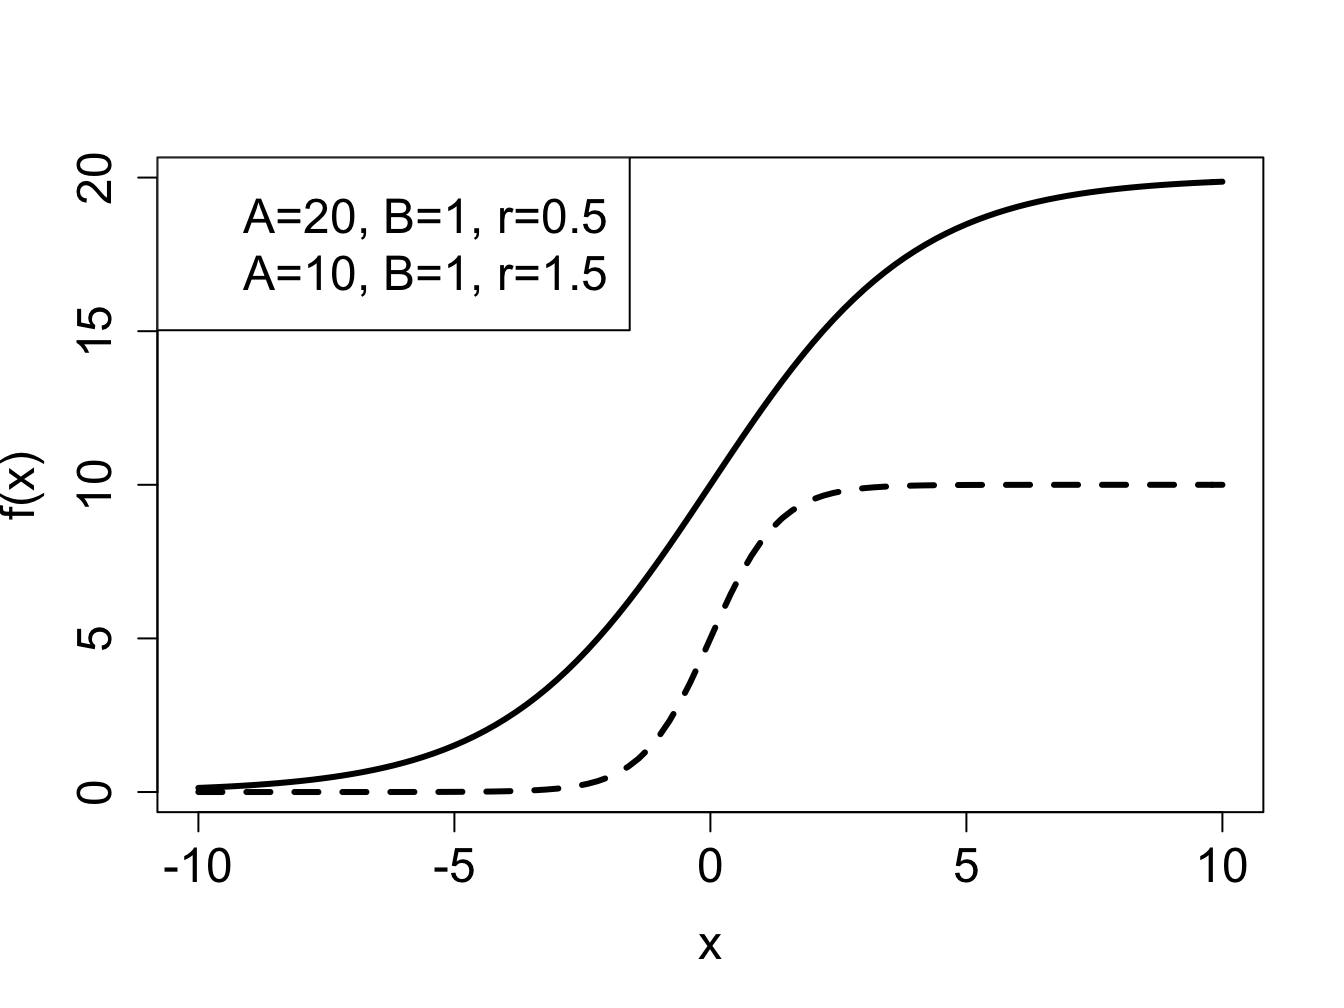
\includegraphics[width=0.5\linewidth]{QuantLife_files/figure-latex/ch2-funk2-1} 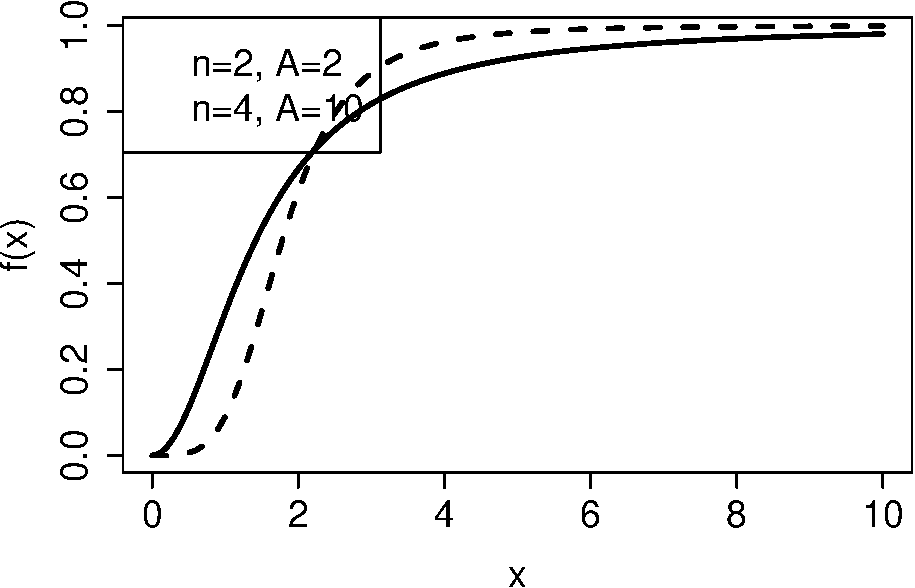
\includegraphics[width=0.5\linewidth]{QuantLife_files/figure-latex/ch2-funk2-2} 

}

\caption{Examples of two graphs of logistic functions (left) and two Hill functions (right).}\label{fig:ch2-funk2}
\end{figure}

\hypertarget{exercises-3}{%
\subsection{Exercises:}\label{exercises-3}}

For each biological model below answer the following questions in terms of the parameters in the models, assuming all are nonnegative real numbers. 1) what is the value of the function when the independent variable is 0? 2) what value does the function approach when the independent variable goes to infinity? 3) verbally describe the behavior of the functions between 0 and infinity (e.g., function increases, decreases).

\begin{enumerate}
\def\labelenumi{\arabic{enumi}.}
\item
  Model of number of mutations \(M\) as a function of time \(t\):
  \[ M(t) = M_0 + \mu t\]
\item
  Model of molecular concentration \(C\) as a function of time \(t\):
  \[ C(t) = C_0 e^{-kt} \]
\item
  Model of cooperative binding of ligands\index{model!binding cooperativity}, with fraction of bound receptors \(\theta\) as a function of ligand concentration \(L\):
  \[ \theta = \frac{L^n}{L^n + K_d}\]
\item
  Model of tree height \(H\) (length) as a function of age \(a\) (time):
  \[ H(a) = \frac{b a }{c + a}\]
\item
  Model of concentration of a gene product \(G\) (concentration) as a function of time \(t\):
  \[ G(t) = G_m (1 - e^{-\alpha t})\]
\item
  The simplified Goldman-Hodgkin-Katz model of ionic current \(I\) (current) as a function of membrane potential \(V\) (voltage):
  \[ I(V) = - b V \frac{1- c e^{-\alpha V}} {1-  e^{-\alpha V}} \]
\item
  Michaelis-Menten model \index{model!Michaelis-Menten} of enzyme kinetics, \(v\) is reaction rate (1/time) and \(S\) is substrate concentration:
  \[ v(S) = \frac{v_{max} S}{K_m + S}\]
\item
  Logistic model \index{logistic model}of population growth, \(P\) is population size and time \(t\):
  \[ P(t) = \frac{A e^{kt}}{1 + B(e^{kt} -1)} \]
\end{enumerate}

\hypertarget{vectors-and-plotting-in-r}{%
\section{Vectors and plotting in R}\label{vectors-and-plotting-in-r}}

\label{sec:comp2}

\hypertarget{writing-scripts-and-calling-functions}{%
\subsection{writing scripts and calling functions}\label{writing-scripts-and-calling-functions}}

Programming means arranging a number of commands in a particular order to perform a task. Typing them one at a time into the command line is inefficient and error-prone. Instead, the commands are written into a file called a program or script (the name depends on the type of language; since R is a scripting language you will be writing scripts), which can be edited, saved, copied, etc. To open a new script file, in R Studio, go to File menu, and choose New R Script. This will open an editor window where you can type your commands. To save the script file (do this often!!), click the Save button (with the little floppy disk icon) or select Save from the File menu. You will also see small buttons at the top of the window that say \texttt{Run}, \texttt{Re-run}, and \texttt{Source}. The first two will run either the current line or a selected region of the script, while the \texttt{Source} button will run the entire file. Now that you know how to create a script, \textbf{you should never type your R code into the command line}, unless you're testing a single command to see what it does, or looking up help.

R comes equipped with many \index{function!in R} \index{R programming!function} functions that correspond to standard mathematical functions. As we saw in section \ref{sec:comp1}, \texttt{exp()} is the exponential function that returns \(e\) raised to the power of the input value. Other common ones are: \texttt{sqrt()} returns the square root of the input value; \texttt{sin()} and \texttt{cos()} return the sine and the cosine of the input value, respectively. Note that all of these function names are followed by parentheses, which is a hallmark of a function (in R as well as in mathematics). This indicates that the input value has to go there, for example \texttt{exp(5)}. To compute the value of \(e^5\), save it into a variable called \texttt{var1} and then print out the value on the screen, you can create the following script:

\begin{Shaded}
\begin{Highlighting}[]
\NormalTok{var1 \textless{}{-}}\StringTok{ }\KeywordTok{exp}\NormalTok{(}\DecValTok{5}\NormalTok{)}
\KeywordTok{print}\NormalTok{(var1)}
\end{Highlighting}
\end{Shaded}

\begin{verbatim}
## [1] 148.4132
\end{verbatim}

If you run the above code chunk in R Studio you will see two things happen: a variable named var1 appears in the Environment window (top right) with the value 148.41\ldots{} and the same value is printed out in the command line window (bottom left).

The most important principle of the procedural brand of programming (which includes R) is this: the computer (that is, the compiler or interpreter) evaluates the commands from top to bottom, one at a time. The variables are used with the values that they are currently assigned. If one variable (\texttt{var1}) was assigned in terms of another (\texttt{var2}), and then \texttt{var2} is changed later, this does not change the value of \texttt{var2}. Here is an illustration of how this works:

\begin{Shaded}
\begin{Highlighting}[]
\NormalTok{var2 \textless{}{-}}\StringTok{ }\DecValTok{20}
\NormalTok{var1 \textless{}{-}}\StringTok{ }\NormalTok{var2}\OperatorTok{/}\DecValTok{20}
\KeywordTok{print}\NormalTok{(var2)}
\end{Highlighting}
\end{Shaded}

\begin{verbatim}
## [1] 20
\end{verbatim}

\begin{Shaded}
\begin{Highlighting}[]
\NormalTok{var2 \textless{}{-}}\StringTok{ }\DecValTok{10}
\KeywordTok{print}\NormalTok{(var1)}
\end{Highlighting}
\end{Shaded}

\begin{verbatim}
## [1] 1
\end{verbatim}

Notice that \texttt{var1} doesn't change, because the R interpreter reads the commands one by one, and does not go back to re-evaluate the assignment for var1 after \texttt{var2} is changed. Learning to think in this methodical, literal manner is crucial for developing programming skills.

\hypertarget{vector-variables}{%
\subsection{vector variables}\label{vector-variables}}

Variables may contain more than a single number, they can also store a bunch of numbers, which is then called an array. When numbers in an array are organized as a single ordered list, this is called a \index{R programming!vector variable}\index{vector!in R} \emph{vector}. There are several ways of producing a vector of numbers in R.

\hypertarget{c-function}{%
\subsubsection{c() function}\label{c-function}}

The most direct method of making a vector is to put together several values by listing them inside the function \texttt{c()} and assigning the output to a variable, e.g.~\texttt{my.vec}:

\begin{Shaded}
\begin{Highlighting}[]
\NormalTok{my.vec\textless{}{-}}\KeywordTok{c}\NormalTok{(pi,}\DecValTok{45}\NormalTok{,}\FloatTok{912.8}\NormalTok{, }\DecValTok{0}\NormalTok{)}
\KeywordTok{print}\NormalTok{(my.vec)}
\end{Highlighting}
\end{Shaded}

\begin{verbatim}
## [1]   3.141593  45.000000 912.800000   0.000000
\end{verbatim}

This variable \texttt{my.vec} is now a vector variable that contains four different numbers. Each of those numbers can be accessed individually by referencing its position in the vector, called the \index{R programming!index of vector} \emph{index}. In the R language the the index for the first number in a vector is 1, the index for the second number is 2, etc. The index is placed in square brackets after the vector name, as follows:

\begin{Shaded}
\begin{Highlighting}[]
\KeywordTok{print}\NormalTok{(my.vec[}\DecValTok{1}\NormalTok{])}
\end{Highlighting}
\end{Shaded}

\begin{verbatim}
## [1] 3.141593
\end{verbatim}

\begin{Shaded}
\begin{Highlighting}[]
\KeywordTok{print}\NormalTok{(my.vec[}\DecValTok{2}\NormalTok{])}
\end{Highlighting}
\end{Shaded}

\begin{verbatim}
## [1] 45
\end{verbatim}

\begin{Shaded}
\begin{Highlighting}[]
\KeywordTok{print}\NormalTok{(my.vec[}\DecValTok{3}\NormalTok{])}
\end{Highlighting}
\end{Shaded}

\begin{verbatim}
## [1] 912.8
\end{verbatim}

\begin{Shaded}
\begin{Highlighting}[]
\KeywordTok{print}\NormalTok{(my.vec[}\DecValTok{4}\NormalTok{])}
\end{Highlighting}
\end{Shaded}

\begin{verbatim}
## [1] 0
\end{verbatim}

\hypertarget{the-colon-operator}{%
\subsubsection{the colon operator}\label{the-colon-operator}}

Another way to generate a sequence of numbers in a particular order is to use the colon operator, which produces a vector of integers from the first number to the last, inclusive. Here are two examples:

\begin{Shaded}
\begin{Highlighting}[]
\NormalTok{my.vec1\textless{}{-}}\DecValTok{1}\OperatorTok{:}\DecValTok{20}
\KeywordTok{print}\NormalTok{(my.vec1)}
\end{Highlighting}
\end{Shaded}

\begin{verbatim}
##  [1]  1  2  3  4  5  6  7  8  9 10 11 12 13 14 15 16 17 18 19 20
\end{verbatim}

\begin{Shaded}
\begin{Highlighting}[]
\NormalTok{my.vec2\textless{}{-}}\DecValTok{0}\OperatorTok{:{-}}\DecValTok{20}
\KeywordTok{print}\NormalTok{(my.vec2)}
\end{Highlighting}
\end{Shaded}

\begin{verbatim}
##  [1]   0  -1  -2  -3  -4  -5  -6  -7  -8  -9 -10 -11 -12 -13 -14 -15 -16 -17 -18
## [20] -19 -20
\end{verbatim}

You can also access some but not all of the values stored in a vector simultaneously. To do this, enter a vector of positive integers inside the square brackets, either using the colon operator or using the \texttt{c()} function. Here are two examples, the first prints out the 4th through the 10th element of the vector \texttt{my.vec1}, while the second prints out the 1st, 5th, and 11th elements of the vector \texttt{my.vec2}:

\begin{Shaded}
\begin{Highlighting}[]
\KeywordTok{print}\NormalTok{(my.vec1[}\DecValTok{4}\OperatorTok{:}\DecValTok{10}\NormalTok{])}
\end{Highlighting}
\end{Shaded}

\begin{verbatim}
## [1]  4  5  6  7  8  9 10
\end{verbatim}

\begin{Shaded}
\begin{Highlighting}[]
\KeywordTok{print}\NormalTok{(my.vec2[}\KeywordTok{c}\NormalTok{(}\DecValTok{1}\NormalTok{,}\DecValTok{5}\NormalTok{,}\DecValTok{11}\NormalTok{)])}
\end{Highlighting}
\end{Shaded}

\begin{verbatim}
## [1]   0  -4 -10
\end{verbatim}

\hypertarget{seq-function}{%
\subsubsection{seq() function}\label{seq-function}}

If you want to generate a sequence of numbers with a constant difference other than 1, you're in luck: R provides a function called \texttt{seq()}. It takes three inputs: the starting value, the ending value, and the step (difference between successive elements). For example, to generate a list of numbers starting at 20 up to 50, with a step size of 3, type the first command; to obtain the same sequence in reverse, use the second command:

\begin{Shaded}
\begin{Highlighting}[]
\NormalTok{my.vec1\textless{}{-}}\KeywordTok{seq}\NormalTok{(}\DecValTok{20}\NormalTok{,}\DecValTok{50}\NormalTok{,}\DecValTok{3}\NormalTok{)}
\KeywordTok{print}\NormalTok{(my.vec1)}
\end{Highlighting}
\end{Shaded}

\begin{verbatim}
##  [1] 20 23 26 29 32 35 38 41 44 47 50
\end{verbatim}

\begin{Shaded}
\begin{Highlighting}[]
\NormalTok{my.vec2\textless{}{-}}\KeywordTok{seq}\NormalTok{(}\DecValTok{50}\NormalTok{,}\DecValTok{20}\NormalTok{,}\OperatorTok{{-}}\DecValTok{3}\NormalTok{)}
\KeywordTok{print}\NormalTok{(my.vec2)}
\end{Highlighting}
\end{Shaded}

\begin{verbatim}
##  [1] 50 47 44 41 38 35 32 29 26 23 20
\end{verbatim}

\hypertarget{rep-function}{%
\subsubsection{rep() function}\label{rep-function}}

Sometimes you want to create a vector of repeated values. For example, you can create a variable with 20 zeros, you can use rep() like this:

\begin{Shaded}
\begin{Highlighting}[]
\NormalTok{zeros \textless{}{-}}\StringTok{ }\KeywordTok{rep}\NormalTok{(}\DecValTok{0}\NormalTok{,}\DecValTok{20}\NormalTok{)}
\KeywordTok{print}\NormalTok{(zeros)}
\end{Highlighting}
\end{Shaded}

\begin{verbatim}
##  [1] 0 0 0 0 0 0 0 0 0 0 0 0 0 0 0 0 0 0 0 0
\end{verbatim}

You can repeat any value, say create a vector by repeating the number pi:

\begin{Shaded}
\begin{Highlighting}[]
\NormalTok{pies \textless{}{-}}\StringTok{ }\KeywordTok{rep}\NormalTok{(pi,}\DecValTok{7}\NormalTok{)}
\KeywordTok{print}\NormalTok{(pies)}
\end{Highlighting}
\end{Shaded}

\begin{verbatim}
## [1] 3.141593 3.141593 3.141593 3.141593 3.141593 3.141593 3.141593
\end{verbatim}

You can even repeat another vector, like the vector my.vec that was assigned above:

\begin{Shaded}
\begin{Highlighting}[]
\NormalTok{my.vecs \textless{}{-}}\StringTok{ }\KeywordTok{rep}\NormalTok{(my.vec, }\DecValTok{5}\NormalTok{)}
\KeywordTok{print}\NormalTok{(my.vecs)}
\end{Highlighting}
\end{Shaded}

\begin{verbatim}
##  [1]   3.141593  45.000000 912.800000   0.000000   3.141593  45.000000
##  [7] 912.800000   0.000000   3.141593  45.000000 912.800000   0.000000
## [13]   3.141593  45.000000 912.800000   0.000000   3.141593  45.000000
## [19] 912.800000   0.000000
\end{verbatim}

\hypertarget{calculations-with-vector-variables}{%
\subsection{calculations with vector variables}\label{calculations-with-vector-variables}}

\begin{Shaded}
\begin{Highlighting}[]
\NormalTok{NewVec \textless{}{-}}\StringTok{ }\DecValTok{2}\OperatorTok{*}\NormalTok{my.vec}
\KeywordTok{print}\NormalTok{(NewVec)}
\end{Highlighting}
\end{Shaded}

\begin{verbatim}
## [1]    6.283185   90.000000 1825.600000    0.000000
\end{verbatim}

You can also perform calculations with multiple vector variables, but this requires extra care. R can perform any arithmetic operation with two vector variables, for instance adding two vectors results in a vector containing the sum of corresponding elements of the two vectors:

\begin{Shaded}
\begin{Highlighting}[]
\NormalTok{my.vec1\textless{}{-}}\DecValTok{1}\OperatorTok{:}\DecValTok{5}
\NormalTok{my.vec2\textless{}{-}}\DecValTok{0}\OperatorTok{:}\DecValTok{4}
\KeywordTok{print}\NormalTok{(my.vec1)}
\end{Highlighting}
\end{Shaded}

\begin{verbatim}
## [1] 1 2 3 4 5
\end{verbatim}

\begin{Shaded}
\begin{Highlighting}[]
\KeywordTok{print}\NormalTok{(my.vec2)}
\end{Highlighting}
\end{Shaded}

\begin{verbatim}
## [1] 0 1 2 3 4
\end{verbatim}

\begin{Shaded}
\begin{Highlighting}[]
\NormalTok{sum.vec\textless{}{-}my.vec1}\OperatorTok{+}\NormalTok{my.vec2}
\KeywordTok{print}\NormalTok{(sum.vec)}
\end{Highlighting}
\end{Shaded}

\begin{verbatim}
## [1] 1 3 5 7 9
\end{verbatim}

One needs to take care that the two vectors have the same number of elements (length). If you try to operate on (e.g.~add) two vectors of different lengths, R will return a warning and the result will not be what you expect:

\begin{Shaded}
\begin{Highlighting}[]
\NormalTok{my.vec1\textless{}{-}}\DecValTok{1}\OperatorTok{:}\DecValTok{2}
\NormalTok{my.vec2\textless{}{-}}\DecValTok{0}\OperatorTok{:}\DecValTok{4}
\KeywordTok{print}\NormalTok{(my.vec1)}
\end{Highlighting}
\end{Shaded}

\begin{verbatim}
## [1] 1 2
\end{verbatim}

\begin{Shaded}
\begin{Highlighting}[]
\KeywordTok{print}\NormalTok{(my.vec2)}
\end{Highlighting}
\end{Shaded}

\begin{verbatim}
## [1] 0 1 2 3 4
\end{verbatim}

\begin{Shaded}
\begin{Highlighting}[]
\NormalTok{sum.vec\textless{}{-}my.vec1}\OperatorTok{+}\NormalTok{my.vec2}
\end{Highlighting}
\end{Shaded}

\begin{verbatim}
## Warning in my.vec1 + my.vec2: longer object length is not a multiple of shorter
## object length
\end{verbatim}

\begin{Shaded}
\begin{Highlighting}[]
\KeywordTok{print}\NormalTok{(sum.vec)}
\end{Highlighting}
\end{Shaded}

\begin{verbatim}
## [1] 1 3 3 5 5
\end{verbatim}

\hypertarget{exercises-4}{%
\subsection{Exercises}\label{exercises-4}}

The following R commands or short scripts contain errors; your job is to fix them so they runs as described.

\begin{enumerate}
\def\labelenumi{\arabic{enumi}.}
\tightlist
\item
  Assign a vector of three numbers to a variable:
\end{enumerate}

\begin{Shaded}
\begin{Highlighting}[]
\NormalTok{date\_num \textless{}{-}}\StringTok{ }\NormalTok{(}\DecValTok{3}\NormalTok{,}\DecValTok{8}\NormalTok{,}\DecValTok{16}\NormalTok{)}
\end{Highlighting}
\end{Shaded}

\begin{enumerate}
\def\labelenumi{\arabic{enumi}.}
\setcounter{enumi}{1}
\tightlist
\item
  Assign a range of values to a vector variable and print out the third one:
\end{enumerate}

\begin{Shaded}
\begin{Highlighting}[]
\NormalTok{the.vals \textless{}{-}}\StringTok{ }\DecValTok{0}\OperatorTok{:}\DecValTok{10}
\NormalTok{print[}\KeywordTok{the.vals}\NormalTok{(}\DecValTok{3}\NormalTok{)]}
\end{Highlighting}
\end{Shaded}

\begin{enumerate}
\def\labelenumi{\arabic{enumi}.}
\setcounter{enumi}{2}
\tightlist
\item
  Assign a range of values to a vector variable and print out the fourtieth and sixty-first values:
\end{enumerate}

\begin{Shaded}
\begin{Highlighting}[]
\NormalTok{all.the.vals \textless{}{-}}\StringTok{ }\DecValTok{0}\OperatorTok{:}\DecValTok{100}
\KeywordTok{print}\NormalTok{(all.the.vals[}\DecValTok{40}\NormalTok{,}\DecValTok{61}\NormalTok{])}
\end{Highlighting}
\end{Shaded}

\begin{enumerate}
\def\labelenumi{\arabic{enumi}.}
\setcounter{enumi}{3}
\tightlist
\item
  Take the two vectors assigned above and assign their product to another vector:
\end{enumerate}

\begin{Shaded}
\begin{Highlighting}[]
\NormalTok{product \textless{}{-}}\StringTok{ }\NormalTok{the.vals}\OperatorTok{*}\NormalTok{all.the.vals}
\end{Highlighting}
\end{Shaded}

\begin{enumerate}
\def\labelenumi{\arabic{enumi}.}
\setcounter{enumi}{4}
\tightlist
\item
  Create a vector vec1 of ten integers and print the second and the eighth elements:
\end{enumerate}

\begin{Shaded}
\begin{Highlighting}[]
\NormalTok{vec1 \textless{}{-}}\StringTok{ }\DecValTok{11}\OperatorTok{:}\DecValTok{20} 
\KeywordTok{print}\NormalTok{(vec1[}\DecValTok{2}\OperatorTok{:}\DecValTok{8}\NormalTok{])}
\end{Highlighting}
\end{Shaded}

\begin{enumerate}
\def\labelenumi{\arabic{enumi}.}
\setcounter{enumi}{5}
\tightlist
\item
  Create a vector \texttt{vec1} and then multiply all of its elements by 20 and assign it to another vector:
\end{enumerate}

\begin{Shaded}
\begin{Highlighting}[]
\NormalTok{vec1\textless{}{-}}\KeywordTok{seq}\NormalTok{(}\OperatorTok{{-}}\DecValTok{3}\NormalTok{,}\DecValTok{2}\NormalTok{,}\FloatTok{0.1}\NormalTok{)}
\NormalTok{vec2 \textless{}{-}}\StringTok{ }\NormalTok{20vec1}
\end{Highlighting}
\end{Shaded}

\begin{enumerate}
\def\labelenumi{\arabic{enumi}.}
\setcounter{enumi}{6}
\tightlist
\item
  Create a vector \texttt{vec1}, a vector \texttt{vec2} and print out all the elements of the first divided by the second:
\end{enumerate}

\begin{Shaded}
\begin{Highlighting}[]
\NormalTok{vec1 \textless{}{-}}\StringTok{ }\DecValTok{0}\OperatorTok{:}\DecValTok{5}
\NormalTok{vec2 \textless{}{-}}\StringTok{ }\DecValTok{3}\OperatorTok{:}\DecValTok{8}
\NormalTok{print[vec1}\OperatorTok{/}\NormalTok{vec2]}
\end{Highlighting}
\end{Shaded}

\hypertarget{plotting-with-vectors}{%
\subsection{Plotting with vectors}\label{plotting-with-vectors}}

\begin{Shaded}
\begin{Highlighting}[]
\KeywordTok{curve}\NormalTok{(x}\OperatorTok{\^{}}\DecValTok{2}\NormalTok{, }\DecValTok{0}\NormalTok{, }\DecValTok{10}\NormalTok{, }\DataTypeTok{lwd =} \DecValTok{3}\NormalTok{, }\DataTypeTok{xlab =} \StringTok{"x"}\NormalTok{, }\DataTypeTok{ylab =} \StringTok{"quadratic"}\NormalTok{, }
    \DataTypeTok{cex.axis =} \FloatTok{1.5}\NormalTok{, }\DataTypeTok{cex.lab =} \FloatTok{1.5}\NormalTok{)}
\KeywordTok{curve}\NormalTok{(}\DecValTok{20} \OperatorTok{*}\StringTok{ }\KeywordTok{exp}\NormalTok{(}\OperatorTok{{-}}\FloatTok{0.5} \OperatorTok{*}\StringTok{ }\NormalTok{x), }\DecValTok{0}\NormalTok{, }\DecValTok{5}\NormalTok{, }\DataTypeTok{lwd =} \DecValTok{3}\NormalTok{, }\DataTypeTok{xlab =} \StringTok{"x"}\NormalTok{, }
    \DataTypeTok{ylab =} \StringTok{"exponential"}\NormalTok{, }\DataTypeTok{cex.axis =} \FloatTok{1.5}\NormalTok{, }\DataTypeTok{cex.lab =} \FloatTok{1.5}\NormalTok{)}
\end{Highlighting}
\end{Shaded}

\begin{figure}

{\centering 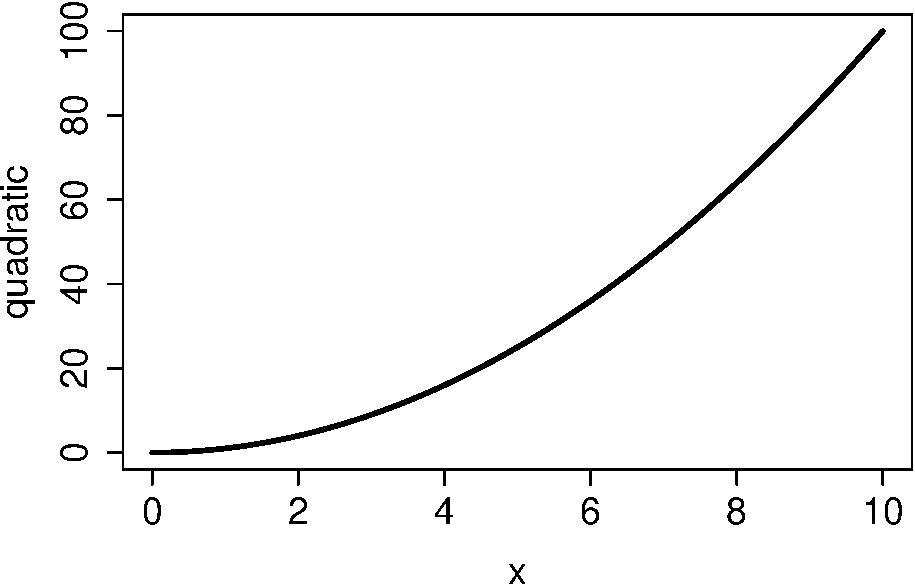
\includegraphics[width=0.5\linewidth]{QuantLife_files/figure-latex/ch2-plot1-1} 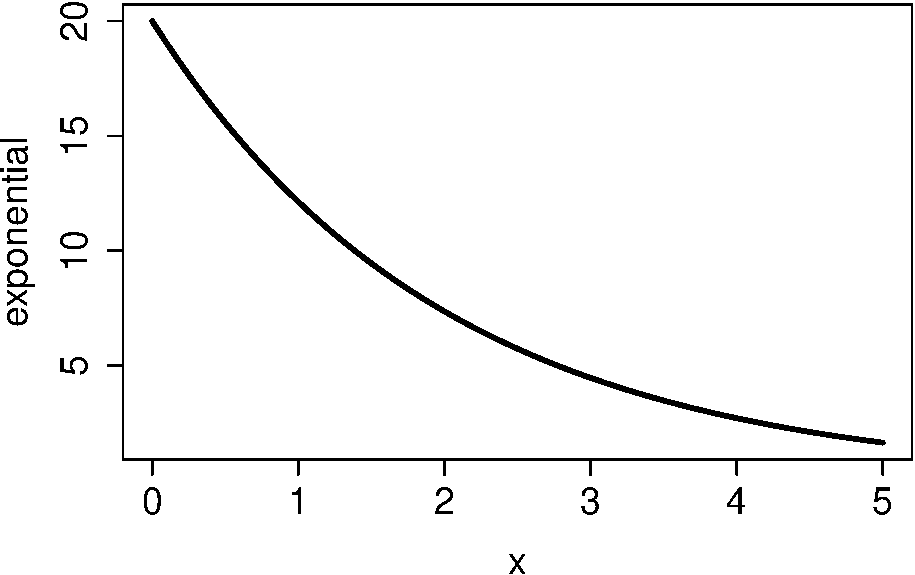
\includegraphics[width=0.5\linewidth]{QuantLife_files/figure-latex/ch2-plot1-2} 

}

\caption{Two examples of plots using curve: quadratic ($y=x^2$) and exponential ($y=20*e^{-0.5x}$)}\label{fig:ch2-plot1}
\end{figure}

There are several ways of \index{plot!in R} \index{R programming!plotting} creating plots of mathematical functions or data R. If you want to plot a mathematical function, the simplest function is \texttt{curve()}. You can tell that this is a function, because it uses parentheses; the first input is an expression for the function, and the next two define the range of the independent variable over which to plot the graph. Two examples of plotting a quadratic function over the range from 0 and 5, and an exponential variation over the range of 0 to 10 are shown in figure \ref{fig:ch2-plot1}.

One can change the default look of the plot produced by curve by setting different options, which are optional inputs into the curve function, One is the line width \texttt{lwd} which can be increased from the default value of 1 to produce thicker curves, as demonstrated in the example above. One can add labels on the x and y axes with \texttt{xlab} and \texttt{ylab} options, respectively; note that these are strings of characters, and thus must be put in quotes to differentiate them from a variable name. There is one very important option not shown above: that of overlaying a curve on top of an existing plot, which is done by typing \texttt{add=TRUE}. This option takes logical (Boolean) values \texttt{TRUE} and \texttt{FALSE}, which must be typed in all caps and without quotes.

\hypertarget{plot-function}{%
\subsubsection{plot() function}\label{plot-function}}

In addition to curve, one can use the function \texttt{plot()} in R to create two dimensional graphs from two vector-valued variables of the same length, e.g.~\texttt{plot(x,y)}. The first input variable corresponds to the \index{variable!independent} \emph{independent variable} (e.g.~\texttt{x}), which is plotted on the x-axis, and the second variable corresponds to the \index{variable!dependent} \emph{dependent variable} (e.g.~\texttt{y}) which is plotted on the y-axis. In figure \ref{fig:ch2-plot2} you see graphs of exponential and logistic function plotted using \texttt{plot()}.

The following chunk creates a vector variable time, then calculates a new variable quad using time in a single operation:

\begin{Shaded}
\begin{Highlighting}[]
\NormalTok{time \textless{}{-}}\StringTok{ }\DecValTok{0}\OperatorTok{:}\DecValTok{10}
\NormalTok{quad \textless{}{-}}\StringTok{ }\NormalTok{(time }\OperatorTok{{-}}\StringTok{ }\DecValTok{5}\NormalTok{)}\OperatorTok{\^{}}\DecValTok{2}
\KeywordTok{print}\NormalTok{(time)}
\end{Highlighting}
\end{Shaded}

\begin{verbatim}
##  [1]  0  1  2  3  4  5  6  7  8  9 10
\end{verbatim}

\begin{Shaded}
\begin{Highlighting}[]
\KeywordTok{print}\NormalTok{(quad)}
\end{Highlighting}
\end{Shaded}

\begin{verbatim}
##  [1] 25 16  9  4  1  0  1  4  9 16 25
\end{verbatim}

This chunk plots the two vector variables quad as a function of time, and adds a title to the plot

\begin{Shaded}
\begin{Highlighting}[]
\KeywordTok{plot}\NormalTok{(time, quad, }\DataTypeTok{main =} \StringTok{"Quadratic function of time"}\NormalTok{)}
\end{Highlighting}
\end{Shaded}

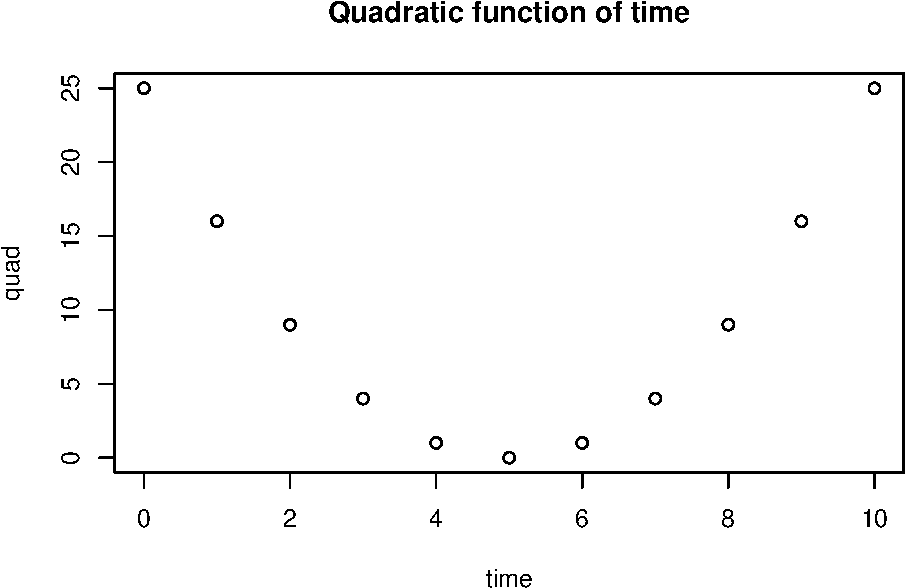
\includegraphics{QuantLife_files/figure-latex/unnamed-chunk-44-1.pdf}

The default plot style in R uses circles to indicate each plotted point. To change it, you need to set the option \texttt{t} (type), for example, setting \texttt{t=\textquotesingle{}l\textquotesingle{}} (the lowercase letter L) produces a continuous line connecting the individual data points.

\begin{Shaded}
\begin{Highlighting}[]
\KeywordTok{plot}\NormalTok{(time, quad, }\DataTypeTok{main =} \StringTok{"Quadratic function of time"}\NormalTok{, }\DataTypeTok{type =} \StringTok{"l"}\NormalTok{, }\DataTypeTok{xlab =} \StringTok{"time"}\NormalTok{, }
    \DataTypeTok{ylab =} \StringTok{"y = f(t)"}\NormalTok{)}
\end{Highlighting}
\end{Shaded}

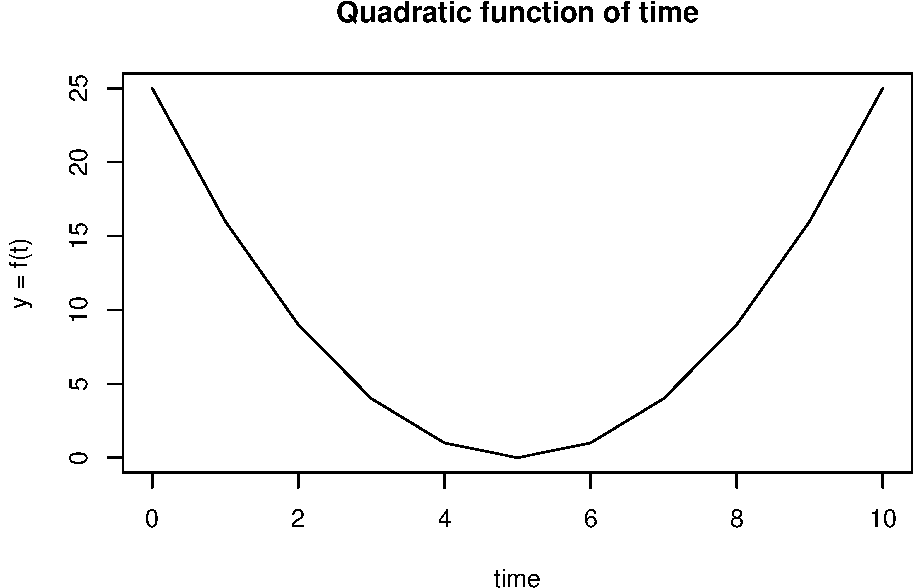
\includegraphics{QuantLife_files/figure-latex/unnamed-chunk-45-1.pdf}

\texttt{plot()} is a versatile function that has many options function has many options which can be changed to determine the color, the style, and other attributes of the plot. For a full list type \texttt{help(plot)} in the console or type plot in the search bar of the Help pane in the bottom right window.

\hypertarget{using-lines-or-points}{%
\subsubsection{using lines() or points()}\label{using-lines-or-points}}

You may also want to plot multiple graphs on the same figure. The \texttt{plot()} function creates a new plot window, so if you want to add another plot on top of the first one, you have to use another function. There are two ones available: \texttt{lines()} which produces continuous curves connecting the points, and \texttt{points()} which plots individual symbols at every point.

Let us illustrate this by plotting two different exponential functions on one plot, and two different logistic functions on the second one, which were discussed in section \ref{sec:math2}. When you've got multiple plots on the same figure, they need to be distinct and labeled. To distinguish them, below I use the option \texttt{col} to specify the color of the plot, and I add a legend describing the parameters of each plot to the figure \ref{fig:ch2-plot2}. The function has a lot of options, so if you want to understand the details, type \texttt{help(legend)} in the prompt or go to Help tab in the lower right frame of R Studio and type legend.

\begin{Shaded}
\begin{Highlighting}[]
\NormalTok{x \textless{}{-}}\StringTok{ }\KeywordTok{seq}\NormalTok{(}\DecValTok{0}\NormalTok{, }\DecValTok{10}\NormalTok{, }\FloatTok{0.5}\NormalTok{)}
\NormalTok{y \textless{}{-}}\StringTok{ }\DecValTok{10} \OperatorTok{+}\StringTok{ }\DecValTok{20} \OperatorTok{*}\StringTok{ }\KeywordTok{exp}\NormalTok{(}\OperatorTok{{-}}\FloatTok{0.5} \OperatorTok{*}\StringTok{ }\NormalTok{x)}
\KeywordTok{plot}\NormalTok{(x, y, }\DataTypeTok{xlab =} \StringTok{"x"}\NormalTok{, }\DataTypeTok{ylab =} \StringTok{"exponential"}\NormalTok{, }\DataTypeTok{col =} \DecValTok{1}\NormalTok{, }\DataTypeTok{lwd =} \DecValTok{3}\NormalTok{)}
\NormalTok{y \textless{}{-}}\StringTok{ }\DecValTok{10} \OperatorTok{+}\StringTok{ }\DecValTok{20} \OperatorTok{*}\StringTok{ }\KeywordTok{exp}\NormalTok{(}\OperatorTok{{-}}\DecValTok{2} \OperatorTok{*}\StringTok{ }\NormalTok{x)}
\KeywordTok{lines}\NormalTok{(x, y, }\DataTypeTok{col =} \DecValTok{2}\NormalTok{, }\DataTypeTok{lwd =} \DecValTok{3}\NormalTok{)}
\NormalTok{leg.txt =}\StringTok{ }\KeywordTok{c}\NormalTok{(}\StringTok{"b=10,a=20,r={-}0.5"}\NormalTok{, }\StringTok{"b=10,a=20,r={-}2"}\NormalTok{)}
\KeywordTok{legend}\NormalTok{(}\StringTok{"topright"}\NormalTok{, leg.txt, }\DataTypeTok{col =} \DecValTok{1}\OperatorTok{:}\DecValTok{2}\NormalTok{, }\DataTypeTok{pch =} \KeywordTok{c}\NormalTok{(}\DecValTok{1}\NormalTok{, }\OtherTok{NA}\NormalTok{), }\DataTypeTok{lty =} \KeywordTok{c}\NormalTok{(}\DecValTok{0}\NormalTok{, }\DecValTok{1}\NormalTok{), }\DataTypeTok{lwd =} \DecValTok{3}\NormalTok{)}
\NormalTok{x \textless{}{-}}\StringTok{ }\KeywordTok{seq}\NormalTok{(}\OperatorTok{{-}}\DecValTok{10}\NormalTok{, }\DecValTok{10}\NormalTok{, }\DecValTok{1}\NormalTok{)}
\NormalTok{y \textless{}{-}}\StringTok{ }\DecValTok{20} \OperatorTok{*}\StringTok{ }\KeywordTok{exp}\NormalTok{(}\FloatTok{0.5} \OperatorTok{*}\StringTok{ }\NormalTok{x)}\OperatorTok{/}\NormalTok{(}\DecValTok{1} \OperatorTok{+}\StringTok{ }\KeywordTok{exp}\NormalTok{(}\FloatTok{0.5} \OperatorTok{*}\StringTok{ }\NormalTok{x))}
\KeywordTok{plot}\NormalTok{(x, y, }\DataTypeTok{xlab =} \StringTok{"x"}\NormalTok{, }\DataTypeTok{ylab =} \StringTok{"logistic"}\NormalTok{, }\DataTypeTok{col =} \DecValTok{4}\NormalTok{, }\DataTypeTok{lwd =} \DecValTok{3}\NormalTok{)}
\NormalTok{y \textless{}{-}}\StringTok{ }\DecValTok{20} \OperatorTok{*}\StringTok{ }\KeywordTok{exp}\NormalTok{(}\FloatTok{1.5} \OperatorTok{*}\StringTok{ }\NormalTok{x)}\OperatorTok{/}\NormalTok{(}\DecValTok{1} \OperatorTok{+}\StringTok{ }\KeywordTok{exp}\NormalTok{(}\FloatTok{1.5} \OperatorTok{*}\StringTok{ }\NormalTok{x))}
\KeywordTok{lines}\NormalTok{(x, y, }\DataTypeTok{col =} \DecValTok{2}\NormalTok{, }\DataTypeTok{lwd =} \DecValTok{3}\NormalTok{)}
\NormalTok{leg.txt =}\StringTok{ }\KeywordTok{c}\NormalTok{(}\StringTok{"a=20,b=1,r=0.5"}\NormalTok{, }\StringTok{"a=20,b=1,r=1.5"}\NormalTok{)}
\KeywordTok{legend}\NormalTok{(}\StringTok{"topleft"}\NormalTok{, leg.txt, }\DataTypeTok{col =} \KeywordTok{c}\NormalTok{(}\DecValTok{4}\NormalTok{, }\DecValTok{2}\NormalTok{), }\DataTypeTok{pch =} \KeywordTok{c}\NormalTok{(}\DecValTok{1}\NormalTok{, }\OtherTok{NA}\NormalTok{), }\DataTypeTok{lty =} \KeywordTok{c}\NormalTok{(}\DecValTok{0}\NormalTok{, }\DecValTok{1}\NormalTok{), }\DataTypeTok{lwd =} \DecValTok{3}\NormalTok{)}
\end{Highlighting}
\end{Shaded}

\begin{figure}

{\centering 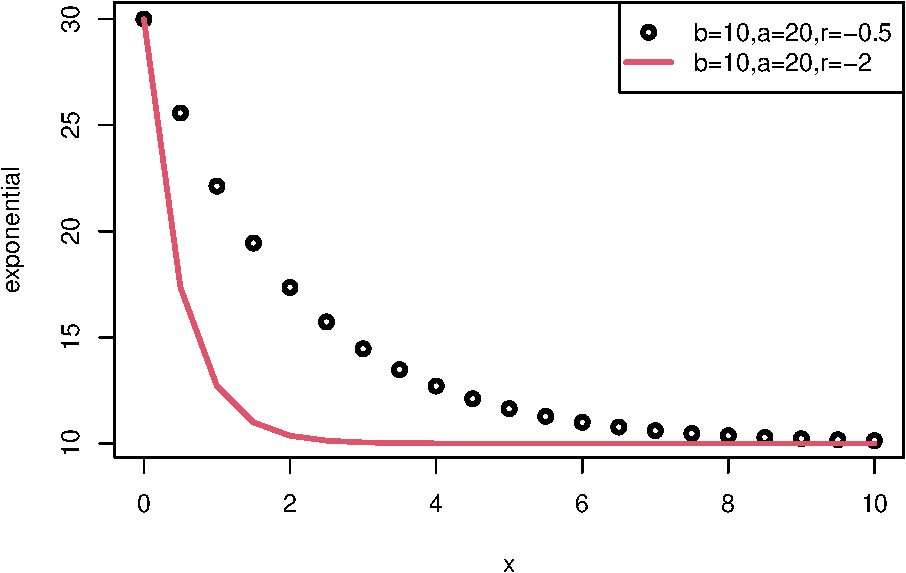
\includegraphics[width=0.5\linewidth]{QuantLife_files/figure-latex/ch2-plot2-1} 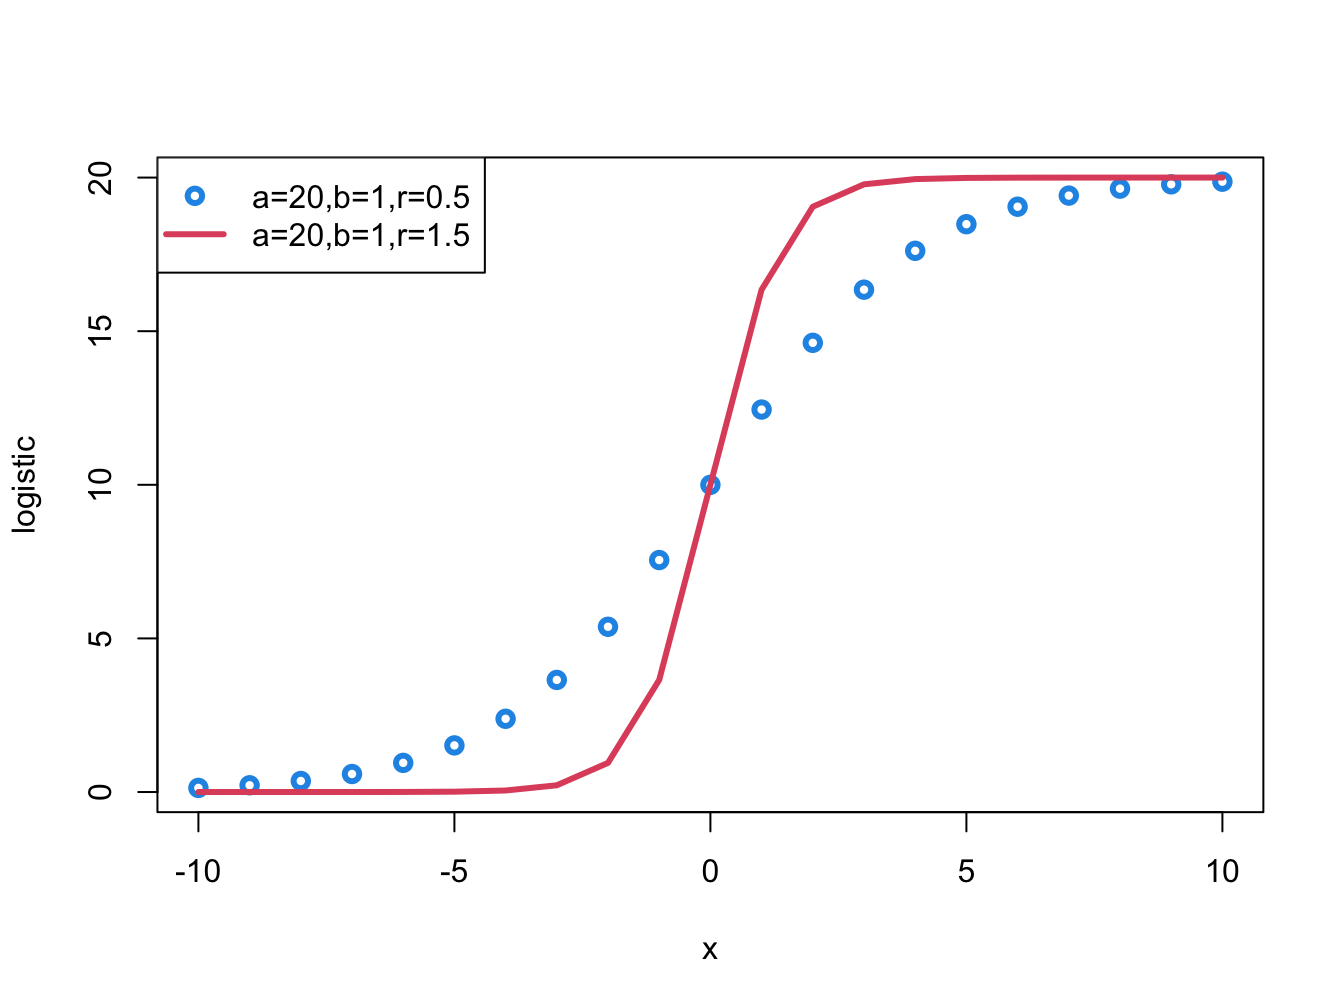
\includegraphics[width=0.5\linewidth]{QuantLife_files/figure-latex/ch2-plot2-2} 

}

\caption{Overlaying multiple plots in R: two exponential functions of the form $y=b+ae^{rx}$ on the left, two logistic functions of the form $y= ae^{rx}/(b+e^{rx})$ on the right.}\label{fig:ch2-plot2}
\end{figure}

\hypertarget{exercises-5}{%
\subsection{Exercises}\label{exercises-5}}

The following R commands or short scripts contain errors; your job is to fix them so they runs as described.

\begin{enumerate}
\def\labelenumi{\arabic{enumi}.}
\tightlist
\item
  Multiply a vector by a constant and add another constant and assign the result to a vector:
\end{enumerate}

\begin{Shaded}
\begin{Highlighting}[]
\NormalTok{new.vals \textless{}{-}}\StringTok{ }\DecValTok{5} \OperatorTok{+}\StringTok{ }\NormalTok{8the.vals}
\end{Highlighting}
\end{Shaded}

\begin{enumerate}
\def\labelenumi{\arabic{enumi}.}
\setcounter{enumi}{1}
\tightlist
\item
  Assign range to be a sequence of values from 0 to 100 with step of 0.1, and calculate the vector variable result as the square of the vector variable range:
\end{enumerate}

\begin{Shaded}
\begin{Highlighting}[]
\NormalTok{range \textless{}{-}}\StringTok{ }\KeywordTok{seq}\NormalTok{(}\DecValTok{0}\NormalTok{,}\FloatTok{0.1}\NormalTok{,}\DecValTok{100}\NormalTok{)}
\NormalTok{result \textless{}{-}}\StringTok{ }\KeywordTok{square}\NormalTok{(range)}
\end{Highlighting}
\end{Shaded}

\begin{enumerate}
\def\labelenumi{\arabic{enumi}.}
\setcounter{enumi}{2}
\tightlist
\item
  Plot result as a function of range:
\end{enumerate}

\begin{Shaded}
\begin{Highlighting}[]
\KeywordTok{plot}\NormalTok{(result, range)}
\end{Highlighting}
\end{Shaded}

\begin{enumerate}
\def\labelenumi{\arabic{enumi}.}
\setcounter{enumi}{3}
\tightlist
\item
  Plot the graph of the function \(f(x) = (45-x)/(4x+3)\) over the range of 0 to 100:
\end{enumerate}

\begin{Shaded}
\begin{Highlighting}[]
\KeywordTok{curve}\NormalTok{((}\DecValTok{45}\OperatorTok{{-}}\NormalTok{x)}\OperatorTok{/}\NormalTok{(4x}\OperatorTok{+}\DecValTok{3}\NormalTok{), }\DecValTok{0}\NormalTok{, }\DecValTok{100}\NormalTok{)}
\end{Highlighting}
\end{Shaded}

\begin{enumerate}
\def\labelenumi{\arabic{enumi}.}
\setcounter{enumi}{4}
\tightlist
\item
  Plot a quadratic function with specified coefficients \(a\), \(b\), \(c\) over a given range of independent variable \(x\):
\end{enumerate}

\begin{Shaded}
\begin{Highlighting}[]
\NormalTok{a\textless{}{-}}\DecValTok{10}
\NormalTok{b\textless{}{-}}\StringTok{ }\DecValTok{{-}15}
\NormalTok{c\textless{}{-}}\StringTok{ }\DecValTok{5}
\NormalTok{y\textless{}{-}a}\OperatorTok{*}\NormalTok{x}\OperatorTok{\^{}}\DecValTok{2}\OperatorTok{+}\NormalTok{b}\OperatorTok{*}\NormalTok{x}\OperatorTok{+}\NormalTok{c}
\NormalTok{x\textless{}{-}}\KeywordTok{seq}\NormalTok{(}\OperatorTok{{-}}\FloatTok{0.5}\NormalTok{,}\DecValTok{2}\NormalTok{,}\FloatTok{0.01}\NormalTok{) }
\KeywordTok{plot}\NormalTok{(x,y,}\DataTypeTok{type=}\StringTok{\textquotesingle{}l\textquotesingle{}}\NormalTok{)}
\end{Highlighting}
\end{Shaded}

\begin{enumerate}
\def\labelenumi{\arabic{enumi}.}
\setcounter{enumi}{5}
\tightlist
\item
  Overlay two different plots of the logistic function with different values of the parameter \(r\):
\end{enumerate}

\begin{Shaded}
\begin{Highlighting}[]
\NormalTok{time\textless{}{-}}\DecValTok{0}\OperatorTok{:}\DecValTok{100}
\NormalTok{a\textless{}{-}}\DecValTok{1000}
\NormalTok{b\textless{}{-}}\DecValTok{50} 
\NormalTok{r\textless{}{-}}\FloatTok{0.1}
\NormalTok{Population\textless{}{-}a}\OperatorTok{*}\KeywordTok{exp}\NormalTok{(r}\OperatorTok{*}\NormalTok{time)}\OperatorTok{/}\NormalTok{(b}\OperatorTok{+}\KeywordTok{exp}\NormalTok{(r}\OperatorTok{*}\NormalTok{time)) }
\KeywordTok{plot}\NormalTok{(time,Population,}\DataTypeTok{type=}\StringTok{\textquotesingle{}l\textquotesingle{}}\NormalTok{) }
\NormalTok{r\textless{}{-}}\DecValTok{10} 
\KeywordTok{lines}\NormalTok{(time,Population,}\DataTypeTok{col=}\DecValTok{2}\NormalTok{)}
\end{Highlighting}
\end{Shaded}

\hypertarget{rates-of-biochemical-reactions}{%
\section{Rates of biochemical reactions}\label{rates-of-biochemical-reactions}}

\label{sec:bio2}

Living things are dynamic, they change with time, and much of mathematical modeling in biology is interested in describing these changes. Some quantities change fast and others slowly, and every dynamic quantity has a rate of change, or \emph{rate} for short. Usually, the quantity that we want to track over time is the variable, and in order to describe how it changes we introduce a rate parameter. If we are describing changes over time, all rate parameters have dimensions with time in the denominator. As a simple example, the velocity of a physical object describes the change in distance over time, so its dimension is \([v] = length/time\).

On the most fundamental level, the work of life is performed by molecules. The protein hemoglobin transports oxygen in the red blood cells, while neurotransmitter molecules like serotonin carry signals between neurons. Enzymes catalyze reactions, like those involved in oxidizing sugar and making ATP, the energy currency of life. Various molecules bind to DNA to turn genes on and off, while myosin proteins walk along actin fibers to create muscle contractions.

In order to describe the activity of biological molecules, we must measure and quantify them. However, they are so small and so numerous that it is not usually practical to count individual molecules (although with modern experimental techniques it is sometimes possible). Instead, biologists describe their numbers using concentrations. Concentration has dimensions of number of molecules per volume, and the units are typically molarity, or moles (\(\approx 6.022*10^{23}\) molecules) per liter. Using concentrations to describe molecule rests on the assumption that there are many molecules and they are well-mixed, or homogeneously distributed throughout the volume of interest.

Molecular reactions are essential for biology, whether they happen inside a bacterial cell or in the bloodstream of a human. \emph{Reaction kinetics} \index{kinetics!reaction} refers to the description of the rates, or the speed, of chemical reactions. Different reactions occur with different rates, which may be dependent on the concentration of the reactant molecule. Consider a simple reaction of molecule \(A\) (called the substrate) turning into molecule \(B\) (called the product), which is usually written by chemists with an arrow:
\[
  A \xrightarrow{k} B
\]
But how fast does the reaction take place? To write down a mathematical model, we need to define the quantities involved. First, we have the concentration of the molecule \(A\), with dimensions of concentration. Second, we have the rate of reaction, let us call it \(v\), which has dimension of concentration per time (just like velocity is length per time). How are the two quantities related?

\hypertarget{constant-zeroth-order-kinetics}{%
\subsection{Constant (zeroth-order) kinetics}\label{constant-zeroth-order-kinetics}}

\index{kinetics!zeroth-order} In some circumstances, the reaction rate \(v\) does not depend on the concentration of the reactant molecule \(A\). In that case, the relationship between the \index{kinetics!rate constant} \emph{rate constant} \(k\) and the actual rate \(v\) is:
\begin{equation}
v = k
\label{eq:kinetics_0th_order}
\end{equation}

Dimensional analysis insists that the dimension of \(k\) must be the dimension of \(v\), or concentration/time. This is known as constant, or zero-order kinetics, and it is observed at concentrations of \(A\) when the reaction is at its maximum velocity: for example, ethanol metabolism by ethanol dehydrogenase in human liver cannot proceed any faster than about 1 drink per hour.

\hypertarget{first-order-kinetics}{%
\subsection{First-order kinetics}\label{first-order-kinetics}}

\index{kinetics!first-order}. In other conditions, it is easy to imagine that increasing the concentration of the reactant \(A\) will speed up the rate of the reaction. A simple relationship of this type is linear:
\begin{equation}
v = kA
\label{eq:kinetics_1st_order}
\end{equation}

In this case, the dimension of the rate constant \(k\) is 1/time. This is called first-order kinetics, and it usually describes reactions when the concentration of \(A\) is small, and there are plenty of free enzymes to catalyze more reactions.

\hypertarget{michaelis-menten-model-of-enzyme-kinetics}{%
\subsection{\texorpdfstring{Michaelis-Menten model of enzyme kinetics \index{kinetics!Michaelis-Menten}}{Michaelis-Menten model of enzyme kinetics }}\label{michaelis-menten-model-of-enzyme-kinetics}}

However, if the concentration of the substrate molecule \(A\) is neither small nor large, we need to consider a more sophisticated model. An enzyme is a protein which catalyzes a biochemical reaction, and it works in two steps: first it binds the substrate, at which point it can still dissociate and float away, and then it actually catalyzes the reaction, which is usually practically irreversible (at least by this enzyme) and releases the product. The enzyme itself is not affected or spent, so it is free to catalyze more reactions. Let denote the substrate (reactant) molecule by \(A\), the product molecule by \(B\), the enzyme by \(E\), and the complex of substrate and enzyme \(AE\). The classic chemical scheme that describes these reactions is this:
\[
A + E \underset{k_{-1}}{\overset{k_1}{\rightleftharpoons}} AE  \xrightarrow{k_2} E + B
\]

You could write three different kinetic equations for the three different arrows in that scheme. Michaelis and Menten used the simplifying assumptions that the binding and dissociation happens much faster than the catalytic reaction, and based on this they were able to write down an approximate, but extremely useful Michaelis-Menten model of an enzymatic reaction:
\begin{equation}
v = \frac{v_{max} A}{K_M+A}
\label{eq:kinetics_MM_kinetics}
\end{equation}
Here \(v\) refers to the rate of the entire catalytic process, that is, the rate of production of \(B\), rather than any intermediate step. Here the reaction rate depends both on the concentration of the substrate \(A\) and on the two constants \(v_{max}\), called the maximum reaction rate, and the constant \(K_M\), called the Michaelis constant. They both depend on the rate constants of the reaction, and \(v_{max}\) also depends on the concentration of the enzyme. The details of the derivation are beyond us for now, but you will see in the following exercises how this model behaves for different values of \(A\).

\%Make a box?
\%Chemical kinetics models are important in a variety of biological fields. The concentration of a drug in the bloodstream is described by an equation that involves the rate of application of the drug and the rate of its removal, known as drug metabolism. The concentration of a sugar, such as fructose, in a cell an be modeled as a system of differential equations that describe all the reactions in the process of glycolysis. Many important molecules exist primarily to regulate each other, for instance, the product of a gene (the protein which is produced when the gene is expressed) can be used to turn on another gene, whose product may turn off the first gene. Such networks of interactions can also be described by a bunch of kinetics equations; the growing field of systems biology studies their complex behaviors.

\hypertarget{r-assignment-1}{%
\section{R Assignment}\label{r-assignment-1}}

\begin{enumerate}
\def\labelenumi{\arabic{enumi}.}
\tightlist
\item
  Copy your script from the R assignment in chapter 1, question 1 and modify the line that assigns the time variable to instead assign it a vector from 0 to 1440 minutes (one for each minute); keep the same values for stroke volume and heart rate. Then your calculation for total volume should produce a vector of the same length as time. Print out the value of the vector after 3 hours (72 minutes), keeping in mind that it is the 73rd element of the vector. ANSWER: 324000 ml
\end{enumerate}

\begin{Shaded}
\begin{Highlighting}[]
\CommentTok{\# THIS IS A COMMENT. YOUR CODE GOES HERE }
\end{Highlighting}
\end{Shaded}

Plot the volume vs time using the type line with black line color and label your axes. Then change the heart rate to 120 beats per minute and re-calculate the total blood volume with the new parmamer. Overlay that plot on top of the previous one using the lines() funcion with red line color. Based on the plots, describe what kind of function is this model, and what is the graphical difference between the two graphs.

\begin{Shaded}
\begin{Highlighting}[]
\CommentTok{\# THIS IS A COMMENT. YOUR CODE GOES HERE }
\end{Highlighting}
\end{Shaded}

TYPE YOUR ANSWERS HERE

\begin{enumerate}
\def\labelenumi{\arabic{enumi}.}
\setcounter{enumi}{1}
\tightlist
\item
  Copy your script from the R assignment in chapter 1, question 2 and modify the line that assigns the time variable to instead assign it a vector from 0 to 60 days (one for each day); keep the same values for all the other variables. Then your calculation for total number of infected should produce a vector of the same length as time. Print out the value of the vector after 10 days, keeping in mind that it is the 11th element of the vector. ANSWER: 43.1785 infected
\end{enumerate}

\begin{Shaded}
\begin{Highlighting}[]
\CommentTok{\# THIS IS A COMMENT. YOUR CODE GOES HERE }
\end{Highlighting}
\end{Shaded}

Plot the total infected population vs time using the type line with black line color and label your axes. Then change the infection rate to 10\% and recalculate the infection numbers with the new parameter. Overlay that plot on top of the previous one using the lines() function with red line color. Based on the plots, report what are the \emph{approximate} doubling times for the number of infectious for the two different infection rates.

\begin{Shaded}
\begin{Highlighting}[]
\CommentTok{\# THIS IS A COMMENT. YOUR CODE GOES HERE }
\end{Highlighting}
\end{Shaded}

TYPE YOUR ANSWERS HERE

\begin{enumerate}
\def\labelenumi{\arabic{enumi}.}
\setcounter{enumi}{2}
\tightlist
\item
  Copy your script from the R assignment in chapter 1, question 3 and modify the line that assigns the time variable to instead assign it a vector from 0 to 100 years (one for each year); keep the same values for all the other variables. Then your calculation for the population should produce a vector of the same length as time. Print out the value of the vector after 15 years, keeping in mind that it is the 16th element of the vector. ANSWER: 3081.781 individuals
\end{enumerate}

\begin{Shaded}
\begin{Highlighting}[]
\CommentTok{\# THIS IS A COMMENT. YOUR CODE GOES HERE }
\end{Highlighting}
\end{Shaded}

Plot the population vs time using the type line with black line color and label your axes. Then change the parameter A to 2 and overlay that plot on top of the previous one using the lines() function with red line color. Report the difference between the two plots in terms of their initial values and their final values.

\begin{Shaded}
\begin{Highlighting}[]
\CommentTok{\# THIS IS A COMMENT. YOUR CODE GOES HERE }
\end{Highlighting}
\end{Shaded}

TYPE YOUR ANSWERS HERE

\hypertarget{describing-data-sets}{%
\chapter{Describing data sets}\label{describing-data-sets}}

\begin{quote}
Get your facts first, and then you can distort them as much as you please.\\
-- Rudyard Kipling, \emph{An Interview with Mark Twain}
\end{quote}

Science begins with experimental measurements, which are then verified by reproducing the results. But no experimental result is perfectly reproducible because all are subject to random noise, whether it is caused by unpredictable processes or is due to measurement error. Describing collections of numbers with noise is the first step to understanding the biological systems that are being measured. In this chapter you will learn to do the following:

\begin{itemize}
\item
  calculate means and medians of a data set
\item
  calculate variances and standard deviations
\item
  produce histograms and interpret them
\item
  use R to plot and analyze data sets
\end{itemize}

\hypertarget{mutations-and-their-rates}{%
\section{Mutations and their rates}\label{mutations-and-their-rates}}

\label{sec:bio3}

All Earth-based lifeforms receive an inheritance from their parent(s): a string of deoxyribonucleic acids (\index{DNA} \emph{DNA}) called the genetic sequence, or \index{genome} \emph{genome} of an individual. The information to produce all the necessary components to build and run the organism is encoded in the sequence of the four different \index{nucleotides} \emph{nucleotides}: adenine, thymine, guanine, and cytosine (abbreviated as A, T, G, C). Different parts of the genome play different roles; some discrete chunks called \emph{genes} contain the instructions to build \index{proteins} \emph{proteins}, the workhorses of biology. To make a protein from a gene, the information is transcribed from DNA into messenger ribonucleic acid (\index{mRNA} \emph{mRNA}), which is then translated into a string of \index{amino acids} \emph{amino acids} which constitute the protein. The genetic code determines the translation, using three nucleic acids in DNA and RNA to represent a single amino acid in a protein. Thus, a sequence of DNA results in a specific sequence of amino acids, which determine the structure and function of the protein.

\begin{figure}
\centering
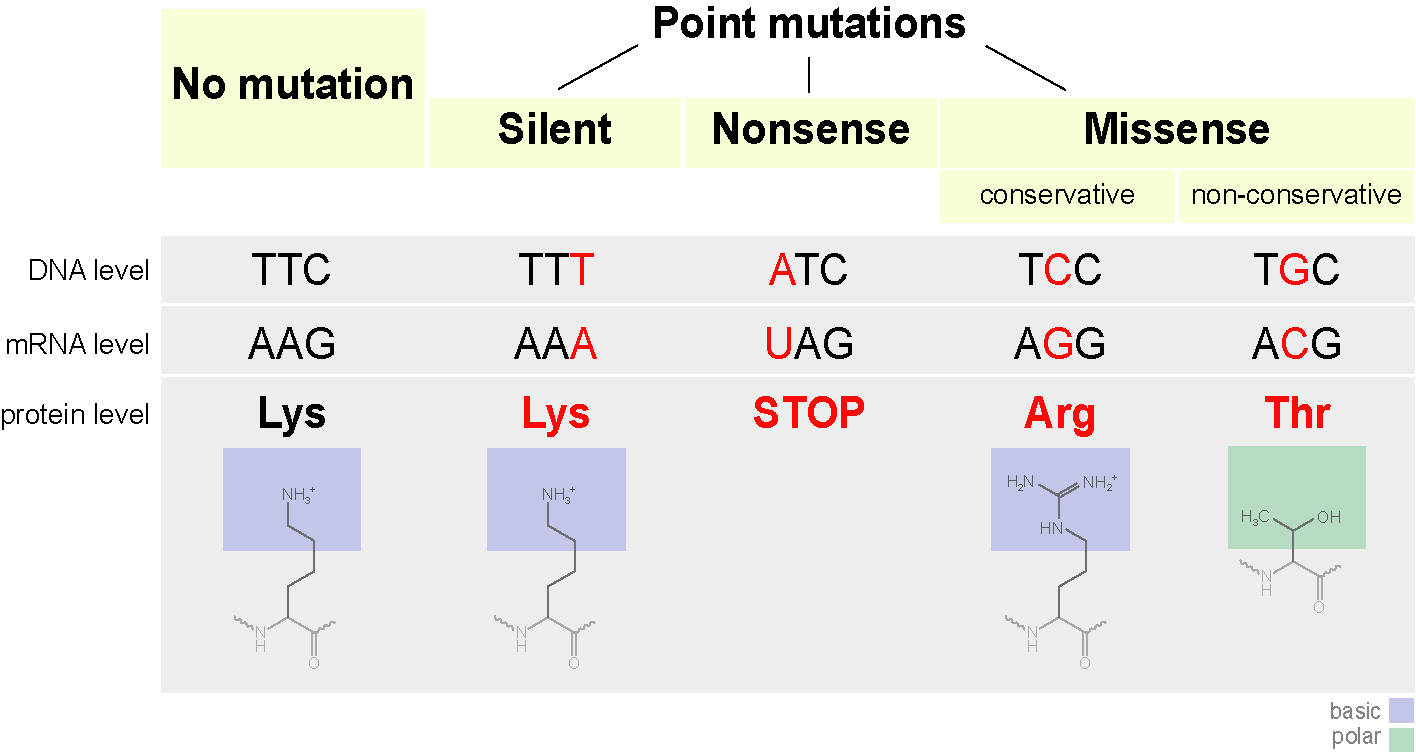
\includegraphics{ch3/Point_mutations-en.png}
\caption{Different types of substitution \index{mutation!substitution} point mutations are distinguished by their effects on the gene products; image by Jonsta247 in public domain via Wikimedia Commons.}
\end{figure}

The above processes involve copying and transferring information. As we know from experience, copying information inevitably means introducing errors. This is particularly important when passing information from parent to offspring, because then an entire organism has to develop and live based on a faulty blueprint. Changes introduced in the genome of an organism are called \index{mutation!definition} \emph{mutations}, and they can be caused either by errors in copying DNA when making a new cell (replication) or through damage to DNA through physical means (e.g.~ionizing radiation) or chemical mechanisms (e.g.~exogenous molecules that react with DNA). The simplest mutation involve a single nucleotide and are called \index{mutation!point} \emph{point mutations}. A nucleotide may be deleted, an extra nucleotide inserted, or a new one substituted instead: the three different types of substitution mutations are shown in figure \ref{fig:ch3_mutation}. Large-scale mutations may involve whole chunks of the genome that are cut out and pasted in a different location, or copied and inserted in another position, but they are typically much more rare than point mutations.

Mutations can have different effects on the mutant organism, although acquisition of super-powers has not been observed. Usually, point mutations have either little observable effect or a negative effect on the health of the mutant. A classic example is \index{sickle-cell disease} \emph{sickle-cell disease}, in which the molecules of the protein hemoglobin, responsible for carrying oxygen in the blood from the lungs to the tissues, tends to stick together and clump, resulting in sickle-shaped red blood cells. The disease is caused by a single substitution mutation in the gene that codes for one of the two components of hemoglobin, called \(\beta\)-globin. The substitution of a single nucleotide in the DNA sequence changes one amino acid in the protein from glutamate to valine, which causes the proteins to aggregate. This \index{mutation!missense} \emph{missense}\}* mutation (see figure \ref{fig:ch3_mutation}) is carried by a fraction of the human population, and those who inherit the allele \emph{allele} from both parents develop the painful and sometimes deadly disease. Such mutations that are present in some but not all of a population are called \index{mutation!polymorphism} \emph{polymorphisms}, to distinguish them from mutations that occurred in evolutionary lineages and differentiate species from each other.

One of the central questions of evolutionary biology is how frequently do mutations occur? Since mutations are generally undesirable, most living things have developed ways to minimize the frequency of errors in copying DNA, and to repair DNA damage. But although mutations are rare, they occur spontaneously in all organisms because molecular processes such as copying a DNA molecule are subject to random noise arising from thermal motion. So mutations are fundamentally a random process and we need to use \index{statistics!descriptive} \emph{descriptive statistics} to analyze data with inherent randomness.

\hypertarget{describing-data-sets-1}{%
\section{Describing data sets}\label{describing-data-sets-1}}

\label{sec:math3}

\hypertarget{central-value-of-a-data-set}{%
\subsection{central value of a data set}\label{central-value-of-a-data-set}}

A data set is a collection of measurements. These measurements can come from many kinds of sources, and can represent all sorts of quantities. One big distinction is between numerical and categorical data sets. \emph{Numerical} \index{data!numerical} data sets contain numbers, either integers or real numbers. Some examples: number of individuals in a population, length, blood pressure, concentration. \emph{Categorical} \index{data!categorical} data sets may contain numbers, symbols, or words, limited to a discrete, usually small, number of values. The word categorical is used because this kind of data corresponds to categories or states of the subject of the experiment. Some examples: genomic classification of an individual on the basis of one locus (e.g.~wild type or mutant), the state of an ion channel (open or closed), the stage of a cell in the cell cycle.

A data set contains more than one measurement, the number of them is called the size of the data set and is usually denoted by the letter \(n\). To describe a data set numerically, one can use numbers called \emph{statistics} (not to be confused with the branch of science of the same name). The most common statistics aim to describe the central value of the data set to represent a typical measurement. If you order all of the measurements from highest to lowest and then take the the middle value, you have found the \index{median} \emph{median} (if there is an even number of values, take the average between the middle two). Precisely half of the data values are less than the median and the other half are greater, so it represents the true ``middle'\,' value of the measurement. Note that the median can be calculated either for numerical or categorical data, as long as the categories can be ordered in some fashion.

The value that occurs most frequently in the data set is called its \index{mode}\emph{mode}. For some data sets, particularly those which are symmetric, the mode coincides with the mean (see next paragraph) and the median, but for many others it is distinct. The mode is the most visual of the three statistics, as it can be picked out from the histogram plot of a data set (which is described in subsection 3.2.3) as the value corresponding to the maximum frequency. The mode can also be used for both categorical and numerical data.

The average or \index{mean!data}\index{data!mean} \emph{mean} of a data set is the sum of all the values divided by the number of values. It is also called the \emph{expected value} (particularly in the context of probability, which we will discuss later) because it allows to simply predict the sum of a large number of measurements with a given mean, by multiplying the mean by the number. The mean can be calculated only for a numerical data set, since we cannot add non-numerical values.

\begin{definition}
\protect\hypertarget{def:def-mean}{}{\label{def:def-mean} }The \emph{mean} of a data set \(X\), also known as the average or the arithmetic mean is usually indicated with a bar over the variable symbol, and defined as the sum of the values divided by the number of values:
\end{definition}
\begin{equation}
  \bar X  = \frac{1}{n} \sum_{i=1}^n x_i 
\label{eq:ch3_mean_def}
\end{equation}

The mean, unlike the median, is not the middle value of the data set, instead it represents the \emph{center of mass} of the measured values \citep{whitlock_analysis_2008}. Another way of thinking of the mean is as a \textbf{weighted sum of the values in the data set}. The weights represent the frequency of occurrence of each numeric value in the data set, which we will further discuss in subsection 3.2.3.

The mean is the most frequently used statistic, but it is not always interpreted correctly. Very commonly the mean is reported as the most representative value of a data set, but that is often misleading. Here are at least two situations in which the mean can be tricky: 1) data sets with a small number of discrete values; 2) data sets with outliers, or isolated numbers very far from the mean.

\textbf{Examples of misleading means.} Mean quantities for data sets with a few quantities are not the typical value, such as in the number of children born in a year per individual, also known as the birth rate. The birth rate per year in 2013 for both the United States and Russia is 1.3\% per person, but you will have to look for a long time to find any individual who gave birth to 1.3\% of a child. While this point may be obvious, it is often overlooked when interpreting mean values.

Outliers are another source of trouble for means. For example, a single individual (let's call him or her B.G.) with a wealth of \$50 billion moves into a town of 1000 households with average wealth of \$100,000. Although none of the original residents' assets have changed, the mean wealth of the town improves dramatically, as you can calculate in one of the exercises at the end of the chapter. One can site the improved per capita (per individual) in the town as evidence of economic growth, but that is obviously misleading. In cases with such dramatic outliers, the median is more informative as representation of a typical value of the data set.

\hypertarget{exercises-6}{%
\subsection{Exercises}\label{exercises-6}}

For the (small) data sets given below, calculate the mean and the median (by hand or using a calculator) and compare the two measures of the center.

\begin{enumerate}
\def\labelenumi{\arabic{enumi}.}
\item
  Data set of the population of the city of Chicago (in millions) in the last 4 census years (2010, 2000, 1990, 1980): \{2.7, 2.9, 2.8, 3.0\}.
\item
  Data set of the numbers of the fish blacknose dace (\emph{Rhinichthys atratulus}) collected in 6 different streams in the Rock Creek watershed in Maryland: \{76, 102, 12, 55, 93, 98\}.
\item
  Data set of tuberculosis incidence rates (per 100,000 people) in the 5 largest metropolitan areas in the US in 2012: \{5.2, 6.6, 3.2, 5.5, 4.5\}.
\item
  Data set of ages of mothers at birth for five individuals: \{19, 20, 22, 32, 39\}.
\item
  Data set of ages of fathers at birth for five individuals: \{22, 23, 25, 36, 40\}.
\item
  Data set of the number of new mutations found on maternal chromosomes for five individuals: \{9, 10, 11, 26, 15\}.
\item
  Data set of the number of new mutations found on paternal chromosomes for five individuals: \{39, 43, 51, 53, 91\}.
\item
  Consider the hypothetical town with 1000 households with mean and median wealth of \$100,000 and one person with assets for \$50 billion. Calculate the mean value of the combined data set, and compare it to the new median value.
\item
  Suppose you'd like to add a new observation to a data set; e.g.~the 6-th largest metropolitan area (Philadelphia) to the tuberculosis incidence data set, which is 3.0. Calculate the mean of the 6-values data set, without using the 5 values in the original data set, but only using the mean of the 5-value data set and the new value. Generalize this to calculating the sample mean for any \(n\)-value data set, given the mean of the \(n-1\) values, plus one new value.
\end{enumerate}

\hypertarget{spread-of-a-data-set}{%
\subsection{spread of a data set}\label{spread-of-a-data-set}}

The center of a data set is obviously important, but so is the spread around the center. Sometimes the spread is caused by noise or error, for example in a data set of repeated measurements of the same variable under the same conditions. Other times the variance is due to real changes in the system, or due to inherent randomness of the system, and the size of the spread, as well as the shape of the histogram are important for understanding the mechanism. The simplest way to describe the spread of a numerical data set is to look at the difference between the maximum and minimum values, called the \index{data!range} \emph{range}. However, it is obviously influenced by outliers, since the extreme values are used. To describe the typical spread, we need to use all the values in the data set, and see how far each one is from the center, measured by the mean.

There is a problem with the naive approach: if we just add up all the differences of data values from the mean, the positives will cancel the negatives, and we'll get an artificially low spread. One way to correct this is to take the absolute value of the differences before adding them up. However, for somewhat deep mathematical reasons, the standard measure of spread uses not absolute values, but squares of the differences, and then divides that sum not by the number of data points \(n\) but by \(n-1\).

\begin{definition}
\protect\hypertarget{def:def-var}{}{\label{def:def-var} }The \emph{variance} of a data set \(X\) with \(n\) values is the sum of the squared differences of each value of the variable from the mean, divided by \(n-1\):
\end{definition}
\begin{equation}
 Var(X) = \frac{1}{n-1} \sum_{i=1}^n (\bar X - x_i)^2
\end{equation}

The variance is a sum of square differences, so its dimension is the square of the dimensions of the measurements in \(X\). In order to obtain a measure of the spread comparable to the values of \(X\), we take the square root of variance and call it the \index{data!standard deviation} \emph{standard deviation} of the data set \(X\):
\begin{equation}
\sigma(X) = \sqrt{\frac{1}{n-1} \sum_{i=1}^n (\bar X - x_i)^2}
\end{equation}

Just as the mean is a weighted average of all of the values in the data set, the variance is a weighted average of all the squared deviations of the data from the mean.

\hypertarget{exercises-7}{%
\subsection{Exercises:}\label{exercises-7}}

For the (small) data sets below, calculate the range, variance, and standard deviation (by hand or using a calculator). Compare the range and the standard deviation for each case: which one is larger? by how much?

\begin{enumerate}
\def\labelenumi{\arabic{enumi}.}
\item
  Data set of the population of the city of Chicago (in millions) in the last 4 census years (2010, 2000, 1990, 1980): \{2.7, 2.9, 2.8, 3.0\}.
\item
  Data set of the numbers of the fish blacknose dace (\emph{Rhinichthys atratulus}) collected in 6 different streams in the Rock Creek watershed in Maryland: \{76, 102, 12, 55, 93, 98\}.
\item
  Data set of tuberculosis incidence rates (per 100,000 people) in the 5 largest metropolitan areas in the US in 2012: \{5.2, 6.6, 3.2, 5.5, 4.5\}.
\item
  Data set of ages of mothers at birth for five individuals: \{19, 20, 22, 32, 39\}.
\item
  Data set of ages of fathers at birth for five individuals: \{22, 23, 25, 36, 40\}.
\item
  Data set of the number of new mutations found on maternal chromosomes for five individuals: \{9, 10, 11, 26, 15\}.
\item
  Data set of the number of new mutations found on paternal chromosomes for five individuals: \{39, 43, 51, 53, 91\}.
\item
  Consider the hypothetical town with 1000 households with mean and median wealth of \$100,000 and one person with assets for \$50 billion. Calculate the mean value of the combined data set, and compare it to the new median value.
\item
  (harder) Suppose that a data set has a fixed range (e.g.~all values have to lie between 0 and 1). What is the greatest possible standard deviation for any data set within the range? Hint: think about how to place the points as far from the mean as possible. How do the data sets above relate to your prediction?\}
\end{enumerate}

\hypertarget{describing-data-sets-in-graphs}{%
\subsection{describing data sets in graphs}\label{describing-data-sets-in-graphs}}

Data sets can be presented visually to indicate the frequency of different values. This can be done in a number of ways, depending on the kind of data set. For a data set with only a few values, e.g.~a categorical data set, a good way to represent it is with a pie chart. Each category is represented by a slice of the pie with the area of the same share of the pie as the fraction of the data set in the category. There is some evidence, however, that pie charts can be misleading to the eye, so R does not recommend using them.

For a numerical data set it is useful to plot the frequencies of a range of values, which is called a \index{histogram!definition} \emph{histogram}. Its independent axis has the values of the data variable, and the dependent axis has the frequency of those values. If the data set consists of real numbers that range across an interval, that interval is divided into subintervals (usually of equal size), called bins, and the number of measurements in each bin is indicated on the y-axis. In order to be visually informative, there should be a reasonable number (usually no more than a few dozen, although it varies) of bins. The most frequent measurements are represented as the highest bars or points on the histogram. Histograms can denote either the counts of measurements in each bin, or to show the fraction of the total number of measurements in each bin. The only difference between those two kinds of histogram is the scale of the y-axis, and, confusingly, both can be called frequencies.

\begin{figure}

{\centering 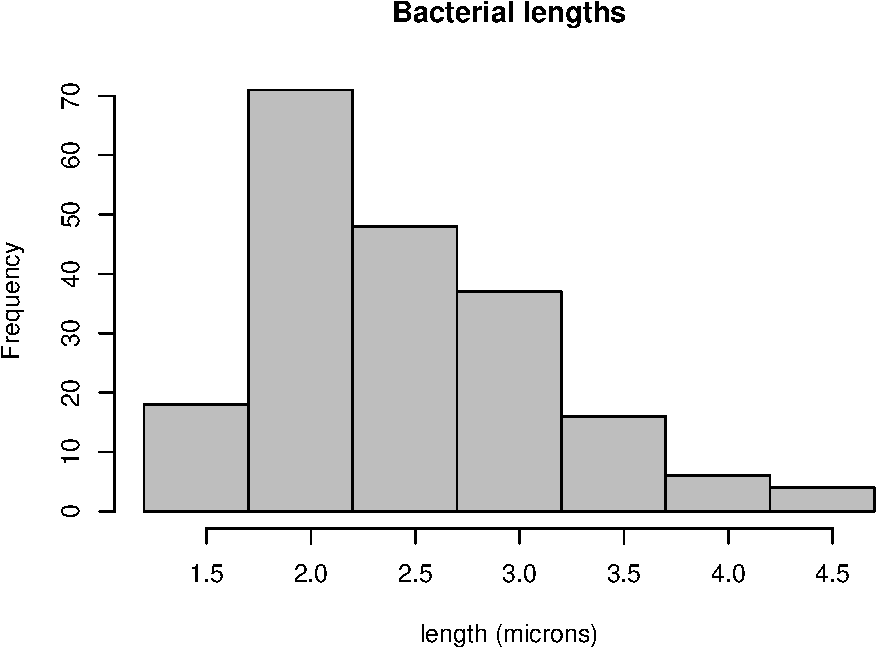
\includegraphics[width=0.5\linewidth]{QuantLife_files/figure-latex/fig-ch3-bacillus-1} 

}

\caption{Length of bacteria Bacillus subtilis measured under the microscope as discrete values with step of 0.5; data from citep{watkins-intro-stats}}\label{fig:fig-ch3-bacillus}
\end{figure}

A histogram of the measured lengths of the bacterium \emph{Bacillus subtilis} is shown in figure \ref{fig:ch3_bacillus}. The data set was measured in increments in half a micron, with numbers varying between 1.5 and 4.5 microns. The histogram shows that the most common measurement (the mode) is 2 \(\mu m\). Adding up all of the frequencies in the histogram tells us that there are approximately 200 total values in the data set. This allows us to find the median value by counting the frequencies of the first few bins until we get to 100 (the median point), which resides in the bin for 2.5 \(\mu m\). It is a little bit more difficult to estimate the mean, but it should be clear that the center of mass of the histogram is also near 2.5 (it is actually 2.49). Finally, the hardest task is estimating the spread of the data set, such as the the standard deviation, based on the histogram. The range of the data set is \(4.5-1.5 = 3\), so we know for sure that it is less than 1.5. The histogram shows that the deviations from the mean value of 2.5 range from 2 (rarely) to 0.5 (most prevalent). This should give you an idea that the weighted average of the deviations is less than 1. Indeed, the correct standard deviation is about 0.67.

There are different ways of plotting data sets that have more than one variable. For instance, a data set measured over time is called a time series. If the values are plotted with the corresponding times on the x-axis, then it is called a \index{plot!time} \emph{time plot}. This is useful to show the changes of the values of your variable over time. If the data set doesn't undergo any significant changes over time, it makes more sense to represent it as a pie chart or histogram. More generally, one may plot two variables measured together on a single plot, which is called a \index{plot!scatter} \emph{scatterplot}. We will explore such plots and the relationships between two measured variables in chapter 4.

\hypertarget{exercises-8}{%
\subsection{Exercises}\label{exercises-8}}

Answer the following questions, based on the histograms in figure \ref{fig:ch3_mut} (mutation data) and in figure \ref{fig:ch3_HR} (heart rate data).

\begin{enumerate}
\def\labelenumi{\arabic{enumi}.}
\item
  How many people in the mutation data have fathers either younger than 20 or older than 40? How many have more than 80 new mutations? \index{medical!heart rate}
\item
  Estimate the median and mean of the two variables in the mutation data set.
\item
  State the range of each data set, and estimate the standard deviation of the two variables in the mutation data set.
\item
  How many people in the heart rate data have heart rates greater than 80 bpm? How many have body temperature less that 97 F?
\item
  Estimate the median and mean of the two variables in the heart rate data set.
\item
  State the range of each data set, and estimate the standard deviation of the two variables in the heart rate data set.
\end{enumerate}

\begin{Shaded}
\begin{Highlighting}[]
\NormalTok{my\_data \textless{}{-}}\StringTok{ }\KeywordTok{read.table}\NormalTok{(}\StringTok{"data/HR\_temp.txt"}\NormalTok{, }\DataTypeTok{header =} \OtherTok{TRUE}\NormalTok{)}
\KeywordTok{hist}\NormalTok{(my\_data}\OperatorTok{$}\NormalTok{HR, }\DataTypeTok{col =} \StringTok{"gray"}\NormalTok{, }\DataTypeTok{main =} \StringTok{"Heart rate data"}\NormalTok{, }
    \DataTypeTok{xlab =} \StringTok{"heart rate (bpm)"}\NormalTok{)}
\KeywordTok{hist}\NormalTok{(my\_data}\OperatorTok{$}\NormalTok{Temp, }\DataTypeTok{col =} \StringTok{"gray"}\NormalTok{, }\DataTypeTok{main =} \StringTok{"Body temperature data"}\NormalTok{, }
    \DataTypeTok{xlab =} \StringTok{"temperature (F)"}\NormalTok{)}
\end{Highlighting}
\end{Shaded}

\begin{figure}

{\centering 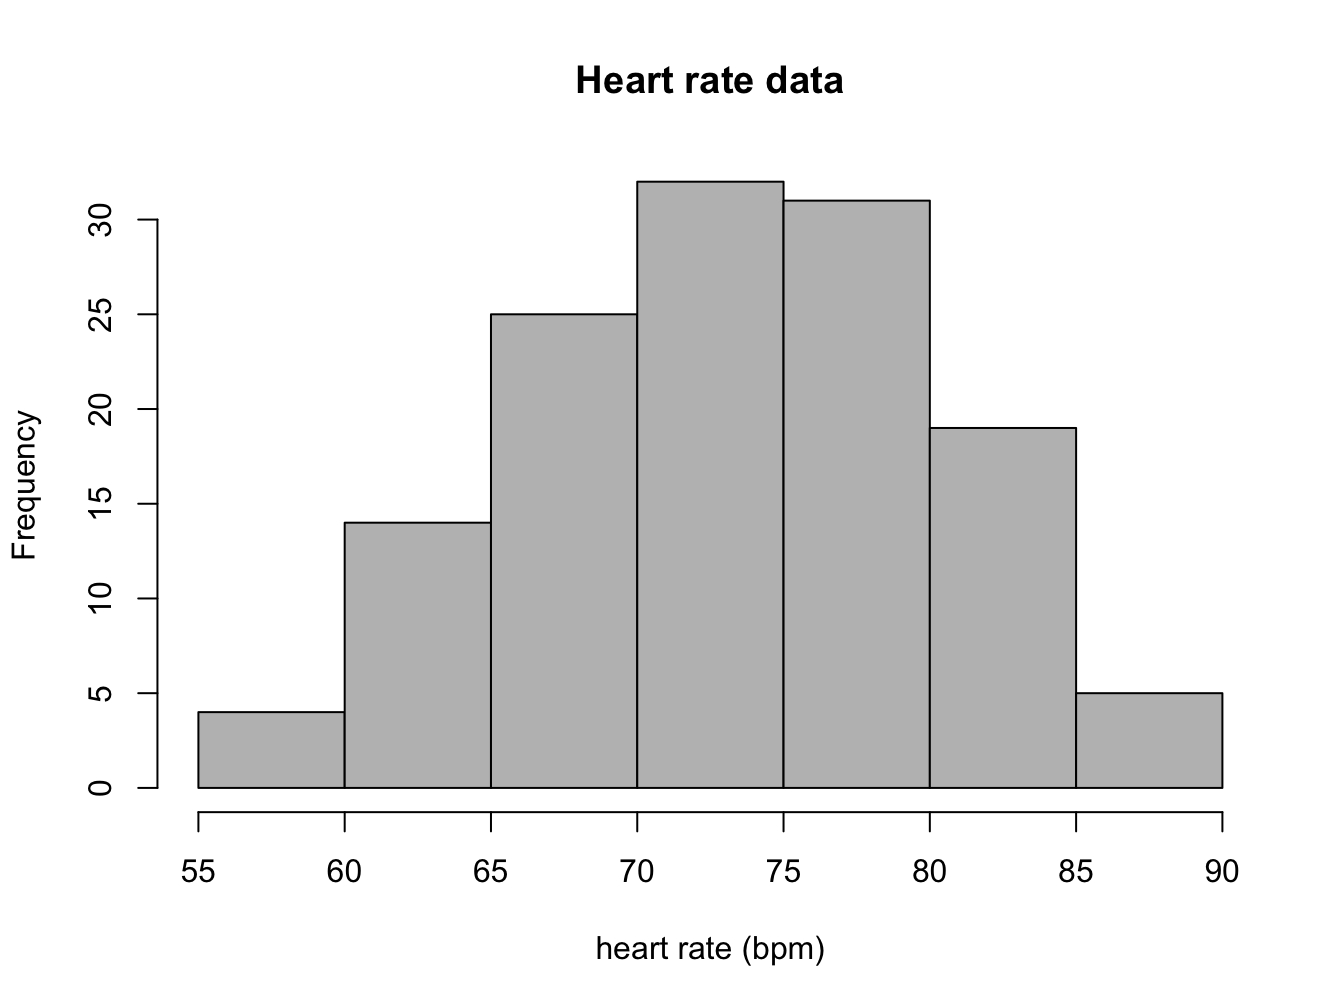
\includegraphics[width=0.5\linewidth]{QuantLife_files/figure-latex/fig-ch3-HR-1} 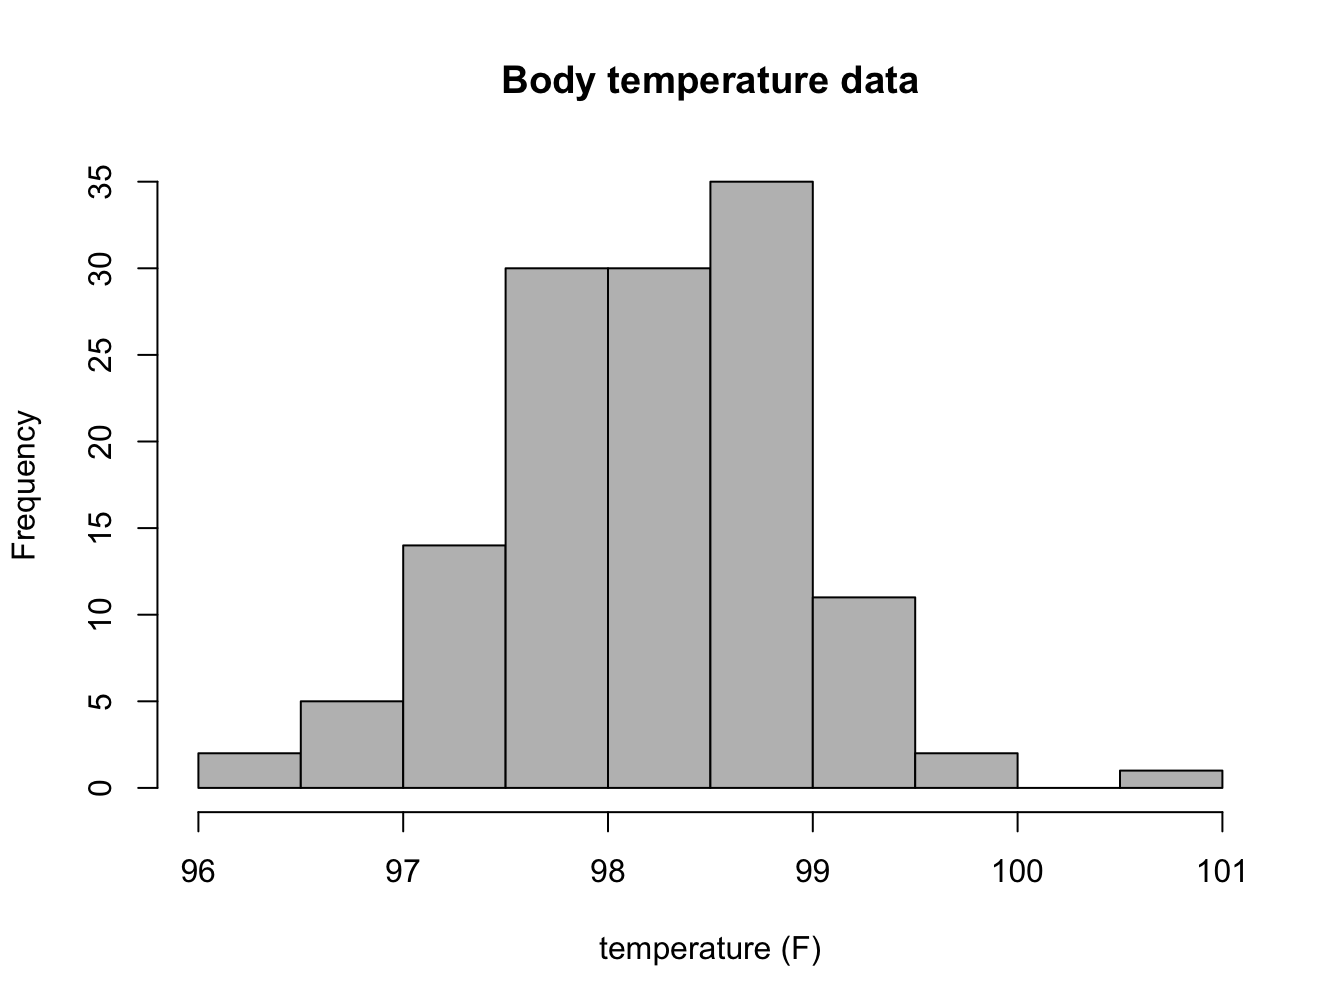
\includegraphics[width=0.5\linewidth]{QuantLife_files/figure-latex/fig-ch3-HR-2} 

}

\caption{Histograms of heart rates and body temperatures}\label{fig:fig-ch3-HR}
\end{figure}

\textbackslash begin\{figure\}

\{\centering 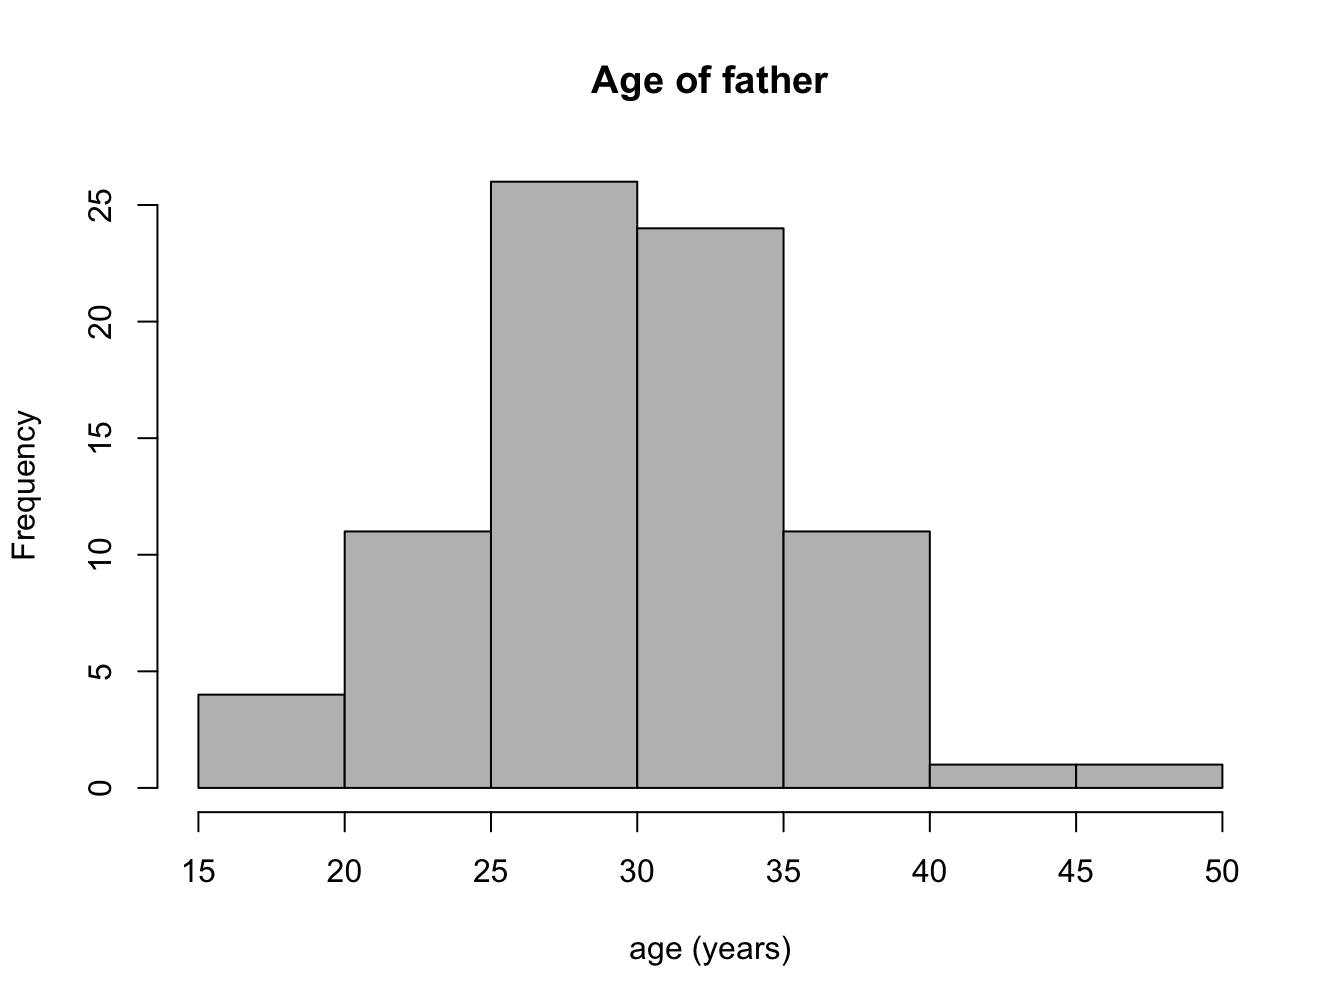
\includegraphics[width=0.5\linewidth]{QuantLife_files/figure-latex/fig-ch3-mut-1} 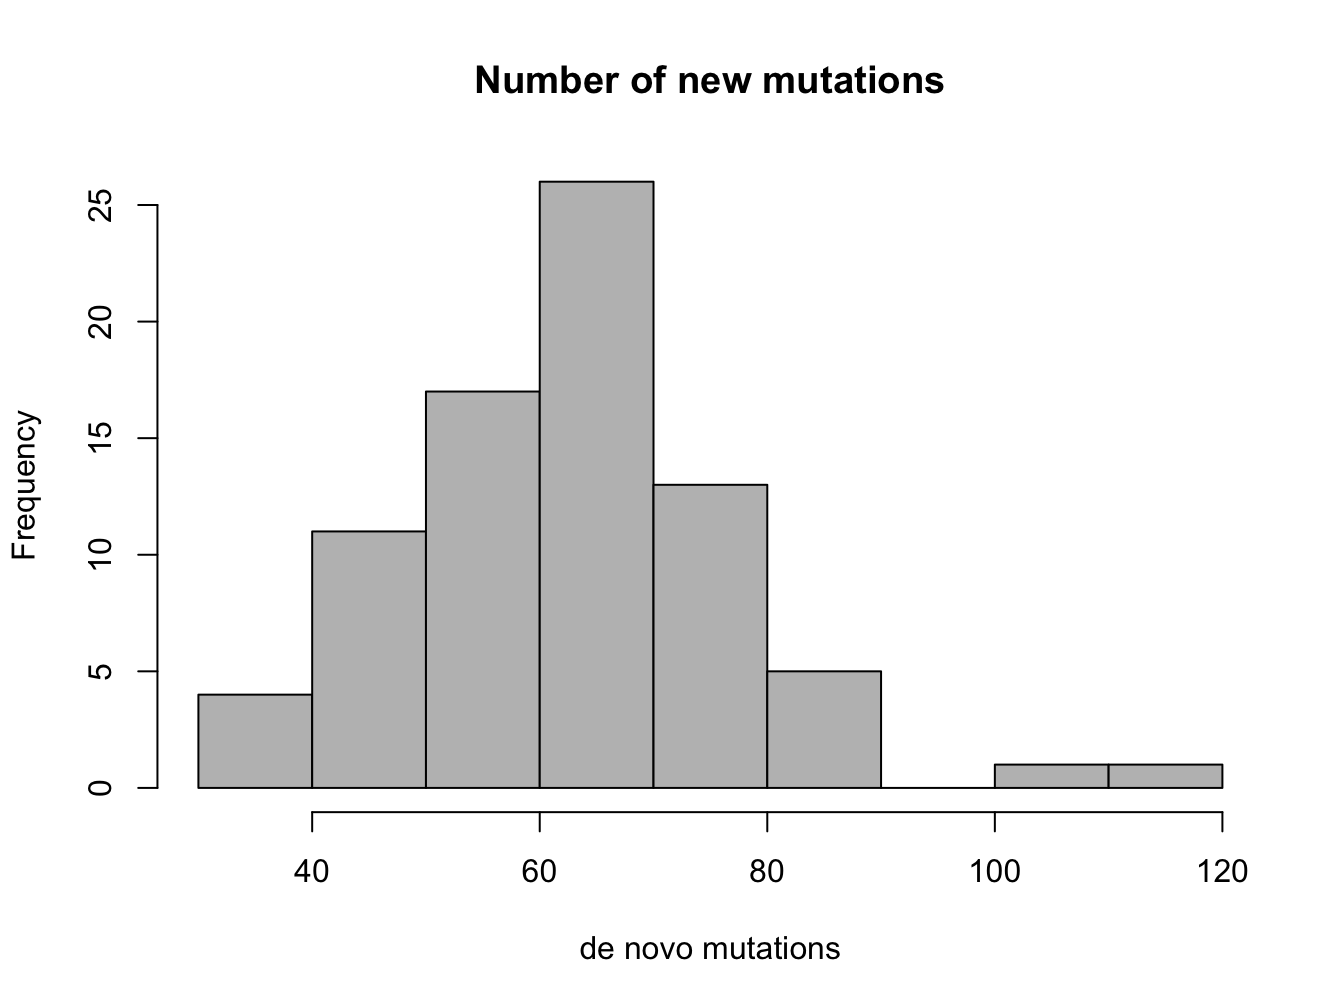
\includegraphics[width=0.5\linewidth]{QuantLife_files/figure-latex/fig-ch3-mut-2}

\}

\textbackslash caption\{Histograms of paternal ages and the number of new mutations from 73 families; data from citep\{kong\_rate\_2012\}\}\label{fig:fig-ch3-mut}
\textbackslash end\{figure\}

\hypertarget{working-with-data-in-r}{%
\section{Working with data in R}\label{working-with-data-in-r}}

\label{sec:comp3}

\hypertarget{reading-in-data-into-data-frames}{%
\subsection{reading in data into data frames}\label{reading-in-data-into-data-frames}}

One way to input data into R is to read in a text file, where several variables are stored in columns. For instance, the file \texttt{HR\_temp.txt} contains three variables: body temperature (in Fahrenheit), sex (1 for male, 2 for female), and heart rate (in beats per minute). The values for the variables are arranged in columns, while first row of the file contains the names of the variables (Temp, Sex, and HR, respectively). Note that the data file has to be saved into the same folder as the .Rmd file week1.Rmd for this to work.

\begin{Shaded}
\begin{Highlighting}[]
\NormalTok{vitals \textless{}{-}}\StringTok{ }\KeywordTok{read.table}\NormalTok{(}\DataTypeTok{file =} \StringTok{"data/HR\_temp.txt"}\NormalTok{, }\DataTypeTok{header =} \OtherTok{TRUE}\NormalTok{)}
\KeywordTok{plot}\NormalTok{(vitals}\OperatorTok{$}\NormalTok{HR, vitals}\OperatorTok{$}\NormalTok{Temp, }\DataTypeTok{main =} \StringTok{"Body temp as function of heart rate"}\NormalTok{, }
    \DataTypeTok{xlab =} \StringTok{"heart rate (bpm)"}\NormalTok{, }\DataTypeTok{ylab =} \StringTok{"body temperature (F)"}\NormalTok{)}
\NormalTok{mTemp \textless{}{-}}\StringTok{ }\KeywordTok{mean}\NormalTok{(vitals}\OperatorTok{$}\NormalTok{Temp)}
\NormalTok{sdTemp \textless{}{-}}\StringTok{ }\KeywordTok{sd}\NormalTok{(vitals}\OperatorTok{$}\NormalTok{Temp)}
\KeywordTok{abline}\NormalTok{(mTemp, }\DecValTok{0}\NormalTok{)}
\end{Highlighting}
\end{Shaded}

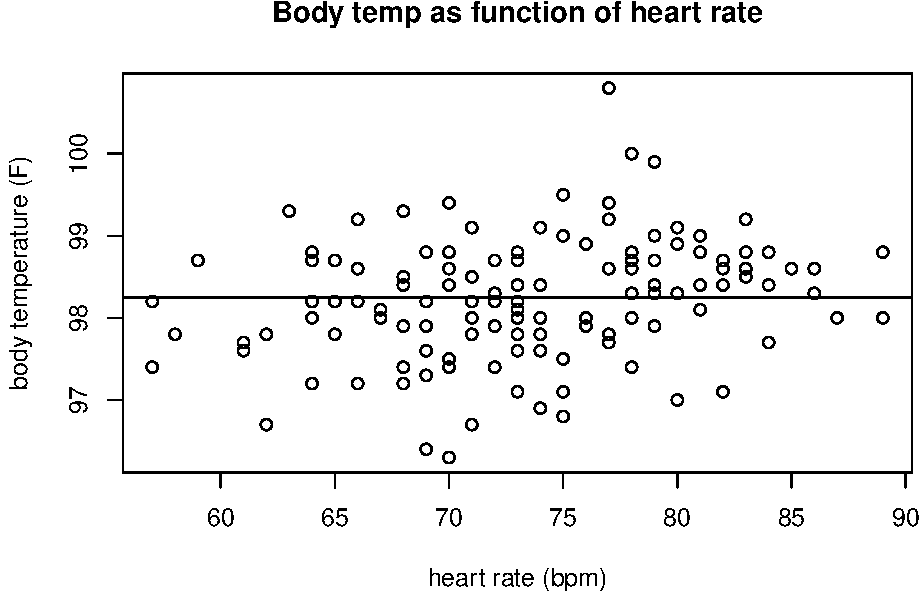
\includegraphics{QuantLife_files/figure-latex/unnamed-chunk-58-1.pdf}

\begin{Shaded}
\begin{Highlighting}[]
\KeywordTok{mean}\NormalTok{(vitals}\OperatorTok{$}\NormalTok{HR)}
\end{Highlighting}
\end{Shaded}

\begin{verbatim}
## [1] 73.76154
\end{verbatim}

\begin{Shaded}
\begin{Highlighting}[]
\KeywordTok{sd}\NormalTok{(vitals}\OperatorTok{$}\NormalTok{HR)}
\end{Highlighting}
\end{Shaded}

\begin{verbatim}
## [1] 7.062077
\end{verbatim}

The R command read.table() reads this file and and puts it into a \emph{data frame} called data. The three variables are stored inside the data frame, and can be accessed by appending the dollar sign and variable name to the data frame, so \texttt{data\$HR} refers to only the heart rates, and \texttt{data\$Temp} refers to the body temperatures. The plot shows the relationship of the two data variables, and the function \texttt{abline(98.6,0)} plots a line with the intercept 98.6a and slope 0 on top of the scatterplot.

You can also load data from a package, e.g.~\texttt{HistData}, which contains many classic data sets. Got to the Packages tab in the lower right window in R Studio, click Install and type \texttt{HistData}. We will use the data set called \texttt{Galton} that contains the heights of parents (the mean of mother's and father's) and their children, in variables parent and child. The script below plots the two variables, with parent as the independent (explanatory) variable and child as the dependent (response) variable.

\begin{Shaded}
\begin{Highlighting}[]
\KeywordTok{library}\NormalTok{(HistData)}
\KeywordTok{plot}\NormalTok{(Galton}\OperatorTok{$}\NormalTok{parent, Galton}\OperatorTok{$}\NormalTok{child, }\DataTypeTok{main =} \StringTok{"Height of child vs average height of parents"}\NormalTok{, }
    \DataTypeTok{xlab =} \StringTok{"parent height (inches)"}\NormalTok{, }\DataTypeTok{ylab =} \StringTok{"child height (inches)"}\NormalTok{)}
\end{Highlighting}
\end{Shaded}

\begin{center}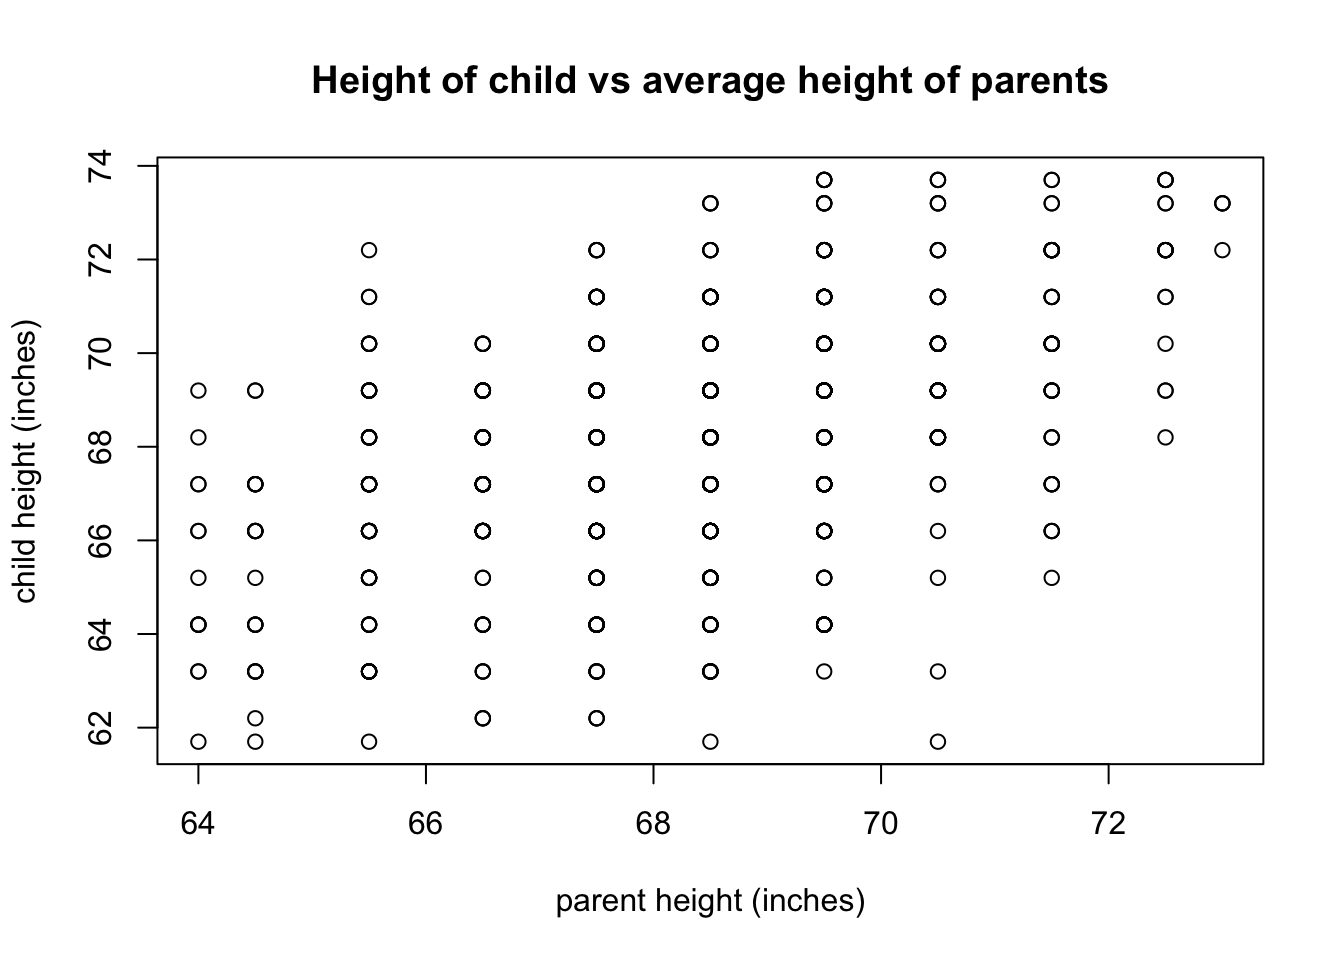
\includegraphics{QuantLife_files/figure-latex/unnamed-chunk-59-1} \end{center}

\begin{Shaded}
\begin{Highlighting}[]
\KeywordTok{summary}\NormalTok{(Galton}\OperatorTok{$}\NormalTok{parent)}
\end{Highlighting}
\end{Shaded}

\begin{verbatim}
##    Min. 1st Qu.  Median    Mean 3rd Qu.    Max. 
##   64.00   67.50   68.50   68.31   69.50   73.00
\end{verbatim}

\begin{Shaded}
\begin{Highlighting}[]
\KeywordTok{summary}\NormalTok{(Galton}\OperatorTok{$}\NormalTok{child)}
\end{Highlighting}
\end{Shaded}

\begin{verbatim}
##    Min. 1st Qu.  Median    Mean 3rd Qu.    Max. 
##   61.70   66.20   68.20   68.09   70.20   73.70
\end{verbatim}

\hypertarget{descriptive-statistics}{%
\subsection{descriptive statistics}\label{descriptive-statistics}}

One can also calculate basic descriptive statistics as follows:

\begin{Shaded}
\begin{Highlighting}[]
\KeywordTok{paste}\NormalTok{(}\StringTok{"The mean parental height is:"}\NormalTok{, }\KeywordTok{mean}\NormalTok{(Galton}\OperatorTok{$}\NormalTok{parent))}
\end{Highlighting}
\end{Shaded}

\begin{verbatim}
## [1] "The mean parental height is: 68.3081896551724"
\end{verbatim}

\begin{Shaded}
\begin{Highlighting}[]
\KeywordTok{paste}\NormalTok{(}\StringTok{"The mean child height is:"}\NormalTok{, }\KeywordTok{mean}\NormalTok{(Galton}\OperatorTok{$}\NormalTok{child))}
\end{Highlighting}
\end{Shaded}

\begin{verbatim}
## [1] "The mean child height is: 68.0884698275862"
\end{verbatim}

\begin{Shaded}
\begin{Highlighting}[]
\KeywordTok{paste}\NormalTok{(}\StringTok{"The standard deviation of parental height is:"}\NormalTok{, }\KeywordTok{sd}\NormalTok{(Galton}\OperatorTok{$}\NormalTok{parent))}
\end{Highlighting}
\end{Shaded}

\begin{verbatim}
## [1] "The standard deviation of parental height is: 1.78733340172202"
\end{verbatim}

\begin{Shaded}
\begin{Highlighting}[]
\KeywordTok{paste}\NormalTok{(}\StringTok{"The standard deviation of  child height is:"}\NormalTok{, }\KeywordTok{sd}\NormalTok{(Galton}\OperatorTok{$}\NormalTok{child))}
\end{Highlighting}
\end{Shaded}

\begin{verbatim}
## [1] "The standard deviation of  child height is: 2.51794136627677"
\end{verbatim}

Why do you think the standard deviation of parental height is much smaller?

R has histogram function \texttt{hist()}, which does a passable job of representing the distribution of a variable such as child height or parent height. Compare the width of the two distributions and consider why they are different.

\begin{Shaded}
\begin{Highlighting}[]
\KeywordTok{hist}\NormalTok{(Galton}\OperatorTok{$}\NormalTok{child)}
\KeywordTok{hist}\NormalTok{(Galton}\OperatorTok{$}\NormalTok{parent)}
\end{Highlighting}
\end{Shaded}

\begin{center}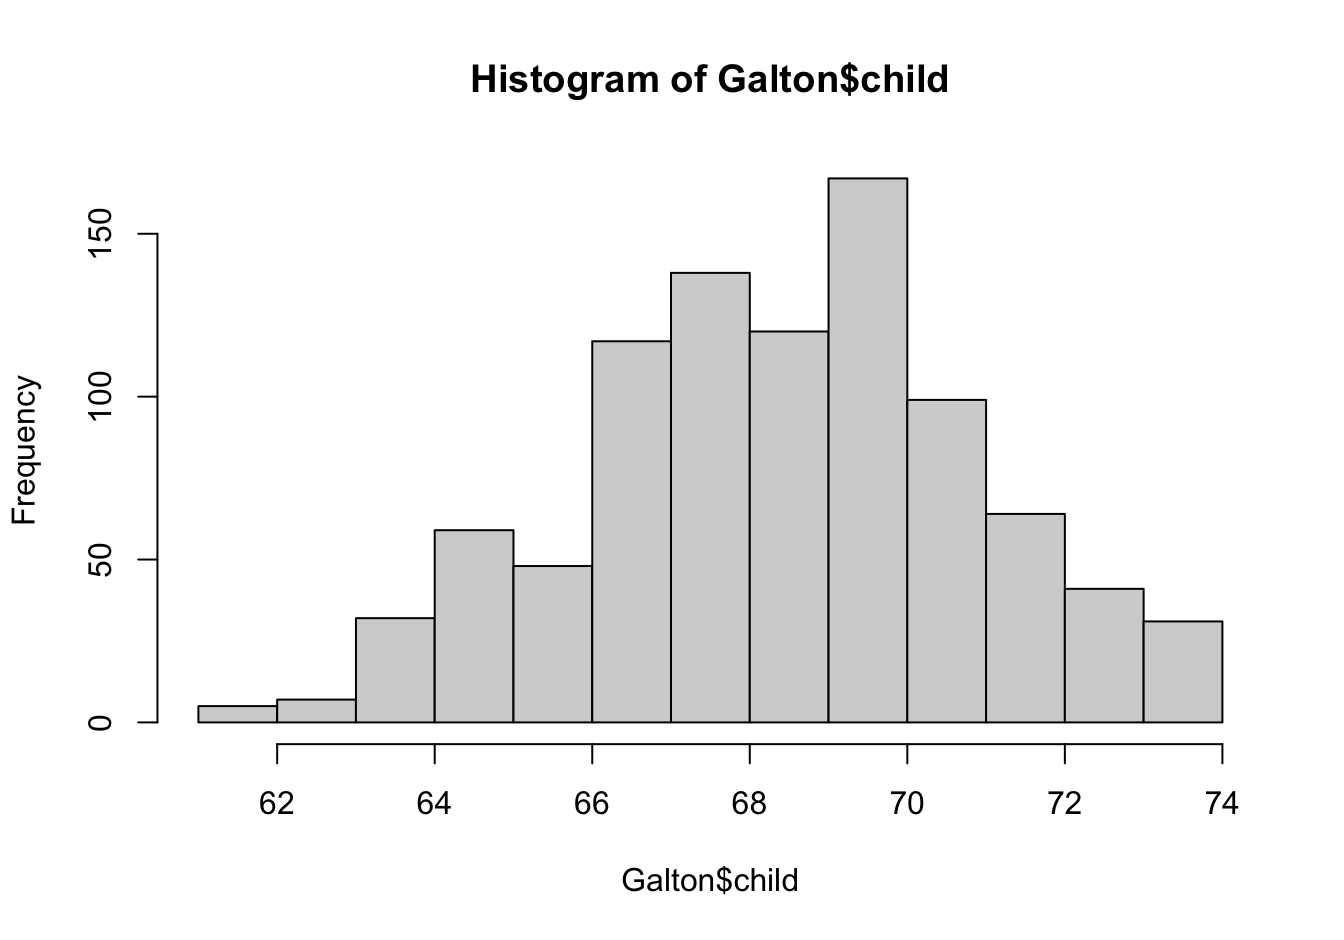
\includegraphics[width=0.5\linewidth]{QuantLife_files/figure-latex/unnamed-chunk-61-1} 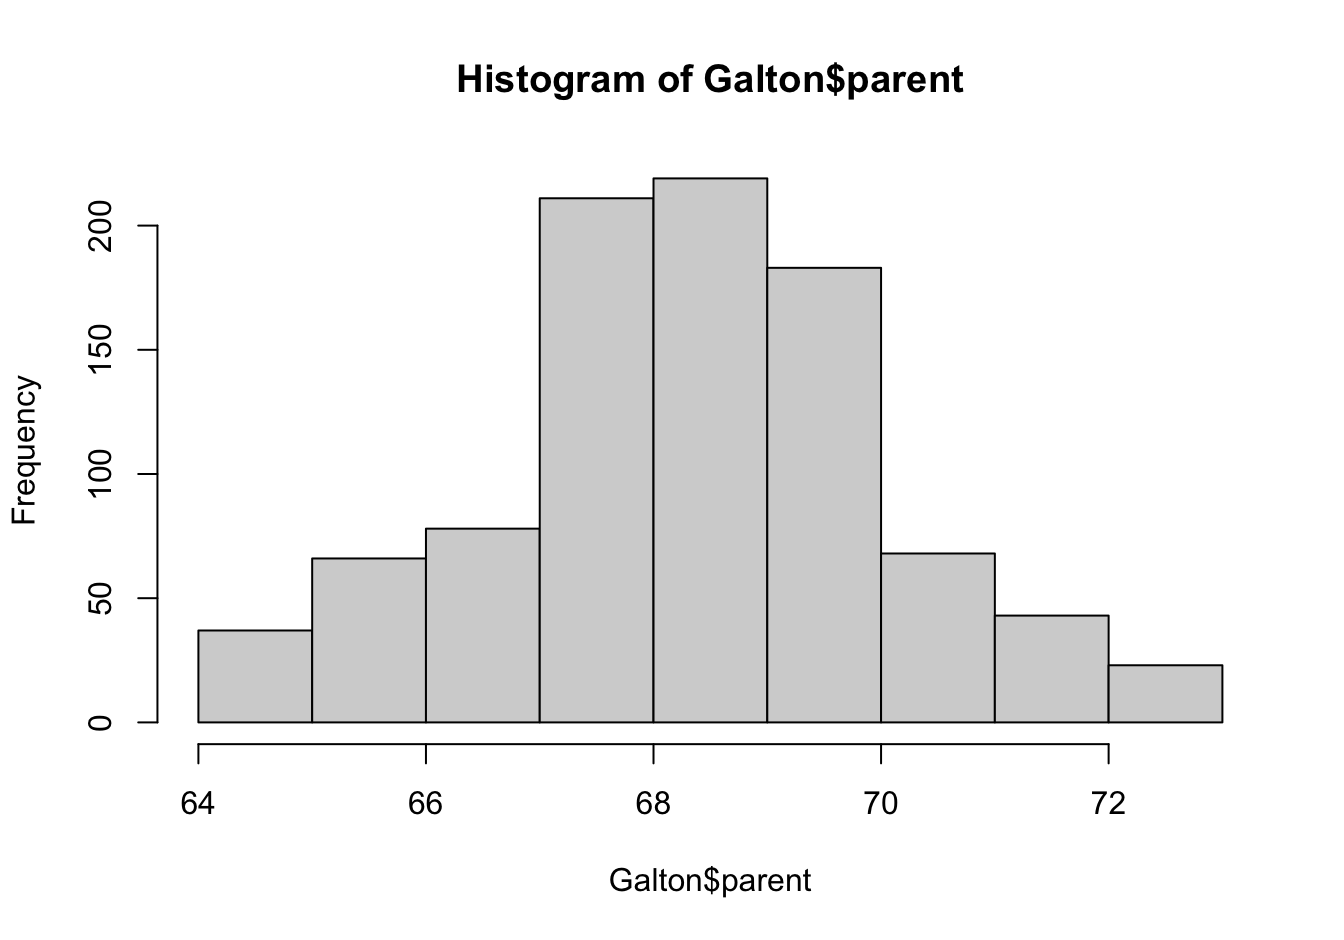
\includegraphics[width=0.5\linewidth]{QuantLife_files/figure-latex/unnamed-chunk-61-2} \end{center}

\hypertarget{exercises-9}{%
\subsection{Exercises:}\label{exercises-9}}

The following code chunks contain errors. Find and fix them so they work as intended.

\begin{enumerate}
\def\labelenumi{\arabic{enumi}.}
\tightlist
\item
  Calculate the mean and standard deviation of the heart rates of the first 30 individuals in the data frame vitals:
\end{enumerate}

\begin{Shaded}
\begin{Highlighting}[]
\KeywordTok{mean}\NormalTok{(vitals}\OperatorTok{$}\NormalTok{HR[}\DecValTok{30}\NormalTok{])}
\end{Highlighting}
\end{Shaded}

\begin{verbatim}
## [1] 64
\end{verbatim}

\begin{Shaded}
\begin{Highlighting}[]
\KeywordTok{sd}\NormalTok{(vitals}\OperatorTok{$}\NormalTok{HR[}\DecValTok{30}\NormalTok{])}
\end{Highlighting}
\end{Shaded}

\begin{verbatim}
## [1] NA
\end{verbatim}

\begin{enumerate}
\def\labelenumi{\arabic{enumi}.}
\setcounter{enumi}{1}
\tightlist
\item
  Calculate the mean and standard deviation of the ratio of heart rates to body temperatures for the data set vitals:
\end{enumerate}

\begin{Shaded}
\begin{Highlighting}[]
\KeywordTok{mean}\NormalTok{(vitals}\OperatorTok{$}\NormalTok{HR}\OperatorTok{/}\NormalTok{Temp)}
\KeywordTok{sd}\NormalTok{(vitals}\OperatorTok{$}\NormalTok{HR}\OperatorTok{/}\NormalTok{Temp)}
\end{Highlighting}
\end{Shaded}

\begin{enumerate}
\def\labelenumi{\arabic{enumi}.}
\setcounter{enumi}{2}
\tightlist
\item
  Plot a scatterplot of the child heights as the response variable and the parent heights and the explanatory variable, and overlay the line y=x on top.
\end{enumerate}

\begin{Shaded}
\begin{Highlighting}[]
\KeywordTok{plot}\NormalTok{(parent, child, }\DataTypeTok{main =} \StringTok{\textquotesingle{}Height of child vs average height of parents\textquotesingle{}}\NormalTok{, }\DataTypeTok{xlab=} \StringTok{\textquotesingle{}child height (inches)\textquotesingle{}}\NormalTok{, }\DataTypeTok{ylab=} \StringTok{\textquotesingle{}parent height (inches)\textquotesingle{}}\NormalTok{)}
\KeywordTok{abline}\NormalTok{(}\DecValTok{1}\NormalTok{,}\DecValTok{0}\NormalTok{)}
\end{Highlighting}
\end{Shaded}

\begin{enumerate}
\def\labelenumi{\arabic{enumi}.}
\setcounter{enumi}{3}
\tightlist
\item
  Calculate the median of both parent and child heights:
\end{enumerate}

\begin{Shaded}
\begin{Highlighting}[]
\KeywordTok{median}\NormalTok{(Galton)}
\end{Highlighting}
\end{Shaded}

\begin{enumerate}
\def\labelenumi{\arabic{enumi}.}
\setcounter{enumi}{4}
\tightlist
\item
  Plot the histogram of parent heights of the first half of the group:
\end{enumerate}

\begin{Shaded}
\begin{Highlighting}[]
\KeywordTok{hist}\NormalTok{(Galton}\OperatorTok{$}\NormalTok{parent}\OperatorTok{/}\DecValTok{2}\NormalTok{)}
\end{Highlighting}
\end{Shaded}

\begin{enumerate}
\def\labelenumi{\arabic{enumi}.}
\setcounter{enumi}{5}
\tightlist
\item
  Plot the histogram for the ratio of parent and child heights for the entire data set and calculate its mean and variance:
\end{enumerate}

\begin{Shaded}
\begin{Highlighting}[]
\KeywordTok{hist}\NormalTok{(Galton}\OperatorTok{$}\NormalTok{parent}\OperatorTok{/}\NormalTok{child)}
\KeywordTok{mean}\NormalTok{(Galton}\OperatorTok{$}\NormalTok{parent}\OperatorTok{/}\NormalTok{child)}
\KeywordTok{sd}\NormalTok{(Galton}\OperatorTok{$}\NormalTok{parent}\OperatorTok{/}\NormalTok{child)}
\end{Highlighting}
\end{Shaded}

\hypertarget{r-assignment-2}{%
\section{R Assignment}\label{r-assignment-2}}

In this section you will read in three different data files and assign each data frame a descriptive name, e.g.~Alcohol, and then plot and fit relationship between the variables within each data frame. Your task will be to choose the parameters slope and intercept that produce a plot that does a decent job of resembling the data, meaning that the line should pass through the scatterplot and capture its trend (rising or falling) fairly well.

\begin{enumerate}
\def\labelenumi{\arabic{enumi}.}
\tightlist
\item
  Read in the mutations data set found in the file \texttt{kong\_mutation\_data.txt}, using the option \texttt{header=TRUE}. It contains three variables: \texttt{PatAge} (paternal age in years), \texttt{MatAge} (maternal age in years), and \texttt{Mutations} (number of de novo mutations).
\end{enumerate}

\begin{enumerate}
\def\labelenumi{\alph{enumi})}
\item
  Print the mean and standard deviation of each variable, and generate histograms of all three variables.
\item
  Plot \texttt{Mutations} as a function \texttt{PatAge} using circles (the default type). Assign values to slope and intercept variables, calculate a vector of predicted values for \texttt{Mutation}, and use \texttt{lines()} to add a plot of the predicted values to the data plot. Try different values of the slope and intercept until you find ones that fit the data reasonably well. Calculate the sum (use the \texttt{sum()} function) of squared differences between the vector \texttt{Mutation} and the vector of predicted values and print it out.
\end{enumerate}

\begin{Shaded}
\begin{Highlighting}[]
\CommentTok{\# THIS IS A COMMENT. YOUR CODE GOES HERE }
\end{Highlighting}
\end{Shaded}

\begin{enumerate}
\def\labelenumi{\alph{enumi})}
\setcounter{enumi}{2}
\tightlist
\item
  Make a plot of \texttt{Mutations} vs \texttt{MatAge} using circles (the default type). Assign values to slope and intercept variables, calculate a vector of predicted values for \texttt{Mutation}, and use \texttt{lines()} to add a plot of the predicted values to the data plot. Try different values of the slope and intercept until you find ones that fit the data reasonably well. Calculate the sum (use the \texttt{sum()} function) of squared differences between the vector \texttt{Mutation} and the vector of predicted values and print it out.
\end{enumerate}

\begin{Shaded}
\begin{Highlighting}[]
\CommentTok{\# THIS IS A COMMENT. YOUR CODE GOES HERE }
\end{Highlighting}
\end{Shaded}

\begin{enumerate}
\def\labelenumi{\arabic{enumi}.}
\setcounter{enumi}{1}
\tightlist
\item
  Read in the data set of heart rates before and after exercis found in the file \texttt{HR\_class.txt} with the option \texttt{header=TRUE}. It contains variables \texttt{Rest1} (heart rate at rest in bpm), \texttt{Rest2} (heart rate at rest in bpm), \texttt{Ex1} (heart rate after exercise in bpm), \texttt{Ex2} (heart rate after exercise in bpm).
\end{enumerate}

\begin{enumerate}
\def\labelenumi{\alph{enumi})}
\tightlist
\item
  Print the mean and standard deviation of each variable, and generate histograms of all four variables.
\end{enumerate}

\begin{Shaded}
\begin{Highlighting}[]
\CommentTok{\# THIS IS A COMMENT. YOUR CODE GOES HERE }
\end{Highlighting}
\end{Shaded}

\begin{enumerate}
\def\labelenumi{\alph{enumi})}
\setcounter{enumi}{1}
\tightlist
\item
  Plot \texttt{Ex1} as a function of \texttt{Rest1} using circles (the default type). Assign values to slope and intercept variables, calculate a vector of predicted values for \texttt{Ex1}, and use \texttt{lines()} to add a plot of the predicted values to the data plot. Try different values of the slope and intercept until you find ones that fit the data reasonably well. Calculate the sum (use the \texttt{sum()} function) of squared differences between the vector \texttt{Ex1} and the vector of predicted values and print it out.
\end{enumerate}

\begin{Shaded}
\begin{Highlighting}[]
\CommentTok{\# THIS IS A COMMENT. YOUR CODE GOES HERE }
\end{Highlighting}
\end{Shaded}

\begin{enumerate}
\def\labelenumi{\alph{enumi})}
\setcounter{enumi}{2}
\tightlist
\item
  Plot \texttt{Rest2} as a function of \texttt{Rest1} using circles (the default type). Assign values to slope and intercept variables, calculate a vector of predicted values for \texttt{Rest2}, and use \texttt{lines()} to add a plot of the predicted values to the data plot. Try different values of the slope and intercept until you find ones that fit the data reasonably well. Calculate the sum (use the \texttt{sum()} function) of squared differences between the vector \texttt{Rest2} and the vector of predicted values and print it out.
\end{enumerate}

\begin{Shaded}
\begin{Highlighting}[]
\CommentTok{\# THIS IS A COMMENT. YOUR CODE GOES HERE }
\end{Highlighting}
\end{Shaded}

\begin{enumerate}
\def\labelenumi{\arabic{enumi}.}
\setcounter{enumi}{2}
\tightlist
\item
  Read in the data for the concentration of alcohol in blood plasma after administration of alcohol in the file \texttt{Alcohol\_data.txt} with the option \texttt{header=TRUE}. It contains variables \texttt{Conc} (blood alcohol concentration in micrograms/mL) and the variable \texttt{Time} (in hours after consumption).
\end{enumerate}

\begin{enumerate}
\def\labelenumi{\alph{enumi})}
\tightlist
\item
  Plot \texttt{Conc} as a function of \texttt{Time} using circles (the default type). Assign values to slope and intercept variables, calculate a vector of predicted values for \texttt{Conc}, and use \texttt{lines()} to add a plot of the predicted values to the data plot. Try different values of the slope and intercept until you find ones that fit the data reasonably well. Calculate the sum (use the \texttt{sum()} function) of squared differences between the vector \texttt{Conc} and the vector of predicted values and print it out.
\end{enumerate}

\begin{Shaded}
\begin{Highlighting}[]
\CommentTok{\# THIS IS A COMMENT. YOUR CODE GOES HERE }
\end{Highlighting}
\end{Shaded}

\begin{enumerate}
\def\labelenumi{\alph{enumi})}
\setcounter{enumi}{1}
\tightlist
\item
  The variable \texttt{Conc} rises and falls, so it would be better to fit it using two separate linear functions. Assign two different variables for slopes and two different for intercepts of two linear functions, and calculate two vectors of predicted values, by splitting up the vector \texttt{Time} into the rising and falling subsets. Reminder: use a range of indices (e.g.~1:5) to create a subset of consecutive elements of a vector. Overlay a plot of two linear functions over the data plot, one to match the rise and the second the decay (they should intercept roughly at the peak of the concentration.) Calculate the sums of squared differences between the two subsets of vector \texttt{Conc} and the two vectors of predicted values and print the sum of the two sums.
\end{enumerate}

\begin{Shaded}
\begin{Highlighting}[]
\CommentTok{\# THIS IS A COMMENT. YOUR CODE GOES HERE }
\end{Highlighting}
\end{Shaded}

YOUR ANSWERS GO HERE

\hypertarget{linear-regression}{%
\chapter{Linear regression}\label{linear-regression}}

\begin{quote}
The place in which I'll fit will not exist until I make it.\\
James Baldwin
\end{quote}

In the last two chapters we learned to use data sets which fall into a few categories. We now turn to data which can be measured as a range of numerical values. We can ask a similar question of numerical data that we asked of categorical: how can we tell whether two variables are related? And if they are, what kind of relationship is it? This takes us into the realm of \emph{data fitting}, raising two related questions: what is the best mathematical relationship to describe a data set? and what is the quality of the fit? You will learn to do the following in this chapter:

\begin{itemize}
\tightlist
\item
  define the quality of the fit between a line and a two-variable data set
\item
  calculate the parameters for the best-fit line based on statistics of the data set
\item
  use R to calculate and plot best-fit line for a data set
\item
  understand the meaning of correlation and covariance
\item
  understand the phenomenon of regression to the mean
\end{itemize}

\hypertarget{linear-relationship-between-two-variables}{%
\section{Linear relationship between two variables}\label{linear-relationship-between-two-variables}}

\label{sec:model8}

Although there is always error in any real data, there may be a relationship between the two variables that is not random: for example, when one goes up, the other one tends to go up as well. These relationships may be complicated, but in this chapter we will focus on the the simplest and most common type of relationship: linear, where a change in one variable is associated with a proportional change in the other, plus an added constant. This is expressed mathematically using the familiar equation for a linear function, with parameters slope (\(m\)) and intercept (\(b\)):

\[ y = mx + b\]

Let us say you have measured some data for two variables, which we will call, unimaginatively, \(x\) and \(y\). This data set consists of pairs of numbers: one for \(x\), one for \(y\), for example, the heart rate and body temperature of a person go together. They cannot be mixed up between different people, as the data will lose all meaning. We can denote this a list of \(n\) pairs of numbers: \((x_i, y_i)\) (where \(i\) is an integer between 1 and \(n\)). Since this is a list of pairs of numbers, we can plot them as separate points in the plane using each \(x_i\) as the x-coordinate and each \(y_i\) as the y-coordinate. This is called a \index{plot!scatter} \emph{scatterplot} of a two-variable data set. For example, two scatterplots of a data set of heart rate and body temperature are shown in figure \ref{fig:HRTemp_scatterplot}. In the first one, the body temperature is on the x-axis, which makes it the \index{variable!explanatory} \emph{explanatory} variable; in the second one, the body temperature is on the y-axis, which makes it the \index{variable!response} \emph{response} variable.

\begin{Shaded}
\begin{Highlighting}[]
\NormalTok{data \textless{}{-}}\StringTok{ }\KeywordTok{read.table}\NormalTok{(}\StringTok{"data/HR\_temp.txt"}\NormalTok{, }\DataTypeTok{header =} \OtherTok{TRUE}\NormalTok{)}
\KeywordTok{plot}\NormalTok{(data}\OperatorTok{$}\NormalTok{Temp, data}\OperatorTok{$}\NormalTok{HR, }\DataTypeTok{main =} \StringTok{"heart rates vs. body temps"}\NormalTok{, }
    \DataTypeTok{cex =} \FloatTok{1.5}\NormalTok{, }\DataTypeTok{cex.axis =} \FloatTok{1.5}\NormalTok{, }\DataTypeTok{cex.lab =} \FloatTok{1.5}\NormalTok{)}
\KeywordTok{plot}\NormalTok{(data}\OperatorTok{$}\NormalTok{HR, data}\OperatorTok{$}\NormalTok{Temp, }\DataTypeTok{main =} \StringTok{"body temps vs. heart rates"}\NormalTok{, }
    \DataTypeTok{cex =} \FloatTok{1.5}\NormalTok{, }\DataTypeTok{cex.axis =} \FloatTok{1.5}\NormalTok{, }\DataTypeTok{cex.lab =} \FloatTok{1.5}\NormalTok{)}
\end{Highlighting}
\end{Shaded}

\begin{figure}

{\centering 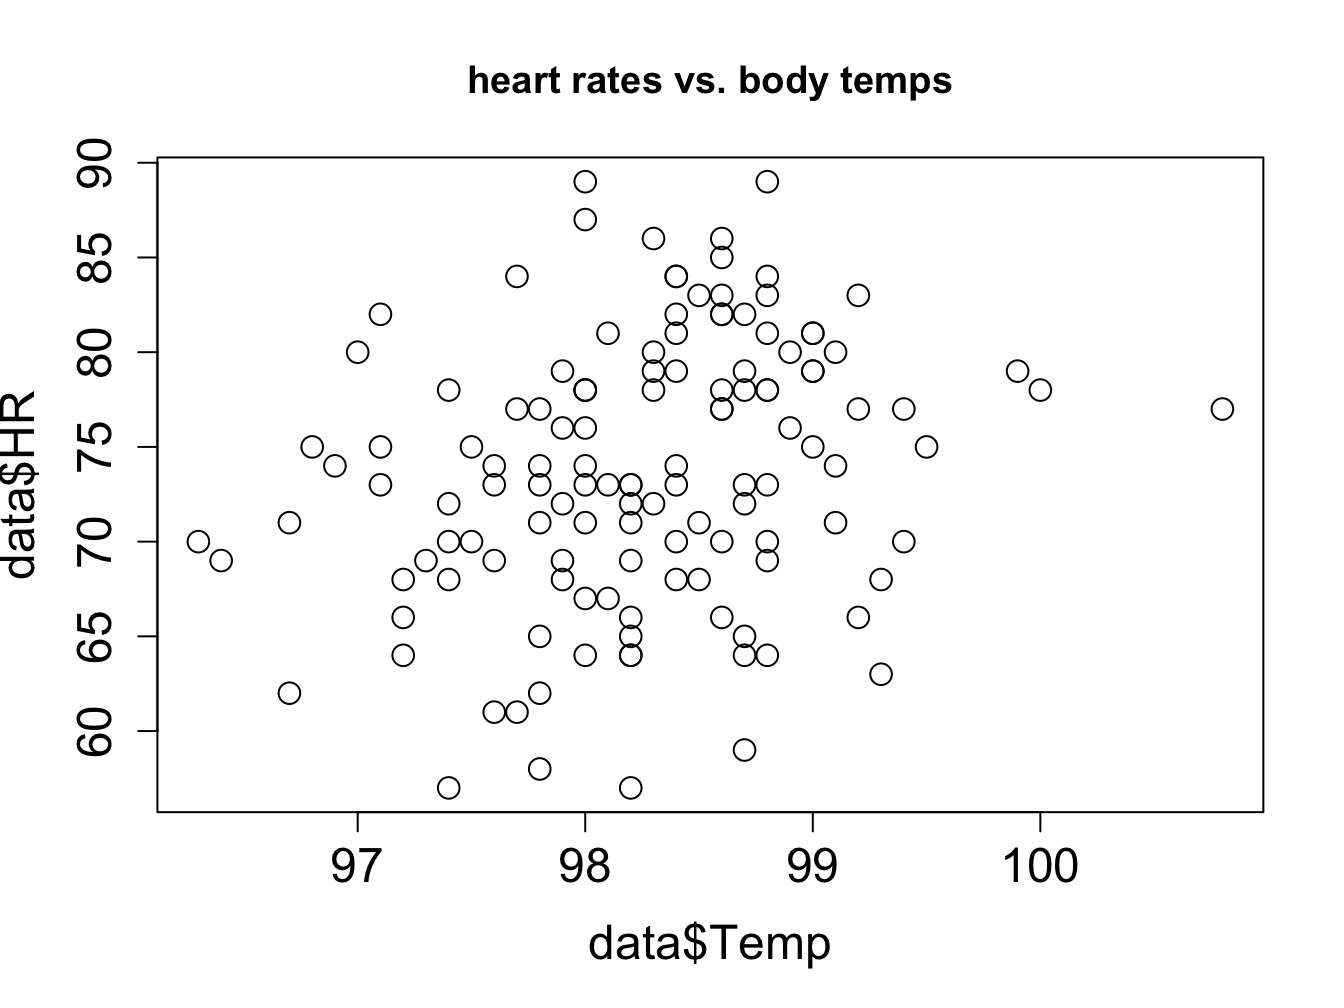
\includegraphics[width=0.5\linewidth]{QuantLife_files/figure-latex/HRTemp-scatter-1} 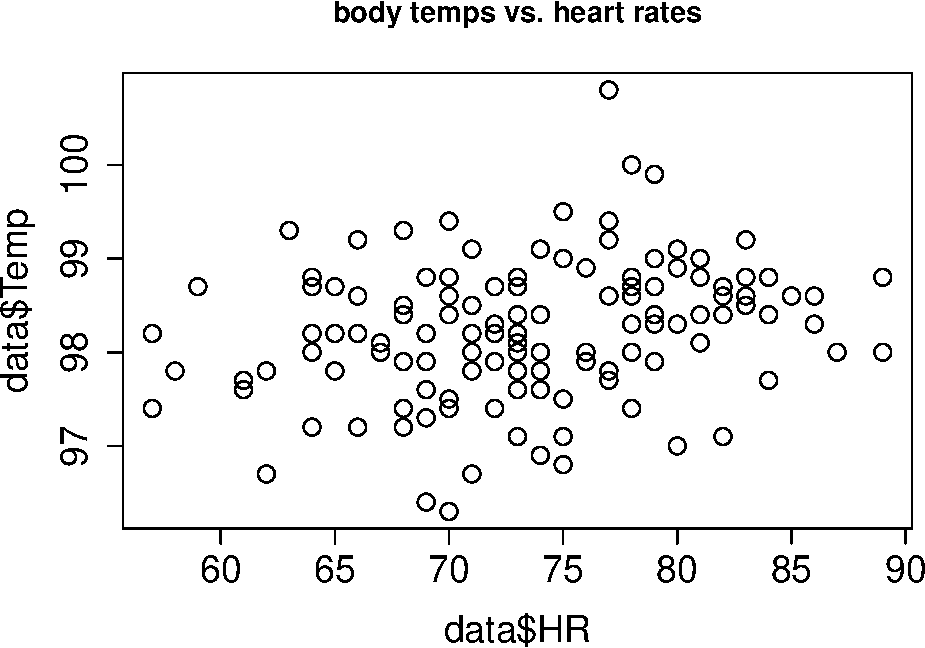
\includegraphics[width=0.5\linewidth]{QuantLife_files/figure-latex/HRTemp-scatter-2} 

}

\caption{Scatterplot of heart rates and body temperatures: a) with heart rate as the explanatory variable; b) with body temperature as the explanatory variable.}\label{fig:HRTemp-scatter}
\end{figure}

\hypertarget{linear-least-squares-fitting}{%
\section{Linear least-squares fitting}\label{linear-least-squares-fitting}}

\label{sec:math8}

\hypertarget{sum-of-squared-errors}{%
\subsection{sum of squared errors}\label{sum-of-squared-errors}}

It is easy to find the best-fit line for a data set with only two points: its slope and intercept can be found by solving the two simultaneous linear equations, e.g.~if the data set consists of \((3,2.3), (6, 1.7)\), then finding the best fit values of \(m\) and \(b\) means solving the following two equations:
\begin{eqnarray*}
3m + b &=&  2.3 \\
6m + b &=& 1.7
\end{eqnarray*}
These equations have a unique solution for each unknown: \(m=-0.2\) and \(b=2.9\) (you can solve it using basic algebra).

However, a data set with two points is very small and cannot serve as a reasonable guide for finding a relationship between two variables. Let us add one more data point, to increase our sample size to three: \((3,2.3), (6, 1.7), (9, 1.3)\). How do you find the best fit slope and intercept? \textbf{Bad idea:} take two points and find a line, that is the slope and the intercept, that passes through the two. It should be clear why this is a bad idea: we are arbitrarily ignoring some of the data, while perfectly fitting two points. So how do we use all the data? Let us write down the equations that a line with slope \(m\) and intercept \(b\) have to satisfy in order to fit our data points:
\begin{eqnarray*}
3m + b &=&  2.3 \\
6m + b &=& 1.7 \\
9m + b &=& 1.3
\end{eqnarray*}
This system has no exact solution, since there are three equations and only two unknowns. We need to find \(m\) and \(b\) such that they are a \emph{best fit} to the data, not the perfect solution. To do that, we need to define what we mean by the \index{fitting!goodness} \emph{goodness of fit}.

One simple way to asses how close the fit is to the data is to subtract the predicted values of \(y\) from the data, as follows: \(e_i = y_i - (mx_i + b)\). The values \(e_i\) are called the \emph{errors} or \index{linear regression!residual} \emph{residuals} of the linear fit. If the values predicted by the linear model (\(mx_i+b\)) are close to the actual data \(y_i\), then the error will be small. However, if we add it all up, the errors with opposite signs will cancel each other, giving the impression of a good fit simply if the deviations are symmetric.

A more reasonable approach is to take absolute values of the deviations before adding them up. This is called the total deviation, for \(n\) data points with a line fit:
\[ TD = \sum_{i=1}^n |  y_i - mx_i - b | \]

Mathematically, a better measure of total error is a sum of squared errors, which also has the advantage of adding up non-negative values, but is known as a better measure of the distance between the fit and the data (think of Euclidean distance, which is also a sum of squares) \index{fitting!least squares}:
\[ SSE = \sum_{i=1}^n ( y_i - mx_i - b )^2 \]

Thus we have formulated the goal of fitting the best line to a two-variable data set, also known as linear regression: \textbf{find the values of slope and intercept that result in the lowest possible sum of squared errors}. There is a mathematical recipe which produces these values, which will be described in the next section. Any model begins with \index{linear regression!assumptions} assumptions and in order for linear regression to be a faithful representation of a data set, the following must be true:

\begin{itemize}
\item
  the variables have a linear relationship
\item
  all of the measurements are independent of each other
\item
  there is no noise in the measurements of the explanatory variable
\item
  the noise in the measurements of the response variable is normally distributed with mean 0 and identical standard deviation
\end{itemize}

The reasons why these assumptions are necessary for linear regression to work are beyond the scope of the text, and they are elucidated very well in the book \emph{Numerical Recipes} \citep{press_numerical_2007}. However, it is important to be aware of them because if they are violated, the resulting linear fit may be meaningless. It's fairly clear that if the first assumption is violated, you are trying to impose a linear relationship on something that is actually curvy. The second assumption of independence is very important and often overlooked. The mathematical reasons for it have to do with properly measuring the goodness of fit, but intuitively it is because measurements that are linked can introduce a new relationship that has to do with the measurements, rather than the relationship between the variables. Violation of this assumption can seriously damage the reliability of the linear regression. The third assumption is often ignored, since usually the explanatory variable is also measured and thus has some noise. The reason for it is that the measure of goodness of fit is based only on the response variable, and there is no consideration of the noise in the explanatory variable. However, a reasonable amount of noise in the explanatory variable is not catastrophic for linear regression. Finally, the last assumption is due to the statistics of maximum-likelihood estimation of the slope and intercept, but again some deviation from perfect normality (bell-shaped distribution) of the noise, or slightly different variation in the noise is to be expected.

\hypertarget{best-fit-slope-and-intercept}{%
\subsection{best-fit slope and intercept}\label{best-fit-slope-and-intercept}}

\begin{definition}
\protect\hypertarget{def:def-cov}{}{\label{def:def-cov} }The \index{covariance} covariance of a data set of pairs of values \((X,Y)\) is the sum of the products of the corresponding deviations from their respective means:
\end{definition}

\[ Cov(X,Y) = \frac{1}{n-1} \sum_{i=1}^n (x_i - \bar X) (y_i - \bar Y) 
\]

Intuitively, this means that if two variable tend to deviate in the same direction from their respective means, they have a positive covariance, and if they tend to deviate in opposite directions from their means, they have a negative covariance. In the intermediate case, if sometimes they deviate together and other times they deviate in opposition, the covariance is small or zero. For instance, the covariance between two independent random variables is zero, as we saw in section \ref{sec:math4_2}.

It should come as no surprise that the slope of the linear regression depends on the covariance, that is, the degree to which the two variables deviate together from their means. If the covariance is positive, then for larger values of \(x\) the corresponding \(y\) values tend to be larger, which means the slope of the line is positive. Conversely, if the covariance is negative, so is the slope of the line. And if the two variables are independent, the slope has to be close to zero. The actual formula for the \index{linear regression!slope}\index{slope!linear regression}slope of the linear regression is \citep{whitlock_analysis_2008}:

\begin{equation}
m = \frac{Cov(X,Y)}{Var(X)}
\end{equation}

I will not provide a proof that this slope generates the minimal sum of squared errors, but that is indeed the case. To find the intercept of the linear regression, we make use of one other property of the best fit line: in order for it to minimize the SSE, it must pass through the point \((\bar X, \bar Y)\). Again, I will not prove this, but note that the point of the two mean values is the central point of the ``cloud'\,' of points in the scatterplot, and if the line missed that central point, the deviations will be larger. Assuming that is the case, we have the following equation for the line: \(\bar Y = m\bar X + b\), which we can solve for the \index{linear regression!$y$-intercept} \index{y-intercept!linear regression} intercept \(b\):
\begin{equation}
b = \bar Y - \frac{Cov(X,Y) \bar X}{Var(X)}
\end{equation}

\hypertarget{execises}{%
\subsection{Execises}\label{execises}}

\begin{longtable}[]{@{}ll@{}}
\caption{Body leanness (B) and heat loss rate (H) in boys; partial data set from \citep{sloan_cooling_1973}}\tabularnewline
\toprule
B(\(m^2/kg\)) & H(\(^\circ C /min)\)\tabularnewline
\midrule
\endfirsthead
\toprule
B(\(m^2/kg\)) & H(\(^\circ C /min)\)\tabularnewline
\midrule
\endhead
7.0 & 0.103\tabularnewline
5.0 & 0.091\tabularnewline
3.6 & 0.014\tabularnewline
3.3 & 0.024\tabularnewline
2.4 & 0.031\tabularnewline
2.1 & 0.006\tabularnewline
\bottomrule
\end{longtable}

\label{tab:ch8_bh}

Use the data set in table \ref{tab:ch8_bh} to answer the following questions:

\begin{enumerate}
\def\labelenumi{\arabic{enumi}.}
\item
  Compute the means and standard deviations of each variable.
\item
  Compute the covariance between the two variables.
\item
  Calculate the slope and intercept of the linear regression for the data with \(B\) as the explanatory variable.
\item
  Make a scatterplot of the data set with \(B\) as the explanatory variable and sketch the linear regression line with the parameters you computed.
\item
  Calculate the slope and intercept of the linear regression the data with \(H\) as the explanatory variable.
\item
  Make a scatterplot of the data set, with \(H\) as the explanatory variable and sketch the linear regression line with the parameters you computed.
\end{enumerate}

\hypertarget{correlation-and-goodness-of-fit}{%
\subsection{correlation and goodness of fit\}}\label{correlation-and-goodness-of-fit}}

The correlation between two random variables is a measure of how much variation in one corresponds to variation in the other. If this sounds very similar to the description of covariance, it's because they are closely related. Essentially, correlation is a normalized covariance, restricted to lie between -1 and 1. Here is the definition:

\begin{definition}
\protect\hypertarget{def:def-corr}{}{\label{def:def-corr} }The \index{correlation} (linear) correlation of a dataset of pairs of data values (X,Y) is:
\end{definition}
\[ r = \frac{Cov(X,Y)}{\sqrt{{Var(X)}{Var(Y)}}} =  \frac{Cov(X,Y)}{\sigma_X \sigma_Y}
\]

If the two variables are identical, \(X=Y\), then the covariance becomes its variance \(Cov(X,Y) = Var(X)\) and the denominator also becomes the variance, and the correlation is 1. This is also true if \(X\) and \(Y\) are scalar multiples of each other, as you can see by plugging in \(X= cY\) into the covariance formula. The opposite case if \(X\) and \(Y\) are diametrically opposite, \(X = -cY\), which has the correlation coefficient of -1. All other cases fall in the middle, neither perfect correlation nor perfect anti-correlation. The special case if the two variables are independent, and thus their covariance is zero, has the correlation coefficient of 0.

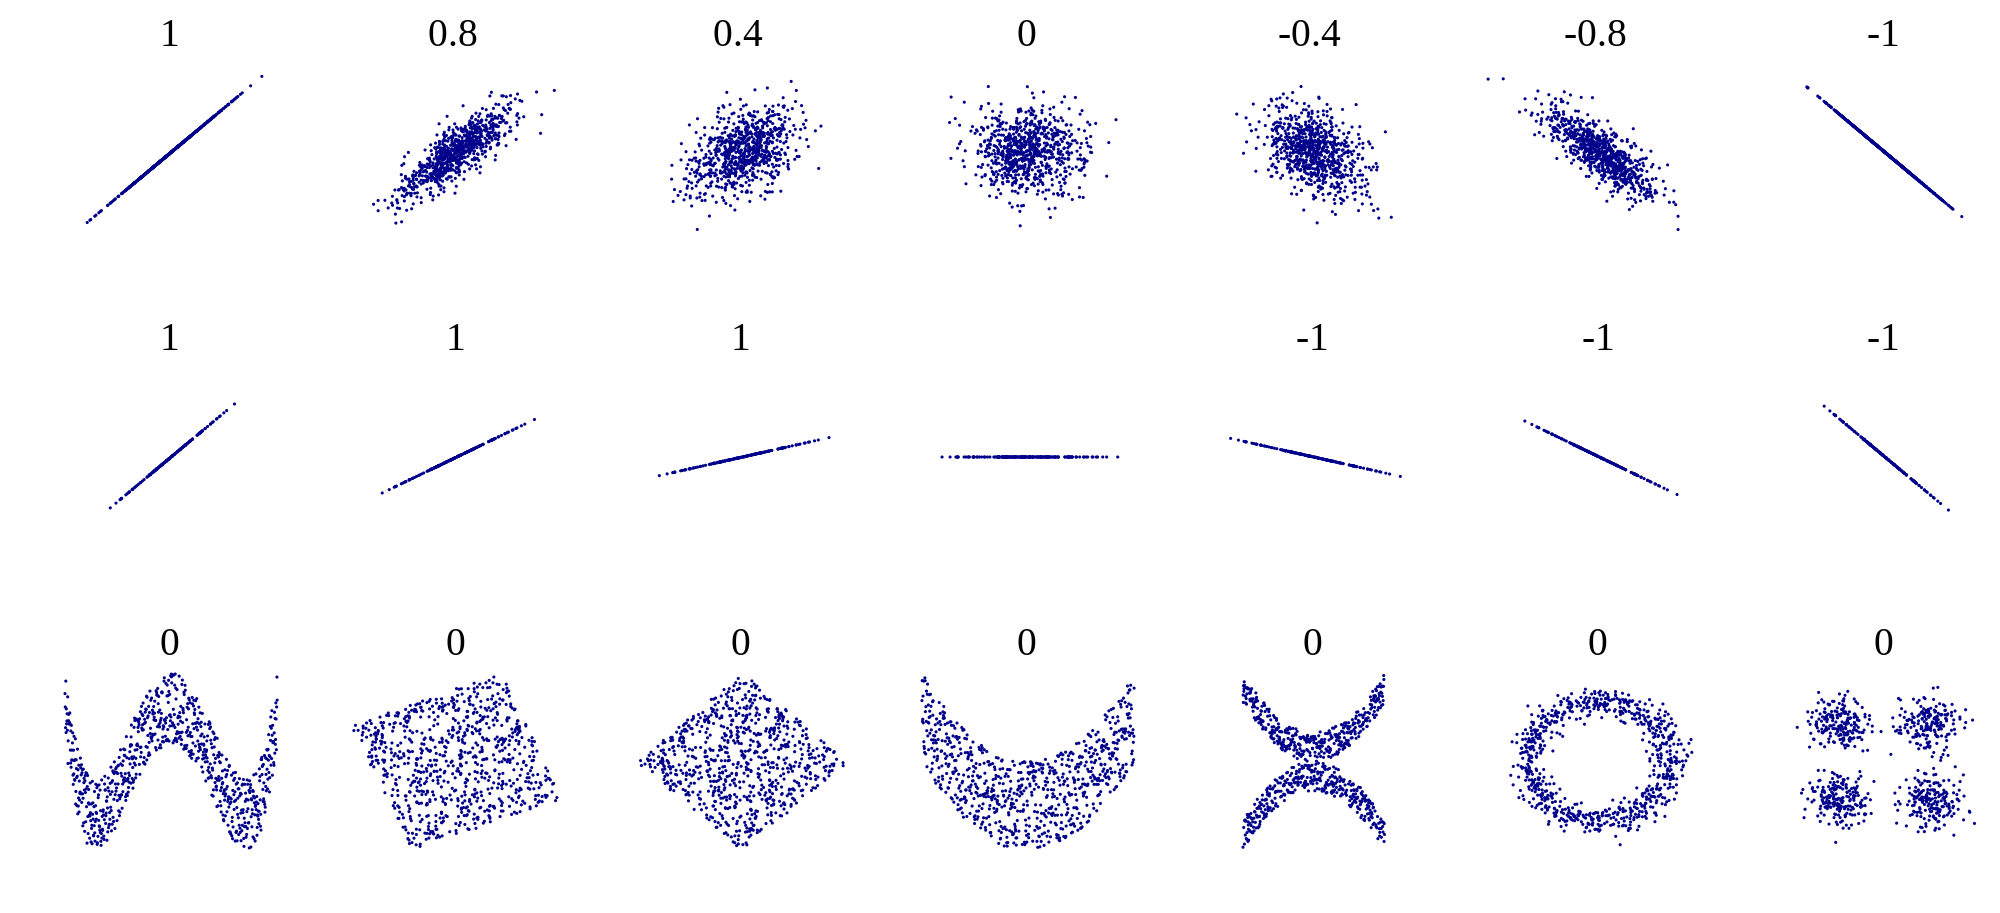
\includegraphics{ch8/Correlation_examples.png}
\label{fig:ch8_corr_examples}

This gives a connection between correlation and slope of linear regression:
\begin{equation}
m = r \frac{\sigma_Y}{\sigma_X}
\label{eq:slope_corr}
\end{equation}

Whenever linear regression is reported, one always sees the values of correlation \(r\) and squared correlation \(r^2\) displayed. The reason for this is that \(r^2\) has a very clear meaning of the \textbf{the fraction of the variance of the dependent variable \(Y\) explained by the linear regression} \(Y=mX+b\). Let us unpack what this means.

According to the stated assumptions of linear regression, the response variable \(Y\) is assumed to be linear relationship with the explanatory variable \(X\), but with independent additive noise (also normally distributed, but it doesn't play a role for this argument). Linear regression captures the linear relationship, and the remaining error (residuals) represent the noise. Thus, each value of \(Y\) can be written as \(Y = R + \hat Y\) where \(R\) is the residual (noise) and the value predicted by the linear regression is \(\hat Y =mX+b\). The assumption that \(R\) is independent of \(Y\) means that \(Var(Y) = Var (\hat Y) + Var (R)\) because variance is additive for independent random variables, as we discussed in section \ref{sec:math4}. By the same reasoning \(Cov(X,\hat Y + R) = Cov(X,\hat Y) + Cov(X,R)\). These two covariances can be simplified further: \(Cov(X,R) = 0\) because \(R\) is independent random noise. \(X\) and the predicted \(\hat Y\) are perfectly correlated, so \(Cov(X,\hat Y) = Cov(X,mX+b) = Var(X) = Var(\hat Y)\). This leads to the derivation of the meaning of \(r^2\):

\begin{equation}
\begin{aligned}
  r^2 = \frac{Cov(X,Y)^2}{Var(X) Var(Y)} &=   \frac{(Cov(X,\hat Y) + Cov(X,R) )^2}{Var(X) Var(Y)}   = \\
  =\frac{Var(X)Var(\hat Y)}{Var(X) Var(Y)} &=  \frac{Var(\hat Y)}{Var(Y)}
  \end{aligned}
\label{eq:ch8_frac_var}
\end{equation}

One should be cautious when interpreting results of a linear regression. First, just because there is no linear relationship does not mean that there is no other relationship. Figure \ref{fig:ch8_corr_examples} shows some examples of scatterplots and their corresponding correlation coefficients. What it shows is that while a formless blob of a scatterplot will certainly have zero correlation, so will other scatterplots in which there is a definite relationship (e.g.~a circle, or a X-shape). The point is that \textbf{correlation is always a measure of the linear relationship between variables.}

The second caution is well known, as that is the danger of equating correlation with a causal relationship. There are numerous examples of scientists misinterpreting a coincidental correlation as meaningful, or deeming two variables that have a common source as causing one another. For example, one can look at the increase in automobile ownership in the last century and the concurrent improvement in longevity and conclude that automobiles are good for human health. It is well-documented, however, that a sedentary lifestyle and automobile exhaust do not make a person healthy. Instead, increased prosperity has increased both the purchasing power of individuals and enabled advances in medicine that have increase our lifespans. To summarize, one must be careful when interpreting correlation: a weak one does not mean there is no relationship, and a strong one does not mean that one variable causes the changes in the other.

There is another important measure of the quality of linear regression: the \index{plot!residual}\index{linear regression!residual} residual plot. The residuals are the differences between the predicted values of the response variable and the actual value from the data. As stated above, linear regression assumes that there is a linear relationship between the two variables, plus some uncorrelated noise added to the values of the response variable. If that were true, then the plot of the residuals would look like a vaguely spherical blob, with a mean value of 0 and no discernible trend (e.g.~no increase of residual for larger \(x\) values). Visually assessing residual plots is an essential check on whether linear regression is a reasonable fit to the data in addition to the \(r^2\) value.

\hypertarget{exercises-10}{%
\subsection{Exercises}\label{exercises-10}}

Figure \ref{fig:ch8_penguins} shows scatterplots of the rate of oxygen consumption (VO) and heart rate (HR) measured in two macaroni penguins running on a treadmill (really). The authors performed linear regression on the data and found the following parameters: \(VO =0.23HR - 11.62\) (penguin A) and \(VO =0.25HR - 20.93\) (penguin B). The datasets have the standard deviations: \(\sigma_{VO} = 6.77\) and \(\sigma_{HR} = 28.8\) (penguin A) and \(\sigma_{VO} = 8.49\) and \(\sigma_{HR} = 30.6\) (penguin B).

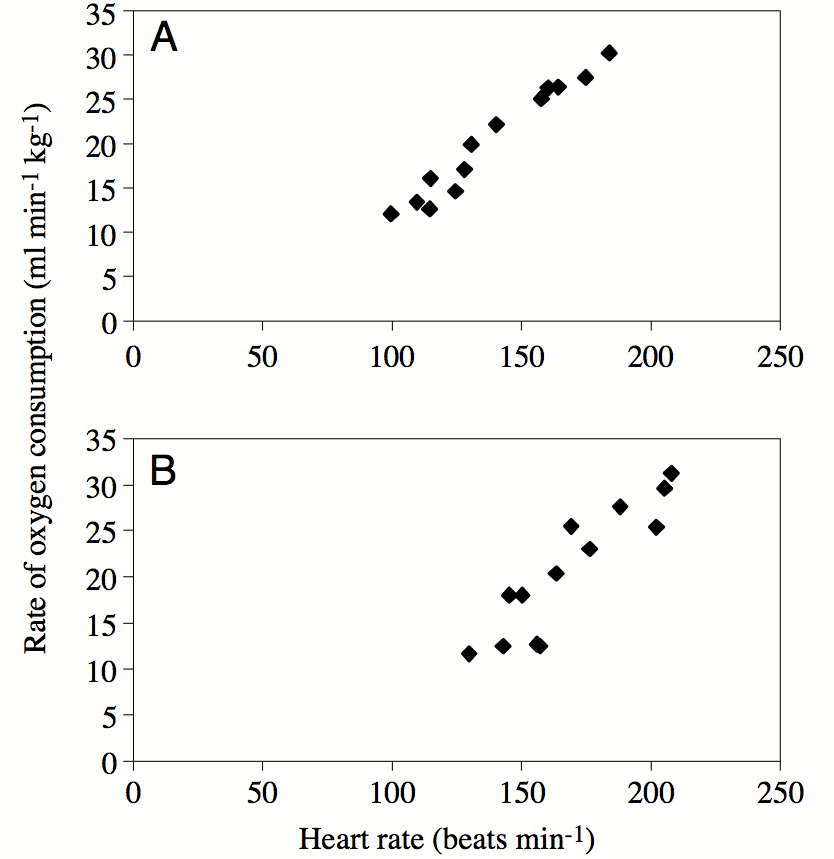
\includegraphics{ch8/penguin_HR.png}
\label{fig:ch8_penguins}

\begin{enumerate}
\def\labelenumi{\arabic{enumi}.}
\item
  Find the dimensions and units of the slope and the intercept of the linear regression for this data (the units of HR and VO are on the plot).
\item
  Data set B has a larger slope than data set A. Does this mean the correlation is higher in data set B than in A? Explain.
\item
  Calculate the correlation coefficients for the linear regressions of the two penguins; explain how much variance is explained in each case.
\item
  Re-calculate the slopes of the two linear regressions if the explanatory and response variables were reversed. Does changing the order of variable affect the correlation?
\end{enumerate}

\hypertarget{linear-regression-using-r}{%
\section{Linear regression using R}\label{linear-regression-using-r}}

\label{sec:comp6}

We now have the tools to compute the parameters of the best-fit line, provided we can calculate the means, variances, and covariance of the two variable data set. Of course, the best way to do all this is to let a computer handle it. The function for calculating linear regression in R is \texttt{lm()}, which outputs a bunch of information to a variable called myfit in the script below. The slope, intercept, and other \index{parameter!linear regression}parameters can be printed out using the \texttt{summary()} function. In the script below you see a bunch of information, but we are concerned with the ones in the first column correspond to the best fit intercept (-166.2847) and the slope (2.4432). You can check that they correspond to our formulas by computing the covariance, the variances, and the means of the two variables:

\begin{Shaded}
\begin{Highlighting}[]
\NormalTok{my\_data \textless{}{-}}\StringTok{ }\KeywordTok{read.table}\NormalTok{(}\StringTok{"data/HR\_temp.txt"}\NormalTok{, }\DataTypeTok{header =} \OtherTok{TRUE}\NormalTok{)}
\NormalTok{myfit \textless{}{-}}\StringTok{ }\KeywordTok{lm}\NormalTok{(HR }\OperatorTok{\textasciitilde{}}\StringTok{ }\NormalTok{Temp, my\_data)}
\KeywordTok{summary}\NormalTok{(myfit)}
\end{Highlighting}
\end{Shaded}

\begin{verbatim}
## 
## Call:
## lm(formula = HR ~ Temp, data = my_data)
## 
## Residuals:
##      Min       1Q   Median       3Q      Max 
## -16.6413  -4.6356   0.3247   4.8304  15.8474 
## 
## Coefficients:
##              Estimate Std. Error t value Pr(>|t|)   
## (Intercept) -166.2847    80.9123  -2.055  0.04190 * 
## Temp           2.4432     0.8235   2.967  0.00359 **
## ---
## Signif. codes:  0 '***' 0.001 '**' 0.01 '*' 0.05 '.' 0.1 ' ' 1
## 
## Residual standard error: 6.858 on 128 degrees of freedom
## Multiple R-squared:  0.06434,    Adjusted R-squared:  0.05703 
## F-statistic: 8.802 on 1 and 128 DF,  p-value: 0.003591
\end{verbatim}

\begin{Shaded}
\begin{Highlighting}[]
\NormalTok{m \textless{}{-}}\StringTok{ }\KeywordTok{cov}\NormalTok{(my\_data}\OperatorTok{$}\NormalTok{HR, my\_data}\OperatorTok{$}\NormalTok{Temp)}\OperatorTok{/}\KeywordTok{var}\NormalTok{(my\_data}\OperatorTok{$}\NormalTok{Temp)}
\KeywordTok{print}\NormalTok{(m)}
\end{Highlighting}
\end{Shaded}

\begin{verbatim}
## [1] 2.443238
\end{verbatim}

\begin{Shaded}
\begin{Highlighting}[]
\NormalTok{b \textless{}{-}}\StringTok{ }\KeywordTok{mean}\NormalTok{(my\_data}\OperatorTok{$}\NormalTok{HR) }\OperatorTok{{-}}\StringTok{ }\NormalTok{m }\OperatorTok{*}\StringTok{ }\KeywordTok{mean}\NormalTok{(my\_data}\OperatorTok{$}\NormalTok{Temp)}
\KeywordTok{print}\NormalTok{(b)}
\end{Highlighting}
\end{Shaded}

\begin{verbatim}
## [1] -166.2847
\end{verbatim}

Here \texttt{Temp} and \texttt{HR} are the explanatory and response variables, respectively, and \texttt{my\_data} is the name of the data frame they are stored in. The best fit parameters are stored in \texttt{myfit}, and the line can be plotted using \texttt{abline(myfit)}. The script below shows how to calculate a linear regression line and then plot it over a scatterplot in R, and the result is shown in figure \ref{fig:linreg_HRTemp}a.

\begin{Shaded}
\begin{Highlighting}[]
\KeywordTok{plot}\NormalTok{(my\_data}\OperatorTok{$}\NormalTok{Temp, my\_data}\OperatorTok{$}\NormalTok{HR, }\DataTypeTok{main =} \StringTok{"scatterplot and linear regression line"}\NormalTok{, }
    \DataTypeTok{cex =} \FloatTok{1.5}\NormalTok{, }\DataTypeTok{cex.axis =} \FloatTok{1.5}\NormalTok{, }\DataTypeTok{cex.lab =} \FloatTok{1.5}\NormalTok{)}
\KeywordTok{abline}\NormalTok{(myfit)}
\NormalTok{HRresiduals \textless{}{-}}\StringTok{ }\KeywordTok{resid}\NormalTok{(myfit)}
\KeywordTok{plot}\NormalTok{(data}\OperatorTok{$}\NormalTok{Temp, HRresiduals, }\DataTypeTok{main =} \StringTok{"residuals plot"}\NormalTok{, }
    \DataTypeTok{cex =} \FloatTok{1.5}\NormalTok{, }\DataTypeTok{cex.axis =} \FloatTok{1.5}\NormalTok{, }\DataTypeTok{cex.lab =} \FloatTok{1.5}\NormalTok{)}
\KeywordTok{abline}\NormalTok{(}\DecValTok{0}\NormalTok{, }\DecValTok{0}\NormalTok{)}
\end{Highlighting}
\end{Shaded}

\begin{figure}

{\centering 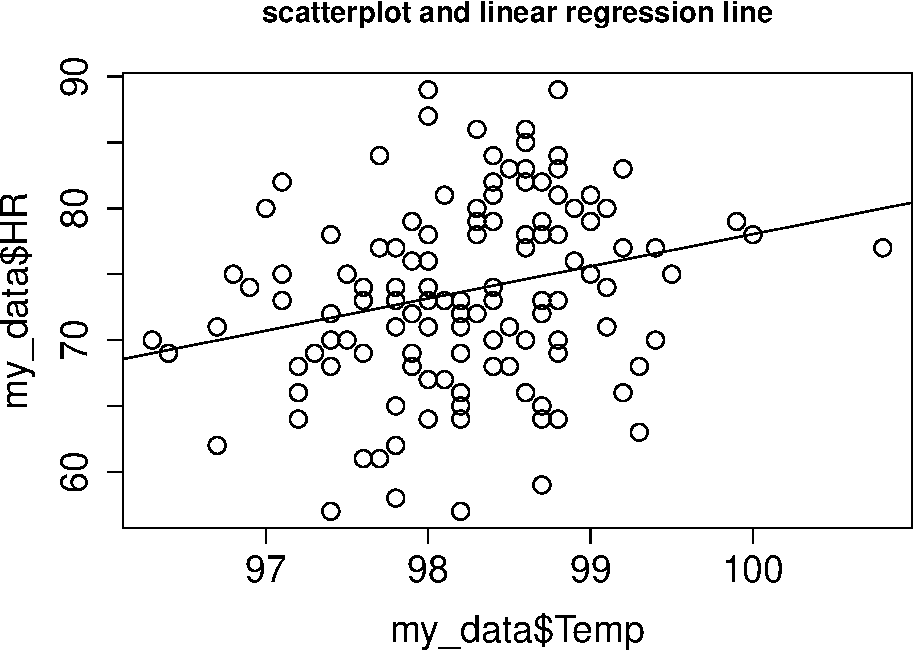
\includegraphics[width=0.5\linewidth]{QuantLife_files/figure-latex/linreg-HRTemp-1} 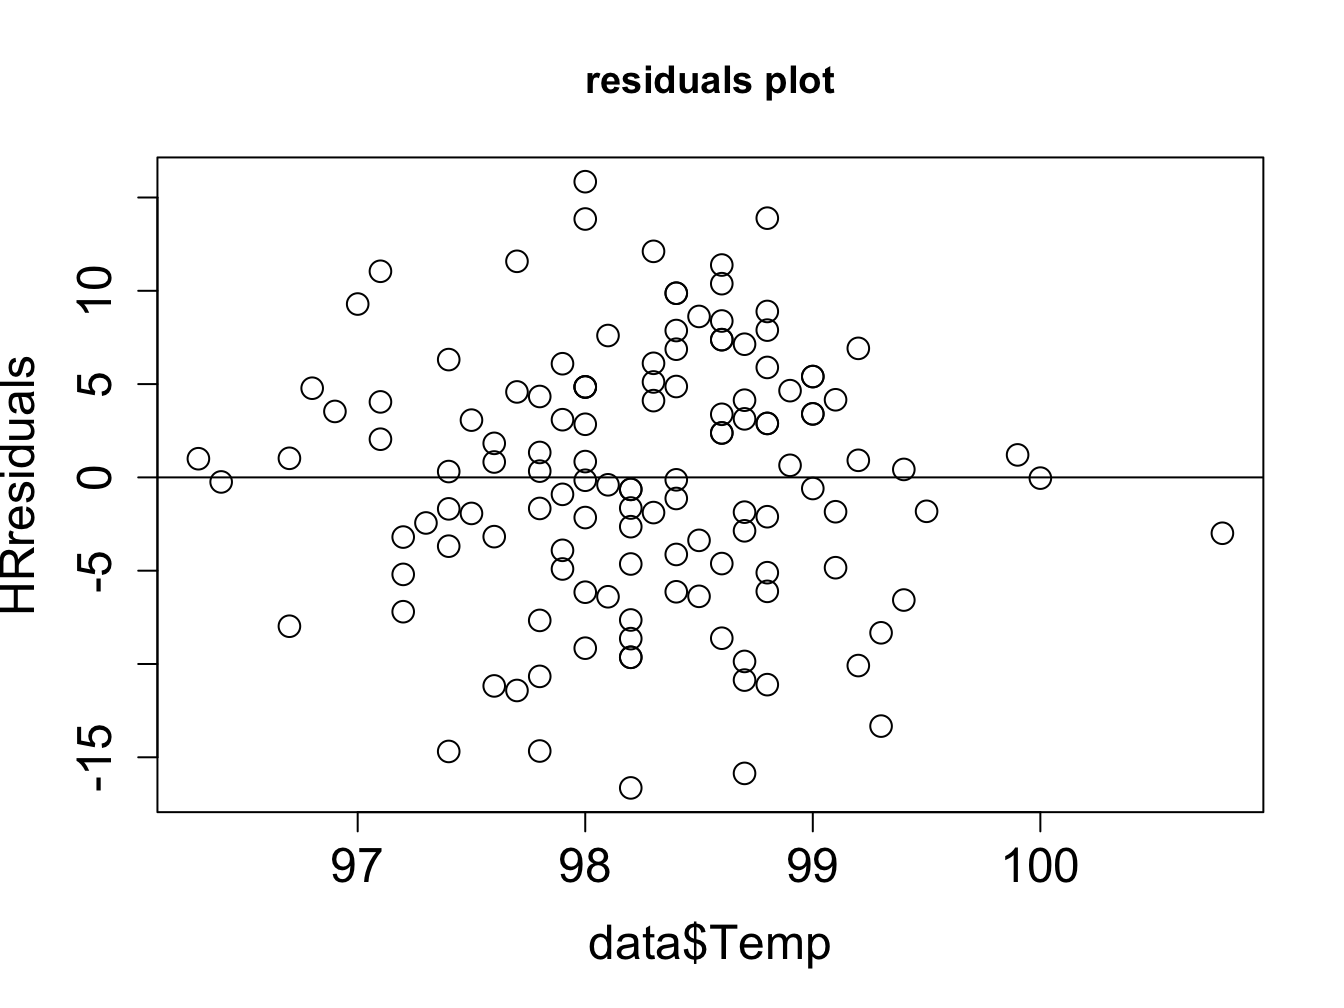
\includegraphics[width=0.5\linewidth]{QuantLife_files/figure-latex/linreg-HRTemp-2} 

}

\caption{Linear regression for a data set of heart rates and body temperatures (a); and the residuals (b).}\label{fig:linreg-HRTemp}
\end{figure}

However, what does this mean about the quality of the fit? Just because we found a line to draw through a scatterplot does not mean that this line is meaningful. In fact, looking at the plot, there does not seem to be much of a relationship between the two variables. There are various statistical measures for the significance of linear regression, the most important one relies on the correlation between the two data sets. Look again at the summary statistics for the data set of heart rates and temperatures. There are several different statistics here, and the one that we care about is the \(r^2\), which is reported here as `Multiple R-squared'. This number tells us that the linear regression accounts for only about 6\% of the total variance of the heart rate. In other words, there is no significant linear relationship in this data set.

As mentioned in section \ref{sec:math8}, the other important check is plotting the residuals of the data set, after the linear fit is subtracted. You see the result in figure \ref{fig:linreg_HRTemp}b, showing that the residuals do not have any pronounced pattern. So it is reasonable to conclude that linear regression was a reasonable model to which to fit the data. The low correlation is because data seem to have little to no relationship, not because there is some complicated nonlinear relationship.

Here is an example of a linear regression performed and the line plotted over the basic R plot. Note that lm() uses the following syntax to indicate which variable is which: lm(Y \textasciitilde{} X) (where Y is the response variable and X is the explanatory variable.)

\begin{Shaded}
\begin{Highlighting}[]
\NormalTok{myfit \textless{}{-}}\StringTok{ }\KeywordTok{lm}\NormalTok{(child }\OperatorTok{\textasciitilde{}}\StringTok{ }\NormalTok{parent, Galton) }
\KeywordTok{summary}\NormalTok{(myfit)}
\end{Highlighting}
\end{Shaded}

\begin{verbatim}
## 
## Call:
## lm(formula = child ~ parent, data = Galton)
## 
## Residuals:
##     Min      1Q  Median      3Q     Max 
## -7.8050 -1.3661  0.0487  1.6339  5.9264 
## 
## Coefficients:
##             Estimate Std. Error t value Pr(>|t|)    
## (Intercept) 23.94153    2.81088   8.517   <2e-16 ***
## parent       0.64629    0.04114  15.711   <2e-16 ***
## ---
## Signif. codes:  0 '***' 0.001 '**' 0.01 '*' 0.05 '.' 0.1 ' ' 1
## 
## Residual standard error: 2.239 on 926 degrees of freedom
## Multiple R-squared:  0.2105, Adjusted R-squared:  0.2096 
## F-statistic: 246.8 on 1 and 926 DF,  p-value: < 2.2e-16
\end{verbatim}

\begin{Shaded}
\begin{Highlighting}[]
\KeywordTok{print}\NormalTok{(}\KeywordTok{paste}\NormalTok{(}\StringTok{"The best{-}fit slope is: "}\NormalTok{, myfit}\OperatorTok{$}\NormalTok{coefficients[}\DecValTok{2}\NormalTok{]))}
\end{Highlighting}
\end{Shaded}

\begin{verbatim}
## [1] "The best-fit slope is:  0.646290581993716"
\end{verbatim}

\begin{Shaded}
\begin{Highlighting}[]
\KeywordTok{print}\NormalTok{(}\KeywordTok{paste}\NormalTok{(}\StringTok{"The best{-}fit intercept is: "}\NormalTok{, myfit}\OperatorTok{$}\NormalTok{coefficients[}\DecValTok{1}\NormalTok{]))      }
\end{Highlighting}
\end{Shaded}

\begin{verbatim}
## [1] "The best-fit intercept is:  23.9415301804085"
\end{verbatim}

The summary outputs a whole bunch of information that is returned by the \texttt{lm()} function, as the object \texttt{myfit}. The most important are the intercept and slope, which may be printed out as shown above, and the R-squared parameter, also called the coefficient of determination. The value of R-squared is not accessible directly in \texttt{myfit}, but it is printed out in the summary (use multiple R-squared for our assignments.)

The actual best-fit line can be plotted as follows over a scatterplot of the data; notice that abline can take myfit as an input and use the slope and intercept:

\begin{Shaded}
\begin{Highlighting}[]
\CommentTok{\#Overlay the best{-}fit line on the base R plot}
\KeywordTok{plot}\NormalTok{(Galton}\OperatorTok{$}\NormalTok{parent, Galton}\OperatorTok{$}\NormalTok{child, }\DataTypeTok{xlab=}\StringTok{\textquotesingle{}mid{-}parent height (inches)\textquotesingle{}}\NormalTok{, }\DataTypeTok{ylab=}\StringTok{\textquotesingle{}child height (inches)\textquotesingle{}}\NormalTok{)}
\KeywordTok{abline}\NormalTok{(myfit)}
\end{Highlighting}
\end{Shaded}

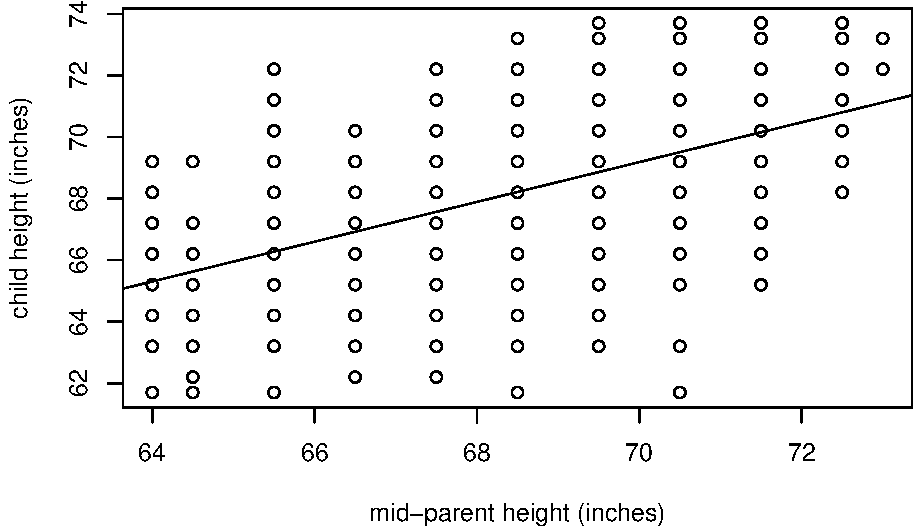
\includegraphics{QuantLife_files/figure-latex/unnamed-chunk-78-1.pdf}

After performing linear regression it is essential to check that the residuals obey the assumptions of linear regression. The residuals are the difference between the predicted response variable values and the actual values of the response variable, in this case the child height. The residuals are contained in the object myfit as variable residuals:

\begin{Shaded}
\begin{Highlighting}[]
\KeywordTok{plot}\NormalTok{(Galton}\OperatorTok{$}\NormalTok{parent, myfit}\OperatorTok{$}\NormalTok{residuals, }\DataTypeTok{xlab=}\StringTok{\textquotesingle{}mid{-}parent height (inches)\textquotesingle{}}\NormalTok{, }\DataTypeTok{ylab=}\StringTok{\textquotesingle{}residuals (inches)\textquotesingle{}}\NormalTok{)}
\KeywordTok{abline}\NormalTok{(}\DecValTok{0}\NormalTok{,}\DecValTok{0}\NormalTok{)}
\end{Highlighting}
\end{Shaded}

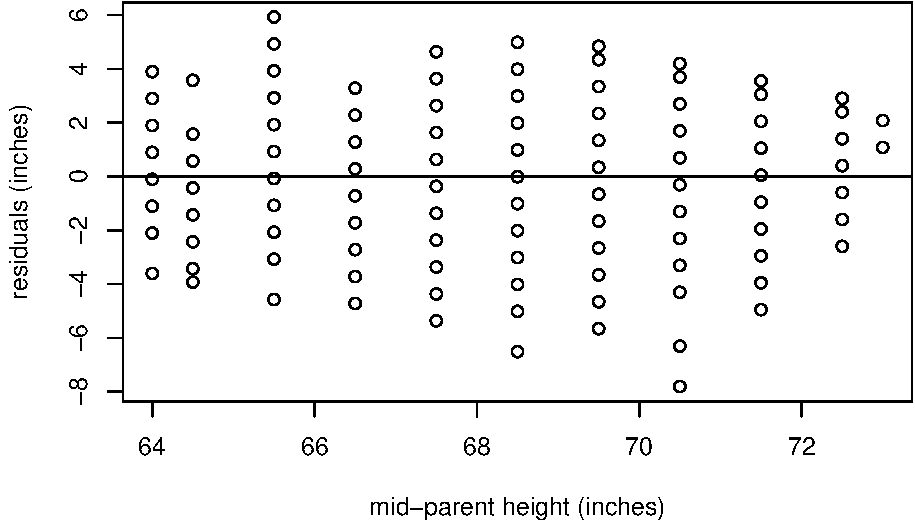
\includegraphics{QuantLife_files/figure-latex/unnamed-chunk-79-1.pdf}

It appears that the residuals meet the assumptions of being independent of measurement (shapeless scatterplot), are centered at zero, and look roughly normally distributed, although that can be checked more carefully using other tools.

\hypertarget{exercises-11}{%
\subsection{Exercises:}\label{exercises-11}}

\begin{enumerate}
\def\labelenumi{\arabic{enumi}.}
\item
  Calculate descriptive statistics (mean and standard deviation) of the residuals from the linear regression above. What do you expect them to be, and how do they differ from the expectation? Using this calculation, check that the coefficient of determination really captures the fraction of total variance explained by linear regression
\item
  Perform linear regression on the Galton data set with the response and explanatory variables switched, and report which parameters changed and how.
\item
  Plot the residuals from your new linear regression and calculate and report their descriptive statistics. What do you expect them to be, and how do they differ from the expectation? Using this calculation, check that the coefficient of determination really captures the fraction of total variance explained by linear regression.
\end{enumerate}

\hypertarget{regression-to-the-mean}{%
\section{Regression to the mean}\label{regression-to-the-mean}}

\label{sec:bio8}
The phenomenon called \index{regression to the mean} regression to the mean is initially surprising. Francis Galton first discovered this by comparing the heights of parents and their offspring. Galton took a subset of parents who are taller than average and observed that their children were, on average, shorter than their parents. He also compared the heights of parents who are shorter than average, and found that their children were on average taller than their parents. This suggests the conclusion that in long run everyone will converge closer to the average height - hence ``regression to mediocrity'', as Galton called it \citep{senn_francis_2011}.

\begin{Shaded}
\begin{Highlighting}[]
\KeywordTok{library}\NormalTok{(}\StringTok{"HistData"}\NormalTok{)}
\NormalTok{myfit \textless{}{-}}\StringTok{ }\KeywordTok{lm}\NormalTok{(child }\OperatorTok{\textasciitilde{}}\StringTok{ }\NormalTok{parent, Galton)}
\KeywordTok{plot}\NormalTok{(Galton}\OperatorTok{$}\NormalTok{parent, Galton}\OperatorTok{$}\NormalTok{child, }\DataTypeTok{xlab =} \StringTok{"mid{-}parent height (inches)"}\NormalTok{, }
    \DataTypeTok{ylab =} \StringTok{"child height (inches)"}\NormalTok{, }\DataTypeTok{cex =} \FloatTok{1.5}\NormalTok{, }\DataTypeTok{cex.axis =} \FloatTok{1.5}\NormalTok{, }
    \DataTypeTok{cex.lab =} \FloatTok{1.5}\NormalTok{)}
\KeywordTok{abline}\NormalTok{(myfit, }\DataTypeTok{lwd =} \DecValTok{3}\NormalTok{, }\DataTypeTok{lty =} \DecValTok{1}\NormalTok{)}
\KeywordTok{abline}\NormalTok{(}\DecValTok{0}\NormalTok{, }\DecValTok{1}\NormalTok{, }\DataTypeTok{lwd =} \DecValTok{3}\NormalTok{, }\DataTypeTok{lty =} \DecValTok{2}\NormalTok{, }\DataTypeTok{col =} \StringTok{"red"}\NormalTok{)}
\NormalTok{myfit \textless{}{-}}\StringTok{ }\KeywordTok{lm}\NormalTok{(parent }\OperatorTok{\textasciitilde{}}\StringTok{ }\NormalTok{child, Galton)}
\KeywordTok{plot}\NormalTok{(Galton}\OperatorTok{$}\NormalTok{child, Galton}\OperatorTok{$}\NormalTok{parent, }\DataTypeTok{xlab =} \StringTok{"child height (inches)"}\NormalTok{, }
    \DataTypeTok{ylab =} \StringTok{"mid{-}parent height (inches)"}\NormalTok{, }\DataTypeTok{cex =} \FloatTok{1.5}\NormalTok{, }
    \DataTypeTok{cex.axis =} \FloatTok{1.5}\NormalTok{, }\DataTypeTok{cex.lab =} \FloatTok{1.5}\NormalTok{)}
\KeywordTok{abline}\NormalTok{(myfit, }\DataTypeTok{lwd =} \DecValTok{3}\NormalTok{)}
\KeywordTok{abline}\NormalTok{(}\DecValTok{0}\NormalTok{, }\DecValTok{1}\NormalTok{, }\DataTypeTok{lwd =} \DecValTok{3}\NormalTok{, }\DataTypeTok{lty =} \DecValTok{2}\NormalTok{, }\DataTypeTok{col =} \StringTok{"red"}\NormalTok{)}
\end{Highlighting}
\end{Shaded}

\begin{figure}

{\centering 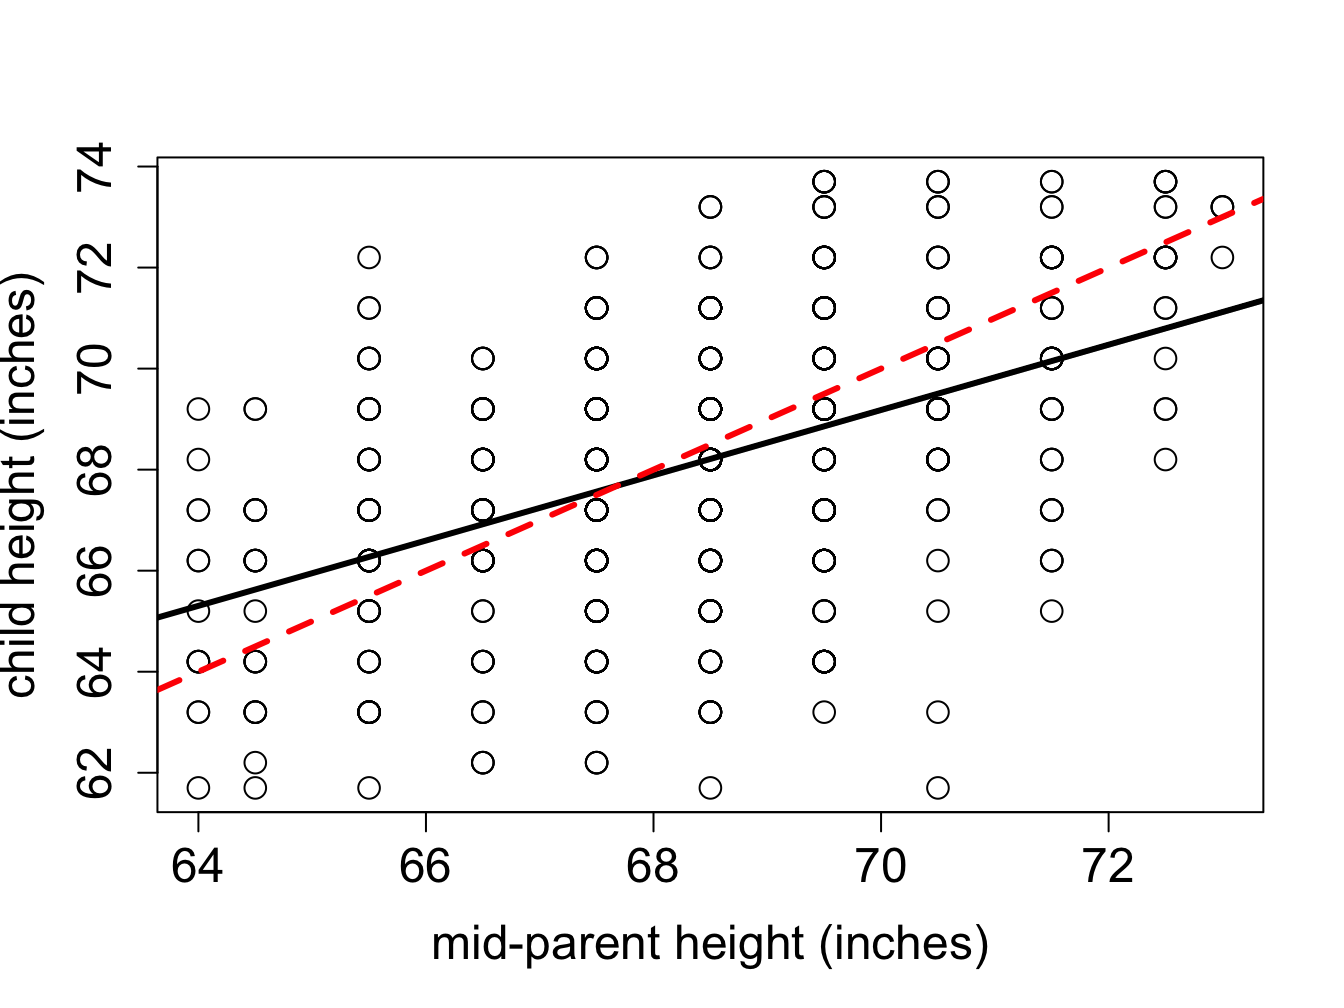
\includegraphics[width=0.5\linewidth]{QuantLife_files/figure-latex/linreg-Galton-1} 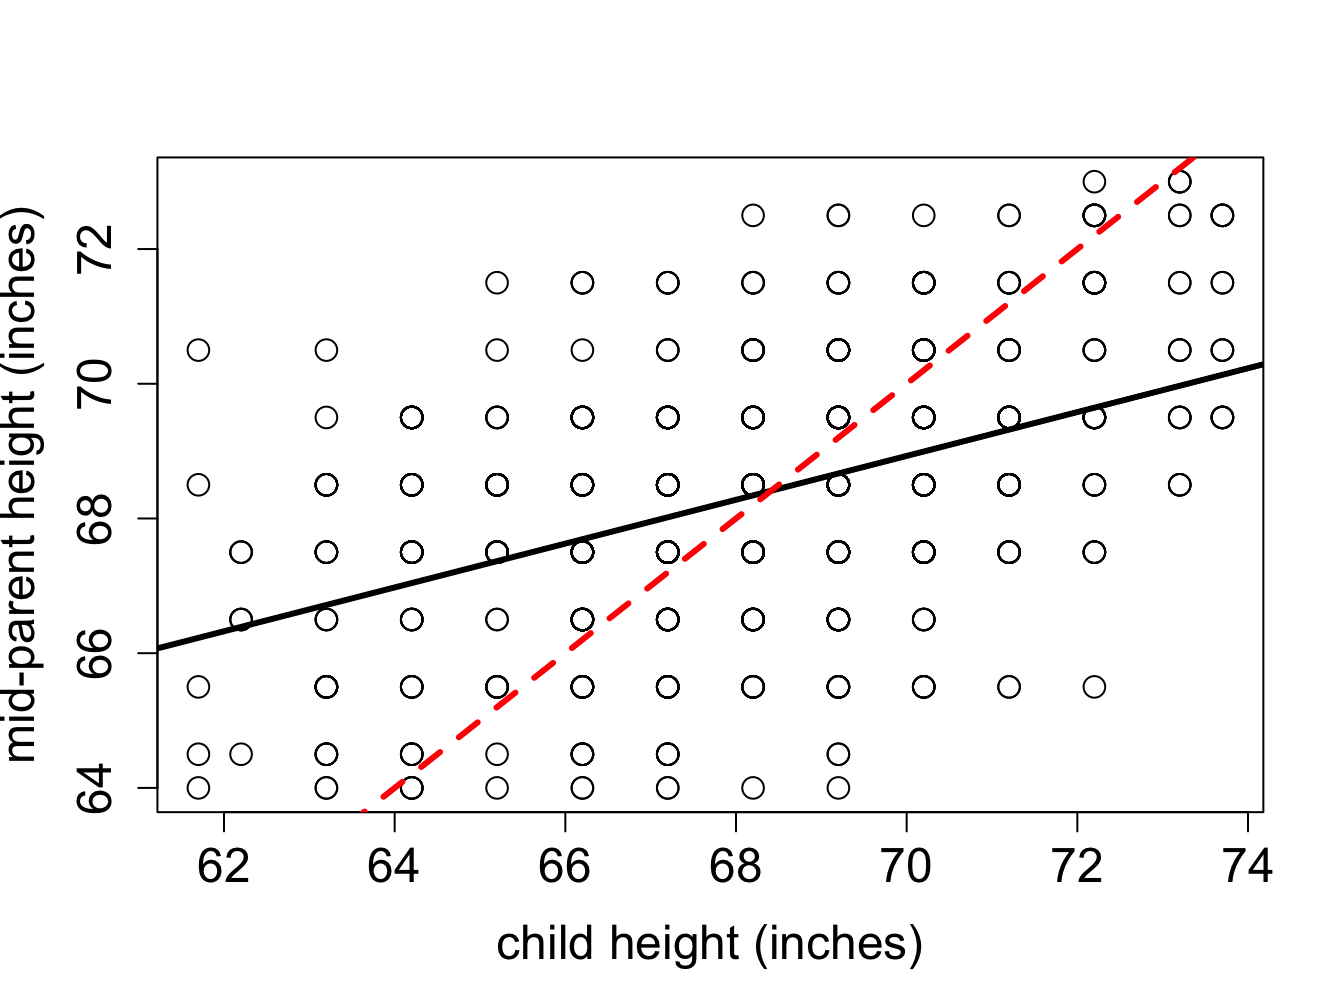
\includegraphics[width=0.5\linewidth]{QuantLife_files/figure-latex/linreg-Galton-2} 

}

\caption{Galton data on heights of parents and of children as scatterplots (two versions with explanatory and response variables switched). The dotted red lines show the identity line y=x and the solid black line is the linear regression.}\label{fig:linreg-Galton}
\end{figure}

But that is not the case! The parents and children in Galton's experiment had a very similar mean and standard deviation. This appears to be a paradox, but it is easily explained using linear regression. Consider two identically distributed random variables \((X,Y)\) with a positive correlation \(r\). The slope of the linear regression is \(m = r \sigma_Y/\sigma_X\) and since \(\sigma_Y=\sigma_X\), the slope is simply \(r\). Select a subset with values of \(X\) higher than \(\bar X\), and consider the mean value of \(Y\) for that subset. If the slope \(m<1\) (the correlation is not perfect), then the mean value of \(Y\) for that subset is less than the mean value of \(X\). Similarly, for a subset with values of \(X\) lower than \(\bar X\), the mean value of \(Y\) for that subset is greater than the mean value of \(X\), again as long as the slope is less than 1.

Figure \ref{fig:regression2mean} shows Galton's data set (available in R by installing the package `HistData') along with the linear regression line and the identity like (\(y=x\)). If each child had exactly the same height as the parents, the scatterplot would lie on the identity line. Instead, the linear regression lines have slope less than 1 for both the plot with the parental heights as the explanatory variable and for the plot with the variables reversed. The correlation coefficient \(r\) does not depend on the order of the variables; so using the equation \ref{eq:slope_corr} we can see the difference in slopes is explained by the two data sets having different standard deviations, and reversing the explanatory and response variables results in reciprocation of the ratio of standard deviations. The children's heights have a higher standard deviation, which is likely an artifact of the experiment. In the data set the heights of the two parents were averaged to take them both into account, which substantially reduces the spread between male and female heights. To summarize, although the children of taller parents are shorter on average than their parents, and the children of shorter parents are taller than their parents, the overall standard deviation does not decrease from generation to generation.

\hypertarget{discussion-questions-1}{%
\subsection{Discussion questions}\label{discussion-questions-1}}

Please read the paper on measuring the rate of \index{sequencing!whole genome} de novo mutations in humans and its relationship to paternal age \citep{kong_rate_2012}.

\begin{enumerate}
\def\labelenumi{\arabic{enumi}.}
\item
  What types of mutations were observed in the data set? What were the most and the least common?
\item
  The paper shows that both maternal and paternal age are positively correlated with offspring inheriting new mutations. What biological mechanism explains why paternal age is the dominant factor? What could explain the substantial correlation with maternal age?
\item
  Is linear regression the best representation of the relationship between paternal age and number of mutations? What other model did the authors use to fit the data, and how did it perform?
\item
  What do you make of the historical data of paternal ages the authors present at the end of the paper? Can you postulate a testable hypothesis based on this observation?
\end{enumerate}

\hypertarget{r-assignment-3}{%
\section{R Assignment}\label{r-assignment-3}}

In each of the following questions, do these tasks:

\begin{enumerate}
\def\labelenumi{\arabic{enumi})}
\tightlist
\item
  calculate the linear regression on the indicated variables in the data set
\item
  plot the scatterplot and overlay the linear regression line
\item
  plot the residuals as a function of the explanatory variable
\item
  answer questions about interpretation of linear regression
\end{enumerate}

\begin{enumerate}
\def\labelenumi{\arabic{enumi}.}
\item
  \begin{enumerate}
  \def\labelenumii{\alph{enumii})}
  \tightlist
  \item
    Use the data from the file \texttt{kong\_mutation\_data.txt} and perform the tasks stated above for Mutations as a function of PatAge (remember to label your plots and axes!)
  \end{enumerate}
\end{enumerate}

\begin{Shaded}
\begin{Highlighting}[]
\CommentTok{\# YOUR CODE HERE}
\end{Highlighting}
\end{Shaded}

How does the slope compare to the fit your performed by eye in question 1.1a? What does the slope of that line mean? What fraction of the variance is explained by the linear relationship? Does the plot of residuals show any significant deviations from the assumptions?

YOUR ANSWERS GO HERE

\begin{enumerate}
\def\labelenumi{\alph{enumi})}
\setcounter{enumi}{1}
\tightlist
\item
  Perform the same tasks as above for \texttt{Mutations} as a function of \texttt{MatAge} (remember to label your plots and axes!)
\end{enumerate}

\begin{Shaded}
\begin{Highlighting}[]
\CommentTok{\# YOUR CODE HERE}
\end{Highlighting}
\end{Shaded}

How does the slope compare to the fit your performed by eye in question 1.1c? What does the slope of that line tell you? What fraction of the variance is explained by the linear relationship? Is the number of de novo mutations explained better by maternal age or paternal age? Does the plot of residuals show any significant deviations from the assumptions?

YOUR ANSWERS GO HERE

\begin{enumerate}
\def\labelenumi{\arabic{enumi}.}
\setcounter{enumi}{1}
\item
  \begin{enumerate}
  \def\labelenumii{\alph{enumii})}
  \tightlist
  \item
    Use the data from the file \texttt{HR\_class.txt}and perform the tasks stated above for variables \texttt{Ex1} as a function of \texttt{Rest1} (remember to label your plots and axes!)
  \end{enumerate}
\end{enumerate}

\begin{Shaded}
\begin{Highlighting}[]
\CommentTok{\# YOUR CODE HERE}
\end{Highlighting}
\end{Shaded}

How does the slope compare to the fit your performed by eye in question 1.2b? What does the slope of that line tell you? What fraction of the variance is explained by the linear relationship? Does the plot of residuals show any significant deviations from the assumptions?

YOUR ANSWERS GO HERE

\begin{enumerate}
\def\labelenumi{\alph{enumi})}
\setcounter{enumi}{1}
\tightlist
\item
  Perform the tasks stated above for variables \texttt{Rest2} as a function of \texttt{Rest1} (remember to label your plots and axes!)
\end{enumerate}

\begin{Shaded}
\begin{Highlighting}[]
\CommentTok{\# YOUR CODE HERE}
\end{Highlighting}
\end{Shaded}

How does the slope compare to the fit your performed by eye in question 1.2c? What does the slope of that line tell you? What fraction of the variance is explained by the linear relationship? Does the plot of residuals show any significant deviations from the assumptions?

YOUR ANSWERS GO HERE

\begin{enumerate}
\def\labelenumi{\arabic{enumi}.}
\setcounter{enumi}{2}
\item
  \begin{enumerate}
  \def\labelenumii{\alph{enumii})}
  \tightlist
  \item
    Use the data from the file \texttt{Alcohol\_data.txt} and perform the tasks stated above for variables \texttt{Conc} as a function of \texttt{Time} (remember to label your plots and axes!)
  \end{enumerate}
\end{enumerate}

\begin{Shaded}
\begin{Highlighting}[]
\CommentTok{\# YOUR CODE HERE}
\end{Highlighting}
\end{Shaded}

How does the slope compare to the fit your performed by eye in question 1.3a? What does the slope of that line tell you? What fraction of the variance is explained by the linear relationship? Does the plot of residuals show any significant deviations from the assumptions?

YOUR ANSWERS GO HERE

\begin{enumerate}
\def\labelenumi{\alph{enumi})}
\setcounter{enumi}{1}
\tightlist
\item
  As you did in question 1.3b, divide the variables \texttt{Time} and \texttt{Conc} into two subsets, first for the rising portion and second for the falling portion. Make a new plot of the data, compute two linear regressions for the two subsets of the variables (\texttt{Conc} and \texttt{Time}) and plot the two best-fit lines on the same plot. You don't need to plot the residuals, but it's a fun challenge if you want to do it!
\end{enumerate}

\begin{Shaded}
\begin{Highlighting}[]
\CommentTok{\# YOUR CODE HERE}
\end{Highlighting}
\end{Shaded}

\hypertarget{part-things-that-change-over-time}{%
\part{Things that change over time}\label{part-things-that-change-over-time}}

\hypertarget{linear-difference-equations}{%
\chapter{Linear difference equations}\label{linear-difference-equations}}

\chaptermark{linear difference equations}

\begin{quote}
We're captive on the carousel of time\\
We can't return we can only look behind\\
From where we came\\
And go round and round and round\\
In the circle game\\
-- Joni Mitchell, \emph{The Circle Game}
\end{quote}

All living things change over time, and this evolution can be quantitatively measured and analyzed. Mathematics makes use of equations to define models that change with time, known as \index{model!dynamical system} \emph{dynamical systems}. In this unit we will learn how to construct models that describe the time-dependent behavior of some measurable quantity in life sciences. Numerous fields of biology use such models, and in particular we will consider changes in population size, the progress of biochemical reactions, the spread of infectious disease, and the spikes of membrane potentials in neurons, as some of the main examples of biological dynamical systems.

Many processes in living things happen regularly, repeating with a fairly constant time period. One common example is the reproductive cycle in species that reproduce periodically, whether once a year, or once an hour, like certain bacteria that divide at a relatively constant rate under favorable conditions. Other periodic phenomena include circadian (daily) cycles in physiology, contractions of the heart muscle, and waves of neural activity. For these processes, theoretical biologists use models with \index{model!discrete time} \emph{discrete time}, in which the time variable is restricted to the integers. For instance, it is natural to count the generations in whole numbers when modeling population growth.

This chapter will be devoted to analyzing dynamical systems in which time is measured in discrete steps. In this chapter you will learn to do the following:

\begin{itemize}
\item
  write down discrete-time (difference) equations based on stated assumptions
\item
  find analytic solutions of linear difference equations
\item
  use for loops in R
\item
  compute numeric solutions of difference equations
\end{itemize}

\hypertarget{discrete-time-population-models}{%
\section{Discrete time population models}\label{discrete-time-population-models}}

\label{sec:model14}

Let us construct our first models of biological systems. We will start by considering a population of some species, with the goal of tracking its growth or decay over time. The variable of interest is the number of individuals in the population, which we will call \(N\). This is called the \index{variable!dependent} dependent variable, since its value changes depending on time; it would make no sense to say that time changes depending on the population size. Throughout the study of dynamical systems, we will denote the \index{variable!independent} independent variable of time by \(t\). To denote the population size at time \(t\), we can write \(N(t)\) but sometimes use \(N_t\).

\hypertarget{static-population}{%
\subsection{static population}\label{static-population}}

In order to describe the dynamics, we need to write down a rule for how the population changes. Consider the simplest case, in which the population stays the same for all time. (Maybe it is a pile of rocks?) Then the following equation describes this situation:
\[N(t+1) = N(t) \]
This equation mandates that the population at the next time step be the same as at the present time \(t\). This type of equation is generally called a \index{difference equation!definition} \emph{difference equation}, because it can be written as a difference between the values at the two different times:
\[N(t+1) - N(t) = 0\]
This version of the model illustrates that a difference equation at its core describes the increments of \(N\) from one time step to the next. In this case, the increments are always 0, which makes it plain that the population does not change from one time step to the next.

\hypertarget{exponential-population-growth}{%
\subsection{exponential population growth}\label{exponential-population-growth}}

Let us consider a more interesting situation: as a colony of dividing bacteria, such as \emph{E. coli}, shown in figure \ref{fig:ch14_cell_div}. We will assume that each bacterial cell divides and produces two daughter cells at fixed intervals of time, and let us further suppose that bacteria never die. Essentially, we are assuming a population of immortal bacteria with clocks. \index{bacteria!division}This means that after each cell division the population size doubles. As before, we denote the number of cells in each generation by \(N(t)\), and obtain the equation describing each successive generation:
\[ N(t+1) = 2N(t)\]
It can also be written in the difference form, as above:
\[ N(t+1) - N(t) = N(t) \]
The increment in population size is determined by the current population size, so the population in this model is forever growing. This type of behavior is termed \index{function!exponential} \index{exponential!growth} \emph{exponential growth}, which we will investigate further in section \ref{sec:math14}.

\begin{figure}
\centering
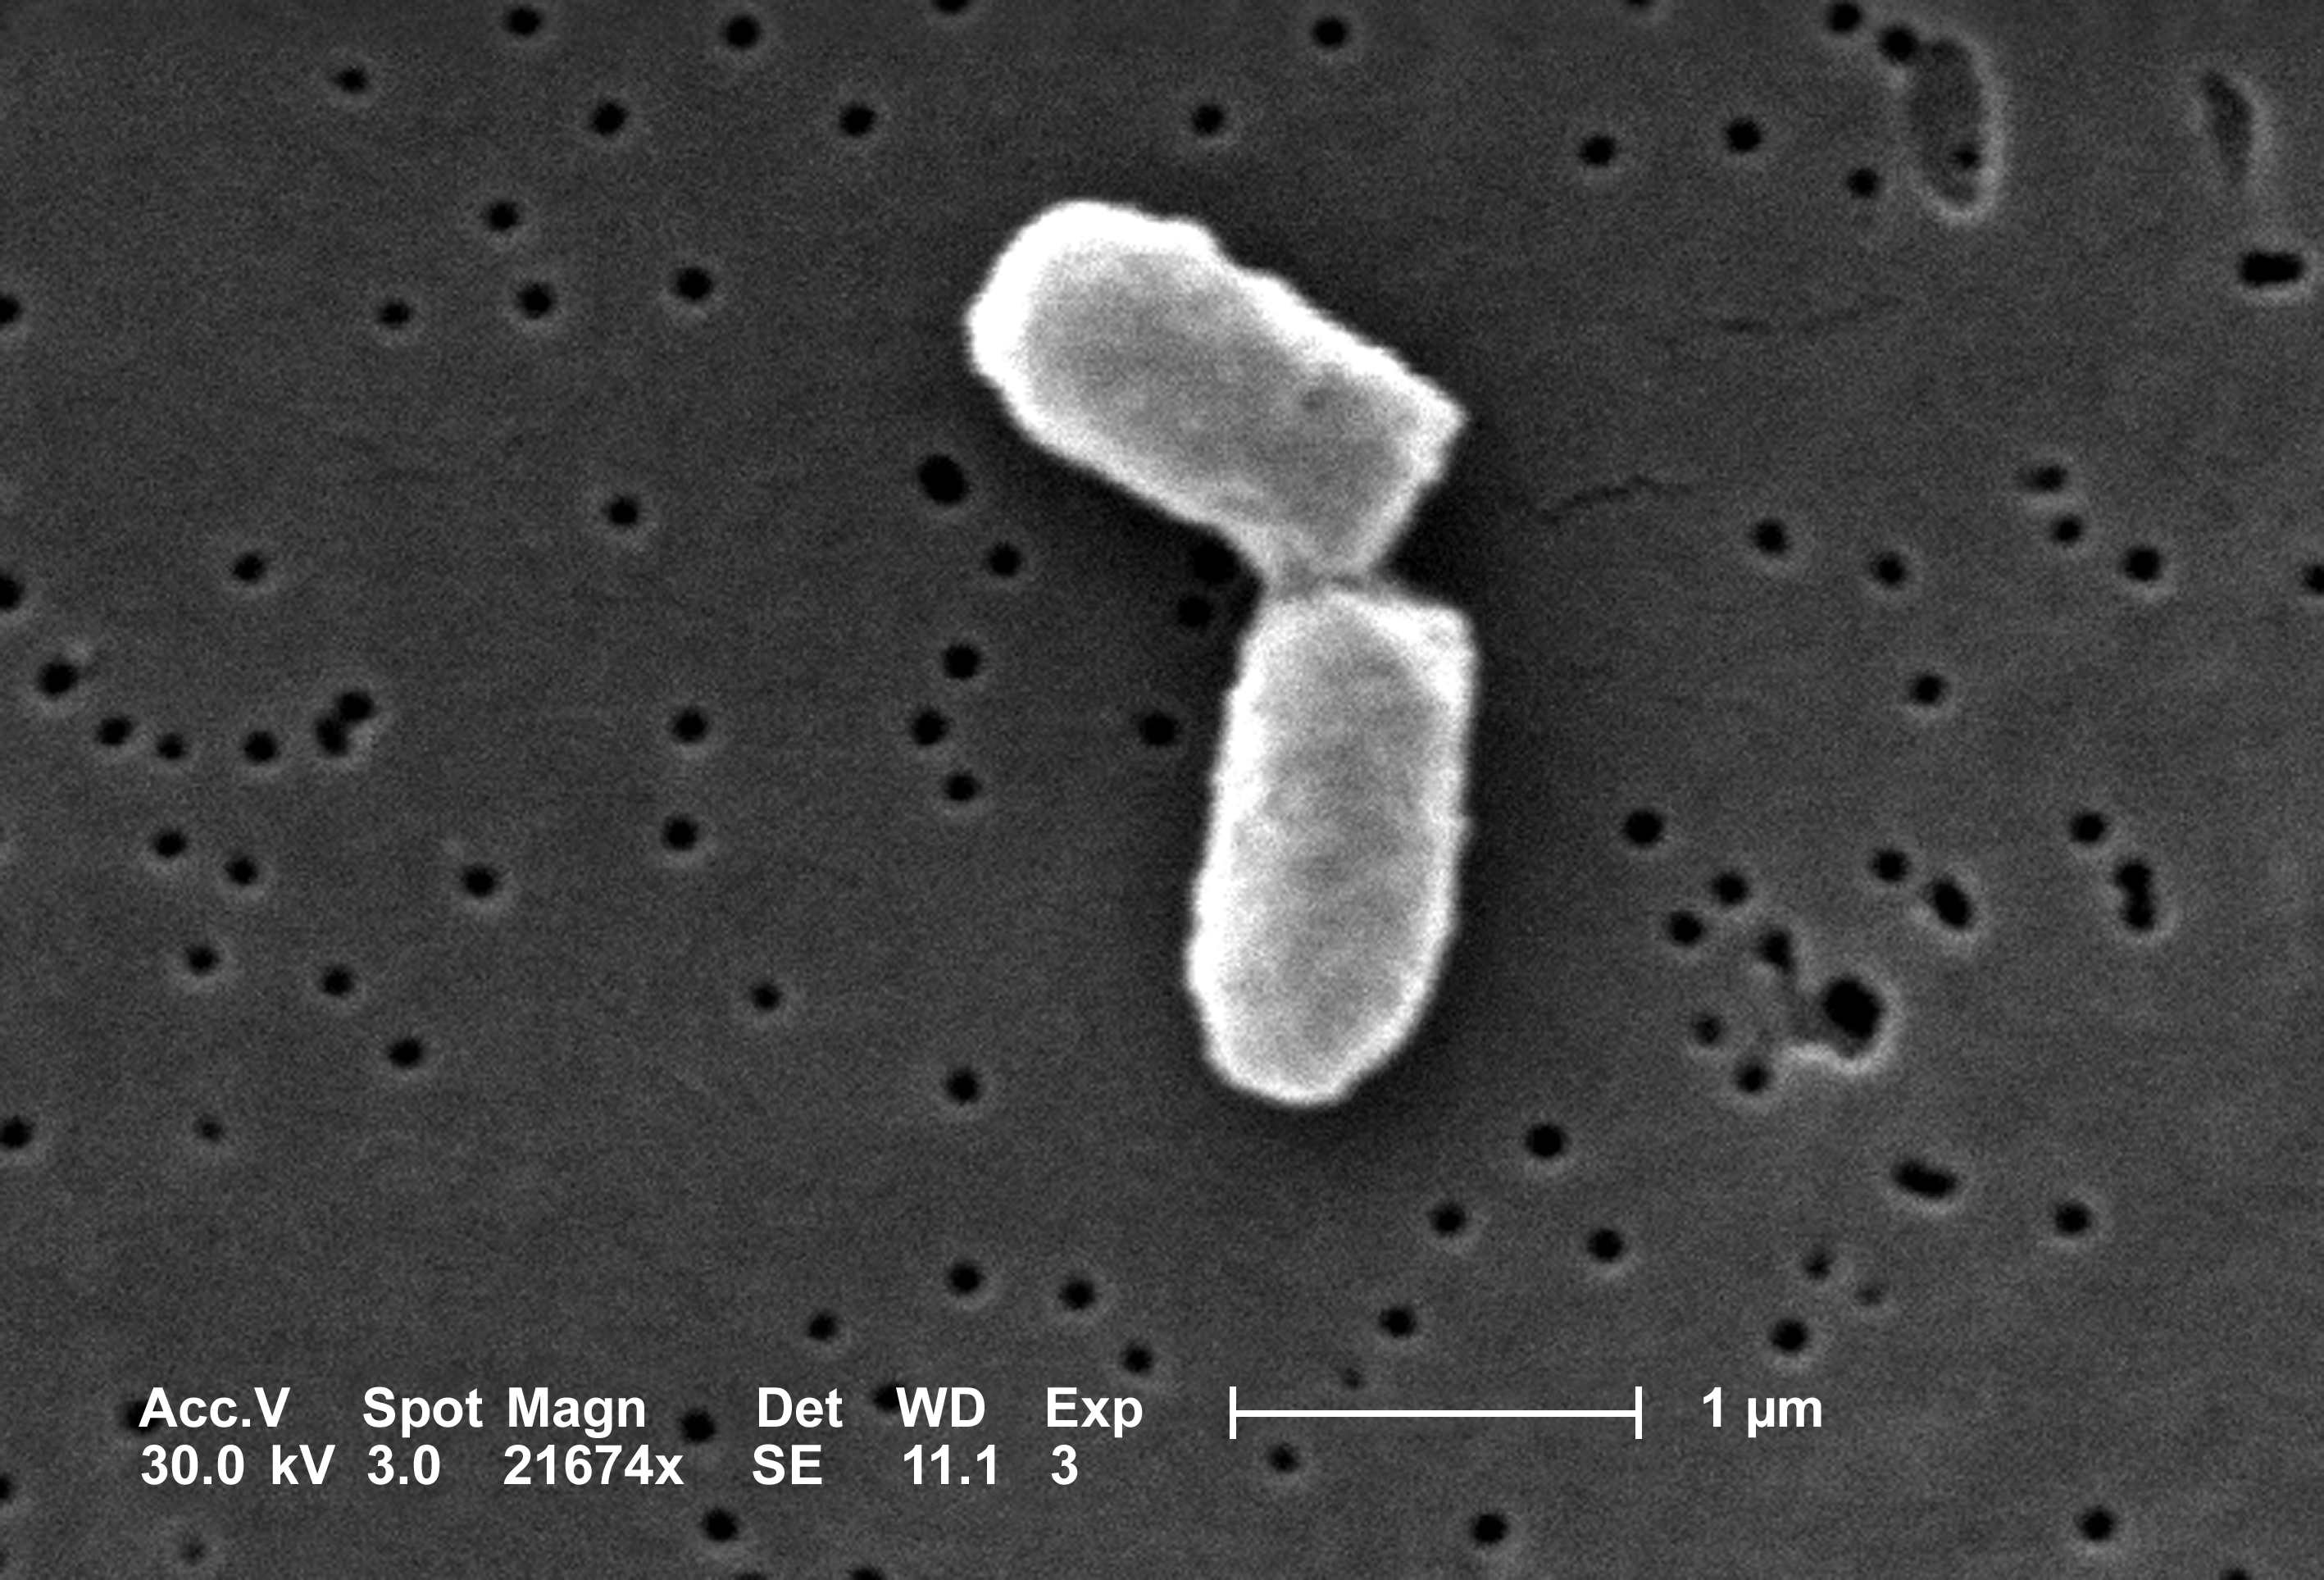
\includegraphics{ch14/Ecoli_dividing.png}
\caption{Scanning electron micrograph of a dividing \emph{Escherichia coli} bacteria; image by Evangeline Sowers, Janice Haney Carr (CDC) in public domain via Wikimedia Commons.}
\end{figure}

\hypertarget{population-with-births-and-deaths}{%
\subsection{population with births and deaths}\label{population-with-births-and-deaths}}

Suppose that a type of fish lives to reproduce only once after a period of maturation, after which the adults die. In this simple scenario, half of the population is female, a female always lays 1000 eggs, and of those, 1\% survive to maturity and reproduce. Let us set up the model for the population growth of this idealized fish population. The general idea, as before, is to relate the population size at the next time step \(N(t+1)\) to the population at the present time \(N(t)\).

Let us tabulate both the increases and the decreases in the \index{population!linear model}\index{model!population}population size. We have \(N(t)\) fish at the present time, but we know they all die after reproducing, so there is a decrease of \(N(t)\) in the population. Since half of the population is female, the number of new offspring produced by \(N(t)\) fish is \(500N(t)\). Of those, only 1\% survive to maturity (the next time step), and the other 99\% (\(495N(t)\)) die. We can add all the terms together to obtain the following difference equation:
\[ 
N(t+1) = N(t) - N(t) + 500N(t) - 495 N(t)  = 5N(t)
\]

The number 500 in the expression is the \index{population!birth rate} \emph{birth rate} of the population per individual, and the negative terms add up to the \index{population!death rate} \emph{death rate} of 496 per individual. We can re-write the equation in difference form:
\[ 
N(t+1) - N(t) = 4N(t)
\]

This expression again generates growth in the population, because the birth rate outweighs the death rate. \citep{allman_mathematical_2003}

\hypertarget{dimensions-of-birth-and-death-rates}{%
\subsection{dimensions of birth and death rates}\label{dimensions-of-birth-and-death-rates}}

As we discussed in section \ref{sec:model2} the dimensions of quantities in a model have to satisfy the rules of \index{dimensional analysis} dimensional analysis we discussed in chapter 2. In the case of population models, the birth and death rates measure the number of individuals that are born (or die) within a reproductive cycle for every individual at the present time. Their dimensions must be such that the terms in the equation all match:
\[ [N(t+1) - N(t)] = [population] = [r] [N(t)] = [r]  \times [population] \]
This implies that \(r\) is algebraically dimensionless. However, the meaning of \(r\) is the rate of change of population over one (generation) time step. \(r\) is the birth or death rate of the population \emph{per generation}, and therefore, when such rates are measured, they are reported with units of inverse time (e.g.~number of offspring per year).

\hypertarget{linear-demographic-models}{%
\subsection{linear demographic models}\label{linear-demographic-models}}

We will now write a general difference equation for any population with constant birth and death rates. This will allow us to substitute arbitrary values of the birth and death rates to model different biological situations. Suppose that a population has the birth rate of \(b\) per individual, and the death rate \(d\) per individual. Then the general model of the population size is:
\begin{equation}
 N(t+1) = (1 + b - d)N(t)
 \label{linear_pop}
\end{equation}

The general equation also allows us to check the dimensions of birth and death rates, especially as written in the incremental form: \$ N(t+1) - N(t) = (b - d)N(t)\$. The change in population rate over one reproductive cycle is given by the current population size multiplied by the difference of birth and death rates, which as we saw are algebraically dimensionless. The right hand side of the equation has the dimensions of population size, matching the difference on the left hand side. \citep{edelstein-keshet_mathematical_2005}

\hypertarget{solutions-of-linear-difference-models}{%
\section{Solutions of linear difference models}\label{solutions-of-linear-difference-models}}

\label{sec:math14}

\hypertarget{simple-linear-models}{%
\subsection{simple linear models}\label{simple-linear-models}}

Having set up the difference equation models, we would naturally like to solve them to find out how the dependent variable, such as population size, varies over time. A solution may be \index{difference equation!analytic solution} \emph{analytic}, meaning that it can be written as a formula, or \index{difference equation!numeric solution} \emph{numerical}, in which case it is generated by a computer in the form of a sequence of values of the dependent variable over a period of time. In this section, we will find some simple analytic solutions and learn to analyze the behavior of difference equations which we cannot solve exactly.\index{linear!difference equation}

\begin{definition}
\protect\hypertarget{def:diff_eqn}{}{(\#def:diff\_eqn) }A function \(N(t)\) is a \index{difference equation!solution}\emph{solution} (over some time period \(a < t < b\)) of a difference equation \(N(t+1) = f(N(t))\) if it satisfies that equation (over some time period \(a < t < b\)).
\end{definition}

\label{def:math14_sol}

For instance, let us take our first model of the static population, \(N(t+1) = N(t)\). Any constant function is a solution, for example, \(N(t) = 0\), or \(N(t) = 10\). There are actually as many solutions as there are numbers, that is, infinitely many! In order to specify exactly what happens in the model, we need to specify the size of the population at some point, usually, at the ``beginning of time'', \(t = 0\). This is called the \index{initial condition} \emph{initial condition} for the model, and for a well-behaved difference equation it is enough to determine a unique solution. For the static model, specifying the initial condition is the same as specifying the population size for all time.

Now let us look at the general model of population growth with constant birth and death rates. We saw in equation \ref{linear_pop} above that these can be written in the form \(N(t+1) = (1 + b - d) N(t)\). To simplify, let us combine the numbers into one growth parameter \(r = 1 + b - d\), and write down the general equation for population growth with constant growth rate:
\[N(t+1) =  rN(t)\]

To find the solution, consider a specific example, where we start with the initial population size \(N_0 = 1\), and the growth rate \(r=2\). The sequence of population sizes is: 1, 2, 4, 8, 16, etc. This is described by the formula \(N(t) = 2^t\).

In the general case, each time step the solution is multiplied by \(r\), so the solution has the same exponential form. The initial condition \(N_0\) is a multiplicative constant in the solution, and one can verify that when \(t=0\), the solution matches the initial value:
\begin{equation}
N(t)  = r^t N_0
\label{eq:lin_discrete_sol}
\end{equation}

I would like the reader to pause and consider this remarkable formula. No matter what the birth and death parameters are selected, this solution predicts the population size at any point in time \(t\).

In order to verify that the formula for \(N(t)\) is actually a solution in the meaning of definition \ref{def:math14_sol}, we need to check that it actually satisfies the difference equation for all \(t\), not just a few time steps. This can be done algebraically by plugging in \(N(t+1)\) into the left side of the dynamic model and \(N(t)\) into the right side and checking whether they match. For \(N(t)\) given by equation \ref{eq:lin_discrete_sol}, \(N(t+1) = r^{t+1} N_0\), and thus the dynamic model becomes:
\[r^{t+1} N_0 = r \times r^t N_0\]
Since the two sides match, \index{function!exponential}this means the solution is correct.

\hypertarget{models-with-a-constant-term}{%
\subsection{models with a constant term}\label{models-with-a-constant-term}}

Now let us consider a dynamic model that combines two different rates: a proportional rate (\(rN\)) and a constant rate which does not depend on the value of the variable \(N\). We can write such a generic model as follows:
\[ N(t+1) =  rN(t) + a \]
The right-hand-side of this equation is a linear function of \(N\), so this is a linear difference equation with a constant term. What function \(N(t)\) satisfies it? One can quickly check that that the same solution \(N(t) = r^t N_0\) does not work because of the pesky constant term \(a\):
\[ r^{t+1} N_0 \neq r \times r^t N_0 + a\]

To solve it, we need to try a different form: specifically, an exponential with an added constant. The exponential can be reasonably surmised to have base \(r\) as before, and then leave the two constants as unknown: \(N(t) = c_1 r^t + c_2\). To figure out whether this is a solution, plug it into the linear difference equation above and check whether a choice of constants can make the two sides agree:
\[  N(t+1) =  c_1 r^{t +1} + c_2 = rN(t) + a  = rc_1 r^t + rc_2+ a\]
This equation has the same term \(c_1 r^{t +1}\) on both sides, so they can be subtracted out. The remaining equation involves only \(c_2\), and its solution is \(c_2 = a/(1-r)\). Therefore, the general solution of this linear difference equation is the following expression, which is determined from the initial value by plugging \(t=0\) and solving for \(c\).
\begin{equation}
 N(t) = c r^t  + \frac{a}{1-r}
\label{eq:ch14_sol_wconst}
\end{equation}

\textbf{Example.} Take the difference equation \(N(t+1) = 0.5 N(t) + 40\) with initial value \(N(0)= 100\). The solution, according to our formula is \(N(t) = c 0.5^t + 80\). At \(N(0) = 100 = c+80\), so \(c=20\). Then the compete solution is \(N(t) = 20 \times 0.5^t + 80\). To check that this actually works, plug this solution back into the difference equation:
\[ N(t+1) = 20 \times 0.5^{t+1} + 80 = 0.5 \times (20 \times 0.5^t + 80) + 40 =  20 \times 0.5^{t+1} + 80\]
The equation is satisfied and therefore the solution is correct.

\hypertarget{population-growth-and-decline}{%
\subsection{population growth and decline}\label{population-growth-and-decline}}

\label{sec:bio14}

The parameter \(r\) can assume different values, depending on the birth and death rates. If the birth rate is greater than the death rate, \(r > 1\), and if it is the other way around, \(r < 1\). Note that for a realistic biological population, the death rate is limited by the number of individuals present in the population. The maximum number of individuals at any time is \(N(t)+bN(t)\), so this means that \(d \leq b +1\). Therefore, for a biological population, \(r \geq 0\).

\begin{Shaded}
\begin{Highlighting}[]
\NormalTok{x \textless{}{-}}\StringTok{ }\DecValTok{0}\OperatorTok{:}\DecValTok{6}
\NormalTok{y0 \textless{}{-}}\StringTok{ }\DecValTok{5}
\KeywordTok{plot}\NormalTok{(x, y0 }\OperatorTok{*}\StringTok{ }\DecValTok{2}\OperatorTok{\^{}}\NormalTok{x, }\DataTypeTok{t =} \StringTok{"b"}\NormalTok{, }\DataTypeTok{lwd =} \DecValTok{3}\NormalTok{, }\DataTypeTok{cex.axis =} \FloatTok{1.5}\NormalTok{, }
    \DataTypeTok{cex.lab =} \FloatTok{1.5}\NormalTok{, }\DataTypeTok{xlab =} \StringTok{"time"}\NormalTok{, }\DataTypeTok{ylab =} \StringTok{"population"}\NormalTok{)}
\NormalTok{y0 \textless{}{-}}\StringTok{ }\DecValTok{1}
\KeywordTok{lines}\NormalTok{(x, y0 }\OperatorTok{*}\StringTok{ }\DecValTok{2}\OperatorTok{\^{}}\NormalTok{x, }\DataTypeTok{t =} \StringTok{"b"}\NormalTok{, }\DataTypeTok{lwd =} \DecValTok{3}\NormalTok{, }\DataTypeTok{col =} \DecValTok{2}\NormalTok{)}
\NormalTok{leg.txt \textless{}{-}}\StringTok{ }\KeywordTok{c}\NormalTok{(}\StringTok{"N(0)=5"}\NormalTok{, }\StringTok{"N(0)=1"}\NormalTok{)}
\KeywordTok{legend}\NormalTok{(}\StringTok{"topleft"}\NormalTok{, leg.txt, }\DataTypeTok{cex =} \FloatTok{1.5}\NormalTok{, }\DataTypeTok{col =} \KeywordTok{c}\NormalTok{(}\DecValTok{1}\NormalTok{, }\DecValTok{2}\NormalTok{), }
    \DataTypeTok{pch =} \DecValTok{1}\NormalTok{, }\DataTypeTok{lty =} \DecValTok{1}\NormalTok{, }\DataTypeTok{lwd =} \DecValTok{3}\NormalTok{)}
\NormalTok{y0 \textless{}{-}}\StringTok{ }\DecValTok{1000}
\KeywordTok{plot}\NormalTok{(x, y0 }\OperatorTok{*}\StringTok{ }\FloatTok{0.5}\OperatorTok{\^{}}\NormalTok{x, }\DataTypeTok{t =} \StringTok{"b"}\NormalTok{, }\DataTypeTok{lwd =} \DecValTok{3}\NormalTok{, }\DataTypeTok{cex.axis =} \FloatTok{1.5}\NormalTok{, }
    \DataTypeTok{cex.lab =} \FloatTok{1.5}\NormalTok{, }\DataTypeTok{xlab =} \StringTok{"time"}\NormalTok{, }\DataTypeTok{ylab =} \StringTok{"population"}\NormalTok{)}
\NormalTok{y0 \textless{}{-}}\StringTok{ }\DecValTok{500}
\KeywordTok{lines}\NormalTok{(x, y0 }\OperatorTok{*}\StringTok{ }\FloatTok{0.5}\OperatorTok{\^{}}\NormalTok{x, }\DataTypeTok{t =} \StringTok{"b"}\NormalTok{, }\DataTypeTok{lwd =} \DecValTok{3}\NormalTok{, }\DataTypeTok{col =} \DecValTok{2}\NormalTok{)}
\NormalTok{leg.txt \textless{}{-}}\StringTok{ }\KeywordTok{c}\NormalTok{(}\StringTok{"N(0)=1000"}\NormalTok{, }\StringTok{"N(0)=500"}\NormalTok{)}
\KeywordTok{legend}\NormalTok{(}\StringTok{"topright"}\NormalTok{, leg.txt, }\DataTypeTok{cex =} \FloatTok{1.5}\NormalTok{, }\DataTypeTok{col =} \KeywordTok{c}\NormalTok{(}\DecValTok{1}\NormalTok{, }\DecValTok{2}\NormalTok{), }
    \DataTypeTok{pch =} \DecValTok{1}\NormalTok{, }\DataTypeTok{lty =} \DecValTok{1}\NormalTok{, }\DataTypeTok{lwd =} \DecValTok{3}\NormalTok{)}
\end{Highlighting}
\end{Shaded}

\begin{figure}

{\centering 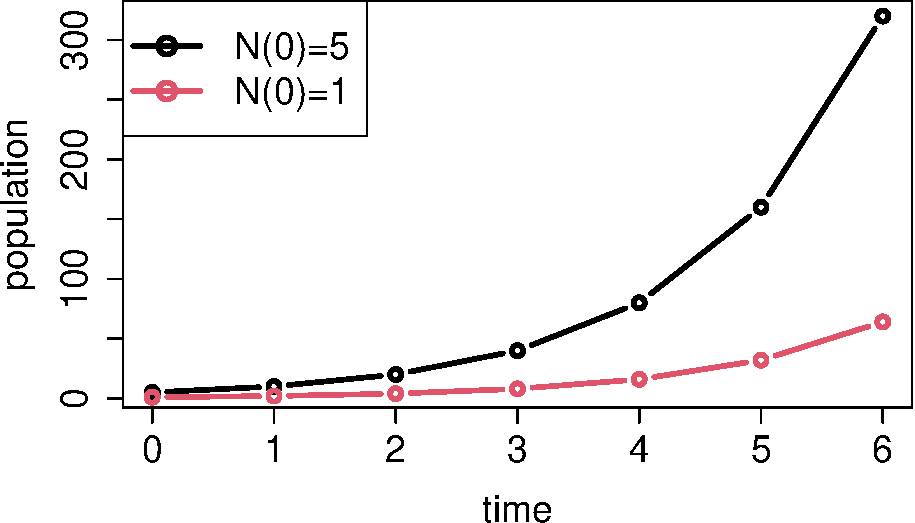
\includegraphics[width=0.5\linewidth]{QuantLife_files/figure-latex/ch14-sol-1} 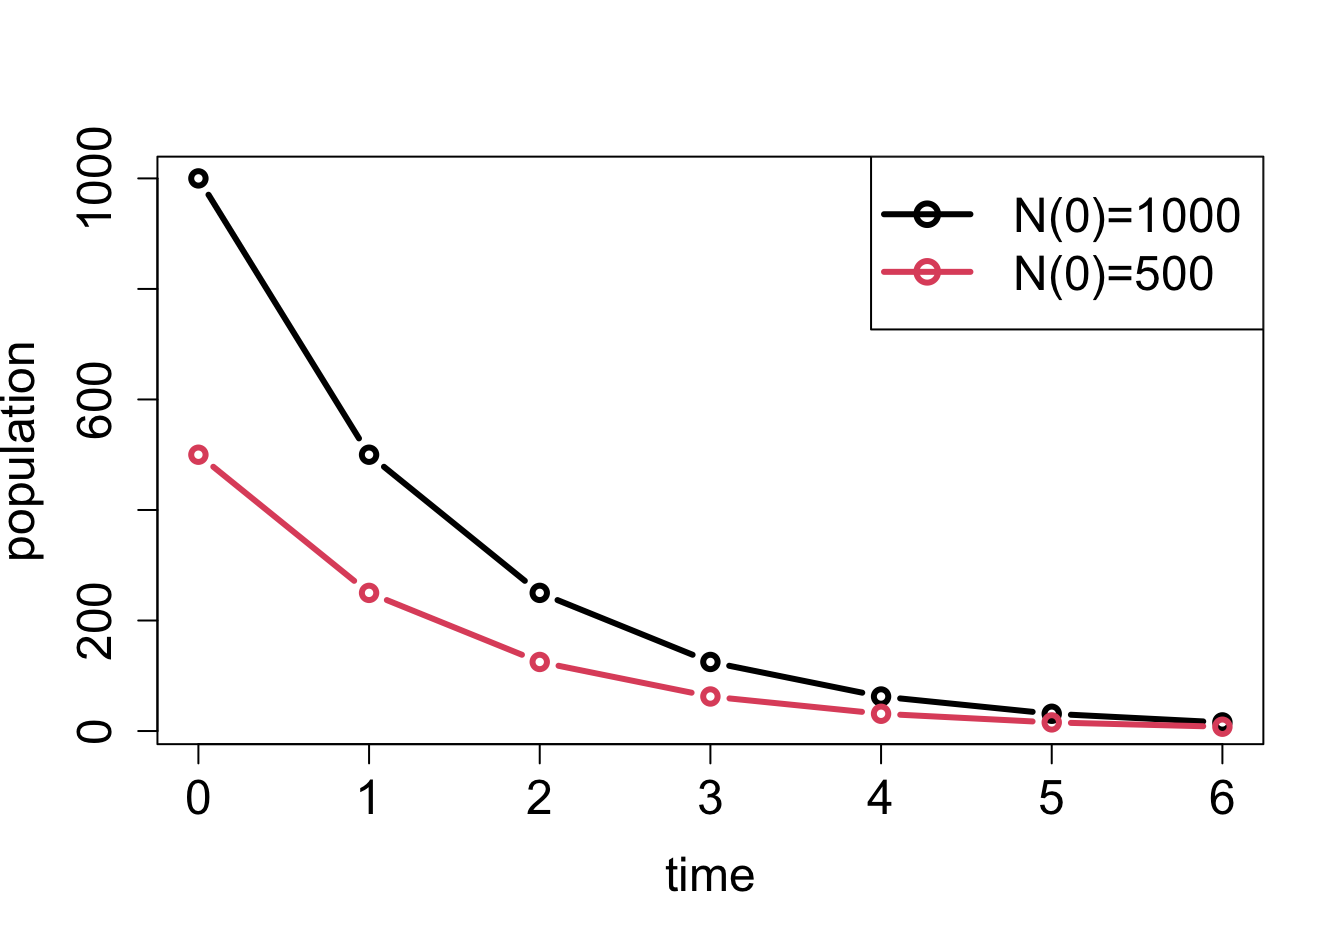
\includegraphics[width=0.5\linewidth]{QuantLife_files/figure-latex/ch14-sol-2} 

}

\caption{Plots of solutions of linear difference equations: a) $N(t+1) = 2N(t)$ with different initial values; b) $N(t+1) = 0.5N(t)$ with different initial values}\label{fig:ch14-sol}
\end{figure}

The solutions in formula \ref{eq:lin_discrete_sol} and \ref{eq:ch14_sol_wconst} are exponential functions, which as we saw in section \ref{sec:math2} have a limited menu of behaviors, depending on the value of \(r\). If \(r > 1\), multiplication by \(r\) increases the size of the population, so the solution \(N(t)\) will grow. If \(r < 1\), multiplication by \(r\) decreases the size of the population, so the solution \(N(t)\) will decay (see figure \ref{fig:ch14_solutions}). Finally, if \(r=1\), multiplication by \(r\) leaves the population size unchanged, like in the pile of rocks model. Here is the complete classification of the behavior of population models with constant birth and death rates (assuming \(r>0\)):

\begin{itemize}
\tightlist
\item
  \(r > 1\): \(N(t)\) grows without bound
\item
  \(r < 1\): \(N(t)\) decays to the constant \(a/(1-r)\)
\item
  \(r = 1\): \(N(t)\) remains constant
\end{itemize}

As we see, there are only two options for solution of linear difference equations: ever-faster growth or decay to zero or another constant value. The exponential growth of populations is also known as \index{model!Malthusian growth} \emph{Malthusian} after the early population modeler Thomas Malthus. He used a simple population model with constant growth rate to predict demographic disaster due to the exponentially increasing population outstripping the growth in food production. In fact, human population has not been growing with a constant birth rate, and food production has (so far) kept up pace with population size, illustrating yet again that mathematical models are only as good as the assumptions that underlie them.

\hypertarget{exercises-12}{%
\subsection{Exercises}\label{exercises-12}}

For the following scenarios for a population: 1) Construct a dynamic model by writing down a difference equation both in the updating function form (\(N(t+1) = f(N(t))\)) and the increment form (\(N(t+1) - N(t) = g(N(t))\)) and specify the time step; 2) find the solution of the linear difference equation with a generic initial value and check that it satisfies the difference equation by plugging the solution into your equation (in either form); 3) plug in the given initial value and predict the future.

\begin{enumerate}
\def\labelenumi{\arabic{enumi}.}
\item
  Zombies have appeared in Chicago. Every day, each zombie produces 3 new zombies. Suppose that initially there is only one zombie, how many zombies will there be in 7 days?
\item
  Suppose hunters kill 50 deer in a national forest every hunting season, while the deer by themselves have equal birth and death rates. If there are initially 500 deer in the forest, predict how many there will be in 5 years.
\item
  The number of infected people in a population grows by 8\% per day and those who become infected remain infected. If initially there are 8 infected, how many individuals will be infected in 45 days?
\item
  Suppose bacteria in a population divide in 2 every hour and 90\% of the current population dies after reproduction, not including the new offspring. If the population initially has 10 million bacteria, predict how many there will be in 12 hours.
\item
  In a rabbit population, each pair produces 2.2 offspring every year (i.e.~1.1 per capita) and the adults have a 0.9 annual death rate after reproduction (and assume the whole population is paired up into mating pairs.) If initially there are 55 rabbits, predict how many there will be in 5 years.
\item
  Consider the same rabbit population, but now a python that lives nearby eats exactly 1 rabbit a month. If initially there are 55 rabbits, how many do you predict will be in 10 years?
\item
  10 fish are added to an aquarium every month, while 80\% of those present survive every month and there is no reproduction. If initially there are 10 fish in the aquarium, predict how many there will be in 2 years.
\item
  A Mardi Gras parade marches down the street, and every block 50 new revelers join the parade, while 20\% of parade leaves for various reasons. Suppose the parade starts with 12 people, predict how many there will be after 30 blocks.
\item
  Twenty flies fly into a house every day, and half of the flies in the house at beginning of each day find their way out (no births or deaths happen in the house.) If there are 10 files in the house initially, how many will there be in 12 days?
\item
  Every day someone eats 10 pieces of candy from a bowl, while someone else adds half as many pieces as are currently in the bowl (before 10 pieces are removed.) If there are currently 20 pieces of candy in the bowl, how many will there be in 7 days?
\end{enumerate}

\hypertarget{numerical-solutions-in-r}{%
\section{Numerical solutions in R}\label{numerical-solutions-in-r}}

\label{sec:comp14}

\hypertarget{for-loops}{%
\subsection{for loops}\label{for-loops}}

Often times one has to write a script to perform the same (or similar) task many times. Like all programming languages, R has commands that call for repetition of the same commands multiple times. These structures are called \emph{loops}. In this section you will learn about the \index{R programming!for loop} \emph{for loop}, which looks like this:

\begin{Shaded}
\begin{Highlighting}[]
\ControlFlowTok{for}\NormalTok{ (i }\ControlFlowTok{in} \DecValTok{1}\OperatorTok{:}\DecValTok{10}\NormalTok{) \{}
\NormalTok{    body of the loop}
\NormalTok{\}}
\end{Highlighting}
\end{Shaded}

For example, the following script will print out ``Hello!'' ten times like this:

\begin{Shaded}
\begin{Highlighting}[]
\ControlFlowTok{for}\NormalTok{ (i }\ControlFlowTok{in} \DecValTok{1}\OperatorTok{:}\DecValTok{10}\NormalTok{) \{}
    \KeywordTok{print}\NormalTok{(}\StringTok{"Hello!"}\NormalTok{)}
\NormalTok{\}}
\end{Highlighting}
\end{Shaded}

\begin{verbatim}
## [1] "Hello!"
## [1] "Hello!"
## [1] "Hello!"
## [1] "Hello!"
## [1] "Hello!"
## [1] "Hello!"
## [1] "Hello!"
## [1] "Hello!"
## [1] "Hello!"
## [1] "Hello!"
\end{verbatim}

The for loop starts with the keyword \texttt{for}, then has the expression in parentheses (i in 1:10). \texttt{i} is called the \emph{loop variable}, \texttt{in} is another keyword, and \texttt{1:10} is a \emph{loop vector}. After the first line there is a curly bracket \{ and everything that follows until the closing bracket \} is the \emph{loop body}. The loop body is executed as many times as there are elements in the loop vector (in this example, 10 times) and the only thing that changes is the values of the loop variable i, which starts with the first element of the vector (1) and goes until it reaches the last element (10) and then stops:

\begin{Shaded}
\begin{Highlighting}[]
\ControlFlowTok{for}\NormalTok{ (i }\ControlFlowTok{in} \DecValTok{1}\OperatorTok{:}\DecValTok{10}\NormalTok{) \{}
  \KeywordTok{print}\NormalTok{(}\KeywordTok{paste}\NormalTok{(}\StringTok{"Iteration number"}\NormalTok{, i))}
\NormalTok{\}}
\end{Highlighting}
\end{Shaded}

\begin{verbatim}
## [1] "Iteration number 1"
## [1] "Iteration number 2"
## [1] "Iteration number 3"
## [1] "Iteration number 4"
## [1] "Iteration number 5"
## [1] "Iteration number 6"
## [1] "Iteration number 7"
## [1] "Iteration number 8"
## [1] "Iteration number 9"
## [1] "Iteration number 10"
\end{verbatim}

It can be used to do repetitive calculations, for example, adding up all the integers in an array (of course the built-in function \texttt{sum()} will do it too):

\begin{Shaded}
\begin{Highlighting}[]
\CommentTok{\# add up the integers from 1 to 10 and print out the total}
\NormalTok{total\textless{}{-}}\DecValTok{0}
\ControlFlowTok{for}\NormalTok{ (i }\ControlFlowTok{in} \DecValTok{1}\OperatorTok{:}\DecValTok{10}\NormalTok{) \{}
\NormalTok{  total\textless{}{-}total}\OperatorTok{+}\NormalTok{i}
\NormalTok{\}}
\KeywordTok{print}\NormalTok{(total)}
\end{Highlighting}
\end{Shaded}

\begin{verbatim}
## [1] 55
\end{verbatim}

\hypertarget{using-vectors-with-loops}{%
\subsection{using vectors with loops}\label{using-vectors-with-loops}}

It is especially useful to use loops to assign vector variables one element at a time. The loop variable (e.g.~\texttt{i}) is usually used for \emph{indexing} the vector variable. There are several necessary features of using vectors in for loops, so let us take an example script and break them down in this example of calculating a vector of the sum of integers from 1 up to the current number:

\begin{enumerate}
\def\labelenumi{\arabic{enumi}.}
\tightlist
\item
  \emph{Pre-allocate} the vector variable: create a vector of the correct length prior to the loop by filling it with a placeholder value, e.g.~0 or NA (not a value).
\end{enumerate}

\begin{Shaded}
\begin{Highlighting}[]
\NormalTok{max \textless{}{-}}\StringTok{ }\DecValTok{10}
\NormalTok{total\_vec \textless{}{-}}\StringTok{ }\KeywordTok{rep}\NormalTok{(}\DecValTok{0}\NormalTok{, max }\OperatorTok{+}\StringTok{ }\DecValTok{1}\NormalTok{)  }\CommentTok{\# pre{-}allocate the vector}
\end{Highlighting}
\end{Shaded}

\begin{enumerate}
\def\labelenumi{\arabic{enumi}.}
\setcounter{enumi}{1}
\tightlist
\item
  Only put in the loop what has to be repeated (e.g.~don't put the pre-allocation inside the loop);
\end{enumerate}

\begin{Shaded}
\begin{Highlighting}[]
\ControlFlowTok{for}\NormalTok{ (i }\ControlFlowTok{in} \DecValTok{1}\OperatorTok{:}\NormalTok{max) \{ }\CommentTok{\# iterate for i from 1 to max}
\NormalTok{  total\_vec[i}\OperatorTok{+}\DecValTok{1}\NormalTok{] \textless{}{-}}\StringTok{ }\NormalTok{total\_vec[i] }\OperatorTok{+}\StringTok{ }\NormalTok{i }\CommentTok{\# assign to the next value of total\_vec the sum of i and the current value of total\_vec}
\NormalTok{\}}
\end{Highlighting}
\end{Shaded}

\begin{enumerate}
\def\labelenumi{\arabic{enumi}.}
\setcounter{enumi}{2}
\tightlist
\item
  Be careful with indexing inside for loops - this means paying careful attention to the lowest and the highest index that you're using inside the loop. For example, if your loop vector goes from 1 to max (as above), the total number of elements in your vector will be max+1, because we assigned the element with index i+1 in the loop:
\end{enumerate}

\begin{Shaded}
\begin{Highlighting}[]
\KeywordTok{print}\NormalTok{(}\KeywordTok{length}\NormalTok{(total\_vec)) }\CommentTok{\# print the number of elements of total\_vec}
\end{Highlighting}
\end{Shaded}

\begin{verbatim}
## [1] 11
\end{verbatim}

\begin{Shaded}
\begin{Highlighting}[]
\KeywordTok{print}\NormalTok{(total\_vec)}
\end{Highlighting}
\end{Shaded}

\begin{verbatim}
##  [1]  0  1  3  6 10 15 21 28 36 45 55
\end{verbatim}

Here is an example of a loop calculating the famous Fibonacci sequence, where the next value is defined to be the sum of two previous values in the sequence, and the plotting the resulting sequence, together with an exponential function that approximates it.

\begin{Shaded}
\begin{Highlighting}[]
\NormalTok{num\_steps \textless{}{-}}\StringTok{ }\DecValTok{20} \CommentTok{\# number of steps}
\NormalTok{fib \textless{}{-}}\StringTok{ }\KeywordTok{rep}\NormalTok{(}\DecValTok{1}\NormalTok{, num\_steps }\OperatorTok{+}\StringTok{ }\DecValTok{2}\NormalTok{) }\CommentTok{\# pre{-}allocate vector with correct number of elements with all 1s}
\ControlFlowTok{for}\NormalTok{ (i }\ControlFlowTok{in} \DecValTok{1}\OperatorTok{:}\NormalTok{num\_steps) \{}
\NormalTok{  fib[i}\OperatorTok{+}\DecValTok{2}\NormalTok{] \textless{}{-}}\StringTok{ }\NormalTok{fib[i}\OperatorTok{+}\DecValTok{1}\NormalTok{] }\OperatorTok{+}\StringTok{ }\NormalTok{fib[i] }\CommentTok{\# add elements i and i+1 and assign it to element i+2}
\NormalTok{\}}
\NormalTok{time \textless{}{-}}\StringTok{ }\DecValTok{0}\OperatorTok{:}\NormalTok{(num\_steps}\OperatorTok{+}\DecValTok{1}\NormalTok{) }\CommentTok{\# define a "time" vector as the independent variable}
\KeywordTok{plot}\NormalTok{ (time, fib, }\DataTypeTok{lwd =} \DecValTok{3}\NormalTok{, }\DataTypeTok{xlab =} \StringTok{\textquotesingle{}time steps\textquotesingle{}}\NormalTok{, }\DataTypeTok{ylab =} \StringTok{"Fibonacci"}\NormalTok{)}
\CommentTok{\# an exponential function wiht the Golden ratio base}
\NormalTok{phi \textless{}{-}}\StringTok{ }\NormalTok{(}\DecValTok{1}\OperatorTok{+}\KeywordTok{sqrt}\NormalTok{(}\DecValTok{5}\NormalTok{))}\OperatorTok{/}\DecValTok{2} \CommentTok{\# golden ratio}
\NormalTok{sol \textless{}{-}}\StringTok{ }\FloatTok{0.75}\OperatorTok{*}\NormalTok{phi}\OperatorTok{\^{}}\NormalTok{time }\CommentTok{\# calculate the exponential function vector (no loop required)}
\KeywordTok{lines}\NormalTok{(time, sol, }\DataTypeTok{col=}\StringTok{\textquotesingle{}red\textquotesingle{}}\NormalTok{, }\DataTypeTok{lwd =} \DecValTok{3}\NormalTok{) }\CommentTok{\# overlay the exponential function plot}
\KeywordTok{legend}\NormalTok{(}\StringTok{"topleft"}\NormalTok{, }\CommentTok{\# legend placement}
       \KeywordTok{c}\NormalTok{(}\StringTok{"Fibonacci"}\NormalTok{, }\StringTok{"exponential"}\NormalTok{), }\CommentTok{\# vector containing labels for the legend}
       \DataTypeTok{col=}\DecValTok{1}\OperatorTok{:}\DecValTok{2}\NormalTok{, }\CommentTok{\# vector containing color codes (1 is black, 2 is red)}
       \DataTypeTok{lty=}\KeywordTok{c}\NormalTok{(}\DecValTok{0}\NormalTok{,}\DecValTok{1}\NormalTok{), }\CommentTok{\# vector specifying line types (0 is none, 1 is regular line)}
       \DataTypeTok{pch=}\KeywordTok{c}\NormalTok{(}\DecValTok{1}\NormalTok{,}\OtherTok{NA}\NormalTok{), }\CommentTok{\# vector specifying types of point markers (1 is cicle, NA is none)}
       \DataTypeTok{lwd=}\DecValTok{3}\NormalTok{) }
\end{Highlighting}
\end{Shaded}

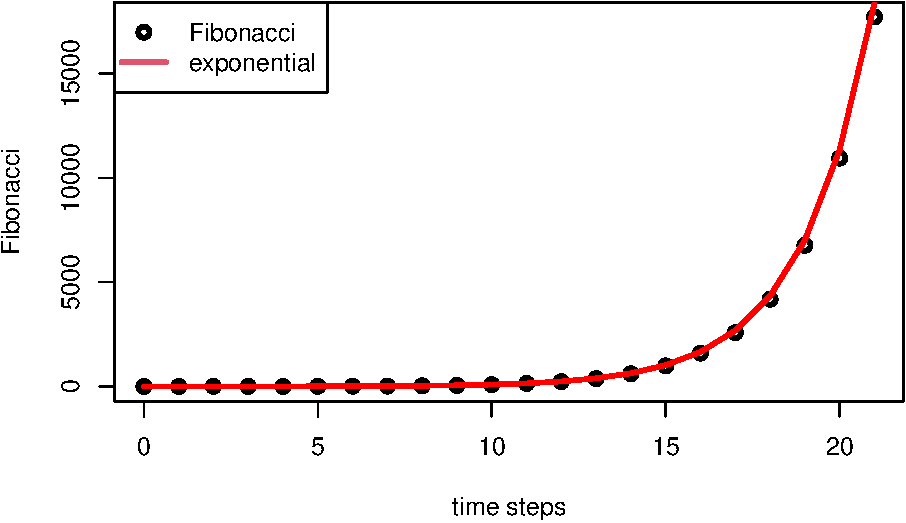
\includegraphics{QuantLife_files/figure-latex/unnamed-chunk-96-1.pdf}

\hypertarget{exercises-13}{%
\subsection{Exercises:}\label{exercises-13}}

\begin{enumerate}
\def\labelenumi{\arabic{enumi}.}
\item
  Assign the value 5 to a variable and multiply it by 1.03, replacing the old value of the variable. The new value should be 5.15.
\item
  Write a script to take a number and multiply it by 1.03 one hundred times using a for loop (see section 4.4.2) Starting with the initial value 5, the script should return the value 96.093.
\item
  Preallocate a vector of values to be all zeros, assign the first element to 5, and then use a for loop to calculate 100 values by multiplying the previous one by 1.03 and assigning them to sequential elements of the vector, then plot that vector. You should see an exponentially growing curve, with the last element (101st) equal to 96.093.
\item
  Fix the indexing error in the script below for calculating a vector of factorials. Each element of the vector \texttt{factorial\_vec{[}i{]}} should be equal to \(i!= 1*2*3...*i\), so for example \texttt{factorial\_vec{[}2{]}} should be 2 and \texttt{factorial\_vec{[}3{]}} should be 6.
\end{enumerate}

\begin{Shaded}
\begin{Highlighting}[]
\CommentTok{\# multiply integers from 1 to 10 and assign the factorials to the vector }
\NormalTok{max.num \textless{}{-}}\StringTok{ }\DecValTok{10}
\NormalTok{factorial\_vec \textless{}{-}}\StringTok{ }\KeywordTok{rep}\NormalTok{(}\DecValTok{1}\NormalTok{,max.num)}
\ControlFlowTok{for}\NormalTok{ (i }\ControlFlowTok{in} \DecValTok{1}\OperatorTok{:}\NormalTok{max.num) \{}
\NormalTok{  factorial\_vec[i}\OperatorTok{+}\DecValTok{1}\NormalTok{]\textless{}{-}factorial\_vec[i]}\OperatorTok{*}\NormalTok{i}
\NormalTok{\}}
\KeywordTok{print}\NormalTok{(factorial\_vec)}
\end{Highlighting}
\end{Shaded}

\hypertarget{r-assignment-4}{%
\section{R Assignment}\label{r-assignment-4}}

In this part you will calculate numeric solutions of difference equations. Use the code from the last of the exercises above to write a script to iteratively update the variable for a specified number of steps and store it as a vector, and plot it as function of time. Hint: your code will be nearly identical for all the tasks, so once you get the first script to work properly, copy and paste it and modify the line in the for loop that calculates the next values. Please use descriptive names for variables and label your axes!

For each of the following questions, do these tasks:

\begin{enumerate}
\def\labelenumi{\arabic{enumi}.}
\item
  write down the difference equation for the model;
\item
  calculate the numerical solution for the model with the given initial values and for the specified time period;
\item
  plot the solution over time (create vector for time!);
\item
  describe how the solution behaves in the long term and whether it depends on the initial value (try different initial values!)
\item
  The number of infected people in a population grows by 8\% per day and those who become infected remain infected. If initially there are 8 infected, how many individuals will be infected in 45 days? ANSWER: about 255
\end{enumerate}

\begin{Shaded}
\begin{Highlighting}[]
\CommentTok{\# YOUR CODE HERE}
\end{Highlighting}
\end{Shaded}

YOUR ANSWERS GO HERE

\begin{enumerate}
\def\labelenumi{\arabic{enumi}.}
\setcounter{enumi}{1}
\tightlist
\item
  Suppose bacteria in a population divide in 2 every hour and 90\% of the current population dies after reproduction, not including the new offspring. If the population initially has 10 million bacteria, predict how many there will be in 24 hours. ANSWER: about 98497327
\end{enumerate}

\begin{Shaded}
\begin{Highlighting}[]
\CommentTok{\# YOUR CODE HERE}
\end{Highlighting}
\end{Shaded}

YOUR ANSWERS GO HERE

\begin{enumerate}
\def\labelenumi{\arabic{enumi}.}
\setcounter{enumi}{2}
\tightlist
\item
  In a rabbit population, each pair produces 2.2 offspring every year (i.e.~1.1 per capita) and the adults have a 0.9 annual death rate after reproduction (and assume the whole population is paired up into mating pairs.) If initially there are 60 rabbits, predict how many there will be in 25 years. ANSWER: about 5724
\end{enumerate}

\begin{Shaded}
\begin{Highlighting}[]
\CommentTok{\# YOUR CODE HERE}
\end{Highlighting}
\end{Shaded}

YOUR ANSWERS GO HERE

\begin{enumerate}
\def\labelenumi{\arabic{enumi}.}
\setcounter{enumi}{3}
\tightlist
\item
  Consider the same rabbit population, but now a python that lives nearby eats exactly 1 rabbit \emph{per month}. If initially there are 60 rabbits, predict how many there will be in 25 years. ANSWER: 60
\end{enumerate}

\begin{Shaded}
\begin{Highlighting}[]
\CommentTok{\# YOUR CODE HERE}
\end{Highlighting}
\end{Shaded}

YOUR ANSWERS GO HERE

\begin{enumerate}
\def\labelenumi{\arabic{enumi}.}
\setcounter{enumi}{4}
\tightlist
\item
  10 fish are added to an aquarium every month, while 80\% of those present survive every month and there is no reproduction. If initially there are 10 fish in the aquarium, predict how many there will be in a year. ANSWER: about 47
\end{enumerate}

\begin{Shaded}
\begin{Highlighting}[]
\CommentTok{\# YOUR CODE HERE}
\end{Highlighting}
\end{Shaded}

YOUR ANSWERS GO HERE

\hypertarget{linear-ordinary-differential-equations}{%
\chapter{Linear ordinary differential equations}\label{linear-ordinary-differential-equations}}

\begin{quote}
He felt a restless, vague ambition\\
A craving for a change of air\\
(A most unfortunate condition,\\
A cross not many choose to bear.)\\
-- Alexander Pushkin, \emph{Eugene Onegin}
\end{quote}

In the last chapter we considered discrete time models, in which time is counted in integers. This worked well to describe processes that happen in periodic cycles, like cell division or heart pumping. Many biological systems do not work this way. Change can happen continuously, that is, at any moment in time. For instance, the concentration of a biological molecule in the cell changes gradually, as does the voltage across the cell membrane in a neuron.

There are at least two good reasons to use differential equations for many applications. First, they are often more realistic than discrete time models, because some events happen very frequently and non-periodically. The second reason is mathematical: it turns out that dynamical systems with continuous time, described by differential equations, are better behaved than difference equations. This has to do with the essential ``jumpiness'' of difference equations. Even for simple nonlinear equations, the value of the variable after one time step can be far removed from its last value. This can lead to highly complicated solutions, as we saw in some of the numerical solutions in the last chapter. That kind of erratic behavior is impossible in one-variable differential equations (provided they have continuous defining functions.) In this chapter you will learn to do the following:

\%The models for continuously changing variables require their own set of mathematical tools. Instead of difference equations, we are going to see our first differential equations, which use derivatives to describe how a variable changes with time. There is a tremendous amount of knowledge accumulated by mathematicians, physicists and engineers for analyzing and solving differential equations. There are many classes of differential equations for which it is possible to find analytic solutions, often in the form of so-called special functions. Differential equations courses for physicists and engineers are typically focused on learning about the variety of existing tools for solving a few types of differential equations. For the purposes of biological modeling, knowing how to solve a limited number of differential equations is of limited usefulness. We will instead focus on learning how to analyze the behavior of differential equations in general, without having to solve them on paper.

\begin{itemize}
\item
  build differential equations based on stated assumptions
\item
  find analytic solutions of linear differential equations
\item
  compute numerical solutions of differential equations using the Forward Euler method
\end{itemize}

\hypertarget{building-differential-equations}{%
\section{Building differential equations}\label{building-differential-equations}}

\label{sec:model15}

\hypertarget{from-discrete-time-to-continuous}{%
\subsection{from discrete time to continuous}\label{from-discrete-time-to-continuous}}

In this chapter we investigate \index{model!continuous time} \emph{continuous time dynamical systems}, for which it does not make sense to break time up into equal intervals. Instead of equations describing the increments in the dependent variable from one time step to the next, we will see equations with the instantaneous rate of the change (derivative) of the variable. Let us see the connection between the discrete and continuous dynamic models by reducing the step size of the bacteria-division population model.

First, suppose that instead of dividing every hour, \index{population!bacteria}\index{bacteria!division}the population of bacteria divide every half-hour, but only half of the population does. That half is chosen randomly, so we don't have to keep track of whether each bacterium divided the last time around or not. Therefore, each half-hour exactly half of the population is added to the current population:
\[ N(t+0.5) = N(t) + 0.5N(t) = 1.5N(t)\]
The solution for this model can be figured out from the linear difference equation solution we derived in section \ref{sec:math14} Every half-hour, the population is multiplied by 1.5, so we can write:
\[ N(t) = 1.5^{2t} N(0) = (1.5^2)^t N(0)\]
Compare this solution with the one for the every-hour model, \(N(t) = 2^t N(0)\) by plugging in a few numbers for \(t\). The half-hour model grows faster, because it has the base of 2.25 instead of 2.

Now, suppose that the bacteria can divide four times an hour, but only a quarter of the population reproduces at any given time. The model can be written similarly:
\[N(t+0.25) = N(t) + 0.25N(t) = 1.25N(t)\]
The solution for this model is once again exponential, with the difference that each half contains 4 division events:
\[N(t) = 1.25^{4t}N(0) = (1.25^4)^t N(0)\]
This solution has the exponential base is \(1.25^4\), which is larger than \(1.5^2\). So what happens when we take this further?

Suppose the bacteria divide \(m\) times an hour, with time step \(1/m\). Then extending our models above, we can write down the model and the solution:
\[ N(t + 1/m) = N(t) + 1/m N(t) = (1+1/m) N(t) \]
\[ N(t) = (1+1/m)^{mt} N(0) = [(1+1/m)^m]^t N(0)\]

Now we can do what mathematicians enjoy the most: take things to the limit. What if \(m\) were 100? A million? A gazillion? Let us re-write the model equation:
\[ N(t+1/m) - N(t) = 1/m N(t) \Rightarrow \frac{N(t+1/m) - N(t) }{1/m} = N(t)\]

The expression on the left is known as Newton's quotient that you encounter in the definition of a derivative. It measures the rate of change of the population \(N\) from some time \(t\) to the next time step \(t+1/m\). If \(m\) is increased to make the time step smaller, this makes both the numerator and the denominator smaller, and the quotient approaches the \emph{instantaneous rate of change} of \(N(t)\). So, if bacteria divide at any point in time, with the \textbf{average rate of 1 per hour}, the model becomes a differential equation:
\[ \frac{dN}{dt} = N(t)\]

We can do a similar procedure to the formula of the solution of the model. The dependence on \(m\) is all on the left-hand side, in the expression \((1+1/m)^m\), which is the base of the exponential function. What happens to this number as \(m\) becomes larger? Does it increase without bound? You can investigate this numerically by plugging in progressively larger numbers \(m\), and see that the number approaches a specific value: 2.71828\ldots{} This is the special constant \(e\), called the base of the natural logarithm. So, if bacteria divide at any point in time, with the \textbf{average rate of 1 per hour}, the solution of the model becomes:
\[ N(t) = e^t N(0)\]

\hypertarget{exercises-14}{%
\subsection{Exercises}\label{exercises-14}}

Here we will explore the effect of changing the step size on the solution of a discrete time dynamic model. We will use a very simple model of bacterial population growth, in which we assume that bacteria divide once an hour and there are no deaths.

\begin{enumerate}
\def\labelenumi{\arabic{enumi}.}
\tightlist
\item
  Calculate the solution for this population, assuming that all bacteria divide exactly once an hour - in other words, a birth rate of one per individual. Starting with one bacterium use a for loop to calculate the solution for 10 hours and print out the last value.
\end{enumerate}

\begin{Shaded}
\begin{Highlighting}[]
\CommentTok{\# YOUR CODE HERE}
\end{Highlighting}
\end{Shaded}

\begin{enumerate}
\def\labelenumi{\arabic{enumi}.}
\setcounter{enumi}{1}
\tightlist
\item
  Suppose that these bacteria can divide twice an hour, but only half of the population divides each time - in other words, a per capita birth rate of 0.5 per half an hour. Change your model so it calculates a solution vector with the time step of 30 minutes over 10 hours, print out the number of bacteria after 10 hours and compare it with the previous value.
\end{enumerate}

\begin{Shaded}
\begin{Highlighting}[]
\CommentTok{\# YOUR CODE HERE}
\end{Highlighting}
\end{Shaded}

\begin{enumerate}
\def\labelenumi{\arabic{enumi}.}
\setcounter{enumi}{2}
\tightlist
\item
  Suppose that these bacteria divide every 15 minutes, but only one quarter of the population divides each time - in other words, a per capita birth rate of 0.25 per quarter hour. Change your model so it calculates a solution vector with the time step of 15 minutes over 10 hours, print out the number of bacteria after 10 hours and compare it with the previous value.
\end{enumerate}

\begin{Shaded}
\begin{Highlighting}[]
\CommentTok{\# YOUR CODE HERE}
\end{Highlighting}
\end{Shaded}

\begin{enumerate}
\def\labelenumi{\arabic{enumi}.}
\setcounter{enumi}{3}
\tightlist
\item
  Suppose that these bacteria divide every 1 minute, but only 1/60 of the population divides each time - in other words, a per capita birth rate of 1/60 per minute. Change your model so it calculates a solution vector with the time step of 1 minute over 10 hours, print out the number of bacteria after 10 hours and compare it with the previous value.
\end{enumerate}

\begin{Shaded}
\begin{Highlighting}[]
\CommentTok{\# YOUR CODE HERE}
\end{Highlighting}
\end{Shaded}

\begin{enumerate}
\def\labelenumi{\arabic{enumi}.}
\setcounter{enumi}{4}
\tightlist
\item
  Suppose that these bacteria divide every second, but only 1/3600 of the population divides each time - in other words, a per capita birth rate of 1/3600 per second. Change your model so it calculates a solution vector with the time step of 1 second over 10 hours, print out the number of bacteria after 10 hours and compare it with the previous value.
\end{enumerate}

\begin{Shaded}
\begin{Highlighting}[]
\CommentTok{\# YOUR CODE HERE}
\end{Highlighting}
\end{Shaded}

\begin{enumerate}
\def\labelenumi{\arabic{enumi}.}
\setcounter{enumi}{5}
\tightlist
\item
  Produce a plot of the five solutions of bacterial population dividing with different time steps. Take the five code chunks from above, and copy them all into the chunk below. For each calculation add a time vector that corresponds to each time step (e.g.~one for every hour for the first one, one for every second for the last one) and make a plot of each of the solutions as function of time on the same plot - use plot() for the first one and lines() for all the rest, with different colors and add a legend indicating different time steps.
\end{enumerate}

\begin{Shaded}
\begin{Highlighting}[]
\CommentTok{\# YOUR CODE HERE}
\end{Highlighting}
\end{Shaded}

What behaviors do you see for the solutions with different time steps? What effect does shrinking the time step have on the solution? What do you expect would happen if the time step were a millisecond, or a microsecond?

\hypertarget{growth-proportional-to-population-size}{%
\subsection{growth proportional to population size}\label{growth-proportional-to-population-size}}

We will now build some common differential equations models. First, a simple population growth model with a constant growth rate. Suppose that in a population each individual reproduces with the average reproductive rate \(r\). This is reflected in the following differential equation:
\begin{equation}
\frac{d x} {dt} = \dot x = r x
\label{eq:linear_ode}
 \end{equation}
This expression states that the rate of change of \(x\), which we take to be population size, is proportional to \(x\) with multiplicative constant \(r\). We will sometimes use the notation \(\dot x\) for the time derivative of \(x\) (which was invented by Newton) for aesthetic reasons.

First, we apply \index{dimensional analysis} dimensional analysis to this model. The units of the derivative are population per time, as can be deduced from the Newton's quotient definition. Thus, the units in the equation have the following relationship:
\[ \frac{[population]}{[time]} = [r] [population] = \frac{1}{[time]}[population] \]
This shows that as in the discrete time models, the dimension of the population growth rate \(r\) is inverse time, or frequency. The difference with the discrete time population models lies in the time scope of the rate. In the case of the difference equation, \(r\) is the rate of change per one time step of the model. In the differential equation, \(r\) is the \emph{instantaneous rate of population growth}. It is less intuitive than the growth rate per single reproductive cycle, just like the slope of a curve is less intuitive than the slope of a line. The population growth happens continuously, so the growth rate of \(r\) individuals per year does not mean that if we start with one individual, there will be \(r\) after one year. In order to make quantitative predictions, we need to find the solution of the equation, which we will see in the next section.

\hypertarget{chemical-kinetics}{%
\subsection{chemical kinetics}\label{chemical-kinetics}}

Reactions between molecules in cells occur continuously, driven by molecular collisions and physical forces. In order to model this complex behavior, it is generally assumed that reactions occur with a particular speed, known as the \index{kinetics!rate constant} \emph{kinetic rate constant}. As mentioned in chapter 2, a simple reaction of conversion from one type of molecule (\(A\)) to another (\(B\)) can be written as follows:
\[ A \xrightarrow{k} B \]
In this equation the parameter \(k\) is the kinetic rate rate constant, describing the speed of conversion of \(A\) into \(B\), per concentration of \(A\).

Chemists and biochemists use differential equations to describe the change in molecular concentration during a reaction. These equations are known as the \index{kinetics!law of mass action} \emph{laws of mass action}. For the reaction above, the concentration of molecule \(A\) decreases continuously proportionally to itself, and the concentration of molecule \(B\) increases continuously proportionally to the concentration of \(A\). This is expressed by the following two differential equations:
\begin{eqnarray}
\label{eq:lin_chem_kin}
\dot A &=& - k A \\
\dot B &=& kA
\end{eqnarray}

Several conclusions are apparent by inspection of the equations. First, the dynamics depend only on the concentration of \(A\), so keeping track of the concentration of \(B\) is superfluous. The second observation reinforces the first: the sum of the concentrations of \(A\) and \(B\) is constant. This is mathematically demonstrated by adding the two equations together to obtain the following:
\[ \dot A + \dot B = -kA + kA = 0\]
One of the basic properties of the derivative is that the sum of derivatives is the same as the derivative of the sum:
\[\dot A + \dot B = \frac{d(A+B)}{dt} = 0\]

This means that the sum of the concentrations of \(A\) and \(B\) is a constant. This is a mathematical expression of the law of conservation in chemistry: molecules can change from one type to another, but they cannot appear or disappear in other ways. In this case, a single molecule of \(A\) becomes a single molecule of \(B\), so it follows that the sum of the two has to remain the same. If the reaction were instead two molecules of \(A\) converting to a molecule of \(B\), then the conserved quantity is \(2A + B\). The concept of conserved quantity is very useful for the analysis of differential equations. We will see in later chapters how it can help us find solutions, and explain the behavior of complex dynamical systems.

\hypertarget{solutions-of-ordinary-differential-equations}{%
\section{Solutions of ordinary differential equations}\label{solutions-of-ordinary-differential-equations}}

\label{sec:math15}

In this section we will investigate how to write down analytic solutions for ordinary differential equations (ODEs). Let us first define the mathematical terms that will be used in this discussion.

\begin{definition}
\protect\hypertarget{def:def-ode}{}{\label{def:def-ode} }An ordinary differential equation is an equation that contains derivatives of the \index{variable!dependent} dependent variable (e.g.~\(x\)) with respect to an independent variable (e.g.~\(t\)). For example:
\[ \frac{dx^2}{dt^2}+ 0.2 \frac{dx}{dt} - 25 = 0 \]
\end{definition}

For the time being, we will restrict ourselves to ODEs with the highest derivative being of first order, called \emph{first-order} ODEs. Second-order ODEs are common in models derived from physics, but can actually be converted to first-order ODEs, though it requires an additional dependent variable. Third and higher order ODEs are very uncommon. To be precise:
\begin{definition}
\protect\hypertarget{def:def-firstode}{}{\label{def:def-firstode} }A \emph{first-order} ODE is one where the derivative \(dx/dt\) is equal to a \emph{defining function} \(f(x,t)\), like this:
\[\frac{dx} {dt} = \dot x = f(x,t)\]
\end{definition}

The defining function may potentially depend on both the dependent variable \(x\) and the \index{variable!independent} independent variable \(t\). If it only depends on \(x\), it is called an \emph{autonomous} ODE, for example:

\[ \frac{dx}{dt} = \dot x = rx \]
or

\[\frac{dx}{dt} = \dot x = 5x -4\]

On the other hand, if the defining function depends only on the independent variable \(t\), it may be called a \emph{pure-time} ODE, for example:

\[ 
\frac{dx}{dt} = \dot x = 5t
\]
or

\[
\frac{dx}{dt} = \dot x = 20 - 0.3 \sin(4 \pi t)
\]

An ODE is \index{differential equation!homogeneous}\emph{homogeneous} if every term involves either the dependent variable \(x\) or its derivative.
\textbackslash end\{mosdef\}
For instance, \(\dot x = x^2 + \sin(x)\) is homogeneous, while \(\dot x = -x + 5t\) is not.

Most simple biological models that we will encounter in the next two chapters are autonomous, homogeneous ODEs. However, nonhomogeneous equations are important in many applications, and we will encounter them at the end of the present section.

\hypertarget{separate-and-integrate-method}{%
\subsection{separate and integrate method}\label{separate-and-integrate-method}}

\begin{definition}
\protect\hypertarget{def:def-ode-sol}{}{\label{def:def-ode-sol} }The \emph{analytic (or exact) solution} of an ordinary differential equation is a function of the independent variable that satisfies the equation. If no initial value is given, then the \emph{general solution} function will contain an uknown \emph{integration constant}. If an initial value is specified, the integration constant can be found to obtain a \emph{specific solution}.
\end{definition}

This means that the solution function obeys the relationship between the derivative and the defining function that is specified by the ODE. To verify that a function is a solution of a given ODE, take its derivative and check whether it matches the other side of the equation.

\textbf{Example}. The function \(x(t) = 3t^2 +C\) is a general solution of the ODE \(\dot x = 6t\), which can be verified by taking the derivative: \(\dot x (t) = 6t\). Since this matches the right-hand side of the ODE, the solution is valid.

\textbf{Example}. The function \(x(t) = Ce^{5t}\) is a general solution of the ODE \(\dot x = 5x\). This can be verified by the taking the derivative: \(\dot x = 5C e^{5t}\) and comparing it with the right-hand side of the ODE: \(5x = 5 Ce^{5t}\). Since the two sides of the equation agree, the solution is valid.

In contrast with algebraic equations, we cannot simply isolate \(x\) on one side of the equal sign and find the solutions as one, or a few numbers. Instead, solving ordinary differential equations is very tricky, and no general strategy for solving an arbitrary ODE exists. Moreover, a solution for an ODE is not guaranteed to exist at all, or not for all values of \(t\). We will discuss some of the difficulties later, but let us start with equations that we can solve.

The most obvious strategy for solving an ODE is integration. Since a differential equation contains derivatives, integrating it can remove the derivative. In the case of the general first order equation, we can integrate both sides to obtain the following:
\[ \int \frac{dx}{dt} dt = \int f(x,t) dt \Rightarrow x(t) + C = \int f(x,t) dt\]
The constant of integration \(C\) appears as in the standard antiderivative definition. It can be specified by an initial condition for the solution \(x(t)\). Unless the function \(f(x,t)\) depends only on \(t\), it is not possible to evaluate the integral above. Instead, various tricks are used to find the analytic solution. The simplest method of analytic solution of a first-order ODEs, which I call \index{differential equation!separate-and-integrate} \emph{separate-and-integrate} consists of the following steps:

\begin{enumerate}
\def\labelenumi{\arabic{enumi}.}
\tightlist
\item
  use algebra to place the dependent and independent variables on different sides of the equations, including the differentials (e.g.~\(dx\) and \(dt\))
\item
  integrate both sides with respect to the different variables, don't forget the integration constant
\item
  solve for the dependent variable (e.g.~\(x\)) to find the \emph{general solution}
\item
  plug in \(t=0\) and use the initial value \(x(0)\) to solve for the integration constant and find the the \emph{specific solution}
\end{enumerate}

\textbf{Example.} Consider a very simple differential equation: \(\dot x = a\), where \(\dot x\) stands for the time derivative of the dependent variable \(x\), and \(a\) is a constant. It can be solved by integration:
\[ \int \frac{dx}{dt} dt  = \int a dt  \Rightarrow x(t) + C = at \]

This solution contains an undetermined integration constant; if an initial condition is specified, we can determine the complete solution. Generally speaking, if the initial condition is \(x(0) = x_0\), we need to solve an algebraic equation to determine \(C\): \(x_0 = a*0 - C\), which results in \(C = -x_0\). The complete solution is then \(x(t) = at + x_0\). To make the example more specific, if \(a = 5\) and the initial condition is \(x(0) = -3\), the solution is

\[x(t) = 5t -3\]

\textbf{Example.} Let us solve the linear population growth model in equation \ref{eq:linear_ode}: \(\dot x = rx\). The equation can be solved by first dividing both sides by \(x\) and then integrating: \index{linear!differential equation}
\[ \int \frac{1}{x} \frac{d x}{dt}  dt = \int \frac{dx}{x} = \int r dt \Longrightarrow \log |x| = rt + C  \Longrightarrow  x =  e^{rt+C} = Ae^{rt}\]

We used basic algebra to solve for \(x\), exponentiating both sides to get rid of the logarithm on the left side. As a result, the additive constant \(C\) gave rise to the multiplicative constant \(A=e^C\). Once again, the solution contains a constant which can be determined by specifying an initial condition \(x(0) = x_0\). In this case, the relationship is quite straightforward: \(x(0) = A e^0 = A\). Thus, the complete solution for equation \ref{eq:linear_ode} is:
\[ x(t) = x_0e^{rt}\]

\hypertarget{behavior-of-solutions-of-linear-odes}{%
\subsection{behavior of solutions of linear ODEs}\label{behavior-of-solutions-of-linear-odes}}

As in the case of the discrete-time models, population growth with a constant birth rate has \index{exponential!function} exponential form. Once again, please pause and consider this fact, because the exponential solution of linear equations is one of the most basic and powerful tools in applied mathematics. Immediately, it allows us to classify the behavior of linear ODE into three categories:

\begin{itemize}
\tightlist
\item
  \(r > 0\): \(x(t)\) grows without bound
\item
  \(r < 0\): \(x(t)\) decays to 0
\item
  \(r = 0\): \(x(t)\) remains constant at the initial value
\end{itemize}

The rate \(r\) being positive reflects the dominance of birth rate over death rate in the population, leading to unlimited population growth. If the death rate is greater, the population will decline and die out. If the two are exactly matched, the population size will remain unchanged.

\textbf{Example.} The solution for the biochemical kinetic model in equation \ref{eq:lin_chem_kin} is identical except for the sign: \(A(t) = A_0 e^{-kt}\). When the reaction rate \(k\) is positive, as it is in chemistry, the concentration of \(A\) decays to 0 over time. This should be obvious from our model, since there is no back reaction, and the only chemical process is conversion of \(A\) into \(B\). The concentration of \(B\) can be found by using the fact that the total concentration of molecules in the model is conserved. Let us call it \(C\). Then \(B(t) = C - A(t) = C- A_0e^{-kt}\). The concentration of \(B\) increases to the asymptotic limit of \(C\), meaning that all molecules of \(A\) have been converted to \(B\).

\hypertarget{solutions-of-nonhomogeneous-odes}{%
\subsection{solutions of nonhomogeneous ODEs}\label{solutions-of-nonhomogeneous-odes}}

ODEs that contain at least one term without the dependent variable are a bit more complicated. If the defining function is \(f(x,t)\) is \emph{linear} in the dependent variable \(x\), they can be solved on paper using the same separate-and-integrate method, modified slightly to handle the constant term. Here are the steps to solve the generic linear ODE with a constant term \(\dot x = ax +b\):

\begin{enumerate}
\def\labelenumi{\arabic{enumi}.}
\tightlist
\item
  separate the dependent and independent variables on different sides of the equations, by dividing both sides by the right hand side \(ax+b\), and multiplying both sides by the differential \(dt\)
\item
  integrate both sides with respect to the different variables, don't forget the integration constant!
\item
  solve for the dependent variable (e.g.~\(x\))
\item
  plug in \(t=0\) and use the initial value \(x(0)\) to solve for the integration constant
\end{enumerate}

\textbf{Example.} Let us solve the following ODE model using separate and integrate with the given initial value:
\[\frac{dx}{dt} = 4x -100;  \; x(0) = 30\]

\begin{enumerate}
\def\labelenumi{\arabic{enumi}.}
\item
  separate the dependent and independent variables:
  \[ \frac{dx}{4x - 100} = dt\]
\item
  integrate both sides:
  \[  \int \frac{dx}{4x -100} =  \int dt \Rightarrow \frac{1}{4} \int \frac{du}{u} = \frac{1}{4} \ln | 4x- 100 |  = t + C\]
  The integration used the substitution of the new variable \(u=4x -100\), with the concurrent substitution of \(dx = du/4\).
\item
  solve for the dependent variable:
  \[  \ln | 4x- 100 |  = 4t + C \Rightarrow 4x-100 = e^{4t} B  \Rightarrow x = 25  + Be^{4t}\]
  Here the first step was to multiply both sides by 4, and the second to use both sides as the exponents of \(e\), removing the natural log from the left hand side, and finally simple algebra to solve for \(x\) as a function of \(t\).
\item
  solve for the integration constant:
  \[ x(0) = 25  + B = 30 \Rightarrow B = 5\]
  Here the exponential ``disappeared'\,' because \(e^0=1\).
  \textbackslash end\{enumerate\}
  Therefore, the complete solution of the ODE with the given initial value is
  \[x(t) =  25  + 5e^{4t}\]
\end{enumerate}

At this point, you might have noticed something about solutions of linear ODEs: they always involve an exponential term, with time in the exponent. Knowing this, it is possible to bypass the whole process of separate-and-integrate by using the following short-cut.

\textbf{Important fact:} Any linear ODE of the form \(\dot x= ax +b\) has an analytic solution of the form:
\[ x(t) = Ce^{at} + D\]

This can be tested by plugging the solution back into the ODE to see if it satisfies the equation. First, take the derivative of the solution to get the left-hand side of the ODE: \(\frac{dx}{dt} = Ca e^{at}\); the plug in \(x(t)\) into the right hand side of the ODE: \(aCe^{at} + aD +b\). Setting the two sides equal, we get:
\[Ca e^{at} = aCe^{at} + aD +b\]
which is satisfied if \(aD + b = 0\), which means \(D= -b/a\). This is consistent with the example above, the additive constant in the solution was 25, which is \(-b/a= -(-100)/4 = 25\).

In short, if you want to solve a linear ODE \(\dot x= ax +b\) , you can bypass the separate-and-integrate process, because the general solution always has the form:
\begin{equation}
x(t) = Ce^{at} - \frac{b}{a}
\label{eq:ch15_ode_sol}
\end{equation}

The unknown constant \(C\) can be determined from a given initial value. So the upshot is that all linear ODEs have solutions which are exponential in time with exponential constant coming from the slope constant \(a\) in the ODE. The dynamics of the solution are determined by the sign of the constant \(a\): if \(a>0\), the solution grows (or declines) without bound; and if \(a<0\), the solution approaches an asymptote at \(-b/a\) (from above or below, depending on the initial value). Go back and read section \ref{sec:math2} for a review of exponential functions if this is not clear.

\hypertarget{exercises-15}{%
\subsection{Exercises}\label{exercises-15}}

Solve the following linear ODEs and use the specified initial values to determine the integration constant. Describe how the solution behaves over a long time (e.g.~grows without bound, goes to zero, etc.). Plug the solution back into the ODE to check that it satisfies the equation.

\begin{enumerate}
\def\labelenumi{\arabic{enumi}.}
\item
  \[ \frac{dx}{dt} = 0.1; \; x(0)= 100 \]
\item
  \[ \frac{dx}{dt} =  2\sin(4t) -0.4t; \; x(0)= 5 \]
\item
  \[ \frac{dx}{dt} = 3x; \; x(0) = 0.4 \]
\item
  \[ \frac{dx}{dt} = -5x; \;  x(0) = -300 \]
\item
  \[ \frac{dx}{dt} = -0.5x + 100 ; \; x(0) = 20 \]
\item
  \[ \frac{dx}{dt} =  1 + x; \; x(0) = 4 \]
\item
  \[ \frac{dx}{dt} =  -10 - 0.2x; \; x(0) = 10 \]
\item
  \[ \frac{dx}{dt} =  -4 + 0.5x; \; x(0) = 6 \]
\end{enumerate}

\hypertarget{numeric-solutions-and-the-forward-euler-method}{%
\section{Numeric solutions and the Forward Euler method}\label{numeric-solutions-and-the-forward-euler-method}}

Analytic solutions are very useful for a modeler because they allow prediction of the variable of interest at any time in the future. However, for many differential equations they are not easy to find, and for many others they simply cannot be written down in a symbolic form. Instead, one can use a numerical approach, which does not require an exact formula for the solution. The idea is to start at a given initial value (e.g.~\(x(0)\)) and use the derivative from the ODE (e.g.~\(dx/dt\)) as the rate of change of the solution (e.g.~\(x(t)\)) to calculate the change or increment for the solution over a time step. Essentially, this means replacing the continuous change of the derivative with a discrete time step, thus converting the differential equation into a difference equation and then solving it. The solution of the difference equation is not the same as the solution of the ODE, so \index{differential equation!numerical solution} \emph{numeric solutions} of ODEs are always approximate. I will use the letter \(y(t)\) to denote the numerical solution to distinguish it from the exact solution \(x(t)\). The fundamental difference between them is that \(y(t)\) is not a formula that can be evaluated at any point in time, but instead is a sequence of numbers calculated every time step, which hopefully are close to the exact solution \(x(t)\).

Let us introduce all the players: first, we need to pick the time step \(\Delta t\), which is the length of time between successive values of \(y\). In the difference equation notation one can use \(y_i\) to mean \(y(i\Delta t)\), the value of the numerical solution after \(i\) time steps. Then we need to calculate the derivative, or the rate of change at a particular point in time. For any first-order ODE of the form
\[ \frac{d x} {dt} = \dot x = f(x,t)\]

the rate of change depends (potentially) on the values of \(x\) and \(t\). This rate of change based on the numerical solution after \(i\) time steps is \(f(y(i\Delta t), i\Delta t) = f(y_i, t_i)\). Finally, to calculate the change of the dependent variable we need to multiply the rate of change by the time step. This should make sense in a practical context: if you drive for two hours (time step) at 60 miles per hour (rate of change), the total distance (increment) is \(2*60=120\) miles. By the same token, we can write down how to calculate the next value of the numerical solution \(y_{i+1}\) based on the previous one:
\begin{equation}
 y_{i+1} = y_i + \Delta t f(y_i, t_i) 
 \label{eq:ch15_FE}
\end{equation}

This method of computing a numerical solution of an ODE is called the \index{differential equation!Forward Euler method} \emph{Forward Euler method}, after the famous mathematician who first came up with it. It is called a forward method because it uses the value of the dependent variable and its derivative at time step \(i\) to predict the value at the next time step \(i+1\). The method is iterative, so it needs to be repeated in order to calculate a set of values of the approximate solution \(y(t)\). Here are a couple of simple examples of computing numerical solution using FE:

\textbf{Example.} Let us numerically solve the ODE \(\dot x = -0.1\) using the Forward Euler method. This means the defining function in the formulation of FE above is \(f(x,t)=-0.1\). We can calculate the numeric solution for a couple of steps and compare the values with the exact solution, since we now know that it is \(x(t) = x_0 -0.1t\). Let us pick the time step \(\Delta t = 0.2\) and begin with the initial value \(x(0)=1\). Here are the first three steps using the FE method:
\[ y(0.2) = y(0) + \Delta t f(y(0)) = 1 + 0.2*(-0.1) = 0.98\]
\[ y(0.4) = y(0.2) + \Delta t f(y(0.2)) = 0.98+ 0.2*(-0.1) = 0.96\]
\[ y(0.6) = y(0.4) + \Delta t f(y(0.4)) = 0.96+ 0.2*(-0.1) = 0.94\]
Since the rate of change in this ODE is constant, the solution declines by the same amount every time step. In this case, the numerical solution is actually exact, and perfectly matches the analytic solution. Table \ref{tab:ch15_FE} (right) shows the numerical solution for 3 time steps along with the exact solution.

\textbf{Example.} Let us numerically solve the ODE \(\dot x = -0.1x\) using the Forward Euler method. This means the defining function in the formulation of FE above is \(f(x,t)=-0.1x\). We can calculate the numeric solution for a couple of steps and compare the values with the exact solution, since we now know that it is \(x(t) = x_0 e^{-0.1t}\). Let us pick the time step \(\Delta t = 0.2\) and begin with the initial value \(x(0)=100\). Here are the first three steps using the FE method:
\[ y(0.2) = y(0) + \Delta t f(y(0)) = 100 + 0.2*(-0.1*100) = 98\]
\[ y(0.4) = y(0.2) + \Delta t f(y(0.2)) = 98+ 0.2*(-0.1*98) \]
\[ = 96.04\]
\[ y(0.6) = y(0.4) + \Delta t f(y(0.4)) = 96.04+ 0.2*(-0.1*96.04) \approx  \]
\[ \approx 94.12\]
In this case, the derivative is not constant and the numerical solution is not exact, which is demonstrated in table \ref{tab:ch15_FE} (left). The error in the numerical solution grows with time, which may be problematic. We will further investigate how to implement the computation of numerical solutions using R in the next section.

\begin{longtable}[]{@{}cccr@{}}
\caption{Numerical solutions of the ODE \(\dot x = -0.1\) using Forward Euler \(y\) calculated for 3 steps of size \(\Delta t = 0.2\) as well as the exact solution \(x\), both rounded to two digits after the decimal, and the error of the numerical solution.}\tabularnewline
\toprule
t & x & y & error\tabularnewline
\midrule
\endfirsthead
\toprule
t & x & y & error\tabularnewline
\midrule
\endhead
0 & 1 & 1 & 0\tabularnewline
0.2 & 0.98 & 0.98 & 0\tabularnewline
0.4 & 0.96 & 0.96 & 0\tabularnewline
0.6 & 0.94 & 0.94 & 0\tabularnewline
\bottomrule
\end{longtable}

\begin{longtable}[]{@{}cccl@{}}
\caption{Numerical solution of the ODEs \(\dot x = -0.1x\) (right) using Forward Euler \(y\) calculated for 3 steps of size \(\Delta t = 0.2\) as well as the exact solution \(x\), both rounded to two digits after the decimal, and the error of the numerical solution.}\tabularnewline
\toprule
t & x & y & error\tabularnewline
\midrule
\endfirsthead
\toprule
t & x & y & error\tabularnewline
\midrule
\endhead
0 & 100 & 100 & 0\tabularnewline
0.2 & 98.02 & 98 & 0.02\tabularnewline
0.4 & 96.08 & 96.04 & 0.04\tabularnewline
0.6 & 94.18 & 94.12 & 0.06\tabularnewline
\bottomrule
\end{longtable}

\label{tab:ch15_FE}

\hypertarget{exercises-16}{%
\subsection{Exercises}\label{exercises-16}}

Use the Forward Euler method to solve the following differential equations with time step \(\Delta t=0.5\) for 2 steps to compute \(y(1)\) (the value of the numerical solution at \(t=1\).)

\begin{enumerate}
\def\labelenumi{\arabic{enumi}.}
\item
  \[ \frac{dx}{dt} = 0.1; \; x(0)= 100 \]
\item
  \[ \frac{dx}{dt} =  2\sin(4t) -0.4t; \; x(0)= 5 \]
\item
  \[ \frac{dx}{dt} = 3x; \; x(0) = 0.4 \]
\item
  \[ \frac{dx}{dt} = -5x; \;  x(0) = -300 \]
\item
  \[ \frac{dx}{dt} = -0.5x + 100 ; \; x(0) = 20 \]
\item
  \[ \frac{dx}{dt} =  1 + x; \; x(0) = 4 \]
\item
  \[ \frac{dx}{dt} =  -10 - 0.2x; \; x(0) = 10 \]
\item
  \[ \frac{dx}{dt} =  -4 + 0.5x; \; x(0) = 6 \]
\end{enumerate}

\hypertarget{forward-euler-method-in-r}{%
\section{Forward Euler method in R}\label{forward-euler-method-in-r}}

\label{sec:comp16}

\hypertarget{implementation}{%
\subsection{implementation}\label{implementation}}

In practice, the most common approach to finding solutions for differential equations is using a computer to calculate a numerical solution, for example using the Forward Euler method. This means using a computer program to construct a sequence of values of the dependent variable that approximate the true solution. Below is an outline of the algorithm that can be translated into a programming language, like R, to solve ODEs.

\begin{itemize}
\item
  assign the time step \texttt{dt}, length of time \texttt{Tmax}, number of time steps \texttt{numstep}
\item
  pre-allocate the vector of numeric solution values \texttt{y} of length \texttt{numstep+1}
\item
  assign the initial value for the ODE to the first element of the solution
\item
  assign the vector of time values \texttt{t} from 0 to \texttt{Tmax} of length \texttt{numstep+1}
\item
  for loop starting at 1 to \texttt{numstep}

  \begin{itemize}
  \tightlist
  \item
    assign the next solution value to be the current solution value plus the time step multiplied by the defining function at the current solution value
  \end{itemize}
\item
  plot numeric solution \texttt{y} as a function of time \texttt{t}
\end{itemize}

To implement the algorithm, one need to know the defining function \(f(x,t)\), the initial value, the time step, and the total time. The output is the solution vector \(y\), which contains a sequence of values that approximate the solution of the ODE, along with the vector of time values spaced by the time step. Below is an example implementation of the Forward Euler method for the following linear ODE with initial value 1000:

\[ 
\frac{dx}{dt} =  -0.5 x 
\]

\begin{Shaded}
\begin{Highlighting}[]
\NormalTok{x0 \textless{}{-}}\StringTok{ }\DecValTok{1000}
\NormalTok{dt \textless{}{-}}\StringTok{ }\FloatTok{0.01} \CommentTok{\# set time step}
\NormalTok{Tmax \textless{}{-}}\StringTok{ }\DecValTok{10} \CommentTok{\# set length of time}
\NormalTok{numstep \textless{}{-}}\StringTok{ }\NormalTok{Tmax}\OperatorTok{/}\NormalTok{dt }\CommentTok{\# assign number of time steps}
\NormalTok{pop \textless{}{-}}\StringTok{ }\KeywordTok{rep}\NormalTok{(x0, numstep}\OperatorTok{+}\DecValTok{1}\NormalTok{) }\CommentTok{\# initialize solution with y0}
\ControlFlowTok{for}\NormalTok{ (i }\ControlFlowTok{in} \DecValTok{1}\OperatorTok{:}\NormalTok{numstep) \{ }\CommentTok{\# do the Euler!}
\NormalTok{    pop[i}\OperatorTok{+}\DecValTok{1}\NormalTok{] \textless{}{-}}\StringTok{ }\NormalTok{pop[i]}\OperatorTok{+}\NormalTok{dt}\OperatorTok{*}\NormalTok{(}\OperatorTok{{-}}\FloatTok{0.5}\OperatorTok{*}\NormalTok{pop[i])}
\NormalTok{\}}
\NormalTok{time \textless{}{-}}\StringTok{ }\KeywordTok{seq}\NormalTok{(}\DecValTok{0}\NormalTok{,Tmax, dt)}
\KeywordTok{plot}\NormalTok{(time, pop, }\DataTypeTok{type=}\StringTok{\textquotesingle{}l\textquotesingle{}}\NormalTok{)}
\end{Highlighting}
\end{Shaded}

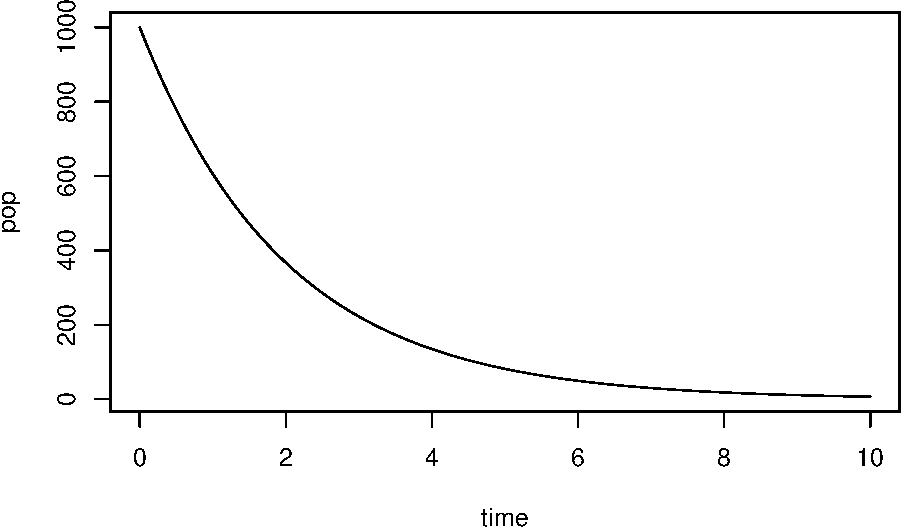
\includegraphics{QuantLife_files/figure-latex/fig-FE-sol-1.pdf}

Notice that it is very similar to the script for numerical solution of a difference equation we saw in \ref{sec:comp14} with the major difference being the presence of a time step, whereas in difference equations the time step is always 1. There is one more important point for the implementation: usually one needs to solve the ODE for a particular length of time \(T\) with a specified time step \(\Delta t\) . This dictates that the required number of iterations be \(T/\Delta t\); in other words, for a given time period the number of time steps is inversely proportional to the time step.

\hypertarget{exercises-17}{%
\subsection{Exercises}\label{exercises-17}}

Consider a slightly different linear ODE:

\[
\frac{dx}{dt} =  0.2 x 
\]

\begin{enumerate}
\def\labelenumi{\arabic{enumi}.}
\tightlist
\item
  Calculate the numeric solution of the ODE for \textbf{one time step} using Forward Euler, for time step dt=0.1, starting with initial value x(0) = 5. Answer: 5.1
\end{enumerate}

\begin{Shaded}
\begin{Highlighting}[]
\CommentTok{\# YOUR CODE HERE}
\end{Highlighting}
\end{Shaded}

\begin{enumerate}
\def\labelenumi{\arabic{enumi}.}
\setcounter{enumi}{1}
\tightlist
\item
  Write a script to solve the ODE using the Forward Euler method based on the outline above. Set the time step dt=0.1 and report the solution \textbf{after 100 time steps}. Answer: 36.22323
\end{enumerate}

\begin{Shaded}
\begin{Highlighting}[]
\CommentTok{\# YOUR CODE HERE}
\end{Highlighting}
\end{Shaded}

\begin{enumerate}
\def\labelenumi{\arabic{enumi}.}
\setcounter{enumi}{2}
\tightlist
\item
  Change the time step to be dt=0.01 and report the solution \textbf{after 1000 time steps}. Answer: 36.87156.
\end{enumerate}

\begin{Shaded}
\begin{Highlighting}[]
\CommentTok{\# YOUR CODE HERE}
\end{Highlighting}
\end{Shaded}

\hypertarget{error-analysis}{%
\subsection{error analysis}\label{error-analysis}}

Numeric solutions of ODE are always approximate, because they use discrete time steps to approximate continuous change (derivatives). Thus numeric solutions always have \emph{error}, which is the difference between the \emph{exact} or \emph{analytic} solution and the numeric solution. If we know the exact solution of an ODE, we can calculate the error using vector subtraction in R. For the same linear ODE we solved above:
\[ 
\frac{dx}{dt} =  -0.5 x 
\]
The analytic solution is \(x(t) = x_0 e^{-0.5t}\), where \(x_0\) is the initial value. Here is an example of computing the numeric solution (as we did above) and then calculating the analytic solution and plotting it:

\begin{Shaded}
\begin{Highlighting}[]
\NormalTok{x0 \textless{}{-}}\StringTok{ }\DecValTok{1000}
\NormalTok{dt \textless{}{-}}\StringTok{ }\FloatTok{0.5} \CommentTok{\# set time step}
\NormalTok{Tmax \textless{}{-}}\StringTok{ }\DecValTok{10} \CommentTok{\# set length of time}
\NormalTok{numstep \textless{}{-}}\StringTok{ }\NormalTok{Tmax}\OperatorTok{/}\NormalTok{dt }\CommentTok{\# assign number of time steps}
\NormalTok{pop \textless{}{-}}\StringTok{ }\KeywordTok{rep}\NormalTok{(x0, numstep}\OperatorTok{+}\DecValTok{1}\NormalTok{) }\CommentTok{\# initialize solution with y0}
\ControlFlowTok{for}\NormalTok{ (i }\ControlFlowTok{in} \DecValTok{1}\OperatorTok{:}\NormalTok{numstep) \{ }\CommentTok{\# do the Euler!}
\NormalTok{    pop[i}\OperatorTok{+}\DecValTok{1}\NormalTok{] \textless{}{-}}\StringTok{ }\NormalTok{pop[i]}\OperatorTok{+}\NormalTok{dt}\OperatorTok{*}\NormalTok{(}\OperatorTok{{-}}\FloatTok{0.5}\OperatorTok{*}\NormalTok{pop[i])}
\NormalTok{\}}
\NormalTok{time \textless{}{-}}\StringTok{ }\KeywordTok{seq}\NormalTok{(}\DecValTok{0}\NormalTok{,Tmax, dt)}
\KeywordTok{plot}\NormalTok{(time, pop, }\DataTypeTok{type=}\StringTok{\textquotesingle{}l\textquotesingle{}}\NormalTok{, }\DataTypeTok{main =} \StringTok{"Numeric and analytic solutions of an ODE"}\NormalTok{) }\CommentTok{\# plot the numeric solution}
\NormalTok{exact \textless{}{-}}\StringTok{ }\NormalTok{x0}\OperatorTok{*}\KeywordTok{exp}\NormalTok{(}\OperatorTok{{-}}\FloatTok{0.5}\OperatorTok{*}\NormalTok{time) }\CommentTok{\# calculate the exact solution}
\KeywordTok{lines}\NormalTok{(time, exact, }\DataTypeTok{col =} \StringTok{\textquotesingle{}red\textquotesingle{}}\NormalTok{) }\CommentTok{\# plot the exact solution}
\KeywordTok{legend}\NormalTok{(}\StringTok{\textquotesingle{}topright\textquotesingle{}}\NormalTok{, }\DataTypeTok{col=}\KeywordTok{c}\NormalTok{(}\StringTok{\textquotesingle{}black\textquotesingle{}}\NormalTok{, }\StringTok{\textquotesingle{}red\textquotesingle{}}\NormalTok{), }\DataTypeTok{lty=}\DecValTok{1}\NormalTok{, }\DataTypeTok{legend =} \KeywordTok{c}\NormalTok{(}\StringTok{\textquotesingle{}numeric\textquotesingle{}}\NormalTok{, }\StringTok{\textquotesingle{}analytic\textquotesingle{}}\NormalTok{))}
\end{Highlighting}
\end{Shaded}

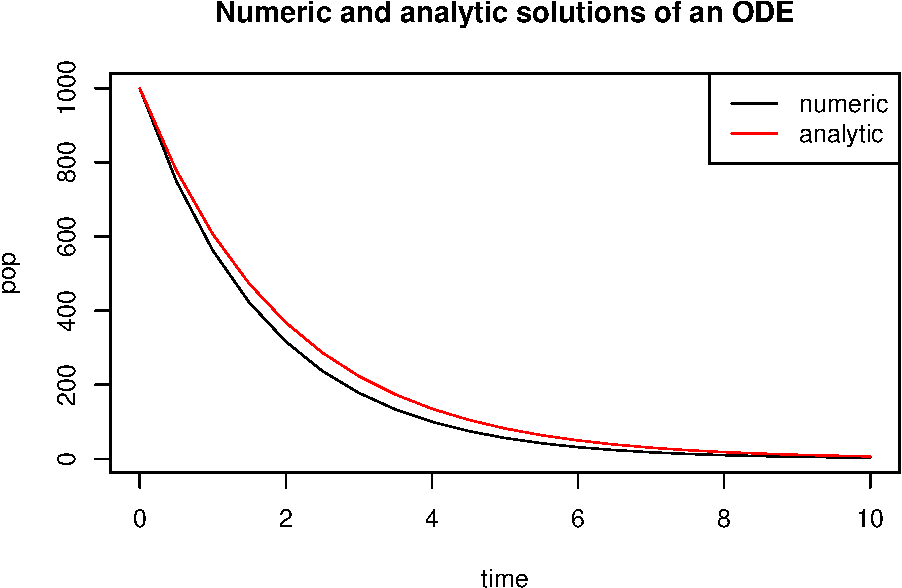
\includegraphics{QuantLife_files/figure-latex/unnamed-chunk-112-1.pdf}

Now we can calculate the error of the numeric solution and plot it:

\begin{Shaded}
\begin{Highlighting}[]
\NormalTok{error \textless{}{-}}\StringTok{ }\KeywordTok{abs}\NormalTok{(exact }\OperatorTok{{-}}\StringTok{ }\NormalTok{pop)}
\KeywordTok{plot}\NormalTok{(time, error, }\DataTypeTok{type =} \StringTok{\textquotesingle{}l\textquotesingle{}}\NormalTok{, }\DataTypeTok{main=}\StringTok{\textquotesingle{}Error of the numeric solution\textquotesingle{}}\NormalTok{)}
\end{Highlighting}
\end{Shaded}

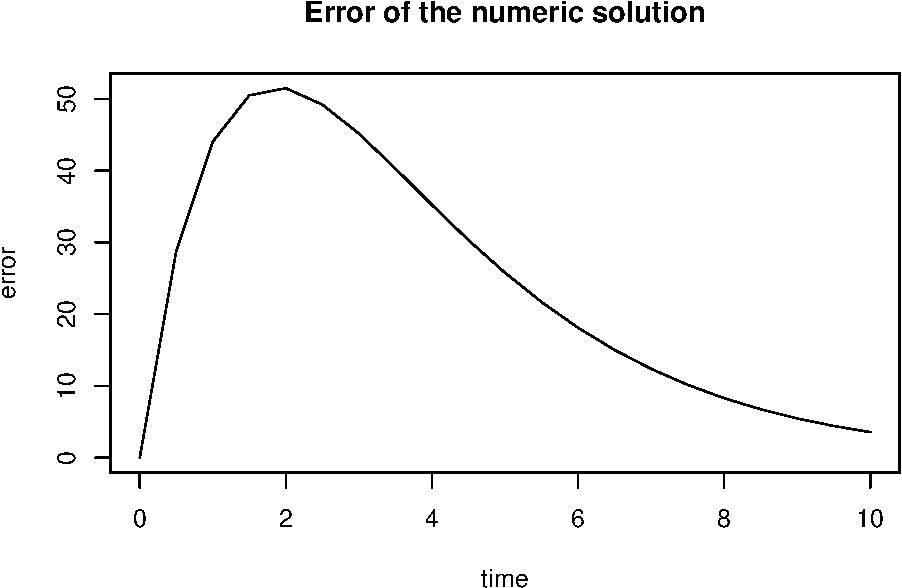
\includegraphics{QuantLife_files/figure-latex/unnamed-chunk-113-1.pdf}

What is the sources of this error? There are at least two distinct sources of error in numerical solutions: a) \index{error!roundoff}\emph{roundoff error} and b) \index{error!truncation}\emph{truncation error}. Roundoff error is caused by computers representing real numbers by a finite string of bits on a computer using what is known as a \index{R programming!floating point}\emph{floating point} representation. In many programming languages variables storing real numbers can be single or double precision, which typically support 24 and 53 significant binary digits, respectively. Any arithmetic operation involving floating point numbers is only approximate, with an error that depends on the way the numbers are stored in the memory. Truncation error is caused by approximations inherent in numerical algorithms, such as Forward Euler, which represent instantaneous rate of change in an ODE with discrete steps and thus are always a bit off from the true analytic solution.

In practice, roundoff error is not a big concern in contemporary computation for most modelers. Truncation error, on the other hand, can cause big problems, but luckily it is within your control. One can decrease the error in the case of finite difference methods by choosing smaller time steps, or by choosing an algorithm with a higher \emph{order of accuracy}, which we'll leave for a more advanced discussion.

Returning specifically to the Forward Euler method, it is called a \index{differential equation!first-order method} \emph{first-order method} because the total error of the solution (after some number of time steps) depends linearly on the time step \(\Delta t\). One can show this by using the Taylor expansion of the solution \(y(t)\) to derive the forward Euler method, with \(\tau(\Delta t)\) representing the truncation error after one time step:
\[y(t+\Delta t) = y(t) +  \Delta t \frac {dy(t) }{dt} + \tau(\Delta t)\]
As you might have learned in calculus, the error remaining after the linear term in the Taylor series is proportional to the the square of the small deviation \(\Delta t\). This only describes the error after 1 time step, but since the errors accumulate every time step, the total error after \(N\) time steps accumulates \(N \tau(\Delta t)\). As we saw in the implementation above, for a given length of time, \(N\) is inversely proportional to \(\Delta t\). Therefore, the total error is proportional to the \(\Delta t\) and so FE is a first-order method.

The exercise above shows that new errors in FE method accumulate in proportion with the time step. The next question is, what happens to these errors over time? Do they grow or dissipate with more iterations? This is known as the stability of a numerical method, and unlike the above question about the order of accuracy, the answer depends on the particular ODE that one needs to solve. Below I show an example of error analysis for a linear ODE:\index{stability!Forward Euler}

\textbf{Example.} To numerically solve the equation \(\dot x = ax\), we substitute the function \(ax\) for the function \(f(x,t)\), and obtain the FE approximation for this particular ODE:
\[y_{i+1} = y_i + \Delta t a y_i = (1+a\Delta t) y_i\]
The big question is what happens to the truncation error: does it grow or decay? To investigate this question, let us denote the error at time \(t_i\) , that is the difference between the true solution \(x(t_i)\) and the approximate solution \(y(t_i)\), by \(\epsilon_i\). It follows that \(y_i = x_i + \epsilon_i\). Then we can wrote the following difference equations involving the error:

\[y_{i+1} = x_{i+1} + \epsilon_{i+1} = (x_i + \epsilon_i) (1+a\Delta t)  = x_i (1+a\Delta t) + \epsilon_i(1+a\Delta t)\]
Let us set aside the terns in the equation that involve \(x\) (since it is just the equation for forward Euler). The remaining difference equation for \(\epsilon\) describes the change in the error:
\[\epsilon_{i+1} = \epsilon_i(1+a\Delta t) \]

This states that the error in this numerical solution is repeatedly multiplied by the constant \((1+a\Delta t)\). As we saw in section \ref{sec:math14}, this linear difference equation has an exponential solution \(\epsilon_n = (1+a\Delta t)^n \epsilon_0\), which decays to 0 if \(|1+a\Delta t| < 1\) or grows without bound if \(|1+a\Delta t| > 1\). The first inequality is called the stability condition for the FE scheme, since it guarantees that the old errors decay over time. Since \(\Delta t >0\), the only way that the left hand side can be less than 1 is if \(a<0\). Therefore, the condition for stability of the FE method for a linear ODE:
\[|1 + a\Delta t| < 1 \Rightarrow \Delta t < -2/a\]

Thus, if \(a>0\), the errors will eventually overwhelm the solution. If \(a<0\), if the time step is small enough (less than \(-2/a\)) then FE is stable. Generally speaking, however, Forward Euler is about the worst method to use for practical numerical solutions of ODEs, due to its low accuracy and to its lack of stability under certain conditions.

\hypertarget{exercises-18}{%
\subsection{Exercises}\label{exercises-18}}

\[
\frac{dx}{dt} =  0.2 x 
\]

\begin{enumerate}
\def\labelenumi{\arabic{enumi}.}
\tightlist
\item
  Calculate the error of the numeric solution of this ODE after one time step with dt=0.1 and initial value x(0) = 5 by subtracting it from the exact (analytic) solution \(x(t) = e^{0.2t}x(0)\), with the same initial value. Answer: about 0.001.
\end{enumerate}

\begin{Shaded}
\begin{Highlighting}[]
\CommentTok{\# YOUR CODE HERE}
\end{Highlighting}
\end{Shaded}

\begin{enumerate}
\def\labelenumi{\arabic{enumi}.}
\setcounter{enumi}{1}
\tightlist
\item
  Compute the error of the two numeric solution over Tmax = 10 by subtracting the numeric solution vector from the analytic solution calculating over the same time vector and report the mean of that error vector. Answers: for dt=0.1 the mean error is 0.722, for dt=0.01 the mean error is 0.0737.
\end{enumerate}

\begin{Shaded}
\begin{Highlighting}[]
\CommentTok{\# YOUR CODE HERE}
\end{Highlighting}
\end{Shaded}

\hypertarget{applications-of-linear-ode-models}{%
\section{Applications of linear ODE models}\label{applications-of-linear-ode-models}}

\label{sec:bio15}

\hypertarget{model-of-pharmacokinetics}{%
\subsection{model of pharmacokinetics}\label{model-of-pharmacokinetics}}

Describing and predicting the dynamics of drug concentration in the body is the goal of \index{kinetics!pharmacology} \emph{pharmacokinetics}. Any drug that humans take goes through several stages: first it is administered (put into the body), then absorbed, metabolized (transformed), and excreted (removed from the body) \citep{rosenbaum_basic_2011}. Almost any drug has a dose at which it has a toxic effect, and most can kill a human if the dose is high enough. Drugs which are used for medical purposes have a \emph{therapeutic range}, which lies between the lowest possible concentration (usually measured in the blood plasma) that achieves the therapeutic effect and the concentration which is toxic. One of the basic questions that medical practitioners need to know is how much and how frequently to administer a drug to maintain drug concentration in the therapeutic range.

The concentration of a drug is a dynamic variable which depends on the rates of several processes, most directly on the rate of administration and the rate of metabolism. Drugs can be \index{kinetics!drug administration} administered through various means (e.g.~orally or intravenously) which influences their rate of absorption and thus how the concentration increases. Once in the blood plasma, drugs are metabolized primarily by enzymes in the liver, converting drug molecules into compounds that can be excreted through the kidneys or the large intestine. The process of \index{kinetics!drug metabolism} *metabolism proceeds at a rate that depends on both the concentration of the drug and on the enzyme that catalyzes the reaction. For some drugs the metabolic rate may be constant, or independent of the drug concentration, since the enzymes are already working at full capacity and can't turn over any more reactions, for example alcohol is metabolized at a constant rate of about 1 drink per hours for most humans. Figure \ref{fig:ch15_drug_conc}a shows the time plots of the blood alcohol concentration for 4 males who ingested different amounts of alcohol, and the curves are essentially linear with the same slope after the peak. For other drugs, if the plasma concentration is low enough, the enzymes are not occupied all the time and increasing the drug concentration leads to an increase in the rate of metabolism. One can see this behavior in the metabolism of the anti-depressant drug bupropion in figure \ref{fig:ch15_drug_conc}b, where the concentration curve shows a faster decay rate for higher concentration of the drug than for lower concentration. In the simplest case, the rate of metabolism is linear, or proportional to the concentration of the drug, with proportionality constant called the first-order metabolic rate.

\begin{figure}
\centering
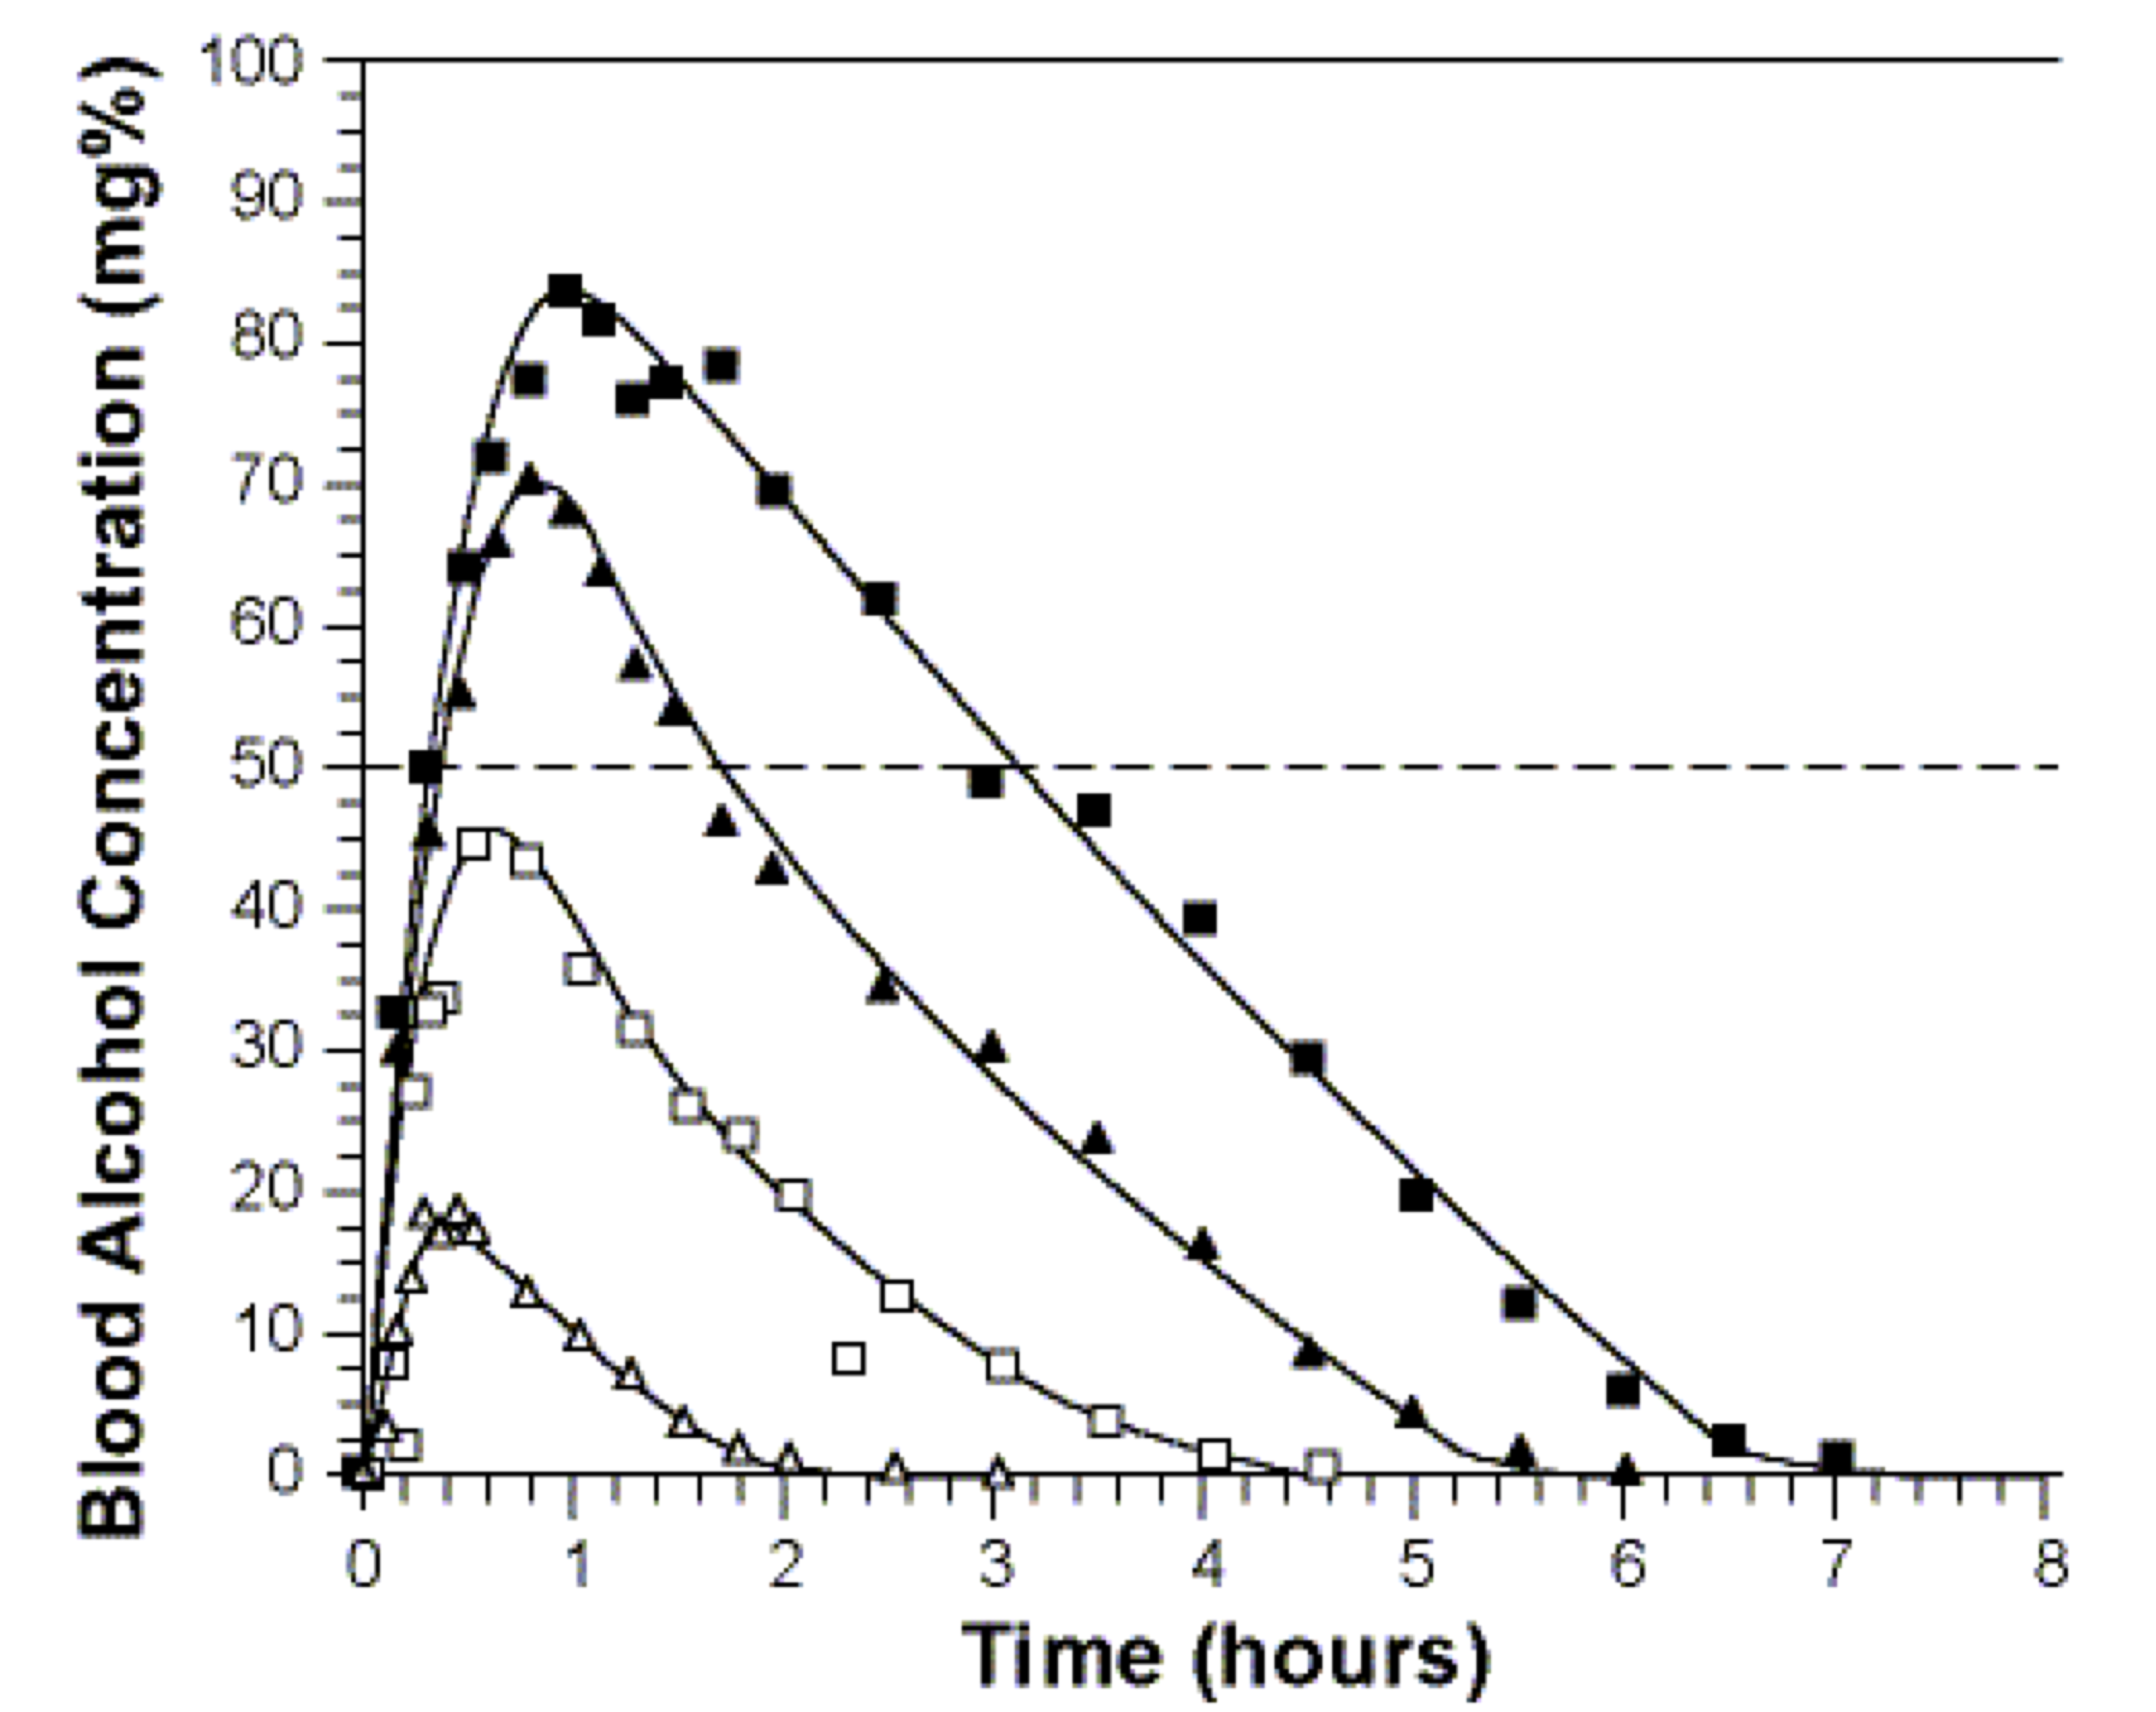
\includegraphics{ch15/aa35graf.png}
\caption{Blood alcohol content after ingesting different numbers of drinks, from 4 in the top curve to 1 in the bottom (figure from the National Institute on Alcohol Abuse and Alcoholism in public domain)}
\end{figure}

\begin{figure}
\centering
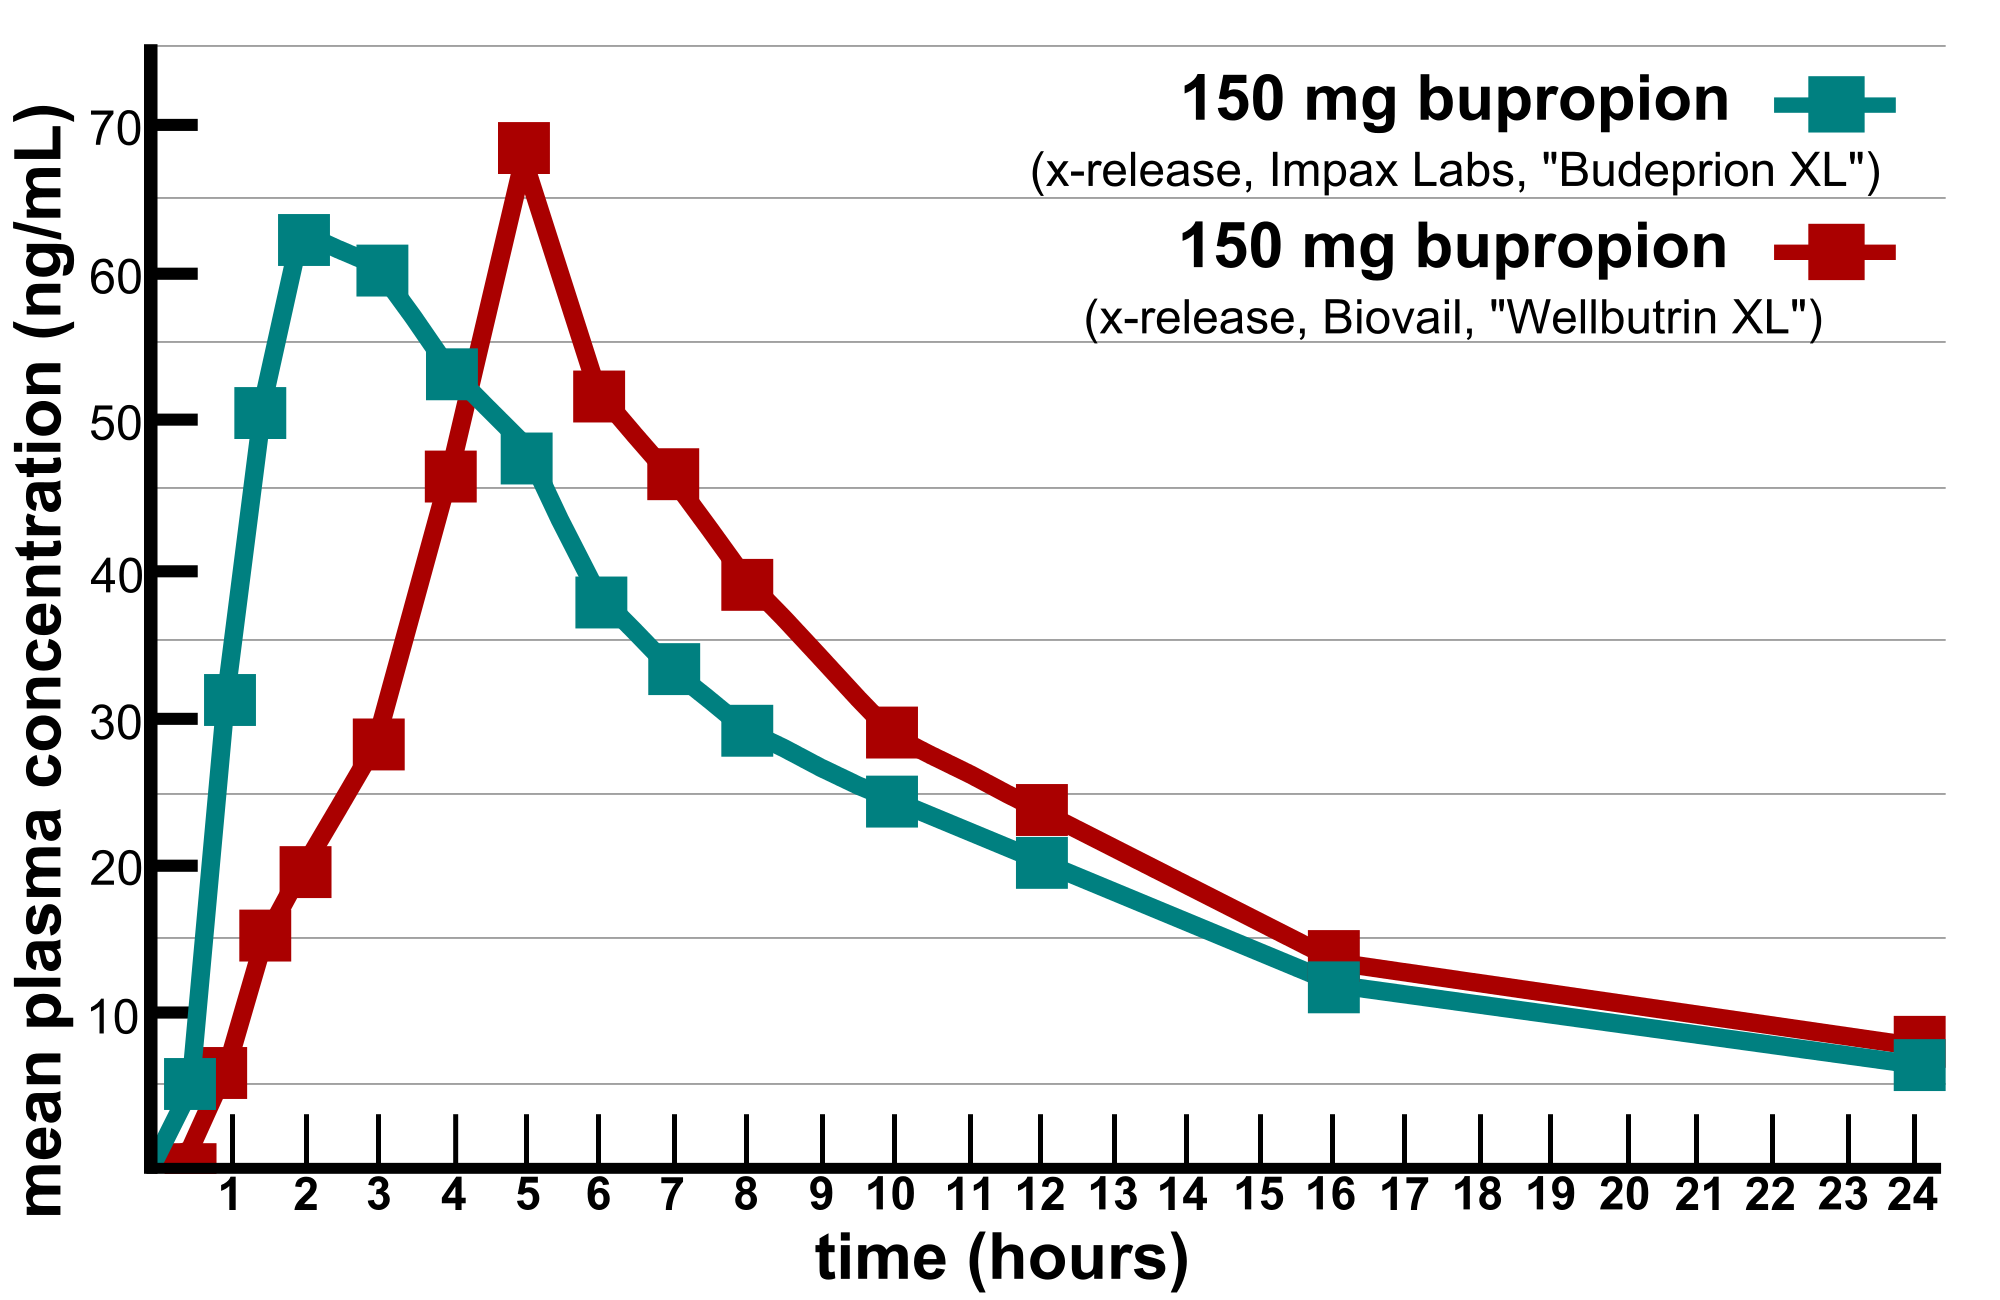
\includegraphics{ch15/2000px-Bupropion_bioequivalency.png}
\caption{Blood concentration of bupropion for two different drugs in clinical trials (image by CMBJ based on FDA data under CC-BY 3.0 via Wikimedia Commons)}
\end{figure}

Let us build an ODE model for a simplified pharmacokinetics situation. Suppose that a drug is administered at a constant rate of \(M\) (concentration units per time unit) and that it is metabolized at a rate proportional to its plasma concentration \(C\) with metabolic rate constant \(k\). Then the ODE model of the concentration of the drug over time \(C(t)\) is:
\[ \frac{dC}{dt} = M - kC\]
The two rate constants \(M\) and \(k\) have different dimensions, which you should be able to determine yourself. The ODE can be solved using the separate-and-integrate method:

\begin{enumerate}
\def\labelenumi{\arabic{enumi}.}
\tightlist
\item
  Divide both sides by the right hand side \(M-kC\), and multiply both sides by the differential \(dt\)
  \[ \frac{dC}{M-kC} = dt\]
\item
  integrate both sides with respect to the different variables, don't forget the integration constant!
  \[ \int \frac{dC}{M-kC} = \int dt \Rightarrow\]
  \[ -\frac{1}{k} \log |M-kC| = t + A\]
\item
  solve for the dependent variable \(C(t)\)
  \[ \exp(\log |M-kC| ) = -\exp(kt +A) \Rightarrow \]
  \[  M - kC = B e^{-kt} \Rightarrow \]
  \[ C(t) = \frac{M}{k}- Be^{-kt}\]
  Notice that I changed the values of integration constants \(A\) and \(B\) during the derivation, which shouldn't matter because they have not been determined yet.
\item
  plug in \(t=0\) and use the initial value \(x(0)\) to solve for the integration constant
  If we know the initial value \(C(0) = C_0\), then we can plug it in and get the following algebraic expression:
  \[ C_0 =  \frac{M}{k} - B \Rightarrow \]
  \[ B = C_0 -  \frac{M}{k}\]
  Then the complete solution is:
  \[ C(t) =  \frac{M}{k} - (C_0- \frac{M}{k})e^{-kt}\]
\end{enumerate}

The solution predicts that after a long time the plasma concentration will approach the value \(M/k\), since the exponential term decays to zero. Notice that mathematically this is the same type of solution we obtained in equation \ref{eq:ch15_ode_sol} for a generic linear ODE with a constant term.

\hypertarget{discussion-questions-2}{%
\subsection{Discussion questions}\label{discussion-questions-2}}

\begin{enumerate}
\def\labelenumi{\arabic{enumi}.}
\item
  Describe in words the dependence of the long-term plasma concentration of the drug on the \index{parameter!drug metabolism}parameters. Does this prediction make intuitive sense?
\item
  Explain in practical terms the assumption that the administration of the drug results in a constant rate of growth of the concentration. Under what circumstances does this match reality?\}
\item
  Explain in practical terms the assumption that the drug metabolism rate is proportional to the plasma concentration. Under what circumstances does this match reality?\}
\item
  Discuss how you could modify the ODE model to describe other circumstances, or to add other effects to it.\}
\item
  The following questions encourage you to think critically about the pharmacokinetic model above.\}
\end{enumerate}

\hypertarget{r-assignment-5}{%
\section{R Assignment}\label{r-assignment-5}}

In this part you will solve the linear population model ODE:
\[ \frac{dN}{dt} = (b-d) N \]
The model parameters are per capita birth and death rates (b and d, respectively), which may be expressed in percent population change per year (e.g.~d= 0.12 is a death rate of 12\% per year). Assume that the initial population is 500 individuals, and perform the following tasks:

\begin{enumerate}
\def\labelenumi{\arabic{enumi}.}
\tightlist
\item
  Write a Forward Euler script to solve this ODE for any given values of b and d (they should be inputs into your defining function).
\end{enumerate}

\begin{enumerate}
\def\labelenumi{\alph{enumi})}
\tightlist
\item
  Set b=0.5 and d=0.12, plot the numeric solution, and report whether the solution behaves as you would expect it to, for Tmax=50 and dt=0.1. Describe the behavior of the solution of the ODE over time.
\end{enumerate}

\begin{Shaded}
\begin{Highlighting}[]
\CommentTok{\#YOUR CODE HERE}
\end{Highlighting}
\end{Shaded}

YOUR ANSWERS HERE

\begin{enumerate}
\def\labelenumi{\alph{enumi})}
\setcounter{enumi}{1}
\tightlist
\item
  Change the birth rate to b=0.01 and calculate the solution with the same initial value and same values of Tmax and dt. Plot the solution, describe its behavior, and compare its behavior to the one in the previous task.
\end{enumerate}

\begin{Shaded}
\begin{Highlighting}[]
\CommentTok{\#YOUR CODE HERE}
\end{Highlighting}
\end{Shaded}

YOUR ANSWERS HERE

\begin{enumerate}
\def\labelenumi{\alph{enumi})}
\setcounter{enumi}{2}
\tightlist
\item
  Keeping b=0.01 and d=0.12, calculate the numeric solution of the ODE with different time steps: dt = 1, 5, 10. Plot the solutions and report how they behave for larger values of the time step. What time step would you consider optimal for this problem?
\end{enumerate}

\begin{Shaded}
\begin{Highlighting}[]
\CommentTok{\#YOUR CODE HERE}
\end{Highlighting}
\end{Shaded}

YOUR ANSWERS HERE

\begin{enumerate}
\def\labelenumi{\arabic{enumi}.}
\setcounter{enumi}{1}
\item
  \begin{enumerate}
  \def\labelenumii{\alph{enumii})}
  \tightlist
  \item
    Use your FE script to compute and plot the numerical solution of the ODE for b=0.5, d=0.12, with dt=0.1 over the span of 0 to 50 years. Calculate the analytic solution (see section 15.2) from the same time vector (0 to 50 with time step 0.1) and overlay the analytic solution on the same plot. Calculate and plot the vector of errors (absolute difference between the analytic and numerical solution) and plot it over time. Describe how the error behaves in this plot.
  \end{enumerate}
\end{enumerate}

\begin{Shaded}
\begin{Highlighting}[]
\CommentTok{\#YOUR CODE HERE}
\end{Highlighting}
\end{Shaded}

YOUR ANSWERS HERE

\begin{enumerate}
\def\labelenumi{\alph{enumi})}
\setcounter{enumi}{1}
\tightlist
\item
  Keeping the same parameters b=0.5 and d=0.12, calculate the mean error of the numerical solution by using the mean function on the absolute difference between the analytic solution vector and the numerical solution vector, for three values of the time step: dt=1, 0.1, 0.01 and Tmax=50. Report how the reduction in the error compares with each decrease in the time step.
\end{enumerate}

\begin{Shaded}
\begin{Highlighting}[]
\CommentTok{\#YOUR CODE HERE}
\end{Highlighting}
\end{Shaded}

YOUR ANSWERS HERE

\begin{enumerate}
\def\labelenumi{\arabic{enumi}.}
\setcounter{enumi}{2}
\item
  \begin{enumerate}
  \def\labelenumii{\alph{enumii})}
  \tightlist
  \item
    Use the birth rate to b=0.01, keep d=0.12 and again calculate and plot the numerical solution along with the analytic solution for the same values of Tmax and dt. Calculate and plot the vector of errors (absolute difference between the analytic and numerical solution) and plot it over time in a separate plot. Describe how the error behaves in this plot.
  \end{enumerate}
\end{enumerate}

\begin{Shaded}
\begin{Highlighting}[]
\CommentTok{\#YOUR CODE HERE}
\end{Highlighting}
\end{Shaded}

YOUR ANSWERS HERE

\begin{enumerate}
\def\labelenumi{\alph{enumi})}
\setcounter{enumi}{1}
\tightlist
\item
  Calculate the mean error of the numerical solution for three values of the time step: dt=1, 0.1, 0.01 with Tmax=50. Report how the reduction in the error compares with each decrease in the time step.
\end{enumerate}

\begin{Shaded}
\begin{Highlighting}[]
\CommentTok{\#YOUR CODE HERE}
\end{Highlighting}
\end{Shaded}

YOUR ANSWERS HERE

\hypertarget{graphical-analysis-of-ordinary-differential-equations}{%
\chapter{Graphical analysis of ordinary differential equations}\label{graphical-analysis-of-ordinary-differential-equations}}

\chaptermark{analysis of ODEs}

\begin{quote}
I find the great thing in this world is not so much where we stand, as in what direction we are moving.\\
-- Oliver Wendell Holmes, Sr., \emph{The Autocrat of the Breakfast Table}
\end{quote}

We now proceed from linear ODEs to more complicated nonlinear equations. In contrast to linear differential equations, which can be solved in general, nonlinear differential equations may not be solvable even theoretically. Even though the solutions cannot be written down, they exist and can exhibit much more interesting behaviors than the exponential solutions we have seen. When solutions cannot be found on paper, we have two options: 1) use qualitative or graphical tools, such as finding equilibrium points and their stability, to predict the long-term dynamics of the solution; 2) construct numerical solutions that approximate the true solution. In this chapter we concentrate on the qualitative approach to analyzing ODEs, which allows one to predict the behavior of solutions of any autonomous ODE based on the graph of the defining function of the equation. After working through this chapter you will learn to do the following:

\begin{itemize}
\item
  find equilibrium values of an ODE
\item
  analyze the stability of equilibria based on the graph of the defining function
\item
  write down stability conditions analytically
\item
  use graphical techniques to predict the behavior of the solution of a difference equation without solving it
\item
  understand basic compartment epidemiology models
\end{itemize}

\hypertarget{building-nonlinear-odes}{%
\section{Building nonlinear ODEs}\label{building-nonlinear-odes}}

\label{sec:model16}

The simple, linear population growth models we have seen in the last two chapters assume that the per capita birth and death rates are constant, that is, they stay the same regardless of population size. The solutions for these models either grow or decay exponentially, but in reality, populations do not grow without bounds. It is generally true that the larger a population grows, the more scarce the resources, and survival becomes more difficult. For larger populations, this could lead to higher death rates, or lower birth rates, or both.

How can we incorporate this effect into a quantitative model? We will assume there are separate birth and death rates, and that the birth rate declines as the population grows, while the death rate increases. Suppose there are inherent birth rates \(b\) and \(d\), and the overall birth and death rates \(B\) and \(D\) depend linearly on population size \(P\): \(B = b - aP\) and \(D = d + cP\).

To model the rate of change of the population, we need to multiply the rates \(B\) and \(D\) by the population size \(P\), since each individual can reproduce or die. Also, since the death rate \(D\) decreases the population, we need to put a negative sign on it. The resulting model is:
\[ \dot P = BP - DP = [(b-d)-(a+c)P]P \]

The parameters of the model, the constants \(a,b,c,d\), have different meanings. Performing \index{dimensional analysis} dimensional analysis, we find that \(b\) and \(d\) have the dimensions of \(1/[t]\), the same as the rate \(r\) in the exponential growth model. However, the dimensions of \(a\) (and \(c\)) must obey the relation: \([P]/[t] = [a][P]^2\), and thus,

\[[a]=[c] = \frac{1}{[t][P]}\]

This shows that the constants \(a\) and \(c\) have to be treated differently than \(b\) and \(d\). Let us define the inherent growth rate of the population, to be \(r_0=b-d\) (if the death rate is greater than the birth rate, the population will inherently decline). Then let us introduce another constant \(K\), such that \((a+c)=r_0/K\). It should be clear from the dimensional analysis that \(K\) has units of \(P\), population size. Now we can write down the logistic equation in the canonical form:
\begin{equation}
\dot P = r\left(1-\frac{P}{K}\right)P
\label{eq:log_cont_model}
\end{equation}
This model can be re-written as \(\dot P = aP -bP^2\), \index{model!logistic}\index{differential equation!logistic}so it is clear that there is a \emph{linear term} (\(aP\)) and a \emph{nonlinear term} (\(-bP^2\)). When \(P\) is sufficiently small (and positive) the linear term is greater, and the population grows. When \(P\) is large enough, the nonlinear term wins and the population declines. \index{nonlinear!differential equation}

It should be apparent that there are two fixed points, at \(P=0\) and at \(P=K\). The first one corresponds to a population with no individuals. On the other hand, \(K\) signifies the population at which the negative effect of population size balances out the inherent population growth rate, and is called the \index{population!carrying capacity} \emph{carrying capacity} of a population in its environment \citep{otto_biologists_2007}. We will analyze the qualitative behavior of the solution, without writing it down, in the next section of this chapter.

\hypertarget{qualitative-analysis-of-odes}{%
\section{Qualitative analysis of ODEs}\label{qualitative-analysis-of-odes}}

\label{sec:math16}

In this section we will analyze the behavior of solutions of an autonomous ODE without solving it on paper. Generally, ODE models for realistic biological systems are nonlinear, and most nonlinear differential equations cannot be solved analytically. We can make predictions about the behavior, or \emph{dynamics} of solutions by considering the properties of the \index{differential equation!defining function} \emph{defining function}, which is the function on the right-hand-side of a general autonomous ODE:
\[ \frac{dx}{dt} = f(x)\]

\hypertarget{graphical-analysis-of-the-defining-function}{%
\subsection{graphical analysis of the defining function}\label{graphical-analysis-of-the-defining-function}}

The defining function relates the value of the solution variable \(x\) to its rate of change \(dx/dt\). For different values of \(x\), the rate of change of \(x(t)\) is different, and it is defined by the function \(f(x)\). There are only three options:

\begin{itemize}
\item
  if \(f(x) > 0\), \(x(t)\) is increasing at that value of \(x\)
\item
  if \(f(x) < 0\), \(x(t)\) is decreasing at that value of \(x\)
\item
  if \(f(x) = 0\), \(x(t)\) is not changing that value of \(x\)
\end{itemize}

To determine for which values of \(x\) the solution \(x(t)\) increases and decreases, it enough to look at the plot of \(f(x)\). On the intervals where the graph of \(f(x)\) is above the \(x\)-axis \(x(t)\) increases, on the intervals where the graph of \(f(x)\) is below the \(x\)-axis, \(x(t)\) decreases. The roots (zeros) of \(f(x)\) are special cases, they separate the range of \(x\) into the intervals where the solution grows and and where it decreases. This seems exceedingly simple, and it is, but it provides specific information about \(x(t)\), without knowing how to write down its formula.

For an autonomous ODE with one dependent variable, the direction of the rate of change prescribed by the differential equation can be graphically represented by sketching the \index{differential equation!flow} \emph{flow on the line} of the dependent variable. The flow stands for the direction of change at every point, specifically increasing, decreasing, or not changing. The flow is plotted on the horizontal x-axis, so if \(x\) is increasing, the flow will be indicated by a rightward arrow, and if it is decreasing, the flow will point to the left. The fixed points separate the regions of increasing (rightward) flow and decreasing (leftward) flow.

\begin{figure}

{\centering 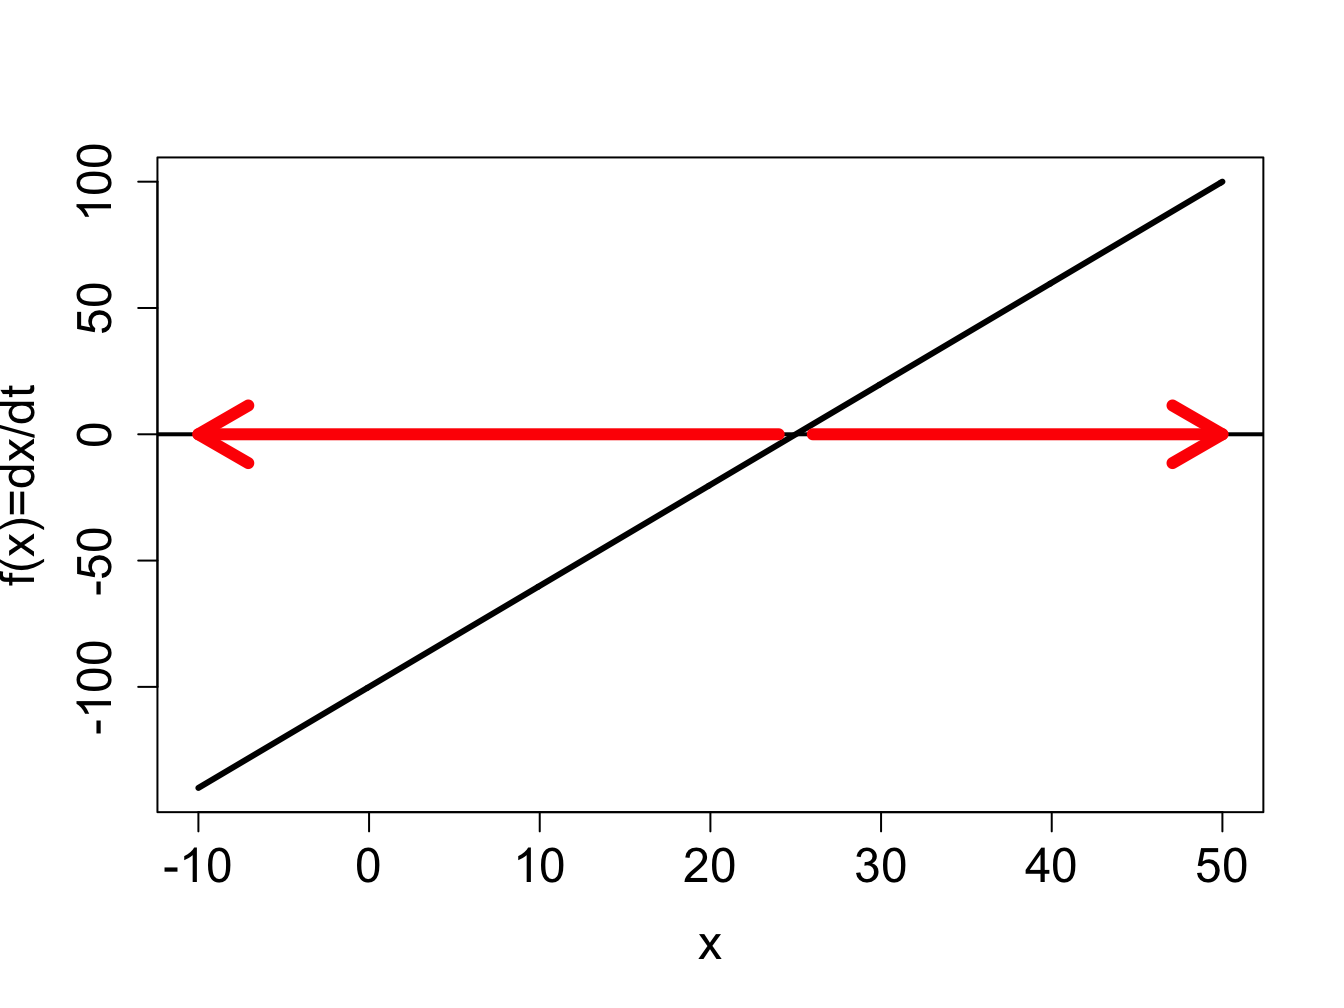
\includegraphics[width=0.5\linewidth]{QuantLife_files/figure-latex/ch7-flow1-1} 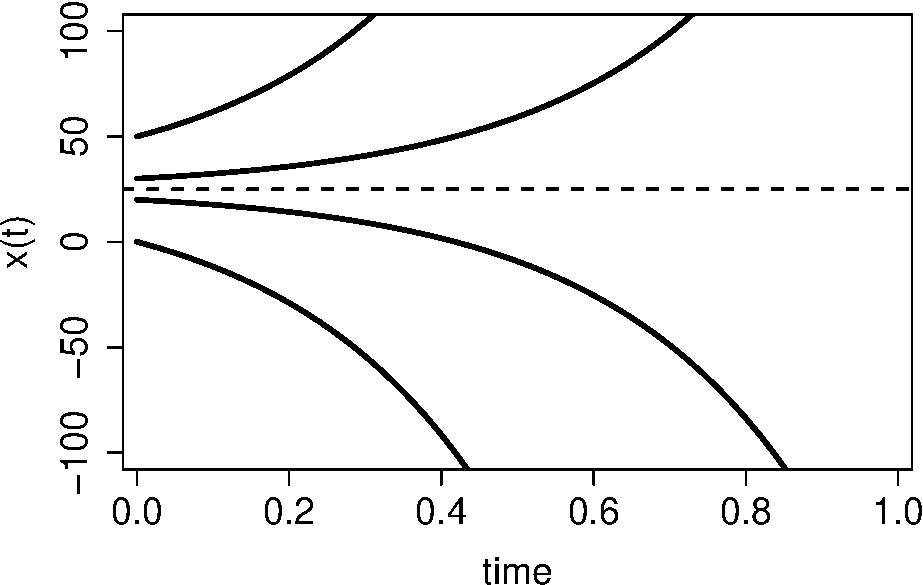
\includegraphics[width=0.5\linewidth]{QuantLife_files/figure-latex/ch7-flow1-2} 

}

\caption{a) plot of the defining function of the ODE dx/dt = 4x-100 with direction of flow x(t) indicated with arrows on the x-axis; b) plot of solutions x(t) of the ODE staring with four initial values.}\label{fig:ch7-flow1}
\end{figure}

\textbf{Example.} Consider a linear ODE the likes of which we have solved in section \ref{sec:math15}:
\[\frac{dx}{dt} = 4x -100\]
The defining function is a straight line vs.~\(x\), its graph is shown in figure \ref{fig:ch16_flow_linear}a. Based on this graph, we conclude that the solution decreases when \(x<25\) and increases when \(x>25\). Thus we can sketch the solution \(x(t)\) over time, without knowing its functional form. The dynamics depends on the initial value: if \(x(0)<25\), the solution will keep decreasing without bound, and go off to negative infinity; if \(x(0)>25\), the solution will keep decreasing without bound, and go off to positive infinity. This is shown by plotting numerical solutions of this ODE for several initial values in figure \ref{fig:ch16_flow_linear}b. The dotted line shows the location of the special value of 25 which separates the interval of growth from the interval of decline.

\textbf{Example.} Now let us analyze a nonlinear ODE, specifically the logistic model with the following parameters:
\[\frac{dP}{dt} =0.3P\left(1-\frac{P}{40}\right)\]

The defining function is a downward-facing parabola with two roots at \(P=0\) and \(P=40\), as shown in figure \ref{fig:ch16_flow_logistic}a. Between the two roots, the defining function is positive, which means the derivative \(dP/dt\) is positive too, so the solution grows on that interval. For \(P<0\) and \(P>40\), the solution decreases. Therefore, we can sketch the graphs of the solution \(P(t)\) starting with different initial conditions, as show in figure \ref{fig:ch16_flow_logistic}b.

To summarize, the defining function of the ODE determines the rate of change of the solution \(x(t)\) depending on the value of \(x\). The graphical approach to finding areas of right and left flow is based on graphing the function \(f(x)\), and dividing the x-axis based on the sign of \(f(x)\). In the areas where \(f(x) > 0\), its graph is above the x-axis, and the flow is to the right; conversely, when \(f(x) < 0\), its graph is below the x-axis, and the flow is to the left. The next subsection puts this approach in a more analytic framework.

\begin{figure}

{\centering 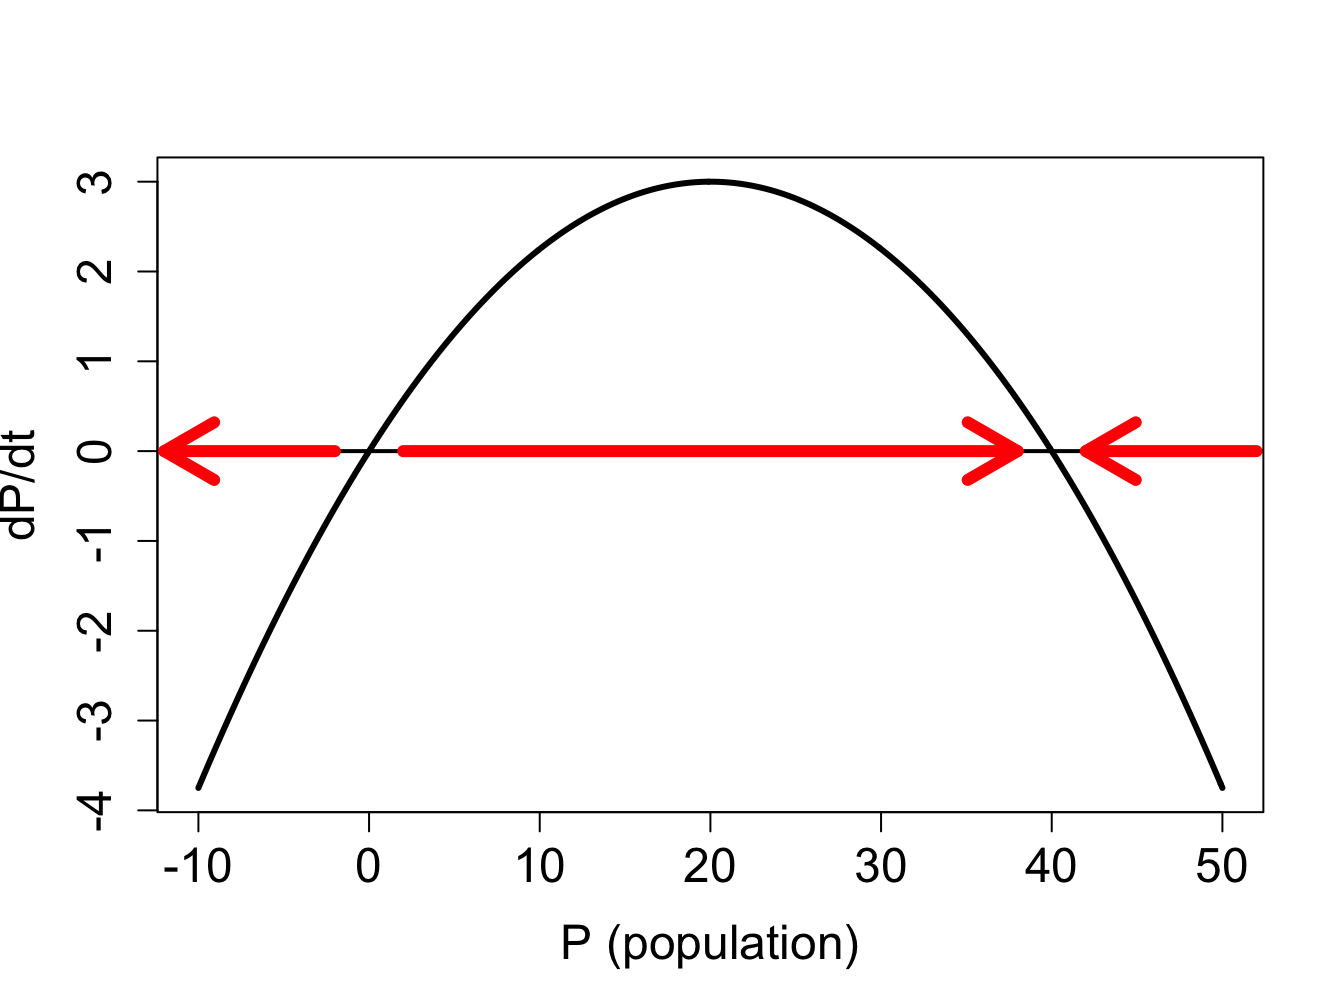
\includegraphics[width=0.5\linewidth]{QuantLife_files/figure-latex/ch7-flow2-1} 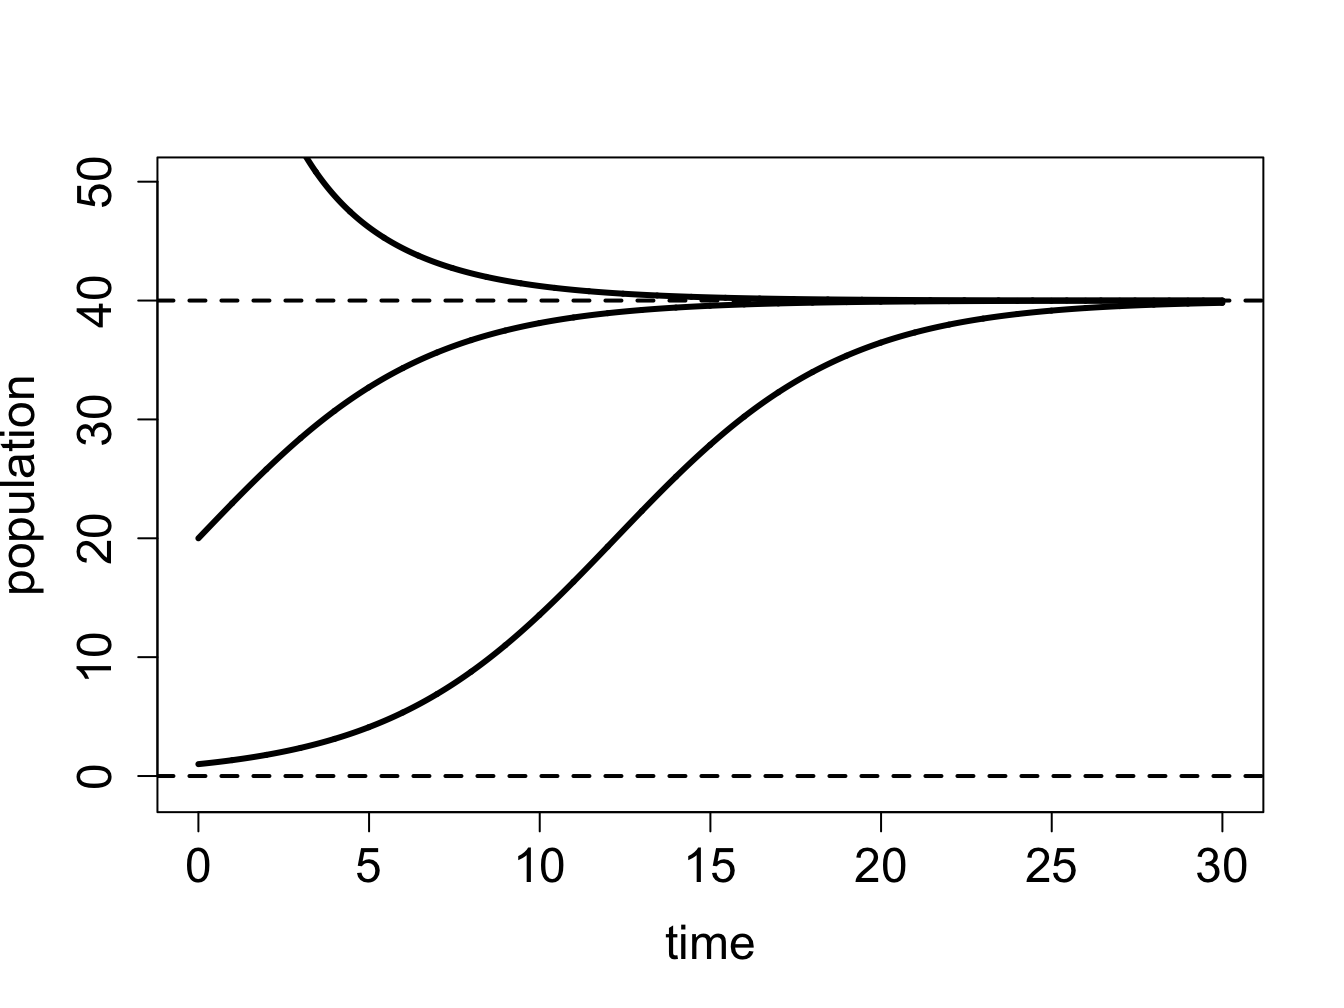
\includegraphics[width=0.5\linewidth]{QuantLife_files/figure-latex/ch7-flow2-2} 

}

\caption{a) plot of the defining function of the ODE $dP/dt = 0.3P(1-P/40)$ with direction of flow of P(t) indicated with arrows on the P-axis; b) plot of solutions P(t) of the ODE staring with three initial values}\label{fig:ch7-flow2}
\end{figure}

\hypertarget{fixed-points-and-stability}{%
\subsection{fixed points and stability}\label{fixed-points-and-stability}}

We have seen that the dynamics of solutions of differential equations depend on the initial value of the dependent variable: for some values the solution increases, for others it decreases, and for intermediate values it remains the same. Those special values separating intervals of increase and decrease are called fixed points (or equilibria), and the first step to understanding the dynamics of an ODE is finding its fixed points. A fixed point is a value of the solution at which the dynamical system stays constant, thus, the derivative of the solution must be zero. Here is the formal definition:
\begin{definition}
\protect\hypertarget{def:def-fp}{}{\label{def:def-fp} }For an ordinary differential equation \(\dot x = f(x)\), a point \(x^*\) which satisfies \(f(x^*)=0\) is called a \emph{fixed point} or \emph{equilibrium}, and the solution with the initial condition \(x(0)=x^*\) is constant over time \(x(t)=x^*\).
\end{definition}

\textbf{Example.} The linear equation \(\dot x = rx\) has a single fixed point at \(x^* = 0\). For a more interesting example, consider a logistic equation: \(\dot x = x - x^2\). Its fixed points are the solutions of \(x - x^2 = 0\), therefore there two fixed points: \(x^* = 0, 1\). We know that if the solution has either of the fixed points as the initial condition, it will remain at that value for all time.

Locating the fixed points is not sufficient to predict the global behavior of the dynamical system, however. What happens to the solution of a dynamical system if the initial condition is very close to an equilibrium, but not precisely at it? Put another way, what happens if the equilibrium is perturbed? The solution may be attracted to the equilibrium value, that is, it approaches it ever-closer, or else it is not. In the first case, this is called a stable equilibrium, because a small perturbation does not dramatically change the long-term behavior of the solution. In the latter case, the equilibrium is called unstable, and the solution perturbed from the equilibrium never returns. These concepts are formalized in the following definition

\begin{definition}
\protect\hypertarget{def:def-stable}{}{\label{def:def-stable} }A fixed point \(x^*\) of an ODE \(\dot x = f(x)\) is called a \emph{stable} fixed point (or sink) if for a sufficiently small number \(\epsilon\), the solution \(x(t)\) with the initial condition \(x_0 = x^* + \epsilon\) approaches the fixed point \(x^*\) as \(t \rightarrow \infty\). If the solution \(x(t)\) does not approach \(x^*\) for all nonzero \(\epsilon\), the fixed point is called an \emph{unstable} fixed point (or source).
\end{definition}

To determine whether a fixed point is stable analytically we use the approach called \index{differential equation!linearization}\index{linearization!differential equation} \emph{linearization}, which involves replacing the function \(f(x)\) with a linear approximation. Let us define \(\epsilon(t)\) to be the deviation of the solution \(x(t)\) from the fixed point \(x^*\), so we can write \(x(t) = x^* + \epsilon(t)\). Assuming that \(\epsilon(t)\) is small, we can write the function \(f(x)\) using Taylor's formula:
\[ f(x^*+\epsilon(t))= f(x^*)+f'(x^*) \epsilon(t) + ... = f'(x^*) \epsilon(t) + ... \]

The term \(f(x^*)\) vanished because it is zero by definition \ref{def:ch16_fixedpt} of a fixed point. The ellipsis indicates all the terms of order \(\epsilon(t)^2\) and higher, which are very small if \(\epsilon(t)\) is small, and thus can be neglected. Thus, we can write the following approximation to the ODE \(\dot x = f(x)\) near a fixed point:

\[ \dot x =  \frac{d(x^* + \epsilon(t))}{dt} = \dot \epsilon(t) =  f'(x^*) \epsilon(t)\]

Thus we replaced the complicated nonlinear ODE near a fixed point with a linear equation, which approximates the dynamics of the deviation \(\epsilon(t)\) near the fixed point \(x^*\); note that the derivative \(f'(x^*)\) is a constant for any given fixed point. In section \ref{sec:math15} we classified the behavior of solutions for the general linear ODE \(\dot x = rx\), and now we apply this classification to the behavior of the deviation \(\epsilon(t)\). If the multiple \(f'(x^*)\) is positive, the deviation \(\epsilon(t)\) is growing, the solution is diverging away from the fixed point, and thus the fixed point is unstable. If the multiple \(f'(x^*)\) is negative, the deviation \(\epsilon(t)\) is decaying, the solution is converging to the fixed point, and thus the fixed point is stable. Finally, there is the borderline case of \(f'(x^*) = 0\) which is inconclusive, and the fixed point may be either stable or unstable. The \index{differential equation!stability analysis} derivative stability analysis is summarized in the following:

\begin{itemize}
\tightlist
\item
  \(f'(x^*) > 0\): the slope of \(f(x)\) at the fixed point is positive, then the fixed point is \textbf{unstable}.
\item
  \(f'(x^*) < 0\): the slope of \(f(x)\) at the fixed point is negative, then the fixed point is \textbf{stable}.
\item
  \(f'(x^*) = 0\): stability cannot be determined from the derivative.
\end{itemize}

Therefore, knowing the derivative or the slope of the defining function at the fixed point is enough to know its stability. If the derivative has the discourtesy of being zero, the situation is tricky, because then higher order terms that we neglected make the difference. We will mostly avoid such borderline cases, but they are important in some applications \citep{strogatz_nonlinear_2001}.

\textbf{A word of caution:} The derivative of the defining function \(f'(x)\) is not the second derivative of the solution \(x(t)\). This is a common mistake, because the function \(f(x)\) is equal to the time derivative of \(x(t)\). However, the derivative \(f'(x)\) is not with respect to time, it is with respect to x, the dependent variable. In other words, it reflects the slope of the graph of the defining function \(f(x)\), not the curvature of the graph of the solution \(x(t)\).

To summarize, here is an outline of the steps for analyzing the behavior of solutions of an autonomous one-variable ODE. These tasks can be accomplished either by plotting the defining function \(f(x)\) and finding the fixed points and their stability based on the plot, or by solving for the fixed points on paper, then finding the derivative \(f'(x)\) and plugging in the values of the fixed points to determine their stability. Either approach is valid, but the analytic methods are necessary when dealing with models that have unknown parameter values, which makes it impossible to represent the defining function in a plot.

\hypertarget{outline-of-qualitative-analysis-of-an-ode}{%
\subsection{Outline of qualitative analysis of an ODE}\label{outline-of-qualitative-analysis-of-an-ode}}

\begin{itemize}
\item
  find the fixed points by setting the defining function \(f(x)=0\) and solving for values of \(x^*\)
\item
  divide the domain of \(x\) into intervals separated by fixed points \(x^*\)
\item
  determine on which interval(s) the solution \(x(t)\) is increasing and on which it is decreasing
\item
  use derivative stability analysis (graphically or analytically) to determine which fixed points are stable
\item
  sketch the solutions \(x(t)\) starting at different initial values, based on the stability analysis and whether the solution is increasing or decreasing in a particular interval
\end{itemize}

\textbf{Example: linear model.} Consider the linear ODE that we analyzed above \(dx/dt = 4x -100\). Let us go through the steps of qualitative analysis:

\begin{itemize}
\item
  find the fixed points by setting the defining function to 0: \(0 = 4x -100\), so there is only one fixed point \(x^* = 25\)
\item
  divide the domain of \(x\) into intervals separated by fixed points \(x^*\): the intervals are \(x<25\) and \(x>25\)
\item
  the solution is decreasing on the interval \(x<25\) because \(f(x)<0\) there, and the solution is increasing on the interval \(x>25\) because \(f(x)>0\)
\item
  the derivative \(f'(x)\) at the fixed point is 4, so the fixed point is \emph{unstable}
\item
  solutions \(x(t)\) starting at different initial values are shown in figure \ref{fig:ch16_flow_linear}b and they behave as follows: solutions with initial values below \(x^*=25\) decreasing, and those with initial values above \(x^*=25\) increasing.
\end{itemize}

** Example: logistic model.** \index{model!logistic}\index{function!logistic} Consider the logistic model from the previous subsection, \(dP/dt =0.3P(1-P/40)\). We have analyzed the stability of the two fixed points using the plot in figure \ref{fig:ch16_flow_logistic}, and saw that the flow takes the solution away from \(P=0\), and toward \(P=K\), thus the first fixed point is unstable, while the second is stable. Let us repeat the analysis using analytic tools:

\begin{itemize}
\item
  find the fixed points by setting the defining function to 0: \(0 = 0.3P(1-P/40)\). The two solutions are \(P^*=0\) and \(P^*=40\).
\item
  divide the domain of \(P\) into intervals separated by fixed points \(P^*\): the intervals are \(P<0\); \(0<P<40\); and \(P>40\)
\item
  the solution is decreasing on the interval \(P<0\) because \(f(P)<0\) there, the solution is increasing on the interval \(0<P<40\) because \(f(P)>0\), and the solution is decreasing for \(P>40\) because \(f(P)<0\) there
\item
  the derivative is \(f'(P)=0.3-0.3P/20\); since \(f'(0)=0.3 > 0\), the fixed point is \emph{unstable}; since \(P'(40)=-0.3<0\), the fixed point is \emph{stable}
\item
  solutions \(P(t)\) starting at different initial values are shown in figure \ref{fig:ch16_flow_logistic}b and they behave as follows: solutions with initial values below \(P^*=0\) decreasing, those with initial values between 0 and 40 are increasing and asymptotically approaching 40, and those with initial values above 40 decreasing and asymptotically approaching 40.
\end{itemize}

This can be done more generally using the derivative test: taking the derivative of the function on the right-hand-side (with respect to \(P\)), we get \(f'(P) = r(1-2\frac{P}{K})\). Assuming \(r>0\) (the population is viable), \(f'(0)= r\) is positive, and the fixed point is therefore unstable. This makes biological sense, since we assumed positive inherent population growth, so given a few individuals, it will increase in size. On the other hand, \(P'(K) = r(1-2) = -r\), so this fixed point is stable. Thus, according to the logistic model, a population with a positive inherent growth rate will not grow unchecked, like in the exponential model, but will increase until it reaches its carrying capacity, at which it will stay (if all parameters remain constant).

\textbf{Example: semi-stable fixed point.} Consider the ODE \(dx/dt = -x^3 + x^2\), whose defining function is plotted in figure \ref{fig:ch16_flow_semi}a, showing two fixed points at \(x = 0, 1\).

\begin{itemize}
\item
  find the fixed points by setting the defining function to 0: \(0 = -x^3 + x^2\). The two fixed points are \(x^*=0\) and \(x^*=1\).
\item
  divide the domain of \(x\) into intervals separated by fixed points \(x^*\): the intervals are \(x<0\); \(0<x<1\); and \(x>1\)
\item
  the solution is increasing on the interval \(x<0\) because \(f(x)>0\) there, the solution is increasing on the interval \(0<x<1\) because \(f(x)>0\), and the solution is decreasing for \(x>1\) because \(f(x)<0\) there
\item
  the derivative is \(f'(x)=-3x^2+2x\); since \(f'(0)=0\), the fixed point is \emph{undetermined}; since \(f'(1)=-1<0\), the fixed point is \emph{stable}.
\item
  the solutions \(x(t)\) starting at different initial values are shown in figure \ref{fig:ch16_flow_semi}b, and they behave as follows: solutions with initial values below 0 are increasing and asymptotically approaching 0, those with initial values between 0 and 1 are increasing and asymptotically approaching 1, and those with initial values above 1 are decreasing and asymptotically approaching 1.
\end{itemize}

This example shows how graphical analysis can help when derivative analysis is undetermined. The red arrows on the x-axis of figure \ref{fig:ch16_flow_semi} show the direction of the flow in the three different regions separated by the fixed points. Flow is to the right for \(x<1\), to the left for for \(x>1\); it is clear that the arrows approach the fixed point from both sides, and thus the fixed point is stable, as the negative slope of \(f(x)\) at \(x=1\) indicates. One the other hand, the fixed point at \(x=0\) presents a more complicated situation: the slope of \(f(x)\) is zero, and the flow is rightward on both sides of the fixed point. This type of fixed point is sometimes called \emph{semi-stable}, because it is stable when approached from one side, and unstable when approached from the other.

\begin{figure}

{\centering 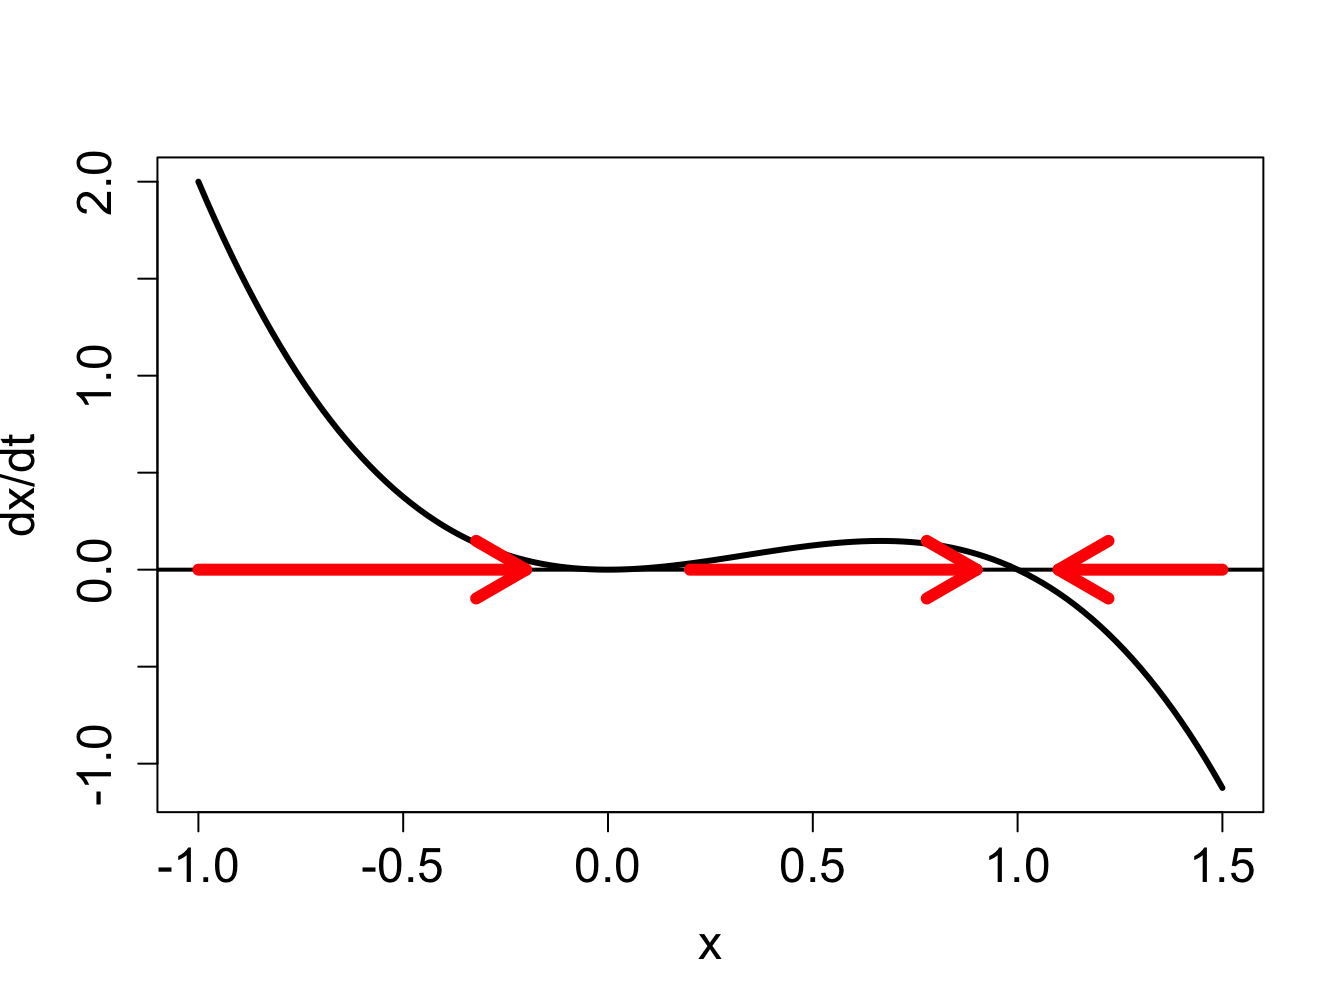
\includegraphics[width=0.5\linewidth]{QuantLife_files/figure-latex/ch7-flow3-1} 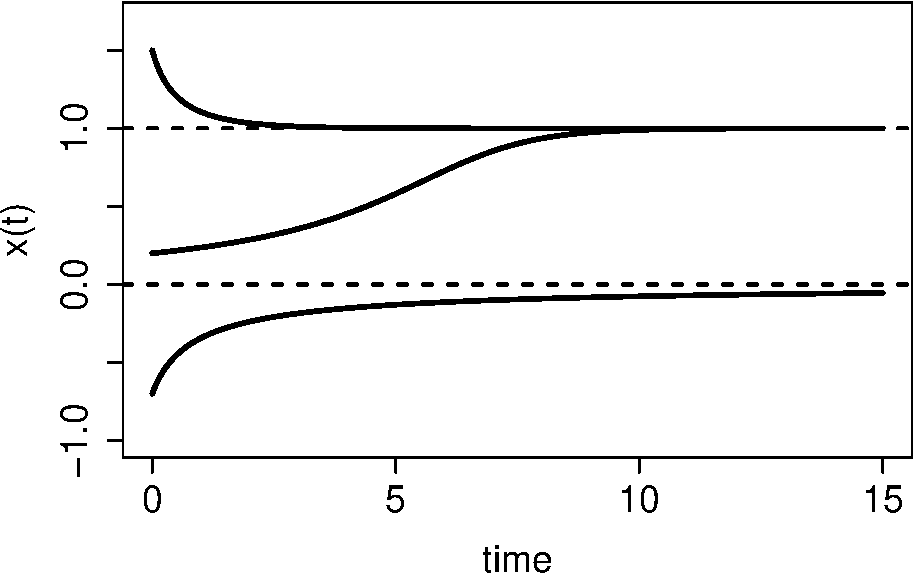
\includegraphics[width=0.5\linewidth]{QuantLife_files/figure-latex/ch7-flow3-2} 

}

\caption{a) plot of the defining function of the ODE $dx/dt = -x^3 + x^2$ with direction of flow of x(t) indicated with arrows on the x-axis; b) plot of solutions x(t) of the ODE staring with three initial values}\label{fig:ch7-flow3}
\end{figure}

\hypertarget{exercises-19}{%
\subsection{Exercises}\label{exercises-19}}

For the following differential equations: a) plot the defining function over the indicated range (use any computational tools you wish) to determine the intervals on which the dependent variable is increasing and decreasing; b) find the equilibria c) determine the stability of each equilibrium; d) based on your analysis in parts a-c, sketch (by hand) plots of the solutions with the specified initial values.

\begin{enumerate}
\def\labelenumi{\arabic{enumi}.}
\item
  \[ \frac{dC}{dt} = -0.2C + 60; \; C \in (0,500); \; C(0) = 200; \; C(0) = 400 \]
\item
  \[ \frac{dP}{dt} = 0.01P(800-P) - 0.5P; \; P \in (-1, 1000); \; P(0) = 100; \; P(0) = 800\]
\item
  \[ \frac{dR}{dt} = R(80-R) - 1200; \; R \in (-1, 100); \; R(0) = 10; \; R(0) = 80\]
\item
  \[ \frac{dI}{dt} = 0.1I(1-I) - 0.03I; \;  I \in (-0.1, 1.1); \; I(0) = 0.2; \; I(0) = 0.9 \]
\item
  \[  \frac{dR}{dt} = \frac{R}{1+R}-0.1R; \; R \in (-0.1, 10); \; R(0) = 20; \; R(0) = 0 \]
\item
  \[  \frac{dP}{dt} =  0.02P(P-100)(1200-P) \; P \in (-0.1, 1200); \; P(0) = 20; \; P(0) = 1000 \]
\item
  \[  \frac{dY}{dt} =  0.01Y(Y-100)(Y-200) \; Y \in (-0.1, 300); \; Y(0) = 20; \; Y(0) = 250 \]
\item
  (harder) The logistic function \index{logistic model}\index{function!logistic}was defined in chapter 2, equation 2.4. Verify that the logistic function with independent variable \(t\) solves the logistic ODE in equation \ref{eq:log_cont_model} and relate the parameters in the function to the parameters \(r\) and \(K\) in the ODE.
\end{enumerate}

\hypertarget{functions-in-r}{%
\section{Functions in R}\label{functions-in-r}}

Like most programming languages, R allows one to define and use structures called \index{function!in R}\index{R programming!function}functions. Some are already written and loaded into the R distribution, for example, the function \texttt{mean()} we use to compute the mean of a vector variable, while others can be defined by users. Functions are discrete chunks of code that can be \emph{called} from the outside to perform some task. The function receives inputs from the call and returns the result back. Here is the general structure of a function in R:

\begin{Shaded}
\begin{Highlighting}[]
\NormalTok{myfunction \textless{}{-}}\StringTok{ }\ControlFlowTok{function}\NormalTok{(arg1, arg2, ...) \{}
\NormalTok{    statements}
    \KeywordTok{return}\NormalTok{(answer)}
\NormalTok{\}}
\end{Highlighting}
\end{Shaded}

A function is a piece of code that is \textbf{defined} separately and can be \textbf{called} by other pieces of code. The main purpose is to create a ``black box'' that does a specific job and can be used repeatedly just by calling the function (invoking its name), rather than copying the code repeatedly.

A function generally has input variables (although sometimes there are none) and returns an output using the \texttt{return()} statement. It is important to distinguish between the \emph{inside} of the function - the code between the curly braces in the function definition - and the \emph{outside}, that is everything else. The inputs are \emph{passed} to the function in the call (through the parentheses) and then used inside the function to do its business and produce an output, which is then \emph{returned} back to the place in the code where the function was called.

\hypertarget{defining-a-function}{%
\subsection{defining a function}\label{defining-a-function}}

Here is an example of a function definition, with input variables N and r. Between the curly braces is the \emph{body of the function}, which in this case multiplies the two input variables and then returns them.

\begin{Shaded}
\begin{Highlighting}[]
\NormalTok{my\_funk \textless{}{-}}\StringTok{ }\ControlFlowTok{function}\NormalTok{(N,r)\{ }
\NormalTok{  ans \textless{}{-}}\StringTok{ }\NormalTok{r}\OperatorTok{*}\NormalTok{N }\CommentTok{\# updating function f(N)}
  \KeywordTok{return}\NormalTok{(ans)}
\NormalTok{\}}
\end{Highlighting}
\end{Shaded}

Note that after running the code chunk above, you should see the name \texttt{my\_funk} in your environment (under Functions). This means this function is defined in memory and ready to be called.

\hypertarget{calling-a-function}{%
\subsection{calling a function}\label{calling-a-function}}

After a function is defined, it is ready to be called (executed) by invoking its name and giving the correct number of inputs. Here's an example of a function call:

\begin{Shaded}
\begin{Highlighting}[]
\NormalTok{a \textless{}{-}}\StringTok{ }\DecValTok{30}
\NormalTok{y \textless{}{-}}\StringTok{ }\DecValTok{1}\OperatorTok{:}\DecValTok{10}
\KeywordTok{print}\NormalTok{(}\KeywordTok{my\_funk}\NormalTok{(y, a))}
\end{Highlighting}
\end{Shaded}

\begin{verbatim}
##  [1]  30  60  90 120 150 180 210 240 270 300
\end{verbatim}

Notice that the variable names in the fuction call do not have to be same as what they are called within the function. IMPORTANT: a function uses the order of variables in the function call, called \emph{external variables} (\texttt{y}, \texttt{a}) to assign their names within the function, called \emph{internal variables} (\texttt{N}, \texttt{r}). (There is a way to specify which input belongs to which internal variable, e.g.~\texttt{plot(x=time,\ y=sol)} and in that case the order is not important.)

\hypertarget{using-a-function-to-solve-a-difference-equation}{%
\subsection{using a function to solve a difference equation}\label{using-a-function-to-solve-a-difference-equation}}

We have solved discrete-time dynamic models (difference equations) using for loops. You can use a function to calculate the next value of the solution, by passing the current value and any parameters as inputs to the function, as you can see in the code chunk below:

\begin{Shaded}
\begin{Highlighting}[]
\NormalTok{numsteps\textless{}{-}}\DecValTok{30} \CommentTok{\# set number of steps}
\NormalTok{sol \textless{}{-}}\StringTok{ }\KeywordTok{rep}\NormalTok{(}\DecValTok{0}\NormalTok{,numsteps}\OperatorTok{+}\DecValTok{1}\NormalTok{) }\CommentTok{\# pre{-}allocate sol1}
\NormalTok{sol[}\DecValTok{1}\NormalTok{] \textless{}{-}}\StringTok{ }\DecValTok{100} \CommentTok{\# set initial value}
\NormalTok{r \textless{}{-}}\StringTok{ }\DecValTok{2} \CommentTok{\# define the multiplicative constant}
\ControlFlowTok{for}\NormalTok{ (i }\ControlFlowTok{in} \DecValTok{1}\OperatorTok{:}\NormalTok{numsteps) \{ }\CommentTok{\# repeat for numsteps}
\NormalTok{  sol[i}\OperatorTok{+}\DecValTok{1}\NormalTok{] \textless{}{-}}\StringTok{ }\KeywordTok{my\_funk}\NormalTok{(sol[i], r) }\CommentTok{\# calculate the next value}
\NormalTok{\}}
\NormalTok{time \textless{}{-}}\StringTok{ }\DecValTok{0}\OperatorTok{:}\NormalTok{numsteps }\CommentTok{\# define time vector}
\KeywordTok{plot}\NormalTok{(time,sol,}\DataTypeTok{t=}\StringTok{\textquotesingle{}b\textquotesingle{}}\NormalTok{,}\DataTypeTok{xlab=}\StringTok{\textquotesingle{}time\textquotesingle{}}\NormalTok{,}\DataTypeTok{ylab=}\StringTok{\textquotesingle{}solution\textquotesingle{}}\NormalTok{,}\DataTypeTok{lwd=}\DecValTok{2}\NormalTok{)}
\end{Highlighting}
\end{Shaded}

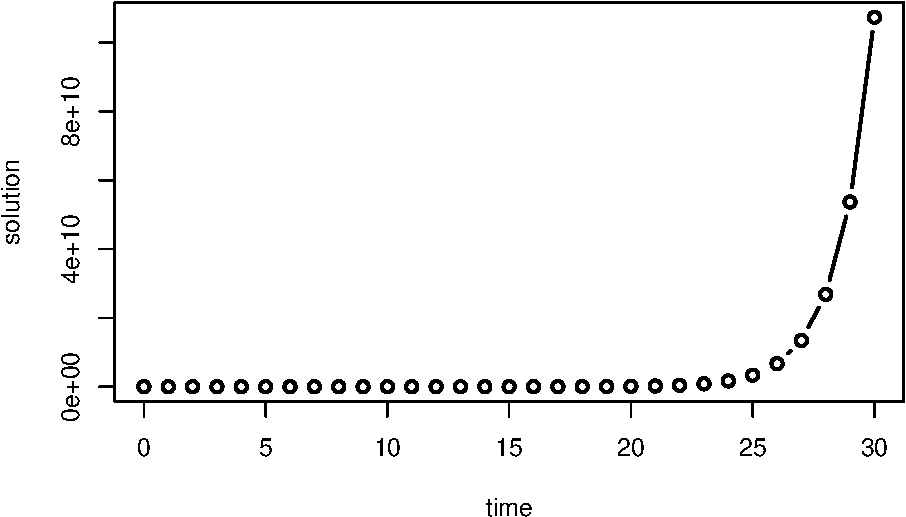
\includegraphics{QuantLife_files/figure-latex/unnamed-chunk-126-1.pdf}

\hypertarget{exercises-20}{%
\subsection{Exercises}\label{exercises-20}}

\begin{enumerate}
\def\labelenumi{\arabic{enumi}.}
\tightlist
\item
  Write a function that takes the input variable and multiplies it by 1.03, like the mathematical function \(f(x) = 1.03x\).
\end{enumerate}

\begin{Shaded}
\begin{Highlighting}[]
\CommentTok{\# YOUR CODE HERE}
\end{Highlighting}
\end{Shaded}

\begin{enumerate}
\def\labelenumi{\arabic{enumi}.}
\setcounter{enumi}{1}
\tightlist
\item
  Use the function to take a variable and multiply it by 1.03, replacing the old value of the variable. If the initial value is 5, the new value should be 5.15.
\end{enumerate}

\begin{Shaded}
\begin{Highlighting}[]
\CommentTok{\# YOUR CODE HERE}
\end{Highlighting}
\end{Shaded}

\begin{enumerate}
\def\labelenumi{\arabic{enumi}.}
\setcounter{enumi}{2}
\tightlist
\item
  Write a script to take a variable and multiply it by 1.03 one hundred times, replacing the old value of the variable \textbf{using a for loop and the function you created}. Starting with the initial value is 5, the script should return the value 96.093.
\end{enumerate}

\begin{Shaded}
\begin{Highlighting}[]
\CommentTok{\# YOUR CODE HERE}
\end{Highlighting}
\end{Shaded}

\begin{enumerate}
\def\labelenumi{\arabic{enumi}.}
\setcounter{enumi}{3}
\tightlist
\item
  Modify the script above to save all the intermediate values into a vector, and plot a graph of this vector vs.~the iteration step (from 1 to 101). Hint: this is exactly like the example code above.
\end{enumerate}

\begin{Shaded}
\begin{Highlighting}[]
\CommentTok{\# YOUR CODE HERE}
\end{Highlighting}
\end{Shaded}

\hypertarget{modeling-the-spread-of-infectious-disease-spread}{%
\section{Modeling the spread of infectious disease spread}\label{modeling-the-spread-of-infectious-disease-spread}}

\label{sec:bio16}

The field of \emph{epidemiology} studies the distribution of disease and health states in populations. Epidemiologists describe and model these issues with the goal of helping public health workers devise interventions to improve the overall health outcomes on a large scale. One particular topic of interest is the the spread of infectious disease and how best tor respond to it.. Because epidemiology is concerned with large numbers of people, the models used in the field do not address the details of an individual disease history. One approach to modeling this is to put people into categories, such as \emph{susceptible} (those who can be infected but are not), \emph{infectious} (those who are infected and can spread the disease), and \emph{recovered} (those who cannot be infected or spread disease). This type of models is called a \index{epidemic!compartment model} \emph{compartment model} and they are they commonly used to represent infectious disease on a population level both for deterministic models (e.g.~ODEs) and stochastic models (e.g.~Markov models). Dividing people into categories involves the assumption that everyone in a particular category behaves in the same manner: for instance, all susceptible people are infected with the same rate and all infected people recover with the same rate.

Let us construct an ODE to describe a two-compartment epidemiology model. There are two dependent variables to be tracked: the number of susceptible (\(S\)) and infected (\(I\)) individuals in the population. The susceptible individuals can get infected, while the infected ones can recover and become susceptible again. The implicit assumption is that there is no immunity, and recovered individuals can get infected with the same ease as those who were never infected. There are some human diseases for which this is true, for instance the common cold or gonorrhea. Transitions between the different classes of individuals can be summarized by the following scheme:
\[ S + I \xrightarrow{\beta} I \xrightarrow{\gamma} S \]
Here \(\beta\) is the individual rate of infection, also known as the transmission rate, and \(\gamma\) is the individual rate of recovery. There is an important distinction between the processes of infection and recovery: the former requires an infected individual and a susceptible individual, while the latter needs only an infected individual. Therefore, it is reasonable to suppose that the rate of growth of infected individuals is the product of the individual transmission rate \(\beta\) and the product of the number of infected and susceptible individuals. The overall rate of recovery is the individual recovery rate \(\gamma\) multiplied by the number of the infected. This leads to the following two differential equations:
\begin{eqnarray*}
\dot S &=& -\beta IS + \gamma I \\
\dot I & = &\beta I S - \gamma I
\end{eqnarray*}
Note that, as in the chemical kinetics models, the two equations add up to zero on the right hand side, leading to the conclusion that \(\dot S + \dot I = 0\). Therefore, the total number of people is a conserved quantity \(N\), which does not change. This makes sense since we did not consider any births or deaths in the ODE model, only transitions between susceptible and infected individuals.

We can use the conserved quantity \(N\) to reduce the two equations to one, by the substitution of \(S = N -I\):
\[  \dot I  =  \beta I (N - I) - \gamma I \]
This model may be analyzed using qualitative methods that were developed in this chapter, allowing prediction of the dynamics of the fraction of infected for different transmission and recovery rates. First, let us find the fixed points of the differential equation. Setting the equation to zero, we find:
\[ 0  =  \beta I (N - I) - \gamma I \Rightarrow I^* = 0; \; I^* =  N - \gamma/\beta \]
This means that there are two equilibrium levels of infection: either nobody is infected (\(I^* = 0\)) or there is some persistent number of infected individuals (\$ I\^{}* = N - \gamma/\beta \$). Notice that the second fixed point is only biologically relevant if \$N \textgreater{} \gamma/\beta \$.

Use the derivative test to check for stability. First, find the general expression for derivative of the defining function: \$f'(I) = -2 \beta I + \beta N - \gamma \$.
\textbackslash begin\{figure\}{[}htbp{]} \% figure placement: here, top, bottom, or page

\begin{figure}

{\centering 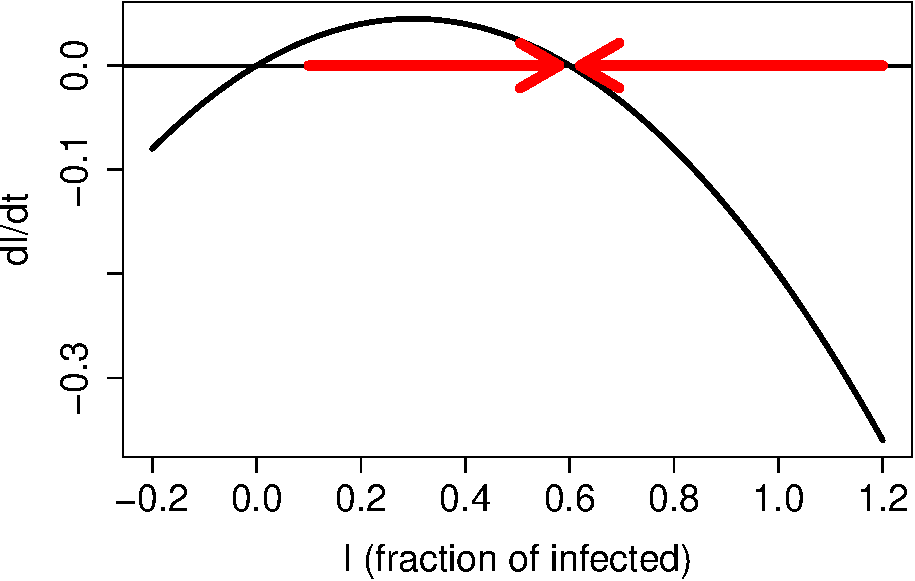
\includegraphics[width=0.5\linewidth]{QuantLife_files/figure-latex/ch7-flow-sis1-1} 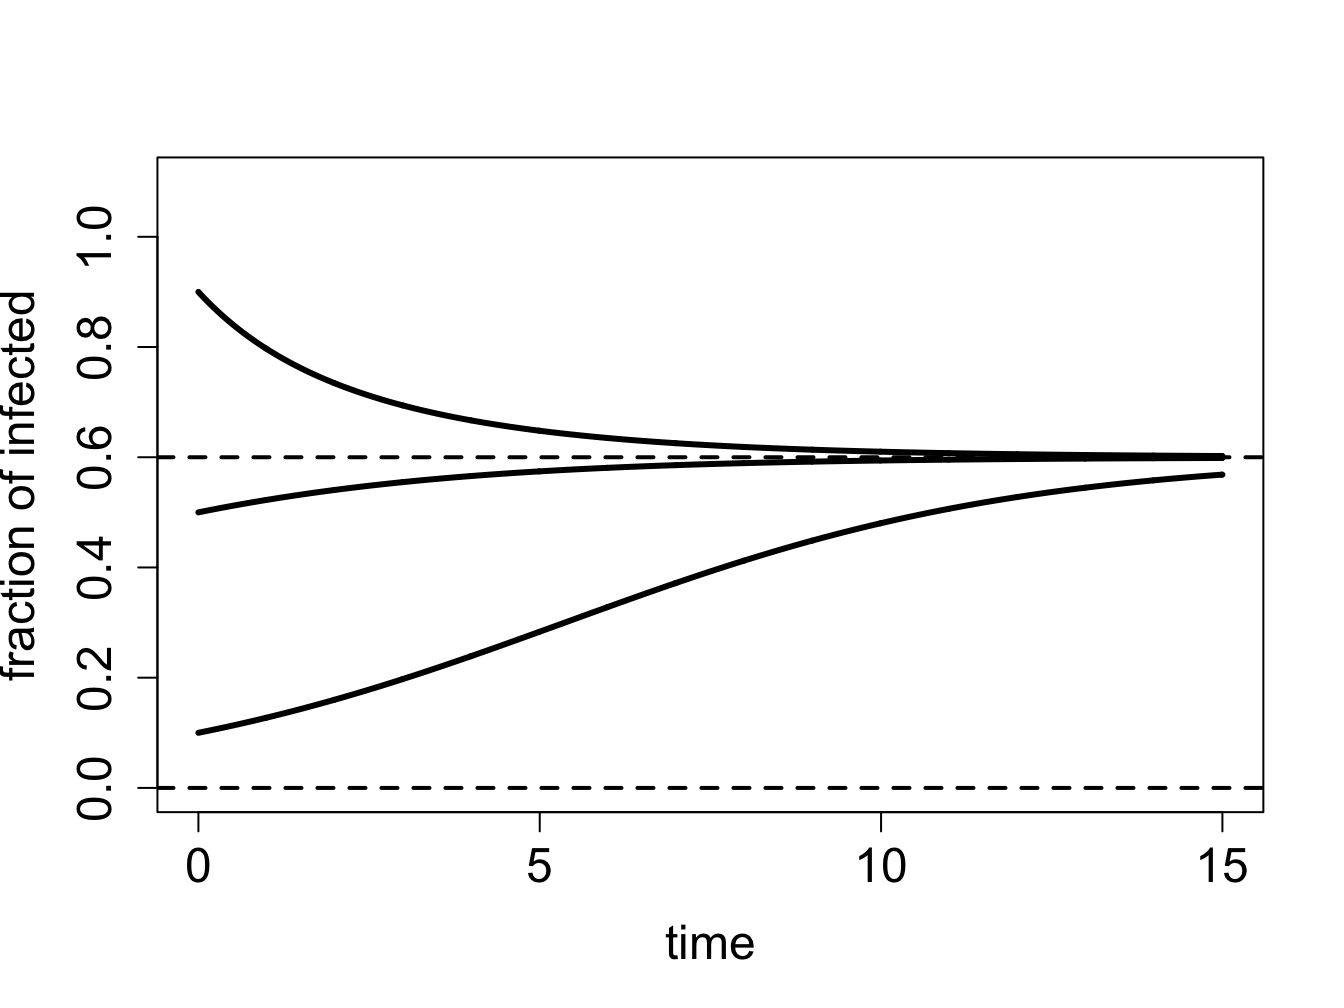
\includegraphics[width=0.5\linewidth]{QuantLife_files/figure-latex/ch7-flow-sis1-2} 

}

\caption{Graphical analysis of the SIS model with $I$ representing the fraction of infected individuals (N=1) and beta=0.5 and gamma = 0.2; a) plot showing the flow of the solutions on the I-axis, with a stable equilibrium at 0.6 and an unstable equilibrium at 0; b) three solutions of the model starting at three different initial values all converge to the same fraction of infected.}\label{fig:ch7-flow-sis1}
\end{figure}

\begin{figure}

{\centering \includegraphics[width=0.5\linewidth]{QuantLife_files/figure-latex/ch7-flow-sis2-1} \includegraphics[width=0.5\linewidth]{QuantLife_files/figure-latex/ch7-flow-sis2-2} 

}

\caption{Graphical analysis of the SIS model with I representing the fraction of infected individuals (N=1) and beta=0.2 and gamma = 0.3; a) plot showing the flow of the solutions on the I-axis, with a stable equilibrium at 0 and an unstable equilibrium at -0.5; b) three solutions of the model starting at three different initial values all converge to 0 infected.}\label{fig:ch7-flow-sis2}
\end{figure}

The stability of the fixed point \(I^* = 0\) is found by plugging in this value into the derivative formula: \$f'(0) = \beta N - \gamma \$. We learned in section \ref{sec:math16} that a fixed point is stable if the derivative of the defining function is negative. Therefore, \(I^* = 0\) is stable if \(\gamma - \beta N > 0\), and unstable otherwise. This gives us a \index{differential equation!stability condition} \emph{stability condition} on the values of the biological parameters. If the recovery rate \(\gamma\) is greater than the rate of infection for the population (the transmission rate multiplied by the population size) \(\beta N\), then the no-infection equilibrium is stable. This predicts that the infection dies out if the recovery rate is faster than the rate of infection, which makes biological sense.

Similarly, we find the stability of the second fixed point \(I^* = N - \gamma/\beta\) by substituting its value into the derivative, to obtain \(f'(N - \gamma/\beta) = \gamma - \beta N\). By the same logic, as above, this fixed point is stable if \(\gamma - \beta N < 0\), or if \(\gamma < \beta N\). This is a complementary condition for the fixed point at 0, that is, only one fixed point can be stable for any given parameter values. In the biological interpretation, if the transmission rate \(\beta N\) is greater than the recovery rate \(\gamma\), then the epidemic will persist.

We can use our graphical analysis skills to illustrate the situation. Consider a situation in which \(\gamma < \beta N\). As predicted by stability analysis, the zero infection equilibrium should be unstable, and the equilibrium at \(N - \gamma/\beta\) should be stable. In order to plot the function \$f(I) = \beta I (N - I) - \gamma I \$, we choose the specific parameter values \(N=1\), \(\gamma = 0.1\) and \(\beta = 0.2\); setting \(N=1\) means \(S\) and \(I\) represent the fraction of the population in the susceptible and infected categories. Figure \ref{fig:ch16_flow_sis1}a shows the direction of the flow on the \(I\)-axis prescribed by the defining function \(f(I)\) with red arrows. It is clear that solutions approach the fixed point at \(N - \gamma/\beta\) from both directions, which make it a stable fixed point, while diverging from \(I=0\), as shown in figure \ref{fig:ch16_flow_sis1}b.

On the other hand, if \(\gamma > \beta N\), stability analysis predicts that the no-infection equilibrium (\(I=0\)) is stable. Figure \ref{fig:ch16_flow_sis2}a shows the plot of the defining function for the parameter values \(N=1\), \(\gamma = 0.3\) and \(\beta = 0.2\). The flow on the \(I\)-axis is toward the zero equilibrium, therefore it is stable. Note that the second equilibrium at \(I^* = N - \gamma/\beta\) is negative, and thus has no biological significance. The solutions, if the initial value is positive, all approach 0, so the infection inevitably dies out.

Mathematical modeling of epidemiology has been a success story in the last few decades. Public health workers routinely estimate the \index{parameter!basic reproductive number}parameter called the \index{epidemic!basic reproductive number} \emph{basic reproductive number} \(R_0\) defined to be the average number of new infections caused by a single infected individual in a susceptible population. This number comes out of our analysis above, where we found \(R_0 = N \beta/\gamma\) to determine whether or not an epidemic persisted \citep{brauer_mathematical_2011}. This number is critical in more sophisticated models of epidemiology.

Mathematical models are used to predict the time course of an epidemic, called the \index{epidemic!curve} \emph{epidemic curve} and then advise on the public health interventions that can reduce the number of affected individuals. In reality, most epidemic curves have the shape similar to the data from the Ebola virus epidemic in figure \ref{fig:ch16-ebola}. Most such curves show an initial increase in infections, peaking, and the declining to low levels, which is fundamentally different than the solution curves we obtained from the two-compartment model. To describe dynamics of this nature, models with more than two variables are needed, such as classic three-compartment SIR models (susceptible-infected-recovered) models and their modifications \citep{brauer_mathematical_2011}. Being able to predict the future of an epidemic based on \(R_0\) and other parameters allows public health officials to prepare and deploy interventions (vaccinations, quarantine, etc.) that have the best shot at minimizing the epidemic.

\begin{figure}

{\centering \includegraphics[width=0.5\linewidth]{QuantLife_files/figure-latex/ch7-ebola-1} \includegraphics[width=0.5\linewidth]{QuantLife_files/figure-latex/ch7-ebola-2} 

}

\caption{Number of new cases of ebola virus infections  per week in Liberia (left) and Sierra Leone (right), time ranging from March 17, 2014 (week 1) until May 20, 2015 (week 61). Data from http://apps.who.int/gho/data/node.ebola-sitrep.}\label{fig:ch7-ebola}
\end{figure}

\hypertarget{discussion}{%
\subsection{Discussion}\label{discussion}}

The following questions encourage you to think critically about modeling of infectious diseases.

\begin{enumerate}
\def\labelenumi{\arabic{enumi}.}
\item
  What effect does changing the infection rate \(\beta\) have on the basic reproductive rate? Explain the biological intuition behind this.\}
\item
  What effect does changing the recovery rate \(\gamma\) have on the basic reproductive rate? Explain the biological intuition behind this.\}
\item
  Discuss what assumptions are made by using compartment models, and when they might be justified.\}
\item
  Discuss the difference in assumptions in using a Markov model with Susceptible and Infected compartments compared to an ODE model with the same two compartments. Under what circumstances does it make sense to use one or the other?\}
\item
  Read the paper \citep{agusto_mathematical_2015} and discuss the strengths and limitations of the more complicated compartment model intended to account for human behavior.\}
\end{enumerate}

\hypertarget{r-assignment-6}{%
\section{R Assignment}\label{r-assignment-6}}

\begin{Shaded}
\begin{Highlighting}[]
\CommentTok{\# Define the function:}
\NormalTok{DefFunk \textless{}{-}}\StringTok{ }\ControlFlowTok{function}\NormalTok{ (x,a,b)\{}
\NormalTok{  ans \textless{}{-}}\StringTok{ }\NormalTok{a}\OperatorTok{*}\NormalTok{x}\OperatorTok{\^{}}\DecValTok{2}\OperatorTok{{-}}\NormalTok{b}
  \KeywordTok{return}\NormalTok{(ans)}
\NormalTok{\}  }
\NormalTok{a \textless{}{-}}\StringTok{ }\DecValTok{1}
\NormalTok{b \textless{}{-}}\StringTok{ }\DecValTok{4}
\NormalTok{x\textless{}{-}}\KeywordTok{seq}\NormalTok{(}\OperatorTok{{-}}\DecValTok{5}\NormalTok{,}\DecValTok{5}\NormalTok{,}\FloatTok{0.1}\NormalTok{) }\CommentTok{\# define the array of values of x}
\NormalTok{y\textless{}{-}}\KeywordTok{DefFunk}\NormalTok{(x,a,b) }\CommentTok{\# calculate the values of y using a function}
\KeywordTok{plot}\NormalTok{(x,y,}\DataTypeTok{t=}\StringTok{"l"}\NormalTok{,}\DataTypeTok{xlab=}\StringTok{"x"}\NormalTok{, }\DataTypeTok{ylab=}\StringTok{"dx/dt"}\NormalTok{) }\CommentTok{\# plot the function}
\KeywordTok{abline}\NormalTok{(}\DecValTok{0}\NormalTok{,}\DecValTok{0}\NormalTok{) }\CommentTok{\# draw a line for y=0}
\end{Highlighting}
\end{Shaded}

\includegraphics{QuantLife_files/figure-latex/unnamed-chunk-131-1.pdf}

Notice that I used two input variables into the defining function (a and b) as parameters that can be changed \emph{outside} the function. This is good coding practice - the best way to use a function is by changing its inputs, not monkeying with its internal code.

After qualitative analysis, you will check whether solutions behave in the predicted way by running Forward Euler to calculate the numerical solution.

\hypertarget{logistic-population-model}{%
\subsection{logistic population model}\label{logistic-population-model}}

This is the logistic model of population growth, with P representing population size, r is the growth rate parameter, and K is the carrying capacity parameter; P is measured in thousands, and time is measured in years.
\[ \frac{dP}{dt} = rP(1-P/K) \]

\begin{enumerate}
\def\labelenumi{\arabic{enumi}.}
\item
  \begin{enumerate}
  \def\labelenumii{\alph{enumii})}
  \tightlist
  \item
    For the values of r=0.3 and K=40, plot the graph of the defining function (right-hand side of the ODE) in R over some interval that includes all zeros of the function. Based on the graph, find the equilibria of the ODE, determine their stability, and predict the behavior of the solution for the following initial values: P(0) = 1; P(0) = 39; P(0) = 20.
  \end{enumerate}
\end{enumerate}

\begin{Shaded}
\begin{Highlighting}[]
\CommentTok{\#YOUR CODE HERE}
\end{Highlighting}
\end{Shaded}

YOUR ANSWERS HERE

\begin{enumerate}
\def\labelenumi{\alph{enumi})}
\setcounter{enumi}{1}
\tightlist
\item
  Uses the Forward Euler method to calculate the numeric solution of the logistic ODE for any given values of r and K (they should be inputs into your defining function). Use this script to solve the logistic ODE with parameters r=0.3 and K=40, with a small time step (e.g.~dt=0.1) and the following initial values: P(0) = 1; P(0) = 39; P(0) = 20. Calculate the numerical solutions of the ODE over a sufficiently large time Tmax to observe convergence, and plot all three in the same figure. Do the solution plots look consistent with your prediction in question a?
\end{enumerate}

\begin{Shaded}
\begin{Highlighting}[]
\CommentTok{\#YOUR CODE HERE}
\end{Highlighting}
\end{Shaded}

YOUR ANSWERS HERE

\begin{enumerate}
\def\labelenumi{\arabic{enumi}.}
\setcounter{enumi}{1}
\tightlist
\item
  For the values of the parameters r=0.02 and K=120, plot the graph of the defining function (right-hand side of the ODE) in R over some interval that includes all zeros of the function. Based on the graph, find the equilibria of the ODE, determine their stability, and predict the behavior of the solution for the following initial values: P(0) = 10; P(0) = 50; P(0) = 150.
\end{enumerate}

\begin{Shaded}
\begin{Highlighting}[]
\CommentTok{\#YOUR CODE HERE}
\end{Highlighting}
\end{Shaded}

YOUR ANSWERS HERE

\begin{enumerate}
\def\labelenumi{\alph{enumi})}
\setcounter{enumi}{1}
\tightlist
\item
  Use the Forward Euler method to calculate the numeric solution of the logistic ODE with parameters r=0.02 and K=120 with a small time step (e.g.~dt=0.1) and the following initial values: P(0) = 10; P(0) = 50; P(0) = 150. Plot the numeric solutions of the ODE over a sufficiently large time Tmax to observe convergence. Do the solution plots look consistent with your prediction in question a?
\end{enumerate}

\begin{Shaded}
\begin{Highlighting}[]
\CommentTok{\#YOUR CODE HERE}
\end{Highlighting}
\end{Shaded}

YOUR ANSWERS HERE

\begin{enumerate}
\def\labelenumi{\arabic{enumi}.}
\setcounter{enumi}{2}
\tightlist
\item
  Let r=0.3 and K=40 and start at P(0)=1. Gradually increase dt until you see the solution behaving differently than expected. Report at what value of dt this strange behavior begins, investigate what happens for even larger time steps, and describe what happens to the solutions.
\end{enumerate}

\begin{Shaded}
\begin{Highlighting}[]
\CommentTok{\#YOUR CODE HERE}
\end{Highlighting}
\end{Shaded}

YOUR ANSWERS HERE

\hypertarget{sis-model-of-infectious-disease}{%
\subsection{SIS model of infectious disease}\label{sis-model-of-infectious-disease}}

The following ODE is a simple model of an infectious epidemic with only two kinds of individuals: susceptible and infected, and where the total population size stays the same. The variable I is the fraction of individuals in the population who are infected, and the parameters beta and gamma are the infection and recovery rates, respectively; time is measured in days.
\[ \frac{dI}{dt} = \beta I(1-I) - \gamma I \]

\begin{enumerate}
\def\labelenumi{\arabic{enumi}.}
\item
  \begin{enumerate}
  \def\labelenumii{\alph{enumii})}
  \tightlist
  \item
    For the values of beta = 0.4 and gamma=0.1 plot the graph of the defining function (right-hand side of the ODE) in R over the interval {[}0,1{]}. Based on the graph, find the equilibria of the ODE, determine their stability, and predict the behavior of the solution for the following initial values: I(0) = 0.01; I(0) = 0.8; I(0) = 0.5.
  \end{enumerate}
\end{enumerate}

\begin{Shaded}
\begin{Highlighting}[]
\CommentTok{\#YOUR CODE HERE}
\end{Highlighting}
\end{Shaded}

YOUR ANSWERS HERE

\begin{enumerate}
\def\labelenumi{\alph{enumi})}
\setcounter{enumi}{1}
\tightlist
\item
  Write a Forward Euler script to calculate the numeric solution of the SIS model ODE for any given values of beta and gamma (they should be inputs into your defining function). Use this script to solve the SIS model ODE with parameters beta = 0.4 and gamma=0.1 , with a small time step (e.g.~dt=0.1) and the following initial values: I(0) = 0.01, I(0) = 0.5, I(0) = 0.9. Plot the numerical solutions of the ODE over a sufficiently large time Tmax to observe convergence. Report whether the epidemic persists or burns out, whether it depends on the initial value, and comment on whether the solution dynamics agrees with your prediction in question a).
\end{enumerate}

\begin{Shaded}
\begin{Highlighting}[]
\CommentTok{\#YOUR CODE HERE}
\end{Highlighting}
\end{Shaded}

YOUR ANSWERS HERE

\begin{enumerate}
\def\labelenumi{\arabic{enumi}.}
\setcounter{enumi}{1}
\item
  \begin{enumerate}
  \def\labelenumii{\alph{enumii})}
  \tightlist
  \item
    For the values of beta=0.1 and gamma=0.2 plot the graph of the defining function (right-hand side of the ODE) in R over the interval {[}0,1{]}. Based on the graph, find the equilibria of the ODE, determine their stability, and predict the behavior of the solution for the following initial values: I(0) = 0.01; I(0) = 0.5; I(0) = 0.8.
  \end{enumerate}
\end{enumerate}

\begin{Shaded}
\begin{Highlighting}[]
\CommentTok{\#YOUR CODE HERE}
\end{Highlighting}
\end{Shaded}

YOUR ANSWERS HERE

\begin{enumerate}
\def\labelenumi{\alph{enumi})}
\setcounter{enumi}{1}
\tightlist
\item
  Use the Forward Euler script to solve the SIS model ODE with parameters beta=0.1 and gamma=0.2 with a small time step (e.g.~dt=0.1) and the following initial values: I(0) = 0.01; I(0) = 0.8; I(0) = 0.5. Plot the numerical solutions of the ODE over a sufficiently large time Tmax to observe convergence. Report whether the epidemic persists or burns out (converges to zero), how it depends on the initial value, and comment on whether the solution dynamics agrees with your prediction in question a.
\end{enumerate}

\begin{Shaded}
\begin{Highlighting}[]
\CommentTok{\#YOUR CODE HERE}
\end{Highlighting}
\end{Shaded}

YOUR ANSWERS HERE

\begin{enumerate}
\def\labelenumi{\arabic{enumi}.}
\setcounter{enumi}{2}
\tightlist
\item
  For I(0)=0.5 and beta=0.1, starting with gamma=0.3, progressively decrease the value of the recovery rate gamma, and report the behavior of the numerical solution (with a small enough dt and a large enough Tmax so you can see the asymptotic behavior). Report the critical value of gamma at which the fraction of infected converges to a positive equilibrium value (the disease does not burn out.) Keep decreasing the recovery rate and report what happens to the equilibrium fraction of infected people. Does it ever get to 1?
\end{enumerate}

\begin{Shaded}
\begin{Highlighting}[]
\CommentTok{\#YOUR CODE HERE}
\end{Highlighting}
\end{Shaded}

YOUR ANSWERS HERE

\hypertarget{part-randomness-in-observations}{%
\part{Randomness in observations}\label{part-randomness-in-observations}}

\hypertarget{random-variables-and-distributions}{%
\chapter{Random variables and distributions}\label{random-variables-and-distributions}}

\begin{quote}
What is there then that can be taken as true? Perhaps only this one thing, that nothing at all is certain.
-- Rene Descartes
\end{quote}

Mathematical models can be divided into \emph{deterministic} and \emph{stochastic} models. Deterministic models assume that the future can be perfectly predicted based on complete information of the past. Stochastic models instead assume that even perfect knowledge of the past does not allow one to predict the future with certainty.

Stochastic models may not sound very promising: after all, we want to make predictions, and randomness says that predictions are impossible! However, the word ``random'' in mathematics doesn't mean ``completely unpredictable'' or ``without rules,'' as it does in common usage. It means that we can make probabilistic predictions, e.g.~compute what fraction of molecules will diffuse from one place to another, or what fraction of genes mutate in one generation - we just can't make a definite prediction for each individual molecule or gene. Biological processes are so complex and are subject to so much environmental noise, that stochastic models are absolutely essential for our understanding of many living systems. Here is what you will learn to do in this chapter:

\begin{itemize}
\item
  define probability in terms of outcomes and events
\item
  know what is a random variable and its distribution
\item
  compute means and variances of distributions
\item
  use the binomial distribution to model strings of binary trials
\item
  generate random numbers in R
\end{itemize}

\hypertarget{random-variables-and-distributions-1}{%
\section{Random variables and distributions}\label{random-variables-and-distributions-1}}

\label{sec:math4_1}

\hypertarget{definition-of-probability}{%
\subsection{definition of probability}\label{definition-of-probability}}

In this section we will develop the terminology used in the mathematical study of randomness called probability. This begins with a \emph{random experiment} which is a very broad term that can describe any natural or theoretical process whose outcome cannot be predicted with certainty. If the outcomes are numeric, they may be \emph{discrete} (can be counted by integers) or \emph{continuous} (corresponding to real numbers); they may also be \emph{categorical}, meaning that they do not have a numeric meaning, like eye color. We will stick to experiments that have discrete outcomes in this chapter, but many important experiments produce continuous outcomes. The first step for studying a random process is to describe all of the outcomes it can produce:

\begin{definition}
\protect\hypertarget{def:def-sampspace}{}{\label{def:def-sampspace} }The collection of all possible outcomes of an experiment is called its \emph{sample space} \(\Omega\). An \emph{event} is a subset of the sample space, which means an event may contain one or more experimental outcomes.
\end{definition}

\begin{figure}
\centering
\includegraphics{ch4/sample_space.png}
\caption{An illustration of the sample space of all people with two events: tall people and those who like tea.}
\end{figure}

\textbf{Example.} You can ask a person two questions: how tall are you (and classify them either as short or tall) and do you like tea (yes or no), and you've performed a random experiment. The randomness comes not from the answers (assuming the person doesn't randomly lie) but from the selection of the respondent. We will discuss randomly selecting a sample from a population in the next chapter. This random experiment has four outcomes: tall person who likes tea, tall person who does not like tea, short person who likes tea, and short person who does not like tea. This sample space and events is illustrated in figure \ref{fig:ch4_sample_space} with a Venn diagram, which uses geometric shapes as representations of events as subsets of the entire sample space. These outcomes can be grouped into events by one of the responses: e.g.~tall person (\(A\)) or person who doesn't like tea (\(-B\)).

\textbf{Example.} A random experiment with two outcomes, called a \emph{Bernoulli trial} (after the famous Swiss mathematician), can describe a variety of situations: a coin toss (heads or tails), a competition with two outcomes (win or loss), the allele of a gene (normal or mutant). The sample space for a single Bernoulli trial consists of just two outcomes: \(\{H,T\}\) (for a coin toss). If the experiment is performed repeatedly, the sample space gets more complicated. For two Bernoulli trials there are four different outcomes \(\{HH, HT, TH, TT \}\). One can define different events for this sample space: the event of getting two heads in two tosses contains one outcome: \(\{HH\}\), the event of getting a single head contains two: \(\{TH, HT\}\).

In order to to describe the composition of a sample space, we need to define the word \emph{probability} \citep{feller_introduction_????}. While it is familiar to everyone from everyday usage, it is difficult to define without using other similar words, such as likelihood or plausibility, which are also in need of definition. It is accepted that something with a high probability happens often, while something with a low frequency is seldom observed. The other notion is that probability can range between 0 (meaning something that never occurs) and 1 (something that occurs every time). These notions lead to the commonly accepted definition:

\begin{definition}
\protect\hypertarget{def:def-prob-freq}{}{\label{def:def-prob-freq} }The \emph{probability} of an outcome or event in the sample space of a random experiment is the fraction of experiments with this outcome out of many repeated experiments.
\end{definition}

This definition is at the heart of the \emph{frequentist} view of probability, due to the underlying assumption that the experiment can be repeated as many times as necessary to observe the frequency of outcomes. There is an alternative view that focuses on what is previously known about the experiment (or about systems that produce that kind of experiment) that is called the \emph{Bayesian} view:

\begin{definition}
\protect\hypertarget{def:def-prob-bayes}{}{\label{def:def-prob-bayes} }The \emph{probability} of an outcome or event in the sample space of a random experiment is the degree of \emph{certainty} or \emph{belief} that this outcome will occur based on prior experience.
\end{definition}

We will investigate the Bayesian approach in chapter 12. Most of traditional probability and classical statistics is based on the frequentist view, as it grew out of attempts to understand games of chance, like cards and dice, which can be easily repeated, or simple experiments like those in agriculture, where many plots can be planted and observed. These easily repeatable simple experiments can be described with mathematical distributions that we will describe in this chapter. However, many contemporary research problems are not so easily repeated, and often require a Bayesian approach that does not yield to neat mathematical description and can be addressed using computation.

\hypertarget{axioms-of-probability}{%
\subsection{axioms of probability}\label{axioms-of-probability}}

One we have defined the probability of an outcome, one can calculate the probability of a collection of outcomes according to rules that ensure the results are self-consistent. These rules are called the axioms of probability:

\begin{definition}
\protect\hypertarget{def:def-prob-axioms}{}{\label{def:def-prob-axioms} }The probability \(P(A)\) of an event \(A\) in a sample space \(\Omega\) is a number between 0 and 1, which obeys the following rules, called the \emph{axioms of probability}:

\begin{itemize}
\tightlist
\item
  \(P(\Omega) = 1\)
\item
  \(P(\emptyset) = 0\)
\item
  \(P(A \cup B) = P(A) + P(B) - P(A \cap B)\)
\end{itemize}
\end{definition}

Let us define some notation for sets: \(A \cup B\) is called the \emph{union} of two sets, which contains all outcomes that belong to either \(A\) or \(B\), this is equivalent to the logical OR operator because it is true if either A or B is true. \(A\cap B\) is called the \emph{intersection} of two sets, which contains all outcomes that are in both \(A\) and \(B\), this is is equivalent to the logical AND operator because it is true if both A and B are true. The \(\emptyset\) denotes the empty set. Any event \(A\) has its \emph{complement}, denoted \(-A\), which contains all outcomes of \(\Omega\) which are not in \(A\).

Applying them to the sample space and events in figure \ref{fig:ch4_sample_space}, the union of the two sets \(A \cup B\) are all people who are either tall or like tea, the intersection of the two sets \(A\cap B\) are all the tall people who like tea, and the intersection of the first set with the complement of the second \(A \cup - B\) are all tall people who do not like tea.

\begin{figure}
\centering
\includegraphics{ch4/set_intersection.png}
\caption{An illustration of the operation of intersection of sets A and B.}
\end{figure}

\begin{figure}
\centering
\includegraphics{ch4/set_union.png}
\caption{An illustration of the operation of the union of sets A and B.}
\end{figure}

\begin{figure}
\centering
\includegraphics{ch4/set_subtraction.png}
\caption{An illustration of the intersection of A with -B}
\end{figure}

The first two axioms connect easily with our intuition about probability: the first axiom says that the probability of some outcome from the sample space occurring is 1, while the second says that the probability of nothing in the sample space occurring is 0. The intuition behind axiom three is less transparent, but it can be see in a Venn diagram of two subsets \(A\) and \(B\) of the larger set \(\Omega\), as in figure \ref{fig:ch4_sample_space}. Compare the size of the union of \(A\) and \(B\) and the sum of the sizes of sets \(A\) and \(B\) separately, and you will see that the intersection \(A\cap B\) occurs in both \(A\) and \(B\), but is only counted once in the union. This is why it needs to be subtracted from the sum of \(P(A)\) and \(P(B)\).

There are several useful rules that immediately follow from the axioms. First, if two events are mutually exclusive, meaning their intersection is empty (\(A\cap B = \emptyset\)), then the probability of either of them happening is the sum of their respective probabilities: \(P(A \cup B) = P(A) + P(B)\) (from axiom 3). Further, since an event \(A\) and its complement \(-A\) are mutually exclusive, their union is the entire sample space \(\Omega\): \(P(A) + P(-A) = P(A \cup -A) = P(\Omega) = 1\), therefore \(P(A) = 1-P(-A)\).

\textbf{Example.} Assume one is using a fair coin, so the probability of a single head and a single tail is 1/2. The probability of getting two heads in a row is 1/4, because exactly half of those coins that come up heads once will come up heads again. In fact, the probability of getting any particular sequence of two coin toss results is 1/4. Here are some examples of what we can calculate:

\begin{itemize}
\tightlist
\item
  the probability of getting one head of out of two tosses is \(1-1/4-1/4=1/2\) (by the complement rule).
\item
  the probability of \emph{not} getting two heads is \(1-1/4 = 3/4\) (by the complement rule).\\
\item
  the probability of getting either 0, 1, or 2 heads is 1 (by axiom 1).
\item
  the probability of getting three heads is 0 (since this event is not in the sample space).
\end{itemize}

\textbf{Example.} Suppose one is testing people for a mutation which has the probability (prevalence) of 0.2 in the population, so for each person there are two possible outcomes: normal or mutant. The probability of drawing two mutants in a row is \(0.2*0.2=0.04\) by the same argument as above; the probability of drawing two normal people is \(0.8*0.8 =0.64\). Based on this, we can calculate the following

\begin{itemize}
\tightlist
\item
  the probability of one mutant of out two people is \(1-0.04-0.64=0.32\) (by the complement rule).
\item
  the probability of not having two mutants is \(1-0.04 = 0.96\) (by the complement rule).\\
\item
  the probability of either 0, 1, or 2 mutants is 1 (by axiom 1).
\item
  the probability of getting three mutants is 0 (since this event is not in the sample space).
\end{itemize}

\textbf{Example} (from Danny and Gaines Sarcastic fringeheads are a tropical ocea fish that engage in aggressive mouth-wrestling matches for their rocky residences. Let us treat each match as a stochastic experiment with two outcomes: win or loss. Then the sample space is equivalent to our coin-tossing experiment, e.g.~for two matches the sample space is \(\{ WW, WL, LW, LL \}\). However, the probability distribution may different, for example if a particular fringehead wins 3/4 of its matches, then the probability distribution would be: \(P(\{ WW \}) = 9/16\), \(P(\{ LW \}) = P(\{ WL \}) = 3/16\), and \$ P(\{ LL \}) = 1/16\$. Thus, the same sample space may have different probability distributions defined on it.

\hypertarget{random-variables}{%
\subsection{random variables}\label{random-variables}}

The outcomes of experiments may be expressed in numbers or words, but we generally need numbers in order to report and analyze results. One can describe this mathematically as a function (recall its definition form section \ref{sec:math2}) that assigns numbers to random outcomes \citep{feller_introduction_????}. In practice, a random variable describes the measurement that one makes to describe the outcomes of a random experiment.

\begin{definition}
\protect\hypertarget{def:def-rand-var}{}{\label{def:def-rand-var} }A \emph{random variable} is a number or category associated to each outcome in a sample space \(\Omega\). This association has to follow the rules of a function as defined in chapter 2.
\end{definition}

\textbf{Example.} Define the random variable to be the number of heads out of two coin tosses. This random variable will return numbers 0, 1, or 2, corresponding to different events. The random variable of the number of mutants out of two people (assuming there are only two outcomes, mutant and normal) has the same set of values. This random variable is a function on the sample space because it returns a unique value for each outcome.

\textbf{Example.} (Danny and Gaines) Suppose that our sarcastic fringehead, upon losing a wrestling match, has to search for another home for three hours. Then we can define the random variable of time wasted over two wrestling matches, which can be either 0, 3, or 6 hours, depending on the events defined above. Once again, this is a function because there is an unambiguous number associated with each outcome.

A random variable has a set of possible values, and each of those values may come up more or less frequently in an random experiment. The frequency of each measurement corresponds to the probability of the outcomes in the sample space that produce that particular value of the random variable. One can describe the behavior of the random variable in terms of the collection of the probabilities of its outcomes.

\begin{definition}
\protect\hypertarget{def:def-prb-dist}{}{\label{def:def-prb-dist} }The probability of a random variable \(X\) taking some value \(a\), written as \(P(X=a)\), but usually simplified to \(P(a)\) is the probability of the event corresponding to the value \(a\) of the random variable. This function \(P(a)\) is called the \emph{probability distribution} of the random variable \(X\).
\end{definition}

One important property of probability distribution functions for a discrete random variable is that all of its values have to add up to 1:

\[\sum_{i=1}^N P(a_i) =1\]
The graph of a probability distribution function lies above zero because all probabilities are between 0 and 1. The graph of a probability distribution is very similar to a histogram, in that it represents the frequency of occurrence of each value of the random variable. A histogram of a variable from a data set can be thought is an approximation of the true probability distribution based on the sample. For a large sample size, the histogram approaches the graph of the probability distribution function, something which we will discuss in chapter 9.

\textbf{Example.} Assuming that each coin toss has probability 1/2 of resulting in heads, the probability distribution function for the number of heads out of two coin tosses is \(P(0) = 1/4; \; P(1) = 1/2; \; P(2) = 1/4\) (as we computed in the example in the previous section). Note that the probabilities add up to 1, as they should.

\textbf{Example.} For the random variable of the number of mutants out of two people, for mutation prevalence of 0.2, the probability distribution function is \(P(0) = 0.64; \; P(1) = 0.32; \; P(2) = 0.04\) (as we computed in the example in the previous section). Note that the probabilities add up to 1, as they should.

\textbf{Example.} For the time wasted by a fringehead, the distribution is \(P(0)= 9/16; \; P(3) = 3/16; \; P(6) = 1/16\). Note that other values of the random variable have probability 0, because they correspond to the empty set in sample space.

\hypertarget{expectation-of-random-variables}{%
\subsection{expectation of random variables}\label{expectation-of-random-variables}}

\begin{definition}
\protect\hypertarget{def:def-exp-val}{}{\label{def:def-exp-val} }The \emph{expected value} (or mean) of a discrete random variable \(X\) with probability distribution \(P(X)\) is defined as:
\[ E(X) = \mu_X = \sum_{i=1}^N  a_i P(a_i)\]
\end{definition}

This sum is over all values \(\{a_i\}\) that the random variable \(X\) can take, multiplied by the probability of the random variable taking that value (meaning the probability of the event in sample space that corresponds to that value). This corresponds to the definition of the mean of a data set given in section \ref{sec:math3}, if you consider \(P(a_i)\) to be the number of times \(a_i\) occurs divided by the number of total measurements \(N\). As in the case of the histogram and the distribution function, the mean of a sample for a large sample size \(N\) approaches the mean of the random variable, which we will discuss in more detail in the next chapter. Sometimes we will use the more concise \(\mu_X = E(X)\) to represent the mean (expected) value. Here are some mathematical properties of the expectation:

\begin{itemize}
\tightlist
\item
  Expectation of a random variable which is always constant (\(c\)) is equal to \(c\), since the probability of \(c\) is 1: \(E(c) = cP(c) = c\)
\item
  Expectation of a constant multiple of a random variable is:
\end{itemize}

\[E(cX) = \sum_i c x_iP(x_i) = c \sum_i x_iP(x_i) = c \mu_X\]

\begin{itemize}
\tightlist
\item
  Expectation of a sum of two random variables is the sum of their expectations. This is a more complicated argument, so let us break it down. First, all possible values of the random variable \(X+Y\) come from going through the possible values of \(X\) (\(a_i\)) and \(Y\) (\(b_i\)), and each combination of values has its own probability (called the joint probability distribution) \(P(a_i, b_j)\):
\end{itemize}

\[E(X+Y) = \sum_i \sum_j (a_i+b_j) P(a_i, b_j)\]
We can split the sum into two terms by the distributive property of multiplication and then take out the values \(a_i\) and \(b_j\) out of the sum that they do not depend on:

\[E(X+Y) = \sum_i \sum_j a_i P(a_i, b_j) + \sum_i \sum_j b_j P(a_i, b_j)=\]
\[=\sum_i a_i  \sum_j  P(a_i, b_j) +  \sum_j b_j \sum_i P(a_i, b_j) \]
The joint distributions added up over all values of one variable, become single-variable distributions, so this leaves us with two sums which are the two separate expected values:

\[E(X+Y) =  \sum_i a_i P(a_i) +  \sum_j b_j P(b_j) = E(X) + E(Y) \]

\textbf{Example.} The expected value of the number of heads out of two coin tosses can be calculated using the probability distribution function we found above:
\[ E(X) = 0\times P(0) + 1 \times P(1) + 2 \times P(2) = 0+1/2+2 \times 1/4 = 1\]
The expected number of heads out of 2 is 1, if each head comes up with probability 1/2, which I think you will find intuitive.

\textbf{Example.} The expected value of the number of mutants out of two people can be calculated using the probability distribution function we found above:
\[ E(X) = 0 \times P(0) + 1 \times P(1) + 2 \times P(2) = 0+1 \times 0.32+2 \times 0.04 = 0.4\]
The expected number of mutants in a sample of two people is 0.4, which may seem a bit strange. Recall that mean or expected values do not have to coincide with values that are possible, as we discussed in section \ref{sec:math3}, but are instead a weighted average of values, according to their frequencies or probabilities.

\textbf{Example.} Find the expected value of the number of wins out of two matches for a fringehead which has the probability of winning of 3/4.

\[E(X) = 0 \times 1/16 + 1 \times 6/16 + 2 \times 9/16 = 24/16 = 3/2\]

\hypertarget{variance-of-random-variables}{%
\subsection{variance of random variables}\label{variance-of-random-variables}}

Knowledge of the expected value says nothing about how the random variable actually varies: expectation does not distinguish between a random variable which is constant and one which can deviate far from the mean. In order to quantify this variation, one might be tempted to compute the mean differences from the mean value, but it does not work:

\[ E(X-\mu_X) =  \sum_i (x_i-\mu_x)P(x_i) = \sum_i x_i P(x_i) - \mu_x \sum_i P(x_i) = \mu_x - \mu_x = 0\]
The problem is, if we add up all the differences from the mean, the positive ones end up canceling the negative ones and the expected value of those deviations is exactly zero. This is why it makes sense to square the differences and add them up:

\begin{definition}
\protect\hypertarget{def:def-var-rv}{}{\label{def:def-var-rv} }The \emph{variance} of a discrete random variable \(X\) with probability distribution \(P(x)\) is
\[ Var(X) = E((X-\mu_X)^2) = \sum_{i=1}^N (x_i-\mu_x)^2P(x_i)\]
\end{definition}

One useful property of the variance is:
\[ Var(X) = \sum_i (x_i^2 - 2x_i\mu_x + \mu_x^2)P(x_i) =\]
\[= \sum_i x_i^2 P(x_i) - 2\mu_x\sum_i x_i P(x_i) + \mu_x^2 \sum_i P(x_i) = E(X^2) - E(X)^2 \]
So variance can be calculated as the difference between the expectation of the variable squared and the squared expectation. Note that the variance is given in units of the variable squared, so in order to measure the spread of the variable in the same units, we take the square root of the variance and call it the \emph{standard deviation}:
\[\sigma_x = \sqrt{Var(X)}\]
While the expectation of a sum of random variables is the sum of their expectations, for any random variables, the same is not true for the variance. However, there is a special condition under which this is true. First, let us write the variance of a sum of two random variables \(X\) and \(Y\):

\[Var(X+Y) = E \left[ (X+Y)-(\mu_X+\mu_Y) \right]^2 =\]

\[ = E[ (X-\mu_X)^2 +(Y-\mu_Y)^2 - 2(X-\mu_X)(Y-\mu_Y)] = \]
\[=E (X-\mu_X)^2 +  E(Y-\mu_Y)^2   -2 E[(X-\mu_X)(Y-\mu_Y)] = \]

\[ = Var(X) + Var(Y)  -2 E[(X-\mu_X)(Y-\mu_Y)] \]
If you write out the last term as a sum, it is none other than the \emph{covariance} of the two random variables \(X\) and \(Y\), which we saw in the chapter on linear regression. So for any two random variables that have zero covariance, their variance is additive!

\textbf{Example.} The variance of the number of heads out of two coin tosses can be calculated using its probability distribution function and the expected value (1) from above:
\[ Var(X) = (0-1)^2 \times P(0) + (1-1)^2 \times P(1) + (2-1)^2 \times P(2) = 1/4+0+1/4 = 1/2\]
Since the variance is 1/2, the standard deviation, or the expected distance from the mean value is \(\sigma= \sqrt{1/2}\).

\textbf{Example.} The variance of the number of mutants out of two people can be calculated using its probability distribution function and the expected value (0.4) from above:
\[ E(X) = (0-0.4)^2 \times P(0) + (1-0.4)^2 \times P(1) + (2-0.4)^2 \times P(2) =\]
\[ = 0.4^2 \times 0.64+0.6^2 \times 0.32+1.6^2 \times 0.04 = 0.32\]
Since the variance is 0.32, the standard deviation, or the expected distance from the mean value is \(\sigma= \sqrt{0.32}\).

\textbf{Example.} We have computed the expected value for the number of wins in two fringehead fights, so now let us find the variance and standard deviation. We already know the possible values of \(X\), and the associated probabilities, so we calculate:
\[ E(X^2) = 0^2 \times 1/16 + 1^2 \times 6/16 + 2^2 \times 9/16 = 42/16\]
Then the variance is:
\[ Var(X) = E(X^2)  - E(X)^2 = 42/12 - 9/4 = (42-27)/16 = 15/16\]
and the standard deviation is \(\sigma = \sqrt{15}/4\) or just under 1.

\hypertarget{exercises-21}{%
\subsection{Exercises}\label{exercises-21}}

Calculate the expected values and variances of the following probability distributions, where the possible values of the random variable are in curly brackets, and the probability of each value is indicated as \(P(x)\).

\begin{enumerate}
\def\labelenumi{\arabic{enumi}.}
\item
  \(X=\{0, 1\}\) and \(P(0) = 0.1, P(1) = 0.9\).
\item
  \(X=\{1,2,3\}\) and \(P(1) = P(2) = P(3)=1/3\).
\item
  \(X=\{10, 15, 100\}\) and \(P(10) = 0.5, P(15) = 0.3, P(100)=0.2\).
\item
  \(X=\{0, 1, 2, 3, 4\}\) and \(P(0) = 1/8, P(1) = P(2) = P(3) = 1/4, P(4) = 1/8\).
\item
  \(X=\{-1.5, -0.4, 0.3, 0.9\}\) and \(P(-1.5) = 0.4, P(-0.4) = 0.2, P(0.3) = 0.35, P(0.9) = 0.05\).
\end{enumerate}

\hypertarget{examples-of-distributions}{%
\section{Examples of distributions}\label{examples-of-distributions}}

\label{sec:math4_2}

\hypertarget{uniform-distribution}{%
\subsection{uniform distribution}\label{uniform-distribution}}

Perhaps the simplest random variable (besides a constant, which is not really random) is the \emph{uniform random variable}, for which every outcome has equal probability. The distribution of a fair coin is uniform with two values, \(H\) or \(T\), or 0 and 1, each with probability 1/2. More generally, a discrete uniform random variable has \(N\) outcomes and each one has probability \(1/N\). This is what people often mean when they use the word random - an experiment where each outcome is equally likely.

We can calculate the expectation and variance of a uniform random variable \(U\):

\[
E(U) = \sum_{i=1}^n  a_i P(a_i) = \frac{1}{n}  \sum_{i=1}^n  a_i 
\]
So the expected value is the mean of all the values of the uniform random variable.

\textbf{Example.} In the special case of the uniform distribution of \(n+1\) integers between 0 and \(n\) (\(a_i = i\), for \(i=0,..., n\)), each value has probability \(P = 1/(n+1)\). The expected value is the average of the maximum and minimum values (using the fact that \(\sum_{i=0}^n i = n(n+1)/2\)):
\[ E(U) = \frac{n(n+1)}{2(n+1)} = \frac{n}{2} \]

Generalizing, for a random variable on integers between \(a\) and \(b\), the expectation is
\[ E(U) = \frac{a+b}{2}\]

We can also write down the expression for the variance of the discrete uniform distribution as follows:

\[ Var(U) = E(U^2) - E(U)^2 =  \frac{1}{n} \sum_{i=1}^n  a_i^2  -  \frac{1}{n^2} \left(\sum_{i=1}^n  a_i \right)^2\]
\textbf{Example.} In the special case of the uniform distribution of \(n+1\) integers between 0 and \(n\) (\(a_i = i\), for \(i=0,..., n\)), each value has probability \(P = 1/(n+1)\). The variance can be calculated using the formula for the sum of squares:
\(\sum_{i=0}^n i^2 =n(n+1)(2n+1)/6\).

\[ Var(U) = \frac{(n+1)(2n+1)n}{6(n+1)} - \frac{n^2}{4} =   \frac{2n^2+n}{6} - \frac{n^2}{4} = \frac{n(n+2)}{12}
\]

This can be generalize to a uniform random variable on integers between \(a\) and \(b\) (omitting the algebraic details) so the variance for that uniform random variable is:

\[ Var(U) = \frac{(b-a+1)^2 - 1}{12} = \frac{(b-a)^2 + 2(b-a)}{12}
\]

\begin{figure}

{\centering \includegraphics[width=0.5\linewidth]{QuantLife_files/figure-latex/unif-dist-1} \includegraphics[width=0.5\linewidth]{QuantLife_files/figure-latex/unif-dist-2} 

}

\caption{Two uniform random distributions with integer values with different ranges.}\label{fig:unif-dist}
\end{figure}

\hypertarget{binomial-distribution}{%
\subsection{binomial distribution}\label{binomial-distribution}}

We have introduced binary or Bernoulli trials in section \ref{sec:math4_1}. Assume that the two values of the random variable \(X\) are 0 and 1, with probability \(1-p\) and \(p\), respectively. Then we can calculate the expectation and variance of a single Bernoulli trial:

\[E(X) = 0 \times (1-p) + 1 \times p = p\]
\[ Var(X) = E(X^2) - E(X)^2 = 0^2 \times (1-p) + 1^2 \times p - p^2= p(1-p)\]
The first result is likely intuitive, but the second deserves a comment. Note that depending on the probability of 1, the variance, or the spread in outcomes of a Bernoulli trial is different. The highest variance occurs when \(p=1/2\), or equal probability of 0 or 1, but when \(p\) approaches 0 or 1, the variance approaches 0. Thus, as the probability approaches zero or one the random variable approaches a constant (either always 1 or 0); hence, no variance.

One can extend this scenario and ask what happens in a string of Bernoulli trials, for instance, in a string of 10 coin tosses, or in testing 20 randomly selected people for a mutation. The mathematical problem is to calculate the probability distribution of the number of success out of many trials. This is known as the binomial random variable, which is defined as the sum of \(n\) independent, identical Bernoulli random variables.

\begin{definition}
\protect\hypertarget{def:def-binom}{}{\label{def:def-binom} }Given \(n\) independent Bernoulli trials \(X\) with the same probability of success \(p\), the \emph{binomial random variable} is defined as:
\[B = \sum_{i=1}^n X_i\]
where \(X_i\) is the random variable from the i-th Bernoulli trial, which takes values of 1 and 0.
\end{definition}

In this definition I use the term independence without defining it properly, which will be done in chapter 10. Intuitively, independence between two Bernoulli trials (e.g.~coin tosses) means that the outcome of one trial does not change the probability of the outcomes of any other trials. This amounts to the assumption that the probability of an outcome followed by another one is the product of the separate probabilities of the two outcomes. For example, if the two outcomes are wins and losses, then \(P(\{WL\}) = P(W)P(L)\). This will be used below in the calculation of the variance of the binomial random variable.

To find the probability distribution of the binomial random variable, we need to define the event of \(k\) wins out of \(n\) trials. Consider the case of 4 trials. It is easy to find the event of 4 wins, as it is comprised only of the outcome \(\{WWWW\}\). Then, \(P(4) = p^4\), based on the independence assumption. The event of winning 3 times consists of four strings: \(\{LWWW, WLWW, WWLW, WWWL\}\) so the probability of obtaining 3 wins is the sum of the four probabilities, each equal to \$ p\^{}3(1-p)\$ from the independence assumption above, so \(P(3) = 4p^3(1-p)\). The event of winning 2 times is even more cumbersome, and consists of six strings: \(\{ LLWW, WLLW, WWLL, WLWL, LWLW, LWWL\}\), so \(P(2) = 6p^2(1-p)^2\) by the same reasoning.

Now imagine doing this to calculate 50 wins out of 100 trials. The counting gets ugly very fast. We need a general formula to help us count the number of ways of winning \(k\) times out of \(n\) trials. We denote this number \(\binom{n}{k}\), also known as ``\(n\) choose \(k\)'' because it corresponds to the number of ways of choosing \(k\) distinct objects out of \(n\) without regard to order. The connection is as follows: let us label each trial from 1 to \(n\). Then to construct a string with \(k\) wins, we need to specify which trials resulted in a win (the rest are of course losses). It does not matter in which order those wins are selected - it still results in the same string. Therefore the number of different strings of \(n\) binary trials with \(k\) successes is the same as the number of ways of selecting \(k\) different objects out of \(n\) different ones.

The number itself can be derived as follows: there are \(n\) possibilities for choosing the number of the first win, then \(n-1\) possibilities for choosing the number of the second win, etc, and finally when choosing the \(k\)-th win there are \(n-k+1\) possibilities (note that \(k \leq n\), and if \(n=k\) there is only one option left for the last choice.) Thus, the total number of such selections is: \(n(n-1)...(n-k+1) = n!/(n-k)!\)

But note that we overcounted, because we considered different strings of wins depending on the order in which a win was selected, even if the resulting strings are the same (example: \(n=4\) and \(k=4\) gives us \(4!\) although there is only one string of 4 wins out of 4). In order to correct for the overcounting, we need to divide by the total number of ways of selecting the same string of \(k\) wins out of \(n\). This is number of ways of rearranging \(k\) wins, or \(k!\) Thus, the number we seek is:

\[\binom{n}{k} = \frac{n!}{k! (n-k)!}\]

We can now calculate the general probability of winning \(k\) times out of \(n\) trials. First, each string of \(k\) wins and \(n-k\) losses has the probability \(p^k (1-p)^{n-k}\). Since we now know that the number of such strings is \(C^n_k\), the probability is:

\[
 P(\mathrm{k \; wins \; in \; n \; trials}) =  P(B=k)= \binom{n}{k}  p^k (1-p)^{n-k}
\]

This is the probability distribution of the binomial random variable \(B\).

The binomial random variable has much simpler formulas for the mean and the variance. First, we know that the mean of a sum of random variables is the sum of the means and the binomial random variable is a sum of \(n\) Bernoulli random variables \(X\). Let us say \(X\) takes only the values of 0 and 1 with probabilities \(1-p\) and \(p\), so we can use the additive property of expected value to calculate \(E(B)\):

\[
E(B) = E\left[\sum_{i=1}^n X\right] = \sum_{i=1}^n E(X) = \sum_{i=1}^n p = np 
\]
This means that the expected number of heads/successes is the product of the probability of 1 head/success and the number of trials, e.g.~if the probability of success is 0.3, then the expected number of successes out of 100 is 30.

Now let us calculate the variance, for which in general the same additive property is not true. But remember that in the section on variance above we showed that the variance of a sum of two random variables is the sum of their two separate variances as long as their covariance is zero. It turns out that for random variables that satisfy the product rule \(P(x, y) = P(x)P(y)\) their covariance is 0:

\[E((X-\mu_X)(Y-\mu_Y))  =  \sum_i \sum_j (x_i-\mu_X) (y_j-\mu_Y) P(x_i, y_j) =  \]
\[ = \sum_i(x_i-\mu_X)P(x_i) \sum_j (y_j-\mu_Y) P(y_j) \]
We saw in section on variance above that the expected value of deviations from the mean is zero, which gives us:

\[E((X-\mu_X)(Y-\mu_Y))  = E(X-\mu_X)E(Y-\mu_Y) = 0\]

The demonstrates that for independent variables the variance of their sum is the sum of the variances and we can use this to compute the variance of the binomial random variable:

\[
Var(B) = Var\left[\sum_{i=1}^n X\right]  = \sum_{i=1}^n Var(X) =\sum_{i=1}^n p(1-p) = np(1-p)
\]

For any given number of Bernoulli trials, the variance has a quadratic dependence on probability of success \(p\): if \(p=1\) or \(p=0\), corresponding to all successes, or all failures, respectively, then the variance is zero, since there is no spread in the outcome. For a fair coin \(p=1/2\) the variance is highest. This can be seen in the plots of binomial random variables for \(n=2\), \(n=5\), and \(n=50\), shown in figures below.

\begin{figure}

{\centering \includegraphics[width=0.5\linewidth]{QuantLife_files/figure-latex/bin-dist-1-1} \includegraphics[width=0.5\linewidth]{QuantLife_files/figure-latex/bin-dist-1-2} 

}

\caption{The binomial distribution for $n=2$ and $p=0.2$ and $p=0.5$ (you should be able to tell which one is which!)}\label{fig:bin-dist-1}
\end{figure}

\begin{figure}

{\centering \includegraphics[width=0.5\linewidth]{QuantLife_files/figure-latex/bin-dist-2-1} \includegraphics[width=0.5\linewidth]{QuantLife_files/figure-latex/bin-dist-2-2} 

}

\caption{The binomial distribution for $n=5$ and $p=0.2$ and $p=0.5$ (you should be able to tell which one is which!)}\label{fig:bin-dist-2}
\end{figure}

\begin{figure}

{\centering \includegraphics[width=0.5\linewidth]{QuantLife_files/figure-latex/bin-dist-3-1} \includegraphics[width=0.5\linewidth]{QuantLife_files/figure-latex/bin-dist-3-2} 

}

\caption{The binomial distribution for $n=50$ and $p=0.2$ and $p=0.5$ (you should be able to tell which one is which!)}\label{fig:bin-dist-3}
\end{figure}

\hypertarget{exercises-22}{%
\subsection{Exercises}\label{exercises-22}}

Calculate the means and variances based on the plotted distributions using the definitions \ref{def:ch4_mean} and \ref{def:ch4_var} and compare your calculations against equations \ref{eq:ch4_mean_unif} and \ref{eq:ch4_var_unif} (for uniform random variables) and equations \ref{eq:ch4_binom_mean} and \ref{eq:ch4_binom_var} (for binomial random variables)

\begin{enumerate}
\def\labelenumi{\arabic{enumi}.}
\item
  Calculate the mean and the variance for the two uniform distributions plotted in figure \ref{fig:unif-dist}.
\item
  Calculate the mean and the variance for the two binomial distributions plotted in figure \ref{fig:bin-dist-1}.
\item
  Calculate the mean and the variance for the two binomial distributions plotted figure \ref{fig:bin-dist-2}.
\item
  Estimate (approximately) the mean and the variance for the two binomial distributions plotted in figure \ref{fig:bin-dist-3}.
\end{enumerate}

\hypertarget{testing-for-mutants}{%
\subsection{testing for mutants}\label{testing-for-mutants}}

Suppose that you're screening people for a particular genetic abnormality. It is known from prior experience that about 5\% of this population carry this mutation. You run your tests on a group of 20 people, and the results indicate that 3 of them are carriers. Clearly, this is higher than you expected - 3/20 is 15\%, or 3 times higher than the estimate. One of your colleagues exclaims, What are the odds of this?

To answer this question, one must start by stating your assumptions. First, the people tested must be chosen from the same population, so we can assume a priori each had probability 5\% of being a carrier. Second, the people must be selected without bias, that is, selection of one must be unlinked or independent of others. As a counter-example, if your selection included an entire biological family, that would be a biased selection - it may be that the whole family has the mutation, or maybe they don't, but either way probability is no longer determined on a person-by-person basis. If these assumptions are made, then one can calculate the probability of making a selection of 20 people that includes 3 carriers of the mutation, using the binomial distribution.

The formula for the binomial distribution in equation \ref{eq:ch4_binom_dist} provides the answer for any given number of mutants. For example, the probability of 3 people out of 20 being carriers for the mutation is:
\[P(\mathrm{3 \ out \ of  \ 20}; \ p=0.05) = \binom{20}{3} \times 0.05^3  \times 0.985^{17} =  \]
\[ = 1140 \times 0.05^3 \times 0.985^{17} \approx 0.0596\]

One may want to ask a different question: what is the probability that there are at least 3 mutants in the sample of 20 people? To most efficient way to calculate this it is to answer the complementary question first: what is the probability that there are fewer than 3 mutants out of 20 people? This corresponds to three values of the random variable: 0, 1, or 2. We can calculate the total probability by adding up the three separate probabilities, since they represent non-overlapping events (one can't have 1 and 2 mutants in a sample simultaneously):
\[ P(B < 3; \  p=0.05) = P(B=0) + P(B=1) + P(B=2) = \]
\[ = \binom{20}{2} \times 0.05^2  \times 0.985^{18} +\binom{20}{1} \times 0.05^1  \times 0.985^{19} +\binom{20}{0} \times 0.05^0  \times 0.985^{20} \approx \]
\[ \approx 0.925 \]
The answer to the original question is found by taking the complementary probability \(1-0.925=0.075\). Thus the probability of finding at least 3 mutants in a sample of 20 with individual probability 0.0015 is approximately 0.075. The answer is close to the probability of having exactly 3 mutants because the probability of finding more than 3 mutants is very low.

\hypertarget{random-number-generators-in-r}{%
\section{Random number generators in R}\label{random-number-generators-in-r}}

\label{sec:comp4}

Simulating randomness with a computer is not a simple task. Randomness is contrary to the nature of a computer, which is designed to perform operations exactly. However, there are algorithms that produce a string of numbers that are for all intents and purposes random: there is no obvious connection between one number and the next, and the values don't form any pattern. Such algorithms are called \emph{random number generators}, although to be more precise they produce pseudo-random numbers. The reason is that they actually produce a perfectly predictable string of numbers, which eventually repeats itself, but with a humongous period. One can even produce the same random number, or the same string of random numbers, by specifying the seed for the random number generator. This is very useful if one wants to reproduce the results of a code that uses random numbers.

Of course, random variable are not all the same - they have different distributions. R has a number of functions for producing random numbers from different distributions. For example, to produce random numbers from a set of values with a uniform probability distribution, use the function \texttt{sample()}. For instance, the following command produces a random integer between 1 and 20. Repeating the same command produces a new random number, which (most likely) is not the same as the first. The first input argument (\texttt{1:20}) is the vector of values from which to draw the random number, and the second is the size of the sample:

\begin{Shaded}
\begin{Highlighting}[]
\NormalTok{x \textless{}{-}}\StringTok{ }\KeywordTok{sample}\NormalTok{(}\DecValTok{1}\OperatorTok{:}\DecValTok{20}\NormalTok{,}\DecValTok{1}\NormalTok{)}
\NormalTok{y \textless{}{-}}\StringTok{ }\KeywordTok{sample}\NormalTok{(}\DecValTok{1}\OperatorTok{:}\DecValTok{20}\NormalTok{,}\DecValTok{1}\NormalTok{)}
\KeywordTok{print}\NormalTok{(x)}
\end{Highlighting}
\end{Shaded}

\begin{verbatim}
## [1] 8
\end{verbatim}

\begin{Shaded}
\begin{Highlighting}[]
\KeywordTok{print}\NormalTok{(y)}
\end{Highlighting}
\end{Shaded}

\begin{verbatim}
## [1] 18
\end{verbatim}

To generate 10 randomly chosen integers between 1 and 20, see the following two commands, which differ in setting the value of the option \texttt{replace}. The first command doesn't specify the value for replace, and by default it is set to FALSE, so the command draws numbers without replacing them (meaning that all the numbers in the sample are unique). In the second command \texttt{replace} is set to TRUE, so the numbers that were selected can be chosen again. In both cases, repeatedly running the command results in a different set of randomly chosen numbers, which you should investigate by copying the commands into R and running them yourself.

\begin{Shaded}
\begin{Highlighting}[]
\NormalTok{x \textless{}{-}}\StringTok{ }\KeywordTok{sample}\NormalTok{(}\DecValTok{1}\OperatorTok{:}\DecValTok{20}\NormalTok{,}\DecValTok{10}\NormalTok{)}
\KeywordTok{print}\NormalTok{(x)}
\end{Highlighting}
\end{Shaded}

\begin{verbatim}
##  [1] 16 14 11 17 20  6  4 10 15 13
\end{verbatim}

\begin{Shaded}
\begin{Highlighting}[]
\NormalTok{y \textless{}{-}}\StringTok{ }\KeywordTok{sample}\NormalTok{(}\DecValTok{1}\OperatorTok{:}\DecValTok{20}\NormalTok{,}\DecValTok{10}\NormalTok{,}\DataTypeTok{replace=}\OtherTok{TRUE}\NormalTok{)}
\KeywordTok{print}\NormalTok{(y)}
\end{Highlighting}
\end{Shaded}

\begin{verbatim}
##  [1] 14 11  1 20 17  6 19  5  8 13
\end{verbatim}

If you need to generate a random number from the binomial distribution, R has you covered. The command is \texttt{rbinom(s,\ n,\ p)} and it requires three input values: s is the number of observations (sample size), n is the number of binary trials in one observation, and p is the probability of success in one binary trial. The following two commands generate a single random number, the number of successes out of 20 trials with probability of success 0.2 and 0.6:

\begin{Shaded}
\begin{Highlighting}[]
\NormalTok{x \textless{}{-}}\StringTok{ }\KeywordTok{rbinom}\NormalTok{(}\DecValTok{1}\NormalTok{,}\DecValTok{20}\NormalTok{,}\FloatTok{0.2}\NormalTok{)}
\KeywordTok{print}\NormalTok{(x)}
\end{Highlighting}
\end{Shaded}

\begin{verbatim}
## [1] 7
\end{verbatim}

\begin{Shaded}
\begin{Highlighting}[]
\NormalTok{y \textless{}{-}}\StringTok{ }\KeywordTok{rbinom}\NormalTok{(}\DecValTok{1}\NormalTok{,}\DecValTok{20}\NormalTok{,}\FloatTok{0.6}\NormalTok{)}
\KeywordTok{print}\NormalTok{(y)}
\end{Highlighting}
\end{Shaded}

\begin{verbatim}
## [1] 14
\end{verbatim}

To generate an entire sample of random numbers, change the first input parameter to 10. As you'd expect, the samples of 10 observations are (most likely) noticeably different: when the probability p is 0.2, the number of successes tend to be less than 6, while for probability 0.6, the numbers are usually greater than 10.

\begin{Shaded}
\begin{Highlighting}[]
\NormalTok{x \textless{}{-}}\StringTok{ }\KeywordTok{rbinom}\NormalTok{(}\DecValTok{10}\NormalTok{,}\DecValTok{20}\NormalTok{,}\FloatTok{0.2}\NormalTok{)}
\KeywordTok{print}\NormalTok{(x)}
\end{Highlighting}
\end{Shaded}

\begin{verbatim}
##  [1] 4 7 5 3 3 6 3 1 4 4
\end{verbatim}

\begin{Shaded}
\begin{Highlighting}[]
\NormalTok{y \textless{}{-}}\StringTok{ }\KeywordTok{rbinom}\NormalTok{(}\DecValTok{10}\NormalTok{,}\DecValTok{20}\NormalTok{,}\FloatTok{0.6}\NormalTok{)}
\KeywordTok{print}\NormalTok{(y)}
\end{Highlighting}
\end{Shaded}

\begin{verbatim}
##  [1] 12 13  8 12 12 17 12 12  9 12
\end{verbatim}

Notice that the range of possible values of this random variable is between 0 and 20, but unlike the uniform random numbers produced with the \texttt{sample()} function, the probability of obtaining different numbers are different, and depend on the parameter p.~Calculation and plotting of the binomial distribution function can be accomplished with the command \texttt{dbinom(x,n,p)}, where \(x\) is the value of the random variable (between 0 and n), \(n\) is the number of trials, and p is the probability of success. For instance, the following script calculate the probability of obtaining 1 success out of 20 with probability \(p=0.2\):

\begin{Shaded}
\begin{Highlighting}[]
\NormalTok{n \textless{}{-}}\StringTok{ }\DecValTok{20}
\NormalTok{p \textless{}{-}}\StringTok{ }\FloatTok{0.2}
\KeywordTok{print}\NormalTok{(}\KeywordTok{dbinom}\NormalTok{(}\DecValTok{1}\NormalTok{,n,p))}
\end{Highlighting}
\end{Shaded}

\begin{verbatim}
## [1] 0.05764608
\end{verbatim}

The script above calculates the probabilities of all of the possible values of the random variable by substituting the vector of these values (e.g.~0 to 20) instead of the number 1, generating the probability distribution vector. This vector is plotted vs.~the values of the random variable using the \texttt{barplot()} function, producing an aesthetically pleasing plot of the binomial distribution. The script plots two binomial probability distributions, both with \(n=20\), the first with \(p=0.2\) and the second with \(p=0.6\). Notice also the use of the axis labels in \texttt{barplot()} using the same options \texttt{xlab} and \texttt{ylab} as in \texttt{plot()} and use the \texttt{main} option to produce a title above each plot.

\begin{Shaded}
\begin{Highlighting}[]
\NormalTok{values.vec \textless{}{-}}\StringTok{ }\DecValTok{0}\OperatorTok{:}\NormalTok{n}
\NormalTok{prob.dist \textless{}{-}}\StringTok{ }\KeywordTok{dbinom}\NormalTok{(values.vec,n,p)}
\KeywordTok{barplot}\NormalTok{(prob.dist,}\DataTypeTok{names.arg=}\NormalTok{values.vec,}\DataTypeTok{xlab=}\StringTok{\textquotesingle{}binomial RV\textquotesingle{}}\NormalTok{,}\DataTypeTok{ylab=}\StringTok{\textquotesingle{}probability\textquotesingle{}}\NormalTok{,}
\DataTypeTok{main=}\StringTok{\textquotesingle{}binom dist with n=20 and p=0.2\textquotesingle{}}\NormalTok{)}
\NormalTok{p\textless{}{-}}\FloatTok{0.6}
\NormalTok{prob.dist \textless{}{-}}\StringTok{ }\KeywordTok{dbinom}\NormalTok{(values.vec,n,p)}
\KeywordTok{barplot}\NormalTok{(prob.dist,}\DataTypeTok{names.arg=}\NormalTok{values.vec,}\DataTypeTok{xlab=}\StringTok{\textquotesingle{}binomial RV\textquotesingle{}}\NormalTok{,}\DataTypeTok{ylab=}\StringTok{\textquotesingle{}probability\textquotesingle{}}\NormalTok{,}
\DataTypeTok{main=}\StringTok{\textquotesingle{}binom dist with n=20 and p=0.6\textquotesingle{}}\NormalTok{)}
\end{Highlighting}
\end{Shaded}

\begin{figure}

{\centering \includegraphics[width=0.5\linewidth]{QuantLife_files/figure-latex/bin-dist-4-1} \includegraphics[width=0.5\linewidth]{QuantLife_files/figure-latex/bin-dist-4-2} 

}

\caption{The binomial distribution for two different values of n and p produced using dbinom() function.}\label{fig:bin-dist-4}
\end{figure}

\hypertarget{sampling-distribution-and-estimation}{%
\chapter{Sampling distribution and estimation}\label{sampling-distribution-and-estimation}}

\begin{quote}
Pragmatism!? Is that all you have to offer?\\
-- Tom Stoppard, \emph{Rosencrantz and Guildenstern Are Dead}
\end{quote}

One of the most common tasks in any experimental science is to measure the value of a quantity by performing repeated experiments. A single experiment is not sufficient because there are always random factors making any single observation imperfect: natural variation of the random variable, experimental error, etc. For example, the number of new mutations (those not present in either parent) in an offspring is a random variable, so each individual may have a different number. A set of experimental measurements is called the \emph{sample}. In this chapter you will learn to do the following:

\begin{itemize}
\item
  understand the sample mean as a random variable
\item
  calculate the standard error for a sample mean
\item
  calculate the confidence interval for the mean
\item
  understand the meaning of the parameters of the normal distribution
\item
  simulate sampling of a random variable using R
\end{itemize}

\hypertarget{law-of-large-numbers}{%
\section{Law of large numbers}\label{law-of-large-numbers}}

\label{sec:math5_1}

\hypertarget{sample-mean}{%
\subsection{sample mean}\label{sample-mean}}

The goal in this chapter is to calculate the best estimate of the true mean value of a random variable. To do this, we need to repeat the experiment several times and take the mean of the data set: if one measurement is too high while another one is too low, their average is much closer to the true value. One important consideration here is that the errors cannot be systematically \emph{biased}. If your experiment always overestimates or underestimates the true value, then averaging the measurements will result in a biased estimate. Second consideration is that the errors cannot depend on each other. This means that if one measurement is above average, it should have no effect on the probability of other measurements being above average.

In statistical parlance, a perfectly representative, unbiased sample is called a \emph{simple random sample}. Speaking precisely, for a sample with \(n\) observations (size \(n\)) this requires that all subsets of the population of the same size have equal probability of being selected. In practice, this is not easy to verify. Sampling bias occurs if the way a sample is selected results in some participants being systematically overrepresented, and other underrepresented. With a biased sample, any conclusions from a study are suspect, and the mathematics is no longer applicable.

In statistics, it is customary to distinguish between the \emph{population} and the \emph{sample}. The term population doesn't always refer to a collection of people or other living creatures; instead it may refer to all possible outcomes of an experiment - essentially, the entire sample space that we introduced in the previous chapter. Out of this ocean of possibilities, an experimenter fishes out a subset called the sample, and uses it to describe the whole population. It should be clear that the sample needs to be representative of the whole population, if this endeavor is to have any hope of success.

As mentioned in the last section, the most common estimation involves the mean. Here we need to distinguish two concepts: the \emph{true mean} and the \emph{sample mean}. The true mean refers to the quantity we are trying to measure (estimate) and it is considered the mean of a probability distribution of a random variable across the entire population. Thus the true mean is a \emph{parameter} which we are trying to estimate.

The sample mean \(\bar X\) is the average of a sample of experimental measurements, an it is a random variable with its own probability distribution. Suppose you've collected a sample of size \(n\) and measured its mean \(\bar X_1\). If you collect another sample of the same size, its mean \(\bar X_2\) will be (most likely) a different number. Repeating this process many times will result in different values of the sample mean, all dancing around the true mean. Provided that each time the data collection was unbiased, producing simple random samples, the variation is due to a combination of variance of the random variable in the population and the \emph{sampling error}. The different sample means result from selecting samples which may randomly contain more numbers higher than the true mean, than those lower (or the opposite).

In this and the following sections we will describe the variation in the sample mean. It is a remarkable fact that we can describe this distribution, called the \emph{sampling distribution of the mean}, in general, and connect it to the true distribution of the variable in the population. The first result describes the mean of the sampling distribution:

\begin{theorem}
\protect\hypertarget{thm:LLN1}{}{\label{thm:LLN1} }(Law of Large Numbers, part 1) For a sample of \(n\) independent\index{independence!sampling} measurements with the same distribution with mean \(\mu\), the sample mean approaches \(\mu\) as \(n\) becomes large. More formally, if \(X_1, X_2, ... , X_n\) are independent, identically distributed random variables with mean \(\mu\), then:
\[ \lim_{n \rightarrow \infty}  \frac{X_1 + X_2 + ... + X_n} {n} =  \lim_{n \rightarrow \infty}  \bar X = \mu \]
\end{theorem}

This result is called the Law of Large Numbers and it is intuitive: as the size of an unbiased random sample increases, its sample mean approaches the true mean. If we are dealing with a finite population, then of course if the sample includes the entire population, its mean will be the true mean.

One consequence of this is that the best estimator for the true mean is the sample mean; in fact it is what is called an \emph{unbiased estimator}, provided the sampling process is unbiased. However, this is of only of limited use to someone trying to estimate a quantity, because the theorem doesn't say how large the sample size needs to be in order for its mean to be reasonably close to the true mean. To address this practical question, let us consider the variance of the sampling distribution.

\hypertarget{sample-size-and-standard-error}{%
\subsection{sample size and standard error}\label{sample-size-and-standard-error}}

As mentioned above, repeated samples from the same populations have varying sample means, and we would like to describe the variance. This variation depends on the sample size, as suggested by the law of large numbers, for large sample sizes the sample mean approaches the true mean. The intuitive fact is that the larger the sample size, the less variation is in the sampling distribution.

\begin{theorem}
\protect\hypertarget{thm:LLN2}{}{\label{thm:LLN2} }\textbf{(Law of Large Numbers, part 2)} For a sample of \(n\) independent measurements with the same distribution with variance \(\sigma^2\), the variance of the sampling distribution for a sufficiently large \(n\) approaches the variance divided by the sample size:
\[ Var(\bar X) = \frac{\sigma^2}{n}\]
\end{theorem}

In other words, for a sample of \(n\) independent measurements the variance of the sample mean is inversely proportional to the sample size. Below I will sketch a calculation to justify (if not prove) the theorem. Suppose that the distribution of experimental measurements has the expected value of \(\mu\) and the variance \(\sigma^2\). Then for a sample of \(n\) independent measurements \(\{X_i\}\), the variance of the sample mean is the following:

\[ Var(\bar X) = Var\left(\frac{1}{n} \sum_{i=1}^{n} X_i\right)  = 
 \frac{1}{n^2} \sum_{i=1}^{n}Var(X_i) =  \frac{1}{n^2} n \sigma^2 = \frac{\sigma^2}{n}\]
The critical step in that calculation is the second equal sign, where the variance passes inside the sum. This is true because, as we saw in section \ref{sec:math4_2}, the variance of a sum of independent random variables is equal to the sum of the variances.

It is often useful to deal with standard deviations to describe the spread of a distribution. Since the standard deviation is the square root of variance, we have the following definition:

\begin{definition}
\protect\hypertarget{def:std-err}{}{\label{def:std-err} }The standard deviation of the mean of a sample of \(n\) independent, identically distributed random variables with standard deviation \(\sigma\) is called the \emph{standard} error of the sample mean.
\end{definition}

For large sample size \(n\), according to the law of large numbers it approaches \(s= \sigma/\sqrt{n}\). The standard error represents the spread in estimation of the true mean based on the data set of size \(n\). This means that increasing the sample size by a factor of 100 will lead to a reduction in the spread of the sample mean by a factor of 10. For example, if we obtain a sample of size 1000 instead of 10, the sample mean will have much less volatility.

\hypertarget{central-limit-theorem}{%
\section{Central limit theorem}\label{central-limit-theorem}}

\hypertarget{normal-distribution}{%
\subsection{normal distribution}\label{normal-distribution}}

In the last section we calculated the mean and the standard deviation of sampling distributions for a large sample size. There is an even more remarkable fact about sampling distributions: they all look the same!
Regardless of the distribution of the random variable being sampled, the plot of the distribution of sample means approaches the famous bell-shaped curve called the \emph{normal distribution}. This is one of the most fundamental and useful results in all of mathematics, and is called the Central Limit Theorem.

The theorem is much more subtle in both its statement and implications than the law of large numbers, so I need to spell out a few preliminaries. First, the sample mean for a large sample size can take on a whole range of values, so we will think of it as a continuous random variable. Say you're sampling from the uniform distribution of integers between 1 and 10. If your sample size is 2, the mean may be either an integer (e.g.~5 if your sample is 6 and 4) or a fraction with denominator 2 (e.g.~11/2 if your sample is 1 and 10). As the sample size grows larger, the denominator of the sample mean increases, and the possible means are smeared out more densely between the values of the discrete distribution, e.g.~for sample size 100, you may observe a sample mean of 3.62. As the sample sizes become larger, it is convenient to stipulate that the range of values of the sample mean is continuous, that is contains all real numbers between the maximum and the minimum values of the original distribution.

This brings us to the magnificent, famous, and indispensable normal, or Gaussian distribution. More correctly, it is the \emph{probability density function} of the normal random variable, which has the range from negative infinity to infinity, that is, any real number. Below is the mathematical form of its density function \(\rho(x)\), with parameters \(\mu\) and \(\sigma\) representing the mean and the standard deviation, respectively \citep{whitlock_analysis_2008}.

\[\rho(x) = \sqrt{\frac{1}{2\pi \sigma^2}} e^{-\frac{(x-\mu)^2}{2 \sigma^2}}\]

\begin{figure}
\centering
\includegraphics{ch5/normal_dist_example.png}
\caption{Plots of normal probability densities with different parameter values. The mean \(\mu\) determines the center of the distribution and the standard deviation \(\sigma\) controls the width.}
\end{figure}

The function of the random variable \(x\) is plotted in figure \ref{fig:ch5_normal_dist}, for different values of the mean and the standard deviation. The shape of the distribution is the famous bell-shaped curve, and the mean indicates the position of the peak on the \(x\)-axis. The standard deviation parameter is responsible for the width of the distribution: the larger \(\sigma\), the broader and more spread out the distribution. Those are the only parameters in the normal distribution, everything else about it remains the same.

This probability density function differs from the discrete distribution functions we saw in the last chapter in one key way: although you can plug in a particular value of the normal random variable, the number it returns is not the probability of that particular value. Properly speaking, the probability of any particular value of the normal random variable, like 3.2, is indistinguishable from zero, because there are infinitely many such values and if they all had nonzero probabilities, the total probability of the distribution would be infinite. In fact, the total probability of the normal random variable must be 1, as dictated by the axioms of probability seen in section \ref{sec:math4_1}.

Instead, in order to extract probability from a density function, it must be integrated. The integral is the equivalent of a sum when you need to add up numbers from a continuous range. So instead of calculating the probability of one value, for continuous random variables we can calculate the probability of a range of values by taking the integral of the density function \(\rho(x)\) on that range. For example, the probability of the normal random variable with \(\mu=1\) and standard deviation \(\sigma=0.8\) being in the range between 0 and 1 is:
\[ P(0 < x < 1) = \sqrt{\frac{1}{2\pi 0.8^2}} \int_{0} ^1 e^{-\frac{(x-1)^2}{2 \times 0.8^2}}dx\]
These integrals may look intimidating, and rightly so: there is no method for solving them the way you may have done in a calculus course. But although we cannot write down an algebraic formula, we can still find the answer \emph{numerically}, that is as a number. In the old days, one consulted a table in the back of the probability or statistics textbook that contained the values of these integrals. We can do this much more efficiently using R, as will be demonstrated in the computational section below.

Now that we have a nodding acquaintance with the normal distribution, here is its most wonderful property: the means of samples, for large sample sizes, are distributed normally.

\begin{theorem}
\protect\hypertarget{thm:CLT}{}{\label{thm:CLT} }\textbf{(Central Limit Theorem)} The distribution of the mean of a sample of \(n\) independent\index{independence!sampling}, identically distributed random variables with mean \(\mu\) and standard deviation \(\sigma\) approaches for large \(n\) the \emph{normal distribution} with mean \(\mu\) and standard deviation \(\sigma/\sqrt{n}\). If the above conditions are met, the probability that a sample mean will fall between values \(a\) and \(b\) is given by the integral of the probability density function:

\[ P(a < \bar X < b) = \sqrt{\frac{n}{2\pi \sigma^2}} \int_{a} ^b e^{-\frac{(x-\mu)^2}{2 \sigma^2/n}}dx\]
\end{theorem}

This theorem gifts us the ability to predict how widely the means of a sample can vary around the true mean. If you know the true mean \(\mu\), the true standard deviation \(\sigma\), and the sample size \(n\) is large enough (ignoring for a second what that means exactly) then the probability of the sample mean being off by 0.1 from the true mean in either direction is:
\[ P(\mu-0.1< \bar X < \mu+0.1) = \sqrt{\frac{n}{2\pi \sigma^2}} \int_{\mu-0.1} ^{\mu+0.1} e^{-\frac{(x-\mu)^2}{2 \sigma^2/n}}dx\]

To evaluate this integral (numerically) we need to know the values of the three parameters: \(\mu\), \(\sigma\), and \(n\). In practice, only the sample size \(n\) is known, while \(\mu\) and \(\sigma\) are parameters of the true distribution, and can be only estimated. The next section is devoted to sorting out the statistical details.

\hypertarget{confidence-intervals}{%
\subsection{confidence intervals}\label{confidence-intervals}}

The central limit theorem is a purely mathematical result, but it is used in a wide range of practical applications, from public opinion polling to medical risk assessments. In this section we journey from the abstract land of probability to the data-driven domain of statistics on a quest for correct estimation of means. When reporting any experimental measurement, it is mandatory to include \emph{error bars} around the mean of a data set to indicate a range of plausible values of the estimated quantity, usually in the form of \(\bar X \pm \epsilon\). The meaning of these error bars varies: sometimes the standard deviation of the measurements (\(\sigma_X\)) is used, other times the standard error, but the correct way to report uncertainty in estimation is to calculate the confidence interval \citep{whitlock_analysis_2008}.

\begin{definition}
\protect\hypertarget{def:conf-int}{}{\label{def:conf-int} }A \emph{confidence interval} is a range of values calculated from a data set to estimate the true value of a quantity (e.g.~mean). The associated \emph{confidence level} \(\alpha\) (between 0 and 1) is the likelihood that the confidence interval contains the true value.
\end{definition}

The meaning of confidence intervals is pretty subtle. This is in large part because of the word likelihood in the definition, which in everyday language is interchangeable with probability, but as mathematical terms they are not. Here is the wrong way to think about them: a confidence interval for a mean at \(\alpha\) level does not mean that the true mean has probability \(\alpha\) of being in that interval. The true mean is not a random variable, it is a parameter of the probability distribution that we assume exists. Instead, it means that if sampling were repeated many times, out of the resulting confidence intervals fraction \(\alpha\) would contain the true mean.

You can see from this definition that there is more than one confidence interval one can report from a single data set, because its size depends on the confidence level. At first glance, you might be tempted to make \(\alpha\) as large as possible - after all, you'd like to have maximum confidence in your estimate. Unfortunately, it is impossible to provide a confidence interval in which the true mean is guaranteed to reside, short of making the interval infinitely wide. However, one generally wants the estimate to be precise, which means making the confidence internal as narrow as possible. This brings us to the cruel fact of the estimation business: the goal of making a useful (precise) estimate is in opposition to the goal of making a confidence interval with a large confidence level. One can always make a very precise estimate, but it will have a lower confidence level, or one may increase the confidence by making the interval larger.

\begin{figure}
\centering
\includegraphics{ch5/standard-deviation-tikz.png}
\caption{Illustration of the normal probability density in terms of standard deviations from the mean.}
\end{figure}

So, given a data set, how do we construct a confidence interval? First, we need to choose the desired confidence level, for example \(\alpha=0.95\), which is commonly used. The data set has a sample mean \(\bar X\), sample standard deviation \(\sigma_X\), and sample size \(n\), which are at our disposal. The central limit theorem tells us that the distribution of sample means is normal (provided \(n\) is large enough) with mean \(\mu\) and standard deviation \(s=\sigma/\sqrt n\). One can calculate the deviation around the \(\mu\) that define a confidence interval using fancy integrals or computers. Figure \ref{fig:ch5_sigma_levels} shows the probability of falling within a a certain deviation from the mean for integer multiples of standard deviation \(\sigma\); for example, the probability of falling within one standard deviation of the mean for a normal random variable is approximately 68\%. Luckily, these probability levels are the same for all normal distributions, so they can be used to calculate the confidence interval for any mean. For instance, the range of the normal random variable that contains 95\% probability is approximately \((\mu - 1.96 s, \mu + 1.96 s)\), that is between 1.96 times the standard deviation to the left of the mean to 1.96 the standard deviation to the right of the mean. So to construct the confidence interval one needs the mean \(\mu\), the standard error \(s\), and the 95\% confidence level.

If you were not too bedazzled by different symbols, you might have noticed that there was a bait-and-switch in the argument above. The data set provides the sample mean \(\bar X\), but the confidence interval requires the true mean \(\mu\). The law of large numbers says that the former approaches the latter for large \(n\), but they are not the same. However, there is no choice but to use the imperfect sample mean \(\bar X\) as the central point for the confidence interval - because \(\mu\) is what we are trying to estimate! Further, the standard error \(s\) actually depends on the true standard deviation \(\sigma\), but we have to make do with the sample standard deviation \(\sigma_X\), for the exact same reason: the true value is not available. (The topic of proper estimation of standard deviation is another kettle of fish, which I leave aside.) These approximations are not always sufficiently appreciated, but they can lead to notable discrepancies between the theoretical confidence level and the actual confidence level, which will be illustrated in the computational assignments in section \ref{sec:proj5}.

To summarize, here is the recipe for calculating a confidence interval for the true mean at a given confidence \(\alpha\) based on a data set \(X\) of size \(n\):

\begin{enumerate}
\def\labelenumi{\arabic{enumi}.}
\item
  Compute the sample mean \(\bar X\), which is the best estimate we have of the true mean \(\mu\).
\item
  Compute the sample standard deviation \(\sigma_{X}\), which is the best estimate we have of the actual standard deviation \(\sigma\)
\end{enumerate}

3.Compute the standard error \(s = \sigma_X/\sqrt{n}\)

\begin{enumerate}
\def\labelenumi{\arabic{enumi}.}
\setcounter{enumi}{3}
\item
  Use a table or R to calculate the multiple called \(z_\alpha\) for the desired confidence level \(\alpha\). For example, \(z_{0.9} \approx 1.65\), \(z_{0.95} \approx 1.96\), \(z_{0.99} \approx 2.58\).
\item
  Build the confidence interval by adding and subtracting \(z_\alpha s\) from the sample mean \(\bar X\). For example, the 95\% confidence interval is \(\bar X \pm z_{0.95} s= \bar X \pm 1.96\sigma_{X}/\sqrt{n}\).
  \textbackslash end\{enumerate\}
\end{enumerate}

There are a couple of important points about error bars that make them different in practice from their theoretical setup. The definition states that if you take a bunch of sample and compute their 95\% confidence intervals, about 95\% of them will contain the true mean. If you actually perform this experiment using R, you will find out that this is not the case, especially for small sample sizes. The reason for this is that the theoretical definition assumes that we use the true mean and true standard deviation to calculate the confidence interval. But the best we can do is to use the sample mean and sample stander deviation, so of course the confidence interval will be off. This is an important caution about being overly confident about confidence intervals. Another caution comes from the fact that they are based on the assumption of perfect independence between different measurements. Bear this is mind when you see a 95\% confidence interval reported in a paper, especially one with a small sample size.

\hypertarget{estimating-relative-risk}{%
\subsection{estimating relative risk}\label{estimating-relative-risk}}

Clinical trials to evaluate medical treatments or drugs usually proceed by dividing a group of people into two subgroups: one which receives the treatment and one which does not (control group). If this is done in an unbiased random manner, it is called a randomized controlled trial (RCT), which is typically considered the best study design (for most purposes). The two groups are then compared for the outcomes, such as mortality or morbidity (illness). The comparison is usually done in the form of \emph{relative risk}, or the ratio between the fractions of those with an undesirable outcome in one group and the other. In an idealized case, if the relative risk is 1, there is no difference between the groups, and thus the treatment has no effect. If relative risk is not 1, then it makes a difference (either good or bad).

The astute reader has likely noted that this idealization has no practical value. Relative risk is almost never exactly 1 even if the treatment does nothing, due to chance alone. The actual relative risk from a study may be 1.12 or 0.96. Is this sufficiently different from 1 to say that the treatment has an effect? If only we had a way of computing a range of values to estimate the true value of a quantity\ldots{} But wait, we do! It's called a confidence interval.

The statistics necessary to compute confidence intervals for relative risk are different than what we have seen, because relative risk is not distributed normally. It turns out that its distribution is log-normal (under some assumptions). We will not delve into the details here, but the basic ideas are the same: choose the confidence level, calculate the confidence interval based on the distribution (in this case log-normal) and the statistics of the data. The main question for a clinical trial is, does this confidence interval include 1 or not? If not, then the treatment has an effect (whether positive or negative) at that confidence level.

The following discussion questions are based on the paper \href{https://jamanetwork.com/journals/jama/fullarticle/2275444}{``Autism occurrence by MMR vaccine status among children with older siblings with and without autism''}. Read the paper and discuss with your peers or colleagues using the following questions as a starting point:

\begin{enumerate}
\def\labelenumi{\arabic{enumi}.}
\item
  How are confidence intervals used in the study to conclude that there is no effect of MMR vaccination on development of autism spectrum disorders (ASD)?
\item
  What are some limitations of the study? How does its design differ from a classic RCT?
\item
  Does dividing children by whether or not they have a sibling with ASD make the study stronger?
\end{enumerate}

\hypertarget{sampling-and-confidence-intervals-in-r}{%
\section{Sampling and confidence intervals in R}\label{sampling-and-confidence-intervals-in-r}}

As we saw in section \ref{sec:comp4}, R can be used to generate random numbers from a particular distribution, for example the uniform distribution of real numbers between 0 and 1. This distribution differs from the discrete uniform distribution discussed in section \ref{sec:math4_2}, because the values of the random variable can be any real number between 0 and 1, so it is a continuous variable. The true mean of this distribution is 0.5, but what is the mean of a sample of numbers drawn from a uniform distribution? We can perform this numerical experiment using the R function \texttt{runif()}, which generates a specified number of random numbers from the uniform distribution. If you repeat the same command, you will get a different set of values, since they are generated randomly every time. The following script produces two random samples of size 10 and prints out the means of the samples:

\begin{Shaded}
\begin{Highlighting}[]
\NormalTok{sample \textless{}{-}}\StringTok{ }\KeywordTok{runif}\NormalTok{(}\DecValTok{10}\NormalTok{)}
\KeywordTok{print}\NormalTok{(sample)}
\end{Highlighting}
\end{Shaded}

\begin{verbatim}
##  [1] 0.49240915 0.80199500 0.22788038 0.06003781 0.88929087 0.95645231
##  [7] 0.71959634 0.66803953 0.23229357 0.13518338
\end{verbatim}

\begin{Shaded}
\begin{Highlighting}[]
\KeywordTok{mean}\NormalTok{(sample)}
\end{Highlighting}
\end{Shaded}

\begin{verbatim}
## [1] 0.5183178
\end{verbatim}

\begin{Shaded}
\begin{Highlighting}[]
\NormalTok{sample \textless{}{-}}\StringTok{ }\KeywordTok{runif}\NormalTok{(}\DecValTok{10}\NormalTok{)}
\KeywordTok{print}\NormalTok{(sample)}
\end{Highlighting}
\end{Shaded}

\begin{verbatim}
##  [1] 0.07194764 0.92833155 0.65420946 0.30879086 0.47116142 0.07211446
##  [7] 0.74815810 0.27164594 0.42046886 0.18175842
\end{verbatim}

\begin{Shaded}
\begin{Highlighting}[]
\KeywordTok{mean}\NormalTok{(sample)}
\end{Highlighting}
\end{Shaded}

\begin{verbatim}
## [1] 0.4128587
\end{verbatim}

If you copy this script and run it yourself, you will obtain different numbers and if you run it several times you will notice that the mean of sample of 10 values is prone to considerable volatility. This leads to two related questions: 1) how large does the sample need to be in order to obtain a good estimate of the true mean? 2) given a random sample and its sample mean, what is the reasonable range of values for the estimate of the true mean? We addressed these questions theoretically in section \ref{sec:math5_1}, and here we investigate them by generating multiple random samples using R.

The script used to produce figure \ref{fig:data_samplemeans} generates 100 random samples of size 10 (using the uniform random number generator), saves the means of the ten samples into a vector variable, and plots its histogram; then it does the same thing for 100 random samples of size 100. The histograms of sample means in figure \ref{fig:data_samplemeans} demonstrate the effect of sample size that we previously discussed theoretically. As a smaller sample size, the sample means vary more widely, in other words, the distribution of sample means has a larger variance for smaller sample sizes. Although the sampling process is random, and every time the script is run it produces a new set of sample means, in the figure you can see clearly that sample means for samples of size 10 are much more spread out than those for sample size 100.

\begin{Shaded}
\begin{Highlighting}[]
\NormalTok{numsamples \textless{}{-}}\StringTok{ }\DecValTok{100}
\NormalTok{samplemeans\textless{}{-}}\KeywordTok{rep}\NormalTok{(}\OtherTok{NA}\NormalTok{, numsamples)}
\NormalTok{samplesize\textless{}{-}}\DecValTok{10}
\ControlFlowTok{for}\NormalTok{ (i }\ControlFlowTok{in} \DecValTok{1}\OperatorTok{:}\NormalTok{numsamples) \{}
\NormalTok{    sample \textless{}{-}}\StringTok{ }\KeywordTok{runif}\NormalTok{(samplesize)}
\NormalTok{    samplemeans[i] \textless{}{-}}\StringTok{ }\KeywordTok{mean}\NormalTok{(sample)}
\NormalTok{\}}
\NormalTok{title\_text \textless{}{-}}\StringTok{ }\KeywordTok{paste}\NormalTok{(numsamples, }\StringTok{"means of samples of size"}\NormalTok{, samplesize)}
\KeywordTok{hist}\NormalTok{(samplemeans, }\DataTypeTok{main=}\NormalTok{title\_text,}\DataTypeTok{cex.axis=}\FloatTok{1.5}\NormalTok{,}\DataTypeTok{cex.lab=}\FloatTok{1.5}\NormalTok{)}

\NormalTok{samplemeans\textless{}{-}}\KeywordTok{rep}\NormalTok{(}\OtherTok{NA}\NormalTok{, numsamples)}
\NormalTok{samplesize\textless{}{-}}\DecValTok{100}
\ControlFlowTok{for}\NormalTok{ (i }\ControlFlowTok{in} \DecValTok{1}\OperatorTok{:}\NormalTok{numsamples) \{}
\NormalTok{    sample \textless{}{-}}\StringTok{ }\KeywordTok{runif}\NormalTok{(samplesize)}
\NormalTok{    samplemeans[i] \textless{}{-}}\StringTok{ }\KeywordTok{mean}\NormalTok{(sample)}
\NormalTok{\}}
\NormalTok{title\_text \textless{}{-}}\StringTok{ }\KeywordTok{paste}\NormalTok{(numsamples, }\StringTok{"means of samples of size"}\NormalTok{, samplesize)}
\KeywordTok{hist}\NormalTok{(samplemeans, }\DataTypeTok{main=}\NormalTok{title\_text,}\DataTypeTok{cex.axis=}\FloatTok{1.5}\NormalTok{,}\DataTypeTok{cex.lab=}\FloatTok{1.5}\NormalTok{)}
\end{Highlighting}
\end{Shaded}

\begin{figure}

{\centering \includegraphics[width=0.5\linewidth]{QuantLife_files/figure-latex/sample-dist-1} \includegraphics[width=0.5\linewidth]{QuantLife_files/figure-latex/sample-dist-2} 

}

\caption{Distribution of means of samples drawn from the uniform distribution for different sample sizes: 10 (left) and 100 (right).}\label{fig:sample-dist}
\end{figure}

The central limit theorem predicts that for large sample size \(n\) the distribution of sample means is close to the normal distribution. To demonstrate this, the scripts below generate 1000 samples of size 200 and 500 from the uniform random variable and plot the histograms of sample means shown in figure @\ref(fig:sample-dist). In addition to the histograms, we also overlay plots of the normal distribution with mean \(\mu=0.5\) and standard deviation \(s = \sigma/\sqrt{n}\), where \(\sigma\) is the standard deviation of the continuous uniform distribution between 0 and 1, which happens to be \(1/\sqrt{12}\). Notice that for sufficiently many samples (1000), the histograms are clearly bell-shaped, as predicted, despite the random samples being generated from the uniform distribution. The normal distribution curve matches the distribution of samples of size 1000 somewhat better than those of size 100, but the difference is not dramatic. The most important difference is in the spread of the sampling distribution, which is noticeably smaller for the larger sample size. This illustrates how much more accurate an estimate of the mean from sample of size 1000 is compared to sample of size 100.

\begin{figure}

{\centering \includegraphics[width=0.5\linewidth]{QuantLife_files/figure-latex/clt-demo-1} \includegraphics[width=0.5\linewidth]{QuantLife_files/figure-latex/clt-demo-2} 

}

\caption{Central limit theorem in action: comparison of histograms of sample means and the normal distribution: on the left is a histogram of means of samples of size 100, on the right means of samples of size 1000}\label{fig:clt-demo}
\end{figure}

\hypertarget{computing-confidence-intervals}{%
\subsection{computing confidence intervals}\label{computing-confidence-intervals}}

Now let us compute a confidence interval for the mean based on a sample, following the recipe at the end of section \ref{sec:math5_2}. To do this we will use the function \texttt{qnorm()}, which is the inverse normal density function. This means that for a given probability level \(p\), the function returns the value \(x\) of the standard normal random variable with mean \(\mu=0\) and standard deviation \(\sigma=1\), such that the total probability of the distribution being less than \(x\) is equal to \(p\). For instance, since the standard normal is a symmetric distribution with mean 0, the probability of the random variable being below 0 is 0.5, as shown by the command in the script below. The second command in the script calculates the value of the standard normal so that 95\% of the probability is to its left.

\begin{Shaded}
\begin{Highlighting}[]
\KeywordTok{qnorm}\NormalTok{(}\FloatTok{0.5}\NormalTok{) }\CommentTok{\# the value that divides the density function in two}
\end{Highlighting}
\end{Shaded}

\begin{verbatim}
## [1] 0
\end{verbatim}

\begin{Shaded}
\begin{Highlighting}[]
\KeywordTok{qnorm}\NormalTok{(}\FloatTok{0.95}\NormalTok{) }\CommentTok{\# the value such that 95\% of density is to its left }
\end{Highlighting}
\end{Shaded}

\begin{verbatim}
## [1] 1.644854
\end{verbatim}

The function \texttt{qnorm()} is necessary for computing the \(z_\alpha\) values for a given confidence value \(\alpha\). The \(z_\alpha\) is the value of the standard normal such that the random variable \(z\) had probability \(\alpha\) of being within \(z_\alpha\) of the mean \(\mu=0\); in other words, it requires that the probability of being outside of the interval \((-z_\alpha, z_\alpha)\) is \(1-\alpha\). The function \texttt{qnorm(p)} returns the value \(x\) so that the standard normal has probability \(p\) of being less than \(x\); in other words, that probability being greater than \(x\) is \(1-p\). There are two ways of being outside the interval \((-z_\alpha, z_\alpha)\): less than \(-z_\alpha\) (called the left tail of the distribution) and greater than \(z_\alpha\) (called the right tail of the distribution). The values \(z_\alpha\), by definition, represent tails of \((1-\alpha)/2\), because there are two tails, and the normal distribution is symmetric.

The script below generates a sample from the uniform distribution, computes its mean and standard deviation, and the standard error. Then it calculates the value \(z_\alpha\) based on the defined \(\alpha\) value, and calculates the variables right and left, the respective boundaries of the confidence interval for the true mean. The script shows confidence intervals calculated from a sample of size 10 and a sample of size 100.

\begin{Shaded}
\begin{Highlighting}[]
\NormalTok{size \textless{}{-}}\StringTok{ }\DecValTok{10} \CommentTok{\# sample size}
\NormalTok{alpha \textless{}{-}}\StringTok{ }\FloatTok{0.95} \CommentTok{\# significance level}
\NormalTok{sample\textless{}{-}}\KeywordTok{runif}\NormalTok{(size)}
\NormalTok{s \textless{}{-}}\StringTok{ }\KeywordTok{sd}\NormalTok{(sample)}\OperatorTok{/}\KeywordTok{sqrt}\NormalTok{(size) }\CommentTok{\# standard error}
\NormalTok{z \textless{}{-}}\StringTok{ }\KeywordTok{qnorm}\NormalTok{((}\DecValTok{1}\OperatorTok{{-}}\NormalTok{alpha)}\OperatorTok{/}\DecValTok{2}\NormalTok{) }\CommentTok{\# z{-}value}
\NormalTok{left \textless{}{-}}\StringTok{ }\KeywordTok{mean}\NormalTok{(sample)}\OperatorTok{+}\NormalTok{s}\OperatorTok{*}\NormalTok{z}
\NormalTok{right \textless{}{-}}\StringTok{ }\KeywordTok{mean}\NormalTok{(sample)}\OperatorTok{{-}}\NormalTok{s}\OperatorTok{*}\NormalTok{z}
\KeywordTok{print}\NormalTok{(right)}
\end{Highlighting}
\end{Shaded}

\begin{verbatim}
## [1] 0.5110677
\end{verbatim}

\begin{Shaded}
\begin{Highlighting}[]
\KeywordTok{print}\NormalTok{(left)}
\end{Highlighting}
\end{Shaded}

\begin{verbatim}
## [1] 0.2615152
\end{verbatim}

\begin{Shaded}
\begin{Highlighting}[]
\NormalTok{size \textless{}{-}}\StringTok{ }\DecValTok{100} \CommentTok{\# sample size}
\NormalTok{sample\textless{}{-}}\KeywordTok{runif}\NormalTok{(size)}
\NormalTok{s \textless{}{-}}\StringTok{ }\KeywordTok{sd}\NormalTok{(sample)}\OperatorTok{/}\KeywordTok{sqrt}\NormalTok{(size) }\CommentTok{\# standard error}
\NormalTok{z \textless{}{-}}\StringTok{ }\KeywordTok{qnorm}\NormalTok{((}\DecValTok{1}\OperatorTok{{-}}\NormalTok{alpha)}\OperatorTok{/}\DecValTok{2}\NormalTok{) }\CommentTok{\# z{-}value}
\NormalTok{right \textless{}{-}}\StringTok{ }\KeywordTok{mean}\NormalTok{(sample)}\OperatorTok{+}\NormalTok{s}\OperatorTok{*}\NormalTok{z}
\NormalTok{left \textless{}{-}}\StringTok{ }\KeywordTok{mean}\NormalTok{(sample)}\OperatorTok{{-}}\NormalTok{s}\OperatorTok{*}\NormalTok{z}
\KeywordTok{print}\NormalTok{(right)}
\end{Highlighting}
\end{Shaded}

\begin{verbatim}
## [1] 0.4533459
\end{verbatim}

\begin{Shaded}
\begin{Highlighting}[]
\KeywordTok{print}\NormalTok{(left)}
\end{Highlighting}
\end{Shaded}

\begin{verbatim}
## [1] 0.5679654
\end{verbatim}

Every time you run this script, it will produce new samples and therefore different confidence intervals, but most of the time (theoretically, 95\% of the time, although that is not practically true) the confidence interval will contain the true mean of 0.5. As you would expect, the confidence interval for sample size 10 is much wider than the one for sample size 100. To obtain a reliable estimate of the true mean, you must obtain a sufficient number of measurements.

\hypertarget{independence}{%
\chapter{Independence}\label{independence}}

\begin{quote}
Unconnected and free\\
No relationship to anything.\\
-- They Might Be Giants, \emph{Unrelated Thing}
\end{quote}

In the first part of the book we learned how to describe data sets and probability distributions of random variables. So far we have not discussed how two or more variables may influence each other, and the next four chapters will be devoted to relationships between two variables. Many experiments in biology result in observations that naturally fall into a few categories, for example: sick or healthy patients, presence or absence of a mutation, etc. The resulting data sets are called \emph{categorical}. Unlike numerical data sets that we will investigate later in chapters 8 and 9, they are not usually represented by numbers. Although it is possible, for instance, to denote mutants with the number 1 and wild type with 0, such designation does not add any value. Categorical variables require different tools for analysis than numerical ones; one cannot compute a linear regression between two categorical variables, because there is no meaningful way to place categories on axes. In this chapter you will learn the following:

\begin{itemize}
\item
  notion of conditional probability
\item
  definition of independence for events and random variables
\item
  produce a categorical data table
\item
  compute a table of expected values based on independence
\end{itemize}

\hypertarget{contingency-tables-to-summarize-data}{%
\section{Contingency tables to summarize data}\label{contingency-tables-to-summarize-data}}

What kind of relationship can there be between categorical variables? It cannot be expressed in algebraic form, because without numeric values we cannot talk about a variable increasing or decreasing. Instead, the question is, does one variable being in a particular category have an effect on which category the second variable falls into? Let us say you want to know whether the age of the mother has an effect on the child having trisomy 21 (a.k.a. Down's syndrome), a genetic condition in which an embryo receives three chromosomes 21 instead of the normal two. The age of the mother is a numerical variable, but it can be classified into two categories: less than 35 and 35 or more years of age. The trisomy status of a fetus is clearly a binary, categorical variable: the fetus either has two chromosomes 21 or three.

The data are presented in a two-way or \emph{contingency table}, which is a common way of presenting a data set with two categorical variables. The rows in such tables represent different categories of one variable and the columns represent the categories of the other, and the cells contain the data measurements of their overlaps. Table \ref{tab:data_table_DS_age} shows a contingency table for the data set on Down's syndrome and maternal age, in which the rows represent the two categories of maternal age and the columns represent the presence or absence of the syndrome. Each internal cell (as opposed to the total counts on the margins) corresponds to the number of measurement where both variables fall into the specified category, for instance the number of fetuses with the syndrome and a mother under 35 is 28.

\begin{longtable}[]{@{}llll@{}}
\toprule
Maternal age & No DS & DS & Total\tabularnewline
\midrule
\endhead
\textless{} 35 & 29,806 & 28 & 29,834\tabularnewline
\textgreater= 35 & 8,135 & 64 & 8,199\tabularnewline
Total & 37,941 & 92 & 38,033\tabularnewline
\bottomrule
\end{longtable}

Contingency table for maternal age and incidence of Down's syndrome. Numbers represent counts of patients belonging to both categories in the row and the column. DS = Down's syndrome. From \citep{malone_first-trimester_2005}.

Once the data are organized into a contingency table, we can address the main question stated above: does the age of the mother have an effect on whether a fetus inherits three chromosomes 21? Perhaps the first approach that suggests itself is to compare the fraction of mothers carrying a fetus with DS for the two age categories. In this case, the fraction for the under-35 category is \(28/29834 \approx 0.00094\), while for the 35-and-over category the fraction is \(64/8199 \approx 0.0078\). The two fractions are different by almost a factor of 10, which suggests a real difference between the two categories. However, all data contain an element of randomness and a pinch of error, thus there needs to be quantifiable way of deciding what constitutes a real effect. But to determine if there is a relationship, we first have to define what it means to not have one.

\hypertarget{conditional-probability}{%
\section{Conditional probability}\label{conditional-probability}}

\label{sec:math6_1}

Let us return to the abstract description of probability introduced in section 8.1. There we used the notion of sample space and its subsets, called events, to describe collections of experimental outcomes. Suppose that you have some information about a random experiment that restricts the possible outcomes to a particular subset (event). In other words, you have ruled out some outcomes, so the only possible outcomes are those in the complementary set. This will affect the probability of other events in the sample space, because your information may have ruled out some of the outcomes in that event as well.

\begin{definition}
\protect\hypertarget{def:def-cond-prob}{}{\label{def:def-cond-prob} }For two events \(A\) and \(B\) in a sample space \(\Omega\) with a probability measure \(P\), the probability of \(A\) given \(B\), called the \emph{conditional probability} is defined as:
\[P(A|B) = \frac{P(A\& B)}{P(B)}\]
\end{definition}

\(A \& B\) represents the intersection of events \(A\) and \(B\), also known as \(A\) and \(B\), the event that consists of all outcomes that are in both \(A\) and \(B\). In words, given the knowledge that an event \(B\) occurs, the sample space is restricted to the subset \(B\), which is why the denominator in the definition is \(P(B)\). The num`erator is all the outcomes we are interested in, which is \(A\), but since we are now restricted to \(B\), the numerator consists of all the elements of \(A\) which are also in \(B\), or \(A \& B\). The definition makes sense in two extreme cases: if \(A = B\) and if \(A\) and \(B\) are mutually exclusive:

\begin{itemize}
\tightlist
\item
  \(P(B|B) = P(B \& B) /P(B) = P(B)/P(B) = 1\) (probability of \(B\) given \(B\) is 1)
\item
  if \(P(A\& B) =0\), then \(P(A|B) = 0/P(B) = 0\) (if \(A\) and \(B\) are mutually exclusive, then probability of \(A\) given \(B\) is 0)
\end{itemize}

\begin{figure}
\centering
\includegraphics{ch6/cond_prob_tikz.png}
\caption{A Venn diagram of the sample space of all people with two events: tall people (\(A\)) and those who like tea (\(B\)) with probabilities of \(A\), \(B\) and their intersection indicated.}
\end{figure}

There are some common misunderstandings about conditional probability, which are usually the result of discrepancies between everyday word usage and precise mathematical terminology. First, the probability of \(A\) given \(B\) is not the same as probability of \(A\) and \(B\). These concepts seem interchangeable because the statement ``what are the odds of finding a tall person who likes tea?'' is hard to distinguish from `'what are the odds that a person who is tall likes tea?'' The difference in these concepts can be illustrated using a Venn diagram, shown in figure \ref{fig:ch6_cond_prob}. Based on the probabilities indicated there, the probability of randomly selecting a person who is both tall and likes tea is \(P(A \& B) = 0.1\), while the probability that a tea drinker is tall is \(P(A | B) = 0.1/0.3 = 1/3\), which are different values.

A similar misconception is to be cavalier about the order of conditionality. In general, \(P(A | B) \neq P(B |A)\), except in special cases. Going back to the illustration in figure \ref{fig:ch6_cond_prob}, the probability that a tea drinker is tall \(P(A | B) = 1/3\) is the different than the probability that a tall person is a tea drinker \(P(B|A) = 0.1/0.5 = 0.2\). One must take care when interpreting written statements to carefully distinguish what is known \emph{a priori} and what remains under investigation. In the statement \(P(A | B)\), \(B\) represents what is known, and \(A\) represents what is still to be investigated.

\textbf{Example.} Let us return to the data set in the previous section. Data table \ref{tab:data_table_DS_age} describes a sample space with four outcomes and several different events. One can calculate the probability of a fetus having Down's syndrome (event) based on the entire data set of 38,033 mothers, and 92 total cases of DS, so the probability is \(92/38,033 \approx 0.0024\). Similarly, we can calculate the probability of a mother being above 35 as \(8,199/ 38,033 \approx 0.256\).

Now we can calculate the conditional probability of a mother over 35 having a DS fetus, but first we have to be clear about what information is known and what is not. If the age of the mother is known to be over 35 (mature age or MA), then we calculate \(P(DS | MA) = 64/8,199 \approx 0.008\). Notice that the denominator is restricted by the information that the mother is over 35, and thus only women in that category need to be considered for the calculation.

On the other hand, if we have the information that the fetus has DS, we can calculate the reversed conditional probability, what is the probability that a fetus with DS has a mother above age 35? \(P(MA | DS) = 64/92 \approx 0.7\). Notice that is both calculations the numerators are the same, since they both are the intersection between the two events, but the denominators are different, because they depend on which event is given.

\begin{figure}
\centering
\includegraphics{ch6/mendel_flowers.png}
\caption{Punnet square of a cross of two heterozygous pea plants showing the possible genotypes and phenotypes of offspring (figure by Madprime in public domain via Wikimedia Commons.)}
\end{figure}

\hypertarget{exercises-23}{%
\subsection{Exercises}\label{exercises-23}}

In figure \ref{fig:mendel_flowers} there is a table of genotypes from the classic Mendelian experiment with genetics and color of pea flowers. The parents are both heterozygous, meaning each has a copy of the dominant (purple) allele B and the recessive (white) allele b. The possible genotypes of offspring are shown inside the square, and all four outcomes have equal probabilities. Based on this information, answer the following questions.

\begin{enumerate}
\def\labelenumi{\arabic{enumi}.}
\item
  What is the probability of an offspring having purple flowers? white flowers?
\item
  What is the probability of an offspring having genotype \(BB\)? genotype \(Bb\)? genotype \(bb\)?
\item
  What is the probability of an offspring having genotype \(BB\), given that its flowers are purple?
\item
  What is the probability of an offspring having genotype \(Bb\), given that its flowers are purple?
\item
  What is the probability of an offspring having genotype \(BB\), given that its flowers are white?
\item
  What is the probability of an offspring having genotype \(Bb\), given that its flowers are white?\}
\item
  What is the probability of an offspring having purple flowers, given that its genotype is \(BB\)?
\end{enumerate}

\hypertarget{independence-of-events}{%
\section{Independence of events}\label{independence-of-events}}

We first encountered the notion of independence in chapter 3, where two events were said to be independent if they did not affect each other. The mathematical definition uses the language of conditional probability to make this notion precise. It says that \(A\) and \(B\) are independent if given the knowledge of \(A\), the probability of \(B\) remains the same, and vice versa.

\begin{definition}
\protect\hypertarget{def:def-indep-events}{}{\label{def:def-indep-events} }Two events \(A\) and \(B\) are \emph{independent} if \(P(A|B) = P(A)\), or equivalently if \(P(B|A) = P(B)\).
\end{definition}

Independence is not a straightforward concept. It may be confused with mutual exclusivity, as one might surmise that if \(A\) and \(B\) have no overlap, then they are independent. That however, is false by definition, since \(P(A|B)\) is 0 for two mutually exclusive events. The confusion stems from thinking that if \(A\) and \(B\) are non-overlapping, then they do not influence each other. But the notion of influence in this definition is about information; so of course if \(A\) and \(B\) are mutually exclusive, the knowledge that one of them occurs has an influence of the probability of the other one occurring.

A useful way to think about independence is in terms of fractions of outcomes. The probability of \(A\) is the fraction of outcomes out of the entire sample space which is in \(A\), while the probability of \(A\) given \(B\) is the fraction of outcomes in \(B\) which are also in \(A\). The definition of independence equates the two fractions, therefore, if \(A\) occupies 1/2 of sample space, in order for \(A\) and \(B\) to be independent, events in \(A\) must constitute 1/2 of the event \(B\). In the illustration in figure \ref{fig:ch6_cond_prob}, the fraction of tall people is 0.5 of the sample space, but the fraction of tea-drinkers who are tall is \(0.1/0.3=1/3\). Since the two fractions are different, \(A\) and \(B\) are not independent.

\includegraphics{ch6/indep_ex1.png}
\includegraphics{ch6/indep_ex2.png}

\begin{figure}
\centering
\includegraphics{ch6/indep_ex3.png}
\caption{Illustration of two events inside a sample space where one is entirely contained in the other}
\end{figure}

\hypertarget{exercises-24}{%
\subsection{Exercises}\label{exercises-24}}

Consider three examples of events and their intersections in figure \ref{fig:ch6_indep_ex}.

\begin{enumerate}
\def\labelenumi{\arabic{enumi}.}
\item
  Based on the two non-overlapping (mutually exclusive) events, calculate the conditional probability \(P(A|B)\) and compare it with \(P(A)\). Are \(A\) and \(B\) independent?
\item
  Based on the two partially overlapping events, calculate the conditional probability \(P(A|B)\) and compare it with \(P(A)\). Are \(A\) and \(B\) independent?
\item
  Based on the two completely overlapping events, calculate the conditional probability \(P(A|B)\) and compare it with \(P(A)\). Are \(A\) and \(B\) independent?
\end{enumerate}

\hypertarget{product-rule}{%
\subsection{product rule}\label{product-rule}}

The definition of independence is abstract, but it has a direct consequence of great computational value. From the definition of conditional probability, \(P(A|B) = P(A\cap B)/P(B)\), and if \(A\) and \(B\) are independent then \(P(A|B)\) can be replaced with \(P(A)\), leading to the expression \(P(A) = P(A\& B)/P(B)\). Multiplying both sides by \(P(B\)) gives us the formula called the \emph{product rule}, which states that for two independent events the probability of both of them occuring is the product of their separate probabilities:

\[
P(A \& B) = P(B)P(A)
\]

The product rule is extremely useful for computing probability distributions of complicated random variables. Recall that the binomial distribution, which we saw in section \ref{sec:math4_2} is based on a string of \(n\) Bernoulli trials which are independent of each other, which allows the calculation of the probability of a string of successes and failures, or heads/tails, etc. In practice, independence between processes is rarely true in the idealized mathematical sense. However, computing the probability of two random variables without independence is extremely difficult, so it is useful to make the independence assumption and then test it against the data. If it stands up, you have a good predictive model, and if it does not, you have learned that two processes are somehow linked, which is very useful.

\hypertarget{independence-of-variables}{%
\section{Independence of variables}\label{independence-of-variables}}

The product rule enables us to extend the notion of independence from events to variables. The concepts of independence is the same in both contexts, since the probability of a value \(x\) of a random variable \(X\) corresponds to the probability of the event that gets mapped to \(x\) by the variable. In order to make independence applicable to variables, the condition must hold true for all possible values of both random variables. That way, knowing the value of one variable has no effect on the probability of the other. In order to make it simpler to calculate, we will use the product rule as the equivalent condition for independence:

\begin{definition}
\protect\hypertarget{def:def-indep-var}{}{\label{def:def-indep-var} }Two random variables \(X\) and \(Y\) are \emph{independent} if for all possible values of \(X\) and \(Y\) it is true that
\[ P(X=a  \& Y=b) = P(X=a)P(Y=b)\]
\end{definition}

This allows us to address the question posed at the beginning of the chapter: how can one determine whether a data set has independent variables? The definition allows us to calculate what we would expect if the variables were independent. Given a data set in the form of a contingency table, such as table \ref{tab:data_table_DS_age}, we can first calculate the probabilities of the two variables separately, and then from that predict the probabilities of the two variables together.

\textbf{Example.} Let us calculate the expected probabilities and frequencies of Down's syndrome in pregnant women in the two age categories. First, compute the probabilities of having Down's syndrome (and not having it), based on all the pregnancies in the data set: \(P(DS) = 92/38033 \approx 0.002419\); the complementary probability is \(P(no \ DS) = 1 - P(DS)\). Similarly, we can calculate the probability that a pregnant woman is 35 or over, based on the entire data set (let's denote this event \(MA\) for mature age). \(P(MA) = 8199/38033 \approx 0.21558\); the complementary probability is \(P(YA) = 1 - P(MA)\) (\(YA\) stands for young age).

These separate probabilities were calculated from the data, and now we can use them to calculate the predicted probabilities of different outcome, based on the assumption of independence. The probability of a mature-age woman having a pregnancy with Down's syndrome, based on the product rule is \(P(MA \& DS) \approx 0.0024 \times 0.216 = 0.000518\). Similarly, we can calculate the probabilities of the other three outcomes: \$P(YA \& DS) \approx 0.0019 \$; \(P(MA \& no \ DS) \approx 0.2156\); \(P(YA \& no \ DS) \approx 0.782\).

These probabilities are the predictions based on the assumption that the two variables are independent. To compare the predictions with the data, we need to take one more step: convert the probabilities into counts, or frequencies of each occurrence. Since the probability is a fraction out of all outcomes, to generate the predicted frequency we need to multiply the probability by the total number of data points, in this case pregnant patients. The results of this calculation are seen in table \ref{tab:exp_table_DS_age} with expected frequencies shown instead of experimental observations.

\begin{longtable}[]{@{}llll@{}}
\toprule
Maternal age & No DS & DS & Total\tabularnewline
\midrule
\endhead
\textless{} 35 & 29,761.8 & 72.2 & 29,834\tabularnewline
\textgreater= 35 & 8,179.2 & 19.8 & 8,199\tabularnewline
Total & 37,941 & 92 & 38,033\tabularnewline
\bottomrule
\end{longtable}

Expected frequencies of Down's syndrome for two different age groups of mothers, assuming that age and Down's syndrome are independent.

Notice that expected frequencies do not need to be integers, because they are the result of prediction and not a data measurement. Now that we have a prediction, we can compare it with the measurements in the data table \ref{tab:data_table_DS_age}. The numbers are substantially different, and we can see that the predicted frequency of Down's syndrome for women under 35 is larger than the frequencies for women at or above 35, due to the larger fraction of patients in the younger age group. We can calculate the differences between the \emph{observed} and \emph{expected} contingency tables to measure how much reality differs from the assumption of independence:

\begin{longtable}[]{@{}llll@{}}
\toprule
Maternal age & No DS & DS & Total\tabularnewline
\midrule
\endhead
\textless{} 35 & 44.2 & -44.2 & 29,834\tabularnewline
\textgreater= 35 & -44.2 & 44.2 & 8,199\tabularnewline
Total & 37,941 & 92 & 38,033\tabularnewline
\bottomrule
\end{longtable}

Differences between the observed frequencies of Down's syndrome for different maternal ages and the expected frequencies based on the assumption of independence.

The table of differences shows that the observed frequency of DS in the data set are higher than expected by 44.2 for women above 35 years of age and is lower than expected by the same number for women below age 35. This demonstrates that mathematically speaking, the two variables of age and DS are not independent.

However, real data is messy and subject to randomness of various provenance. First, there is sampling error that we explored in chapter 9, which means that samples from two perfectly independent variables can and will differ from expected frequencies. Second, measurement errors or environmental noise can contribute more randomness to the data. Thus, simply checking that observed frequencies are different from expected is not enough to conclude that the variables are not independent. We need a method to decide what scale of differences is enough to declare that there is an effect e.g.~of maternal age on the likelihood of DS. To do this, we leave the cozy theoretical confines of probability and venture into the wild and treacherous world of statistics.

\hypertarget{hypothesis-testing}{%
\chapter{Hypothesis testing}\label{hypothesis-testing}}

\begin{quote}
Sometimes I'm right and I can be wrong\\
My own beliefs are in my song.\\
-- Sly and the Family Stone, \emph{Everyday People}
\end{quote}

This chapter introduces hypothesis testing and explains how to evaluate the results. This fundamentally involves two steps: stating the hypothesis and then making the binary decision whether to reject it or not. Although such a dualistic approach is necessarily reductive, there are many situations that make it necessary: deciding whether to approve a drug or start a treatment, for example. Much of the scientific method is based on hypothesis testing: scientists formulate an idea (hypothesis), then accumulate data that can challenge it, and if the data contradict the hypothesis, they discard it (the hypothesis, not the data!) No hypothesis in science is ever proven in an absolute sense, which is why it is fundamentally different from mathematics. A hypothesis that has survived many tests and was found to be consistent with all available observations becomes a theory, like the theory of gravity or of evolution. But unlike a theorem, a scientific theory is not certain, and if solid evidence were to surface that contradicts Newton's gravitational theory, it would be falsified and thrown out (again, the theory, not the evidence.)

In this chapter we will describe the framework of hypothesis testing and apply it to the specific task of deciding whether two variables are independent. After reading it you will know how to:

\begin{itemize}
\tightlist
\item
  Explain the difference between the truth of the hypothesis and a test result
\item
  Describe four different outcomes of hypothesis testing
\item
  Compute different hypothesis testing error rates
\item
  Explain the meaning of p-value
\item
  Use R to perform the chi-squared test
\end{itemize}

\hypertarget{terminology-and-quality-measures}{%
\section{Terminology and quality measures}\label{terminology-and-quality-measures}}

\hypertarget{positives-and-negatives}{%
\subsection{positives and negatives}\label{positives-and-negatives}}

In the classic statistical framework, the hypothesis to be tested is usually called the \emph{null hypothesis}, which helpfully rhymes with dull, because it represents the lack of anything interesting, essentially the default state of the system. In order to reject the null hypothesis, the data has to be substantially different from what is expected as default. For instance, medical tests have the null hypothesis that the patient is normal/healthy, and only if the results are substantially different from normal the patient is considered ill.~Another common example is the criminal justice system: a defendant on trial undergoes a binary test where the null hypothesis is innocence. Only if the prosecutor's evidence is strong, that is, shows guilt beyond a reasonable doubt, that the null hypothesis is rejected and the defendant found guilty.

Tests are binary, in that there are only two possible decisions: to reject the hypothesis or to not reject it. We can never truly accept a hypothesis as true, due to the impossibility of perfect knowledge of the world. The decision to reject a hypothesis is called a \emph{positive} test result, which seems backwards, but remember that the default or null hypothesis is a lack of anything unusual or interesting, so if the data are different from default, it is called a positive result. The decision to not reject the null hypothesis is called a \emph{negative} test result. You are probably familiar with this in a medical context: if you've ever been tested for a disease, you know that a negative result is good news!

\hypertarget{types-of-errors}{%
\subsection{types of errors}\label{types-of-errors}}

Hypothesis testing gives us a positive or negative result, but that does not mean that it is correct. Ideally, we want the test to reject a false null hypothesis, and not reject a true null hypothesis. These results are called, respectively, a \emph{true positive} and a \emph{true negative}. We can think of the hypothesis as a variable that can be either true or false, and of the test result as another variable than can be positive or negative. In the language of probability, the correct test results can be defined as follows:

\begin{definition}
\protect\hypertarget{def:def-correct-test}{}{\label{def:def-correct-test} }For a hypothesis that can be either false (F) or true (T) and a test result that can be either positive (P) or negative (N), the probabilities of a \emph{true positive} and \emph{true negative} are:
\[ 
P(TP) = P(P \& F); \; P(TN) = P(N \& T)
\]
\end{definition}

However, hypothesis tests are not infallible, and they can make mistakes of two different types. A test that rejects a true null hypothesis makes a \emph{type I error} or a \emph{false positive} error, while a test that fails to reject a false null hypothesis makes a \emph{type II error} or a false negative error. We can again define the probabilities of the two error types as the overlap of the events:

\begin{definition}
\protect\hypertarget{def:def-test-errors}{}{\label{def:def-test-errors} }For a hypothesis that can be either false (F) or true (T) and a test result that can be either positive (P) or negative (N), the two types of errors are:
\[ 
P(FP) = P(P \& T); \; P(FN) = P(N \& F)
\]
\end{definition}

\begin{longtable}[]{@{}lll@{}}
\toprule
Test result & \(H_O = F\) & \(H_O=T\)\tabularnewline
\midrule
\endhead
Positive & TP & FP\tabularnewline
Negative & FN & TN\tabularnewline
\bottomrule
\end{longtable}

Table summarizing the four possible results of hypothesis testing, depending on the truth of null hypothesis \(H_0\) and on the testing result.

\hypertarget{test-quality-measures}{%
\subsection{test quality measures}\label{test-quality-measures}}

Now that we have classified the four outcomes of hypothesis testing, we can define the measures of quality of a given hypothesis test. This aims to address a practical concern: how much can you trust a test result? One may answer this question by testing on data where the hypothesis is known to be either true or false. For example, if there is a ``gold standard'' method for determining the presence or absence of disease, one can use that information to measure the quality of a new test. By performing enough tests, we can measure the frequencies of the four testing outcomes and then measure the following two quality metrics:

\begin{definition}
\protect\hypertarget{def:def-sens}{}{\label{def:def-sens} }
The \emph{sensitivity} (or power) of a test is the probability of obtaining a positive result, given a false hypothesis.
\[ Sens = P(P | F) = \frac{P(TP)}{P(TP) + P(FN)} \]

The \emph{specificity} of a test is the probability of obtaining the negative result, given a true hypothesis.

\[ Spec = P(N | T) = \frac{P(TN)}{P(TN) + P(FP)} \]
\end{definition}

Note that these are conditional probabilities, premised on knowing whether the hypothesis is actually true. On the other hand, there are two kinds of \emph{error rates}:

\begin{definition}
\protect\hypertarget{def:def-error-rates}{}{\label{def:def-error-rates} }The \emph{type I error rate} or \emph{false positive rate} is the probability of obtaining the positive result, given a true hypothesis (complementary to specificity):
\[FPR = \frac{FP}{TN+FP}\]

The \emph{type II error rate} or \emph{false negative rate} is the probability of obtaining the negative result, given a false hypothesis (complementary to sensitivity).
\[FNR = \frac{FN}{TP+FN}\]
\end{definition}

Notice that knowledge of sensitivity and specificity determine the type I and type II error rates of a test since they are complementary events. Of course, it is desirable for a test to be both very sensitive (reject false null hypotheses, detect disease, convict guilty defendants) and very specific (not reject true null hypotheses, correctly identify healthy patients, acquit innocent defendants), but that is impossible in practice. In fact, making a test highly sensitive (e.g.~diagnose every patient with a disease) will make it useless because of it lack of specificity, and vice versa. In statistics, as in life, tradeoffs are required.

\hypertarget{exercises-25}{%
\subsection{Exercises}\label{exercises-25}}

\begin{longtable}[]{@{}lll@{}}
\toprule
Test for TB & TB absent & TB present\tabularnewline
\midrule
\endhead
Negative & 1739 & 8\tabularnewline
Positive & 51 & 22\tabularnewline
\bottomrule
\end{longtable}

Data for TB testing using X-ray imaging

Table \ref{tab:TB_test} shows the results of using X-ray imaging as a diagnostic test for tuberculosis in patients with known TB status. Use it to answer the questions below.

\begin{enumerate}
\def\labelenumi{\arabic{enumi}.}
\item
  Calculate the marginal probabilities of the individual random variables, i.e.~the probability of positive and negative X-ray test results, and of TB being present and absent.
\item
  Find the probability of positive result given that TB is absent (false positive rate) and the probability of a negative result given that TB is absent (specificity).
\item
  Find the probability of negative result given that TB is present (false negative rate) and the probability of a positive result given that TB is present (sensitivity).
\item
  Find the probability that a person who tests positive actually has TB (probability of TB present given a positive result).
\item
  Find the probability that a person who tests negative does not have TB (probability of no TB given a negative result).
\item
  Assuming the test result and the TB status are independent, calculate the expected probability of both TB being present and a positive X-ray test.\}
\item
  Under the same assumption, calculate the expected probability of both TB being absent and a positive X-ray test.
\end{enumerate}

\hypertarget{rejecting-the-null-hypothesis}{%
\subsection{rejecting the null hypothesis}\label{rejecting-the-null-hypothesis}}

Hypothesis testing is one of the most important applications of statistics. People often think of statistics as a collection of tests to be used for different hypotheses, which is too simplistic, but different tests do occupy a large fraction of statistics books. In this book we will only dip a toe into hypothesis testing, and will primarily approach it in a probabilistic (model-centered) way rather than from a statistical (data-centered) viewpoint. Probability allows us to calculate the sensitivity and specificity of a test for a given null hypothesis, provided the hypothesis is simple enough and the data are sampled correctly.

\textbf{Example: testing whether a coin is fair.} Suppose we want to know whether a coin is fair (has equal probabilities of heads and tails) based on a data set of several coin tosses. How much evidence do we need in order to reject the hypothesis of a fair coin with a small chance of making a type I error? What is the corresponding chance of making a type II error, not detecting an unfair coin?

Let us first consider a data set of two coin tosses. If one is heads and one is tails, it's obvious we have no evidence to reject the null hypothesis. But what if both times the coin landed heads? The probability of this happening for a fair coin is 1/4, which means that if you reject the null hypothesis based on the evidence, your probability of committing a type I error is 1/4. However, it is very difficult to answer the second question about making a type II error, because in order to do the calculation we need to know something about the probability of heads or tails. The hypothesis being false only means that the probability is not 1/2, but it could be anything between 0 and 1.

Let us see how this test fares for a larger sample size. Suppose we toss a coin \(n\) times, and if all \(n\) come up heads, then we reject the hypothesis that the coin is fair. A fair coin will come up all heads with probability \(1/2^n\), so that is the rate of false positives for this test. For example, if a coin came up heads ten times in a row, there is only a 1/1024 probability that this is the result of a fair coin, so the probability of making a type I error is less than 0.1\%. Is this careful enough? This question cannot be answered mathematically - it depends on your sense of acceptable risk of making a mistake. Notice that if you decide to use a very stringent criteria for rejecting a null hypothesis, you will necessarily end up not rejecting more false hypotheses. Such is the face of us mortals, dealing with imperfect information in an uncertain world.

This leads us to an important new idea: the probability that a given data set is produced from the model of the null hypothesis is called the \emph{p-value} of a test. In the example of coin tosses we just studied, the p-value was \(p=1/2^n\). However, what if the data had 9 heads out of 10 tosses? The p-value then would be the probability of obtaining 9 or 10 heads out of 10. This is because to compute the probability of making a false positive error, we consider all cases that could have produced the result that is as different from expectation, or even further from expectation (in this case, 5 heads out of 10) than the data. \citep{whitlock_analysis_2008}.

\begin{definition}
\protect\hypertarget{def:def-p-val}{}{\label{def:def-p-val} }For a data set \(D\) and a null hypothesis \(H_0\), the \emph{p-value} is defined as the probability of obtaining a result as far from expectation or farther than the data, given the null hypothesis.
\end{definition}

The p-value is the most used, misused, and even abused quantity is statistics, so please think carefully about its definition. One reason this notion is frequently misused is because it is very tempting to conclude that the p-value is the probability of the null hypothesis being true, based on the data. That is not true! The definition has the opposite direction of conditionality - we assume that the null hypothesis is true, and based on that calculate the probability of obtaining the data. There is no way (according to classical frequentist statistics) of assigning a probability to the truth of a hypothesis, because it is not the result of an experiment.
The simplest way to describe the p-value is that it is the likelihood of the hypothesis, based on the data set. This means that the smaller the p-value, the less likely the hypothesis, and one can be more certain about rejecting the hypothesis. Alternatively, the p-value represents the probability of making a type 1 error, or rejecting the correct null hypothesis for a particular data set. These two notions may seem to be in conflict, but they tell the same story: if the hypothesis is likely, the probability of making a type 1 error is high.

\hypertarget{chi-squared-test}{%
\section{Chi-squared test}\label{chi-squared-test}}

Now we are ready to address the question raised in the previous chapter of testing the independence hypothesis based on the table of observations and the calculated table of expected counts. In order to measure the difference between what is expected for a data table with two independent variables and the actual observations, we need to gather these differences into a single number. One can devise several ways of doing this, but the accepted measure is called the chi-squared statistic and it is defined as follows:

\begin{definition}
\protect\hypertarget{def:def-chi-sq}{}{\label{def:def-chi-sq} }The chi-squared value for the independence test is calculated on the basis of a two-way table with \(m\) rows and \(n\) columns as the sum of the differences between the observed counts and the computed expected counts as follows:
\[\chi^2= \sum_i \frac{(Observed(i)-Expected(i))^2}{Expected(i)}\]
The number of degrees of freedom of chi-squared is \(df = (m-1)(n-1)\).
\end{definition}

This number describes how far away the data is from what is expected for an independent data set. Therefore, the larger the chi squared statistic, the larger the differences between observed and expected frequency, and thus the null hypothesis of independence is less likely. However, simply obtaining the \(\chi^2\) is not enough to say whether the two variables are independent. We need to translate the chi-squared value into the language of probability, that is to ask, what is the probability of obtaining a data set with a particular \(\chi^2\) value, if those two variables were independent.

This question is answered using the \emph{chi-squared probability distribution}, which describes the probability of the random variable \(\chi^2\). Like the normal distribution we saw in section \ref{sec:math5} it is a continuous distribution, because \(\chi^2\) can take any (positive) real value. In another similarity, the \(\chi^2\) distribution has an even more complicated functional form than the normal distribution, so I do not present it here, because it is not enlightening. I will also not share the derivation of the mathematical form of the distribution, as it is far outside the goals of this text. In practice, nobody computes either the chi-squared statistic or its probability distribution function by hand, instead computers handle these chores. The chi-squared distribution has one key parameter, called the number of degrees of freedom, which was defined above. Depending on d.f. the distribution changes, specifically for more degrees of freedom the distribution moves to the right, that is, the chi-squared values tend to be larger.

\begin{figure}
\centering
\includegraphics{ch6/Chi-Squared_Distribution.png}
\caption{The chi-squared distribution is used to compute the p-value as the total probability of obtaining a \(\chi^2\) value at least as far from 0 as observed. (image by Inductiveload in public domain via Wikimedia Commons)}
\end{figure}

The chi-squared distribution is used to determine the probability of obtaining a chi-squared statistic as at least as large as observed, based on the null hypothesis of independence. Figure \ref{fig:ch6_chisq_dist} shows a plot of the chi-squared distribution, as well as the total probability to the right of an observed \(\chi^2\). This allows one to use it for the \emph{chi-squared test} for independence between random variables, by comparing the p-value obtained from the distribution (by a computer) against a number called the \emph{significance} level, which is decided by humans. The significance value \(\alpha\) is a threshold that the test has to clear in order to reject the null hypothesis: if the p-value is less than \(\alpha\), the independence hypothesis is rejected, otherwise it stands, although one can never say that the independence hypothesis is accepted.

There is no mathematical or statistical method for determining the appropriate significance level, it is entirely up to the users to decide how much risk of rejecting a true null hypothesis they are willing to tolerate. If you choose 0.01, that means you want the likelihood of the hypothesis to be less than 1\% percent in order to reject it. This is entirely arbitrary, and using a rigid significance level to decide whether a hypothesis is true can lead to major problems which we will discuss in the next chapter.

Like all mathematical models, the chi-squared distribution relies on a set of assumptions. If the assumptions are violated, then the probability distribution does not apply and the p-value does not reflect the actual likelihood of the hypothesis. Here are the assumptions:

\begin{itemize}
\tightlist
\item
  the data is from a simple random sample of the population
\item
  the sample size is sufficiently large
\item
  expected cell counts cannot be too small
\item
  the observations are independent of each other
\end{itemize}

\hypertarget{hypothesis-testing-in-r}{%
\section{Hypothesis testing in R}\label{hypothesis-testing-in-r}}

\label{sec:comp6}

R has many functions for different tests, including the chi-squared test. To use it, one first has to input a data set in the form of a two-way table, where each row represents the values of one random variable, and each column represents the values of the second random variable. The following script shows how to manually input a 2 by 2 contingency table into a matrix. In the matrix function, \texttt{ncol} stands for number of columns, and \texttt{nrow} for number of rows. Notice the order in which the numbers are put into the matrix: down the first column, then the second, etc. Type \texttt{help(matrix)} for more details. In order to access a specific element of the matrix, just like in vectors, R uses square brackets and two indices, first one for row, and second for column. Below are examples of accessing two elements of the matrix data defined above, and how to reference a particular element of the matrix.

\begin{Shaded}
\begin{Highlighting}[]
\NormalTok{data \textless{}{-}}\StringTok{ }\KeywordTok{matrix}\NormalTok{(}\KeywordTok{c}\NormalTok{(}\DecValTok{442}\NormalTok{,}\DecValTok{514}\NormalTok{,}\DecValTok{38}\NormalTok{,}\DecValTok{6}\NormalTok{),}\DataTypeTok{ncol=}\DecValTok{2}\NormalTok{,}\DataTypeTok{nrow=}\DecValTok{2}\NormalTok{)}
\KeywordTok{print}\NormalTok{(data)}
\end{Highlighting}
\end{Shaded}

\begin{verbatim}
##      [,1] [,2]
## [1,]  442   38
## [2,]  514    6
\end{verbatim}

\begin{Shaded}
\begin{Highlighting}[]
\KeywordTok{print}\NormalTok{(data[}\DecValTok{1}\NormalTok{,}\DecValTok{2}\NormalTok{])}
\end{Highlighting}
\end{Shaded}

\begin{verbatim}
## [1] 38
\end{verbatim}

\begin{Shaded}
\begin{Highlighting}[]
\KeywordTok{print}\NormalTok{(data[}\DecValTok{2}\NormalTok{,}\DecValTok{1}\NormalTok{])}
\end{Highlighting}
\end{Shaded}

\begin{verbatim}
## [1] 514
\end{verbatim}

Based on a given data set, how likely is the hypothesis that the two random variables are independent? It is hard to do by hand (in the old days, you looked it up in a table of chi-squared values) but R will do it all for us: 1) calculate the expected counts, 2) compute the chi-squared value for the table, and 3) use the number of degrees of freedom and the chi-squared value to calculate the p-value of the independence hypothesis based on it. Use the \texttt{chisq.test()} function, and you will see output like this:

\begin{Shaded}
\begin{Highlighting}[]
\NormalTok{test.output \textless{}{-}}\StringTok{ }\KeywordTok{chisq.test}\NormalTok{(data)}
\KeywordTok{print}\NormalTok{(test.output)}
\end{Highlighting}
\end{Shaded}

\begin{verbatim}
## 
##  Pearson's Chi-squared test with Yates' continuity correction
## 
## data:  data
## X-squared = 25.555, df = 1, p-value = 4.3e-07
\end{verbatim}

The results are the chi-squared values, the number of degrees of freedom (which depends on the number of rows and columns in the two-way table) and the p-value. The p-value is used to decide whether to reject the hypothesis, because it represents the likelihood of the hypothesis, given the data. In this case, the p-value is pretty small, so it seems relatively safe to reject the hypothesis of independence. To see the results of the hypothesis test, type \texttt{print(test.output)} and to access the p-value individually, use \texttt{test.output\$p.value}.

Finally, we need to specify the significance level \(\alpha\) for the hypothesis test. This refers to the probability of rejecting a true null hypothesis, by random chance. For instance, if you reject the hypothesis at \(\alpha=0.05\) significance, you're accepting a 5\% chance that you falsely rejected a correct hypothesis. Note that it says nothing about failing to reject an incorrect hypothesis (also called the rate of false negatives.)

\hypertarget{example-with-data}{%
\subsection{example with data}\label{example-with-data}}

Let us return to the data presented in section \ref{sec:model6}. We noted that the fraction of women in different age categories carrying fetuses with DS are different, but how certain are we that is not a fluke? To test the hypothesis of independence, we input the data into R and then run the chi-squared test:

\begin{Shaded}
\begin{Highlighting}[]
\NormalTok{data \textless{}{-}}\StringTok{ }\KeywordTok{matrix}\NormalTok{(}\KeywordTok{c}\NormalTok{(}\DecValTok{29806}\NormalTok{, }\DecValTok{8135}\NormalTok{, }\DecValTok{28}\NormalTok{, }\DecValTok{64}\NormalTok{),}\DataTypeTok{ncol=}\DecValTok{2}\NormalTok{,}\DataTypeTok{nrow=}\DecValTok{2}\NormalTok{)}
\NormalTok{test.output \textless{}{-}}\StringTok{ }\KeywordTok{chisq.test}\NormalTok{(data)}
\KeywordTok{print}\NormalTok{(test.output)}
\end{Highlighting}
\end{Shaded}

\begin{verbatim}
## 
##  Pearson's Chi-squared test with Yates' continuity correction
## 
## data:  data
## X-squared = 122.86, df = 1, p-value < 2.2e-16
\end{verbatim}

This tests of independence between the two variables of maternal age and DS status. The chi-squared parameter is about 122, reflecting the differences between expected and observed frequencies. This number us to calculate the p-value, which is very small (the number is actually caused by machine error). Therefore, the hypothesis can be
rejected with a very small risk of making an error.

\hypertarget{stop-and-frisk-and-race}{%
\subsection{stop-and-frisk and race}\label{stop-and-frisk-and-race}}

The practice of New York Police Department dubbed ``stop-and-frisk'' gave police officers to power to stop, question, and search people on the street without a warrant. Since the practice commenced in the early 2000s, it has generated controversy for several reasons. First, the 4th amendment to the U.S. Constitution limits the power of the state to detain and search citizens, by mandating that officials first obtain a warrant based on ``probable cause,'' while based on the Supreme Court interpretation, police are allowed to stop someone without a warrant provided ``the officer has a reasonable suspicion supported by articulable facts'' that the person may be engaged in criminal activity. Exactly what these conditions mean and whether officers in NYPD always had reasonable suspicions before stopping is a legal matter, rather than a statistical one, and you can read what federal judge Scheindlin ruled on this matter here \citep{_stop-and-frisk_????}.

The second issue raised by stop-and-frisk is whether it violates the principle of equal protection under the law enshrined in the 14th amendment of the Constitution. The idea that the law and its agents should treat people of different backgrounds the same, that people can be punished for their actions, but not for who they are, is deeply rooted in American law and culture. Critics of stop-and-frisk charge that officers disproportionately stop and search people of African-American and Hispanic background and therefore violate their constitutional rights to equal protection. As part of the trial, statistical evidence was introduced about the number of stops of New Yorkers of different racial backgrounds, how many of those stops resulted in the use of force, and how many uncovered evidence of criminal activity leading to an arrest. Let us analyze the data using our tools to address whether race and somebody being ``stopped-and-frisked'' are related.

The data in the summary of judge Scheindlin's decision is as follows: between 2004 to 2012, out of 4.4 million stops, 52\% of the people stopped were black, 31\% of the people stopped were Hispanic, and 10\% of the people were white. The population of New York according to the 2010 census is approximately 23\% black, 29\% Hispanic, and 33\% white. You may notice that the fractions are suggestive of a higher probability of stops of African-Americans, and lower probability of stops of white individuals, but we cannot use fractions to perform a chi-squared test, because actual counts are necessary to quantify the uncertainty in the testing.

Below I present data in the form of counts for only the calendar year 2011 \citep{_nypds_????}, in the form of a contingency table with two variables: race/ethnicity and being stopped by police without a warrant. I have used the census population of New York (\url{http://factfinder2.census.gov}) and its breakdown by race (white only, black only, Hispanic, other). The data are presented in table \ref{tab:stop_frisk_race}, and then are input in R and run through a chi-squared independence test.

\begin{Shaded}
\begin{Highlighting}[]
\NormalTok{data\_mat \textless{}{-}}\StringTok{ }\KeywordTok{matrix}\NormalTok{(}\KeywordTok{c}\NormalTok{(}\DecValTok{61805}\NormalTok{, }\DecValTok{2665172}\NormalTok{, }\DecValTok{350743}\NormalTok{, }\DecValTok{1527029}\NormalTok{, }\DecValTok{223740}\NormalTok{, }
\DecValTok{2119718}\NormalTok{, }\DecValTok{49436}\NormalTok{, }\DecValTok{1201578}\NormalTok{),}\DataTypeTok{ncol=}\DecValTok{4}\NormalTok{,}\DataTypeTok{nrow=}\DecValTok{2}\NormalTok{)}
\KeywordTok{rownames}\NormalTok{(data\_mat) \textless{}{-}}\StringTok{ }\KeywordTok{c}\NormalTok{(}\StringTok{\textquotesingle{}stopped\textquotesingle{}}\NormalTok{, }\StringTok{\textquotesingle{}not stopped\textquotesingle{}}\NormalTok{)}
\KeywordTok{colnames}\NormalTok{(data\_mat) \textless{}{-}}\StringTok{ }\KeywordTok{c}\NormalTok{(}\StringTok{\textquotesingle{}White\textquotesingle{}}\NormalTok{,}\StringTok{\textquotesingle{}Black\textquotesingle{}}\NormalTok{, }\StringTok{\textquotesingle{}Hispanic\textquotesingle{}}\NormalTok{, }\StringTok{\textquotesingle{}Other\textquotesingle{}}\NormalTok{)}
\KeywordTok{print}\NormalTok{(data\_mat)}
\end{Highlighting}
\end{Shaded}

\begin{verbatim}
##               White   Black Hispanic   Other
## stopped       61805  350743   223740   49436
## not stopped 2665172 1527029  2119718 1201578
\end{verbatim}

\begin{Shaded}
\begin{Highlighting}[]
\NormalTok{test.output \textless{}{-}}\StringTok{ }\KeywordTok{chisq.test}\NormalTok{(data\_mat)}
\KeywordTok{print}\NormalTok{(test.output)}
\end{Highlighting}
\end{Shaded}

\begin{verbatim}
## 
##  Pearson's Chi-squared test
## 
## data:  data_mat
## X-squared = 429039, df = 3, p-value < 2.2e-16
\end{verbatim}

The results confirm what comparing the percentages suggested: the race of a person in NYC is not independent of whether or not they get stopped and frisked, with only a tiny probability that this disparity could have happened by chance. However, this is only the beginning of the analysis that experts performed for the court trial. Drawing conclusions about motives from the data is tricky, since two variables may be related without a causal connection. Defenders of the practice have argued that the racial disparities reflect differences in criminal activity. The data, however, show that only 6\% of the stops result in arrests, and 6\% more in court summons, so the vast majority of those stopped and frisked were not engaged in criminal activity.

\hypertarget{prior-knowledge-and-bayesian-thinking}{%
\chapter{Prior knowledge and Bayesian thinking}\label{prior-knowledge-and-bayesian-thinking}}

\begin{quote}
Man can believe the impossible, but man can never believe the improbable.\\
-- Oscar Wilde, \emph{The Decay of Lying}
\end{quote}

In the last few chapters we defined the notion of independence and learned how to perform a statistical test to determine how likely a data set of two categorical variables is to have come from two independent random variables. This approach comes from the toolbox of classical ``frequentist'' statistics, which is taught in every statistics textbook in the world. It reduces statistical inference to a binary choice: reject or not reject the null hypothesis, based on the magic number called the p-value. However, this approach has deep problems, especially when applied mechanically and without understanding its limitations. Perhaps the most important limitation is that p-value based hypothesis testing does not incorporate any knowledge into its decision-making, aside from the given data. This may be reasonable at an early, exploratory stage of an experiment, but usually one has some prior knowledge about the likelihood of the hypothesis being tested. This knowledge cannot influence the data and the calculation of the p-value, of course, but it can have a dramatic effect on the interpretation, or inference one draws from the test. In this chapter you will learn to do the following:

\begin{itemize}
\tightlist
\item
  explain the effect or prior knowledge on interpretation of an experimental result
\item
  calculate post-test probability based on prior probability, test result, and conditional probabilities of the test being in error
\item
  use conditional statements to simulate random decisions with a given probability
\item
  explain why conclusions based on binary p-value testing are frequently wrong
\end{itemize}

\hypertarget{prior-knowledge}{%
\section{Prior knowledge}\label{prior-knowledge}}

\label{sec:model7}

Suppose that a patient walks into a doctor's office, the doctor orders a pregnancy test, and the results indicate that the patient is pregnant. The doctor consults the published sensitivity and specificity values (that we defined in the last chapter) to discover, for instance, that 99\% of positive pregnancy tests are correct. The doctor goes back to congratulate the patient with impending motherhood. Sound very reasonable, doesn't it? Would it still sound reasonable if the doctor knew that the patient does not have a uterus (whatever their gender may be)?

This is a slightly absurd example, of course, but it neatly illustrates the central point of this chapter: prior knowledge has an effect on the inference from a test, no matter how small or large the p-value and the power of the test. For a patient with no uterus, their \emph{prior probability} of being pregnant is 0, and that is not changed by a test, no matter how accurate (of course, no test is 100\% accurate). In this case, the positive pregnancy test must have been a false positive, even though it's unlikely, since the other possibility - that of a true positive - is impossible.

We all consider prior knowledge before coming to a conclusion. For instance, the credibility of a statement from a person very much depends on past performance: if the person is a habitual liar, you probably wouldn't put much stock in his or her words. On the other hand, if a person is known to be trustworthy, you might take their statement seriously even if it surprising. If your significant other has always been transparent and honest, even if you discover a suspiciously sexy message from someone else on his/her phone, you will listen to their explanation and consider alternative explanations, in other words, that this was a false positive. If they had abused your trust in the past, it's much more likely that this sexy text is actual evidence of cheating, and maybe it's time to cut them loose!

In the context of science, the accumulation of knowledge is the basis of building scientific theories. Nothing in science is ever proven, unlike in mathematics, instead different statements have different degrees of certainty based on past experience. A theory that has been tested for years, is considered to have a very high likelihood and may even be called a Law of nature, like Newton's laws in physics. If experimental data came along that challenged Newton's Law of gravitational attraction (as Einstein's relativity did) scientists would rightfully treat it much more skeptically than an experiment that agrees with prior experience. Carl Sagan summarized the effect of prior knowledge of evaluating evidence with the pithy phrase ``extraordinary claims require extraordinary evidence'' - that is, a claim that is highly unlikely based on past knowledge must be backed up by very strong data.

\begin{figure}
\centering
\includegraphics{https://imgs.xkcd.com/comics/frequentists_vs_bayesians.png}
\caption{A cartoon about interpretation of results of an experiment with a known error rate \url{https://xkcd.com/1132/}}
\end{figure}

The perils of ignoring prior knowledge is illustrated in the xkcd cartoon shown in figure \ref{fig:xkcd_bayes}. In this case, the ``solar detector'' lies (makes an error) with probability 1/36, so when it tells you that the sun exploded, it has only 1/36 probability that it made a false positive error. However, based on our prior knowledge, the sun is extremely unlikely to blow up or disappear, so the alternative that the sun exploded and the detector is correct is even less likely. Although the cartoon portrays this as a disagreement between frequentists and Bayesians, it is more properly understood as a disagreement between mindless application of frequentist thought and everyone else.

\hypertarget{bayes-formula}{%
\section{Bayes' formula}\label{bayes-formula}}

\label{sec:math7}

In this section we will formalize the process of incorporation of prior knowledge into probabilistic inference by going back to the notion of conditional probability in section \ref{sec:math6_1}. First, if you multiply both sides of the definition by \(P(B)\), then we obtain the probability of the intersection of events \(A\) and \(B\):
\[P(A \& B) = P(A|B) P(B); \;  P(A \& B) = P(B|A) P(A) \]
Second, we can partition a sample space into two complementary sets, \(A\) and \(-A\), and then the set of \(B\) can be partitioned into two parts, that intersect with \(A\) and \(-A\), respectively, so that the probability of \(B\) is
\[P(B) = P(A \& B) + P(-A\& B)\]

The two formulas together lead to a very important result called the \emph{law of total probability}
\[
P(B) =  P(B|A) P(A) + P(B|-A)P(-A)
\]

It may not be clear at first glance why this is useful: after all, we replaced something simple (\(P(B)\)) with something much more complex on the right hand side. You will see how this formula enables us to calculate quantities that are not otherwise accessible.

\textbf{Example: probability of a negative test result}. Suppose we know that the probability of a patient having a disease is 1\% (called the \emph{prevalence} of the disease in a population), and the sensitivity and specificity of the test are both 80\%. What is the probability of obtaining a negative test result for a randomly selected patient? Let us call \(P(H) = 0.99\) the probability of a healthy patient and \(P(D) = 0.01\) the probability of a diseased patient. Then:
\[ P(Neg) =  P(Neg | H) P(H) + P(Neg | D)P(D)  = \]
\[ = 0.8 \times 0.99 + 0.2 \times 0.01 = 0.794\]

There is still more gold in the hills of conditional probability! Take the first formula in this section, which expresses the probability \(P(A \& B)\) in two different ways. Since the expressions are equal, we can combine them into one equation, and by dividing both sides by \(P(B)\), we obtain what's known as Bayes' formula:
\[ P(A|B) = \frac{P(B|A) P(A)}{P(B) }\]
We can rewrite the denominator in Bayes' using the Law of total probability so that it can calculated from conditional probabilities:
\[
P(A|B) = \frac{P(B|A)P(A)}{P(B|A) P(A) + P(B|-A)P(-A)}
\]

Bayes' formula gives us the probability of \(A\) given \(B\) from probabilities of \(B\) given \(A\) and given \(-A\), and the prior (baseline) probability of \(P(A)\). This is enormously useful when it is easy to calculate the conditionals one way and not the other. Among its many applications, it computes the effect of a test result with given sensitivity and specificity (conditional probabilities) on the probability of the hypothesis being true.

\hypertarget{positive-and-negative-predictive-values}{%
\subsection{positive and negative predictive values}\label{positive-and-negative-predictive-values}}

In reality, a doctor doesn't have the true information about the patient's health, but rather the information from the test and hopefully some information about the population where she is working. Let us assume we know the rate of false positives \(P(Pos | H\)) and the rate of false negatives \(P(Neg | D)\), as well as the prevalence of the disease in the whole population \(P(D)\). Then we can use Bayes' formula to answer the practical question, if the test result is positive, what is the probability the patient is actually sick? This is called the \emph{positive predictive value} of a test. The deep Bayesian fact is that one cannot make inferences about the health of the patient after the test without some \emph{prior knowledge}, specifically the prevalence of the disease in the population:
\[ P(D | Pos) =  \frac{P(Pos|D)P(D)}{P(Pos|D) P(D) + P(Pos | H)P(H)}\]

\textbf{Example.} Suppose the test has a 0.01 probability of both false positive and false negatives, and the overall prevalence of the disease in the population 0.02. You may be surprised that from an epidemiological perspective, a positive result is far from definitive:
\[ P(D | Pos)  = \frac{0.99 \times 0.02}{0.99 \times 0.02 + 0.01 \times 0.98} = 0.67 \]
This is because the disease is so rare, that even though the test is quite accurate, there are going to be a lot of false positives (about 1/3 of the time) since 98\% of the patients are healthy.

We can also calculate the probability of a patient who tests negative of actually being healthy, which is called the negative predictive value. In this example, it is far more definitive:
\[ P(H | Neg)  = \frac{P(Neg|H)P(H)}{P(Neg|H) P(H) + P(Neg | D)P(D)} = \]
\[ = \frac{0.99 \times 0.98}{0.99 \times 0.98 + 0.01 \times 0.02} =  0.9998\]
This is again because this disease is quite rare in this population, so a negative test result is almost guaranteed to be correct. In another population, where disease is more prevalent, this may not be the case.

Figure \ref{fig:ch7_testing_tree} illustrates all of the possibilities of a binary medical test: positive (P) or negative (N) for a patient who is either healthy (H) or diseased (D). The four outcomes correspond to the four outcomes of tests we saw in section \ref{sec:bio6}: true positives are D\&P, false positives are H\&P, true negatives are H\&N and false negatives are D\&N. This allows us to calculate the positive predictive value, which is the probability that a positive result is correct. For the patient with disease prevalence of 0.1, \(PPV = TP/(TP+FP) = 0.098/(0.098+0.045) \approx 0.685\). For the patient with disease prevalence of 0.01, \(PPV = TP/(TP+FP) = 0.0098/(0.0098+0.0495) \approx 0.165\). The exact same test has a higher PPV for a patient who has a higher prior probability of having a disease.

The negative predictive value can be calculated in a similar manner for the patient with disease prevalence of 0.1: \(NPV = TN/(TN+FN) = 0.855/(0.855+0.002) \approx 0.998\). For the patient with disease prevalence of 0.01, \(NPV = TN/(TN+FN) = 0.9405/(0.9405+0.0002) \approx 0.9998\). The exact same test has a higher NPV for a patient who has a lower prior probability of having a disease.

\begin{figure}
\centering
\includegraphics{ch7/prob_tree_tikz1.png}
\caption{Probabilities of the four possible outcomes for patients with different disease prevalence using the same medical test with sensitivity (rate of true positives) of 0.98 and specificity (rate of true negatives) of 0.95: above for disease prevalence of 10\%.}
\end{figure}

\begin{figure}
\centering
\includegraphics{ch7/prob_tree_tikz2.png}
\caption{Probabilities of the four possible outcomes for patients with different disease prevalence using the same medical test with sensitivity (rate of true positives) of 0.98 and specificity (rate of true negatives) of 0.95: above for disease prevalence of 1\%}
\end{figure}

\hypertarget{exercises-26}{%
\subsection{Exercises}\label{exercises-26}}

The table below shows the results of using X-ray imaging as a diagnostic test for tuberculosis in patients with known TB status. Use it to answer the questions below.

\begin{longtable}[]{@{}lll@{}}
\toprule
Test for TB & TB absent & TB present\tabularnewline
\midrule
\endhead
Negative & 1739 & 8\tabularnewline
Positive & 51 & 22\tabularnewline
\bottomrule
\end{longtable}

Use this table to calculate the sensitivity and specificity of the test. Suppose that you have the knowledge that the prevalence of TB in a population is P(D) = 0.001, use the previously calculated sensitivity and specificity to answer the following questions about testing a patient from the population (not those used in the study in the table.)

\begin{enumerate}
\def\labelenumi{\arabic{enumi}.}
\item
  Using the law of total probability, calculate P(Pos), the probability that a randomly chosen person from the population tests positive for the disease and P(Neg), the probability that a randomly chosen person tests negative for the disease.
\item
  Using Bayes' formula, find the probability that a patient who tested positive has the disease P(D \textbar{} Pos) and the probability that a patient who tested negative is healthy P(H \textbar{} Neg).
\item
  If the disease prevalence were P(D) =0.5, repeat the calculations to find the new P(D \textbar{} Pos) and P(H \textbar{} Neg).
\end{enumerate}

Dating apps allow us to look a person's profile (or picture) and decide whether we'd like to date them (swipe right) or not (swipe left). Let us treat this like a hypothesis test, with the null hypothesis being that you don't want to date them. Then the swipe right decision is a positive result (rejecting the null) and the swipe left decision is a negative result (not rejecting the null).

Suppose you think you're pretty good at deciding who you want to date, and you think that your sensitivity is 80\% and your specificity is 66\%.

\begin{enumerate}
\def\labelenumi{\arabic{enumi}.}
\setcounter{enumi}{3}
\item
  If you go through the profiles of 200 people in a population where you expect 25\% of the population to be dateable, how many times can you expect to swipe right? Hint: multiply the probability by the number of people to find out the expected number of swipes.
\item
  If instead the population had only 5\% dateable individuals, how many times can you expect to swipe right?
\item
  Suppose you swipe right on a person from the 25\% dateable population and go on a date. What's the probability that it's a good one (this is a person you actually want to date)?
\item
  Suppose you swipe right on a person from the 5\% dateable population and go on a date. What's the probability that it's a good one (this is a person you actually want to date)?
\end{enumerate}

\hypertarget{applications-of-bayesian-thinking}{%
\section{Applications of Bayesian thinking}\label{applications-of-bayesian-thinking}}

\label{sec:bio7}

The essence of the Bayesian approach to statistics is that everything comes with a prior probability, or odds, as Bayesians like to express it. There is usually some prior knowledge one has to assess the odds that a hypothesis is true before doing an experiment, which is called the prior. If you don't explicitly assume the prior, then you've assumed it implicitly. For example, the naive answer for the positive predictive value that ignores the prior prevalence for a test with 99\% specificity and sensitivity is that it is also 99\%. This assumes that the patient has equal prior probability of disease and health, as you can verify using Bayes' formula. Even in the absence of any data for a particular population, this is an unlikely assumption for most diseases. So the Bayesian advice is: assign odds to everything to the best of your knowledge so you don't get played for a sucker. An excellent summary of the misuses of p-value and the Bayesian approach to interpretation of medical data, see \citep{goodman_toward_1999}.

\hypertarget{when-too-much-testing-is-bad}{%
\subsection{when too much testing is bad}\label{when-too-much-testing-is-bad}}

For many decades, doctors recommended early cancer screening in a major public health effort to help reduce the mortality rate from cancer. This makes sense because the prognosis is generally much better for cancer when it is detected early, since the tumor is small and has not yet metastasized. This approach has taken hold in the public imagination in the US, and given us pink-ribbon campaigns aimed at breast cancer awareness and celebrities advising everyone to get tested early and often.

More recently, large-scale studies have shown that that preventative screenings do not necessarily improve the survival rate of cancer patients. One study from Canada \citep{miller_twenty_2014} assigned almost 90,000 women randomly into two equal-size groups, by a randomization process illustrated in figure \ref{fig:mammography_screening}. One of the groups received yearly mammography screenings for 5 years and one did not. The women were between the ages of 40 and 59, and then study then tracked the participants for 25 years to see whether there was a difference in cancer mortality rates between the two groups.

\begin{figure}
\centering
\includegraphics{ch7/mammography_screening.png}
\caption{The study design for the large randomized screening trial of effectiveness of mammography screening; figure from \citep{miller_twenty_2014} used by permission}
\end{figure}

The results may be surprising: the mortality rates were very similar, and in fact, slightly more women died of breast cancer in the mammography group than in the control group (180 vs 171). At the same time, more cases of invasive breast cancers were diagnosed in the mammography group, which may mean either that early treatment did not make a difference or that many of those cases were false positives.

This may seem counterintuitive: isn't more information, however imperfect, better? Viewed from a Bayesian perspective, the results should be less than surprising. Since the prior probability of developing breast cancer in any given year is small, the positive predictive value of the test is likely low, and most of the positive results end up being false positives. A false positive result for breast cancer has a major negative impact on a person's life: it means more invasive testing, a lot of worrying, and sometimes unnecessary treatment with serious side effects. This does not mean, of course, that cancer screening is never useful, and I am not trying to offer medical advice. For patient populations with a higher prior probability such screening tests may in fact provide a substantial benefit. But this once again underscores the importance of taking into account prior knowledge.

\begin{figure}
\centering
\includegraphics{ch7/m_jpg140030fa.png}
\caption{Illustration of the different results of mammography screening on 10000 women}
\end{figure}

\hypertarget{reliability-of-scientific-studies}{%
\subsection{reliability of scientific studies}\label{reliability-of-scientific-studies}}

In 2005 John Ioannidis published a paper entitled ``Why most published research findings are wrong'' \citep{ioannidis_why_2005}. The paper, as you can see by its title, was intended to be provocative, but it is based solidly on the classic formula of Bayes. The motivation for the paper came from the observation that too often in modern science, big, splashy studies that were published could not be reproduced or verified by other researchers. What could be behind this epidemic of questionable scientific work?

\begin{figure}
\centering
\includegraphics{ch7/ioannidis_bayes.png}
\caption{The dependence of post-study probability (positive predictive value) on the pre-study odds, for different power of the study, and with different levels of bias; (figure from \citep{ioannidis_why_2005})}
\end{figure}

The problem as described by Ioannidis and many others, in a nutshell, is that unthinking use of traditional hypothesis testing leads to a high probability of false positive results being published. The paper outlines several ways in which this can occur.

First, there is the problem of prior knowledge. Too often, a hypothesis is tested and if the resultant p-value is less than some arbitrary threshold (very often 0.05, an absurdly high number), then the results are published. However, if one is testing a hypothesis with low prior probability, a positive hypothesis test result is very likely a false positive. Very often, modern biomedical research involves digging through a large amount of information, like an entire human genome, in search for associations between different genes and a phenotype, like a disease. It is \emph{a priori} unlikely that any specific gene is linked to a given phenotype, because most genes have very specific functions, and are expressed quite selectively, only at specific times or in specific types of cells. However, publishing such studies results in splashy headlines ('\,'Scientists find a gene linked to autism!") and so a lot of false positive results are reported, only to be refuted later, in much less publicized studies.

The second problem compounds the first one: multiple research groups studying the same phenomenon. This should be a good thing, but it can lead to a higher volume of false positive results. Suppose that 20 groups are all testing the same hypothesis, and are using the same p-value cutoff of 0.05 to decide whether their results is ``significant''. Even if their null hypothesis is true, and there is no effect, 1 out 20 groups is likely to obtain a p-value less than 0.05, simply by random variation. What do you think that group will do? Yes, they should compare its results with the other groups, or try to repeat the experiment multiple times. But repeating experiments is costly and boring, and telling your competitors about your results can lead to your getting scooped. Better publish fast!

The third problem is even more insidious: bias in the experimental work, either conscious or non. Some of it may be due to experimental design, like biased sampling, or defective instrumentation - no experiment is perfect. One big violation of good experimental design is known as p-value fishing: repeating the experiment, or increasing the sample size, until the p-value is below the desired threshold, and then stopping the experiment. Using such defective design dramatically lowers the likelihood that the result is a true positive. And of course there is actual fraud, or fudging of data, which contributes to some bogus results.

Ioannidis performed basic calculations of the probability that a published study is true (that is, that a positive reported result is a true positive), and how it is affected by pre-study (prior) probability, number of conducted studies on the same hypothesis, and the level of bias. His prediction is that for fairly typical scenario (e.g.~pre-study probability of 10\%, ten groups working simultaneously, and a reasonable amount of bias) the probability that a published result is correct is less than 50\%. This effect is shown in figure \ref{fig:ioannidis_bayes}, taken from his paper. He then followed up with another paper \citep{ioannidis_ja_contradicted_2005} that investigated 49 top-cited medical research publications over a decade, and looked at whether follow-up studies could replicate the results, and found that a very significant fraction of their findings could not be replicated by subsequent investigations.

This might leave you with a rather bleak view of scientific research. Indeed, many in the community have been sounding the alarm about the lack of replicability of published results, and have proposed some basic remedies. Perhaps the most important is the issue that only positive results are deemed worthy of publication. If all of the 20 groups in the scenario above published their results, 19 would report no effect, and 1 would report an effect, and the picture would be clear. There are some journals (e.g.~PLOS One) which accept any methodologically sound submission, regardless of whether the result is positive or negative. Another remedy is to provide funding for research labs to repeat other groups' studies to test them. These steps are being implemented, and hopefully will eventually lead to an improvement in the reliability of published data. Even more importantly, educating scientists about basic probability ideas, such as Bayes' formula and the notion of prior knowledge, should improve the quality of inference and decrease the amount of questionable science.

\hypertarget{discussion-questions-3}{%
\subsection{discussion questions}\label{discussion-questions-3}}

The following questions refer to the paper ``Why most published research findings are wrong'' \citep{ioannidis_why_2005}.

\begin{enumerate}
\def\labelenumi{\arabic{enumi}.}
\item
  What are some of the examples of studies with low prior odds that Ioannidis uses as examples?
\item
  Due to human imperfection, there will always be some bias in conducting and reporting scientific results. What do you expect to be the typical level of bias (u in the paper)?
\item
  What does Ioannidis propose to remedy the problem of lack of reproducibility of studies? Will you take them into account when reading scientific publications or doing your own research?
\end{enumerate}

\hypertarget{part-random-models-that-change-with-time}{%
\part{Random models that change with time}\label{part-random-models-that-change-with-time}}

\hypertarget{markov-models-with-discrete-states}{%
\chapter{Markov models with discrete states}\label{markov-models-with-discrete-states}}

\begin{quote}
True, man is mortal, but that's not the half of it. What's worse is that he's sometimes suddenly mortal, that's the trick!\\
-- Mikhail Bulgakov, \emph{The Master and Margarita}
\end{quote}

Life is complex and often unpredictable. Molecules bump into each randomly due to thermal motion; entire organisms either find food or become food themselves due to chance. Mathematical probability supplies tools to model, analyze, and even predict the behavior of these random processes. In this part of the book we will focus on living systems that can be described as being in different categories called discrete states. Similar to the categorical random variables that were described in chapters 8 and 10, these systems are not measured on a numerical scale, but can be described by words. For example, ion channels are trans-membrane proteins which can change their shape to allow or not allow the passage of ions. Thus, an ion channel can be described as being in an open or a closed state, with transitions taking places between those states with certain probabilities. These models with a few discrete states and random transitions with specified probabilities are called \emph{Markov models}. They are easy to build and they provide a powerful framework for mathematical analysis. In this chapter you will learn to do the following:

\begin{itemize}
\tightlist
\item
  write down the transition diagram and transition matrix of a discrete-state Markov models
\item
  understand the Markov property and its implications
\item
  calculate the probability of a string of states based on transition probabilities
\item
  simulate a Markov model by generating multiple state strings based on the transition probabilities
\end{itemize}

\hypertarget{building-markov-models}{%
\section{Building Markov models}\label{building-markov-models}}

\label{sec:model10}

Consider the life cycle of a cell, which is illustrated in figure \ref{fig:ch10_cell_cycle}a. Cells are known to go through phases in the cell cycle, which correspond to different molecules being synthesized and different actions performed. The \(M\) phase stands for mitosis, or cell division, which itself can be divided into stages, and in between cell divisions, cells go through gap phases (\(G_1\) and \(G_2\)) and the \(S\) phase, during which DNA replication occurs. Some cells, depending on their environmental conditions, or type in multicellular organisms, can also get off the treadmill of the cell cycle, and go into what is called ``quiescence'\,', or \(G_0\) phase, during which the cell leads a quiet life. It can also come out of quiescence and replicate again. This suggests a simplified description of the cell that exists either in state \(R\) (actively replicating) or state \(Q\) (quiescent), with transitions between the two states occurring randomly with some probabilities. These kinds of models can be summarized graphically using \emph{transition diagrams}. For example, the QR model of the cell cycle with probability of transition from Q to R of 0.05 (per hour), and the transition probability from R to Q of 0.1 (per hour) is described by the diagram shown in figure \ref{fig:ch10_cell_cycle}b.

\begin{figure}
\centering
\includegraphics{ch10/2000px-Cell_Cycle.png}
\caption{Diagram of the cell cycle showing the replicating phases (\(M\), \(G_1\), \(S\), and \(G_2\)) and the quiescent phase \(G_0\) (``Cell Cycle'' by Zephyris with modifications by Beao and Histidine under CC-BY-SA-3.0 via Wikimedia commons)}
\end{figure}

\begin{figure}
\centering
\includegraphics{ch10/QR_trans_diag.png}
\caption{Diagram of a model of the cell cycle with two states (Q and R) with transitions between states shown as arrows labeled with transition probabilities.}
\end{figure}

A very different example of a biological systems that can be naturally divided into states are ion channels, mentioned above. For some of them the opening or closing is activated by the binding of other molecules, like in the case of the nicotinic acetylcholine receptor (nAChR). When not bound to acetylcholine (a small molecule that serves as a neurotransmitter) it remains closed, but binding of acetylcholine enables it to change conformation and open, though it can also be closed when bound to Ach. Figure \ref{fig:ch10_ion_channel} illustrates the three states of nAChR, along with a transition diagram that depicts possible transitions. Notice the absence of any arrows between states R and O, which reflects the fact that the ion channel cannot transition directly from the resting (unbound) state to the open state, it must go through the bound-but-closed state C.

\begin{figure}
\centering
\includegraphics{ch10/ChemicallyGatedChannel.png}
\caption{Nicotinic acetylcholine receptor (nAChR) an ion channel which opens only when bound to acetylcholine; conformation of the ion channel can be divided into three states: resting (R), closed with Ach bound (C) and open (O) (``Chemically Gated Channel'' by Blausen.com under CC BY 3.0 via Wikimedia Commons)}
\end{figure}

\begin{figure}
\centering
\includegraphics{ch10/channel_trans_diag.png}
\caption{Transition diagram for the nAchR ion channel illustrates possible transitions with transition probabilities as parameters}
\end{figure}

\hypertarget{markov-property}{%
\section{Markov property}\label{markov-property}}

\label{sec:math10}

In \emph{finite-state} Markov models like those introduced above, the independent variable (e.g.~time) advances in discrete steps, the length of which is defined by the problem. For example, in the cell cycle model, an appropriate time step may be an hour, while for the ion channel mode, a reasonable time step is a fraction of a second. In some bioinformatics models describing a string of letters, the independence variable is position in the sequence and the step is one letter. Changes from one state to another are called \emph{transitions}, and they may only happen over a step of the independent variable. The transitions occur randomly, so they cannot be predicted, but we can describe the probability of transitions.

For example, we may state that the probability of transition from state Q to R in the cell cycle model is 0.05 for each time step, and the probability of transition from R to Q is 0.1. This means that 5 times of 100 (out of many trials) a quiescent cell will switch to replicating over one time step, and 1 time out of 10 (out of many trials) a replicating cell will switch to the quiescent state. Let us define these parameters properly:

\begin{definition}
\protect\hypertarget{def:def-mark-trans}{}{\label{def:def-mark-trans} }Let \(X(t)\) be the random variable in a discrete-time Markov model with finitely many states at an arbitrary time \(t\). The \emph{transition probability} from state \(i\) to state \(j\) is denoted \(p_{ji}\) and is defined as the conditional probability:
\[ p_{ji} = P \{X(t+1) = j | X(t) = i \}\]
\end{definition}

Let us unpack this definition. The transition probability is conditional on knowing the state of the model (\(i\)) is at the present time (\(t\)) and gives us the probability of the model switching to another state (\(j\), which can be the same as \(i\)) one time step later (\(t+1\)). The transition probability in this definition has no explicit dependence on time \(t\), which is not necessarily the case for all Markov models; I just chose to make this additional assumption, called \emph{time-homogeneity}, for simplicity. There are Markov models which are not time-homogeneous, but we will not see them in this course.

Note that the transition from state \(i\) to state \(j\) is written as \(p_{ji}\). This is the convention that I will use to conform to the conditional probability notation, and for another reason that will be apparent in the next chapter. Unfortunately, there is no agreement in the field as to which convention to use, and some textbooks and papers denote the same transition probability \(p_{ij}\). I will strive to avoid confusion and remind you what \(p_{ji}\) stands for.

One funny thing that you might have noticed in that definition is that the transition probability makes no mention of times before the present. We just brazenly assumed that the history of the random variable before the present time \(t\) does not matter! This is called the \emph{Markov property} and was first postulated by A.A. Markov in 1905. Here is the proper definition \citep{feller_introduction_????}:

\begin{definition}
\protect\hypertarget{def:def-mark-prop}{}{\label{def:def-mark-prop} }A time-dependent random variable \(X(t)\) has the \emph{Markov property} if for all times \(t\) and for all \(n<t\), the following is true:

\[P\{ X(t+1)| X(t) ; X(n) \} = P\{ X(t+1)| X(t) \}\]
\end{definition}

I did not specify the state of the random variable in the definition because it must be true for all states in the model. Stated in words, this says that the probability distribution of the random variable at the next time step, given its distribution at the current time is the same whether any of its past states are known or not. Another way of stating it is that the state of the random variable at the next time, given the state at the present time, is \emph{independent} of the past states.

If this seems like a really big assumption, you are right! The reason we assume this property is because it makes calculations with these models much easier. As with any assumption, it must be viewed critically for any given application. Does the cell really forget what state it was in an hour ago? Does it matter whether an ion channel was open a microsecond ago for its probability to open again? The answer to these questions is not always clear cut - there is almost always some residual memory of past states in a real system. If that memory is not very strong, then we can proceed with our Markov modeling. Otherwise, the models must be made more sophisticated.

\hypertarget{transition-matrices}{%
\subsection{transition matrices}\label{transition-matrices}}

Let us return to our example of the cell cycle model with two transition probabilities given: transition from Q to R \(p_{RQ} = 0.05\) and transition from R to Q \(p_{QR} = 0.1\). We can calculate the probability of a replicating cell remaining in the same state, and the probability of a quiescent cell remaining in the same state, because they are complementary events:

\[
p_{QQ} = 1 - p_{RQ} = 0.95; \; p_{RR} = 1 - p_{QR} = 0.9
\]

In other words, a quiescent cell either becomes replicating over one time step or remains quiescent, so the two probabilities must add up to 1. The same reasoning applies to the replicating cell. We now have all of the parameters of the model, and there is a convenient way of organizing them in one object.

\begin{definition}
\protect\hypertarget{def:def-trans-mat}{}{\label{def:def-trans-mat} }The \emph{transition matrix} for a discrete-time Markov model with \(N\) states is an \(N\) by \(N\) matrix, which has the transition probabilities \(p_{ij}\) as its elements in the \(i\)-th row and \(j\)-th column.
\end{definition}

By convention, the rows in matrices are counted from top to bottom, while the columns are counted left to right. The transition matrix is a square matrix consisting of all of the transition probabilities of a given Markov model. It is, in essence, what defines a Markov model because the transition probabilities are its parameters.

\textbf{Example.} For the cell cycle model in figure \ref{fig:ch10_cell_cycle} the transition matrix is:
\[ 
M = \left(\begin{array}{cc}0.95 & 0.1 \\0.05 & 0.9\end{array}\right)
\]

In order to write it down, we have to put the states in order; in this case I chose Q to be state number 1, and R to be state number 2. This is entirely arbitrary, but must be specified in order for the matrix to have meaning. Notice that the probabilities of staying in a state are on the diagonal of the matrix, where the row and the column number are the same. The probability of transition from state 1 (Q) to state 2 (R) is in column 1, row 2, and the probability of transition from state 2 (R) to state 1 (Q) is in column 2, row 1.

\textbf{Example.} For the three-state model of the nAChR ion channel in figure \ref{fig:ch10_ion_channel} the transition matrix is:
\[ 
M = \left(\begin{array}{ccc} 1-\alpha & \beta & 0  \\ \alpha & 1-\beta-\gamma & \delta \\ 0 & \gamma & 1-\delta \end{array}\right)
\]

The matrix is for states R, C, and O placed in that order. Notice that the transition probability between R and O and vice versa is zero, in accordance with the transition diagram. The probability of remaining in each state is 1 minus the sum of all the transition probabilities of exiting that state; for example for state 2 (C) the probability of remaining is \(1-\beta-\gamma\).

\hypertarget{probability-of-a-string-of-states}{%
\subsection{probability of a string of states}\label{probability-of-a-string-of-states}}

Knowing the parameters of the model gives us the tools to make probabilistic calculations. The simplest task is to find the probability of occurrence of a given string of states. For instance, for the cell cycle model, suppose we know that a cell is initially quiescent, what is the probability that it remains quiescent for two hours? The probability of the cell remaining quiescent for one time step is \(p_{QQ} = 0.95\), and the probability of it remaining quiescent for one more time step is also \(p_{QQ}\). Due to the Markov property, the two transitions are independent of each other, so the probabilities can be multiplied, due to the multiplicative property of independent events, to give the answer: \(P\{QQQ\} = 0.95\times0.95 = 0.9025\).

The magic of Markov property allows us to calculate the probability of any string of states, given the initial state, as the product of transition probabilities. We can write this formally as follows: for a string of states \(S = \{x_1, x_2, x_3, ... , x_{T-1}, x_T\}\), where \(x_t\) represents the state at time \(t\), the probability of this string, given that \(P(x_1) = 1\) is
\[ 
P(S) =  p_{x_2x_1} p_{x_3x_2} ... p_{x_Tx_{T-1}} =  p_{x_Tx_{T-1}} ... p_{x_3x_2}p_{x_2x_1}
\]

The ellipsis represents all the intermediate transitions from state \(x_3\) to state \(x_{T-1}\). I also showed that by reversing the order of multiplication, which is allowed because of commutativity, makes the order of states proceed more clearly.

\textbf{Example.} Let us calculate the probability of another string of states based on the the cell cycle model in figure \ref{fig:ch10_cell_cycle}. The probability that a cell is initially in state R, then transitions to state Q and remains in state Q is a product of the transition probability from R to Q and the transition probability from Q to Q:
\[ 
P\{RQQ\} = 0.1 \times 0.95=0.095
\]

Notice that there is no transition probability for the first state, since it must be specified as an initial condition, just like in the dynamic models we saw in chapters 5 through 7.

\textbf{Example.} Let us calculate the probability of a string of states based the three-state model of the nAChR ion channel in figure \ref{fig:ch10_ion_channel}. The probability that an ion channel is initially in state R, remains in that state for 5 steps, then transitions to state C, remains there for 3 steps, then transitions to state O is:

\[ 
P\{RRRRRRCCCCO\} =  (1-\alpha)^5 \alpha (1-\beta-\gamma)^3 \gamma
\]

\hypertarget{exercises-27}{%
\subsection{Exercises}\label{exercises-27}}

For the following Markov models a) draw the transition diagram, if one is not provided; b) put the states in (some) order and write down the transition matrix; c) calculate the probability of the given strings of states, taking the first state as given (e.g.~for a string of 3 states, there are only 2 transitions.)

\includegraphics{ch10/AB_trans_diag.png}
\includegraphics{ch10/CD_trans_diag.png}
\includegraphics{ch10/EF_trans_diag.png}
\includegraphics{ch10/GH_trans_diag.png}

\begin{enumerate}
\def\labelenumi{\arabic{enumi}.}
\item
  Use the transition diagram in figure \ref{fig:ch10_trans_diags}a (Model 1) to calculate the probability of the string of states BAB.
\item
  Use the transition diagram in figure \ref{fig:ch10_trans_diags}b (Model 2) to calculate the probability of the string of states CCD.
\item
  Use the transition diagram in figure \ref{fig:ch10_trans_diags}c (Model 3) to calculate the probability of the string of states EEF.
\item
  Use the transition diagram in figure \ref{fig:ch10_trans_diags}d (Model 4) to calculate the probability of the string of states GGG.
\item
  An ion channel can be in either open (O) or closed (C) states. If it is open, then it has probability 0.1 of closing in 1 microsecond; if closed, it has probability 0.3 of opening in 1 microsecond. Calculate the probability of the ion channel going through the following sequence of states: COO.
\item
  An individual can be either susceptible (S) or infected (I), the probability of infection for a susceptible person is 0.05 per day, and the probability an infected person becoming susceptible is 0.12 per day. Calculate the probability of a person going through the following string of states: SISI.
\item
  The genotype of an organism can be either normal (wild type, W) or mutant (M). Each generation, a wild type individual has probability 0.03 of having a mutant offspring, and a mutant has probability 0.005 of having a wild type offspring. Calculate the probability of a string of the following genotypes in successive generations: WWWW.
\item
  There are three kinds of vegetation in an ecosystem: grass (G), shrubs (S), and trees (T) \citep{bodine_mathematics_2014}. Every year, 25\% of grassland plots are converted to shrubs, 20\% of shrub plots are converted to trees, 8\% of trees are converted to shrubs, and 1\% of trees are converted to grass; the other transition probabilities are 0. Calculate the probability of a plot of land have the following succession of vegetation from year to year: GSGG.
\item
  The nAChR ion channel can be in one of three states: resting (R), closed with Ach bound (C), and open (O) with transition probabilities (per one microsecond): 0.04 (from R to C), 0.07 (from C to R), 0.12 (from C to O) and 0.02 (from O to C); the other transition probabilities are 0. Calculate the probability of the following string of states: OCCR.
\item
  (Challenging) We considered a sequence of Bernoulli trials in chapter 4, for example a string of coin tosses where each time heads and tails come up with probability 0.5. Describe this experiment as a Markov model, draw its transition diagram and write its transition matrix.
\item
  (Challenging) Now do the same for a sequence of Bernoulli trials where success has probability 0.9 (and failure has probability 0.1).
\item
  (Challenging) Can you formulate a test, based on a transition matrix of a Markov model, to tell whether it's generating a string of independent random variables as opposed to a string of random variables that depend on the previous one?
\end{enumerate}

\hypertarget{markov-models-of-medical-treatment}{%
\section{Markov models of medical treatment}\label{markov-models-of-medical-treatment}}

\label{sec:bio10}

Markov models are used across many biological fields. One example is the representation of disease and patient treatment using discrete states with random transitions. The states may describe the progression of the disease, the prior health and socioeconomic status of the patient, the treatment the patient is undergoing, anything that is relevant for the medical situation. Some models are very simple, for example a model of stroke patients that describes them either as well, experiencing stroke, disables, or dead \citep{sonnenberg_markov_1993}. Others use tens or hundreds of states, to better capture all the details without. One can then ask the question: what course of treatment is likely to lead to the best outcome? Notice that there can be no certainty in this answer, since the model is fundamentally random. In order to evaluate different treatments, one can run simulations of the different models and compare the statistics generated by multiple simulations of each model.

\begin{figure}
\centering
\includegraphics{ch10/simple_medical_markov.png}
\caption{Simple Markov model of the states of patients at risk for stroke; figure from \citep{sonnenberg_markov_1993}}
\end{figure}

For example, figure \ref{fig:simple_medical_markov} from \citep{sonnenberg_markov_1993} shows a four-state Markov model used to represent patients at risk for stroke. Three of the four states (well, disabled, and dead) have nonzero probability of remaining in the same state for more than one time step, and in particular the death state is permanent, so no transitions out of it are allowed. On the other hand, the stroke state does not allow for ``self-transition'' since it is a fast event, either resulting in full recovery, disability, or death. In order for such models to be useful, one needs to obtain data on numerous patients documenting all possible transition events, and to estimate the transition probabilities based on the observed frequencies of their respective occurrences.

A more realistic example comes from a recent study of the cost-effectiveness of different treatment protocols for HIV patients in South Africa \citep{leisegang_novel_2013}. Physicians and public health officials have to consider both the costs and the efficacy of medical procedures, and it is a difficult challenge to balance the two, with human health and lives at stake. The authors built a model that includes stages of the disease, determined by viral loads and treatment options. The authors used data from two different clinics, a public and a private one, to estimate the transition probabilities and outcomes of treatments, and the costs of clinic visits and the therapies. They then simulated the models to compare the predicted costs and outcomes, and found that while the outcomes in the two treatment protocols were similar, the costs in the private clinics were considerably lower.

\begin{figure}
\centering
\includegraphics{ch10/hiv_treatment_model.png}
\caption{Transition diagram for a model of HIV disease and treatment from \citep{leisegang_novel_2013} (under CC-BY license)}
\end{figure}

\hypertarget{discussion-questions-4}{%
\subsection{Discussion questions}\label{discussion-questions-4}}

You are invited to read the paper \href{https://journals.plos.org/plosone/article?id=10.1371/journal.pone.0053570}{``A Novel Markov Model Projecting Costs and Outcomes of Providing Antiretroviral Therapy to Public Patients in Private Practices versus Public Clinics in South Africa''} and then use the following questions for discussion with your colleagues and friends.

\begin{enumerate}
\def\labelenumi{\arabic{enumi}.}
\item
  What does the Markov property mean for this model? How realistic do you think it is for actual patients?
\item
  What are some other assumptions the authors make? Are they reasonable from a medical standpoint?
\item
  The model predicts that private clinics which save costs are equally effective to private clinics with greater numbers of visits. Would you be comfortable recommending patients use only use private clinics based on this prediction?
\end{enumerate}

\hypertarget{probability-distributions-of-markov-chains}{%
\chapter{Probability distributions of Markov chains}\label{probability-distributions-of-markov-chains}}

\begin{quote}
I had the most rare of feelings, the sense that the world, so consistently overwhelming and incomprehensible, in fact had an order, oblique as it may seem, and I a place within it.
-- Nicole Krauss, \emph{Great House}
\end{quote}

In the last chapter we learned to describe randomly changing biological systems using discrete-state Markov models. These models are defined by a list of states and the transition probabilities between the states, which are organized into a transition matrix. The models are fundamentally stochastic and thus unpredictable, but they can be simulated on a computer using random number generators to produce multiple strings of states. From them one can calculate various statistical properties, such as means or variances of random variables that depend on these states. However, performing endless simulations can be computationally expensive. It is much more efficient to predict the probability distribution of the model at any given time without performing random simulations. The mathematical framework of matrices and vectors and algebraic operations on them allow this prediction. Here is what you will learn to do in this chapter:

\begin{itemize}
\tightlist
\item
  write down a probability distribution vector for a Markov model
\item
  given a probability distribution vector at a particular time, calculate the probability distribution one (or a few) time steps into the future
\item
  multiply matrices and vectors
\item
  use R scripts to calculate the probability distribution any number of time steps in the future
\end{itemize}

\hypertarget{probability-distribution-vectors}{%
\section{Probability distribution vectors}\label{probability-distribution-vectors}}

\label{sec:math11}

Consider a two-state Markov model \}with a given transition matrix and a specified initial state. After one time step, the variable can be in either of two states - this can be simulated in R using a random number generator and a conditional statement. There are only two possible options: either the variable stays in the original state, or transitions from the original state to the other one. For the cell cycle model introduced in the last chapter, with initial state Q, the state space of this experiment contains two state strings: \(\{QQ, QR\}\). After two time steps, there are now four possible paths. For the cell cycle model with initial state \(Q\), the state space is \(\{QQQ, QRQ, QRR, QQR\}\). Based on the calculation of probabilities of a given state that we learned in the last chapter, we can find the probability of each of the paths and then calculate the probability of the cell being in the replicating state after two time steps.

Let us make the problem a bit more general: take a two-state Markov model with a given transition matrix and a specified initial probability distribution, instead of a single state. In the cell cycle model, let the initial probability of \(Q\) be \(Q_0\) and the initial probability of \(R\) be \(R_0\). Then the event of the cell being in state \(Q\) after 1 time step is a combination of two different state strings: \(\{QQ, RQ\}\) and the probability of that event is the sum of those two probabilities:

\[ 
P(X(1) = Q)  = p_{QR}R_0 + p_{QQ}Q_0  
\]

Similarly, the event of the cell being in state \(R\) is a sum of the probabilities of the state strings \(\{QR, RR\}\):
\[ 
P(X(1) = R) = p_{RQ}Q_0 + p_{RR}R_0 
\]

These calculations are shown in figure \ref{fig:markov_mult_table}, starting with all the probability in state Q at t=0, then calculating the new probability distribution at time t=1, then using the same transition probabilities to calculate the new distribution at t=2.

\begin{figure}
\centering
\includegraphics{ch11/markov_table.png}
\caption{Transition probabilities used to calculate the evolution of probability in the QR model for two time steps}
\end{figure}

The calculations are easy for a couple of time steps, but imagine having to do this for ten time steps, or a hundred - you would need to deal with thousands, or in the second case, about \(10^{30}\) different state strings! One may use R to run a simulations for many different state strings and plot their histograms (which we will do in section \ref{sec:proj12} in the next chapter). However, it is far more efficient to compute the probability of a cell being in a particular state at a particular time, that is, its probability distribution vector.

\hypertarget{markov-chains}{%
\subsection{Markov chains}\label{markov-chains}}

While sometimes simulation of multiple random processes is necessary, it can get expensive. Probability offers us a theoretical way to make predictions for a Markov model, based on the notion of a \emph{probability distribution vector}. First, let us define a few terms: a \emph{Markov chain} is the mathematical manifestation of a Markov model. It was dubbed a chain because it consists of a string of linked random variables, the probability of each dependent on the previous one, and generating the next one.

\begin{definition}
\protect\hypertarget{def:def-mark-chain}{}{\label{def:def-mark-chain} }A \emph{Markov chain} is a sequence of random variables \(X(t)\), where \(t\) is time, and \(X(t)\) can be in one of \(n\) states. Each random variable \(X(t)\) has an associated probability distribution vector \(\vec P(t)\), in which the \(i-th\) element contains the probability of the random variable being in the \(i-th\) state, and \(\vec P(t)\) depends on \(\vec P(t-1)\) according to the Markov property.
\end{definition}

\textbf{Example.} The model of ion channels introduced in the last chapter in figure \ref{fig:ch10_ion_channel} has three states: resting, closed, and open. A Markov chain for this model consists of a string of random variables that can take on states \(R, C, O\), which can be indexed by corresponding integers 1, 2, 3. For each time step \(t\), the random variable \(X(t)\) has a probability vector with three elements: \(\vec P(t) = (P_1(t), P_2(t), P_3(t))\). Each element represents the probability of the corresponding state at the time, e.g.~\(P_3(20)\) is the probability of the ion channel being in state 3 (\(O\)) at time 20.

To generate a Markov chain with their associated probability distribution vectors, one needs to know the initial state or distribution. For example, if initially the ion channel model is in state \(C\), the probability of the ion channel being in state \(R\) after 2 time step is different than if the initial state were \(R\). Given an initial probability distribution, we will calculate the probability distribution at the next time step, and then recursively generate the entire Markov chain.

The law of total probability, which we encountered in section \ref{sec:math7}, allows us to calculate the probability distribution of the Markov random variable at any time step, given its probability distribution at the previous time step. Here is the general formula for a Markov model with \(N\) states:

\[
P(X(t+1) = i) = \sum_{j=1}^N P(X(t+1) = i | X(t) = j )P(X(t) = j) = \sum_{j=1}^N p_{ij}P(X(t) = j)
\]

Here \(P(X(t) = j)\) is the probability of the random variable being in some state \(j\) at time \(t\), \(p_{ij}\) are the transition probabilities, and the sum adds up all the possible transitions into state \(i\). This equation can be written down for every state \(i\) at the next time step \(t+1\), so we have \(N\) equations, each one adding up \(N\) terms. For a 2 by 2 model, this is not too daunting:
\[ 
P(X(t+1) = Q) = p_{QQ}P(X(t) = Q) + p_{QR}P(X(t) = R) \]

\[ 
P(X(t+1) = R) = p_{RQ}P(X(t) = Q) + p_{RR}P(X(t) = R) 
\]

This gives us a predictive formula for the probability distribution of a Markov random variable at the next time point, given its current probability distribution. Notice that all four of the transition probabilities are used in the system of equations, and that they are arranged in the same way that I defined them in the transition matrix. This leads to a great simplification using matrices and vectors.

\hypertarget{matrix-multiplication}{%
\section{matrix multiplication}\label{matrix-multiplication}}

Now is a good time to properly define what matrices are and how we can operate on them. We have already seen transition matrices, but just to make sure all of the terms are clear:
\begin{definition}
\protect\hypertarget{def:def-matrix}{}{\label{def:def-matrix} }A \emph{matrix} \(A\) is a rectangular array of \emph{elements} \(A_{ij}\), in which \(i\) denotes the row number (index), counted from top to bottom, and \(j\) denotes the column number (index), counted from left to right.

The dimensions of a matrix are defined by the number of rows and columns, so an n by m matrix contains \(n\) rows and \(m\) columns.
\end{definition}

Elements of a matrix are not all created equal, they are divided into two types:

\begin{definition}
\protect\hypertarget{def:def-mat-els}{}{\label{def:def-mat-els} }The elements of a matrix \(A\) which have the same row and column index, e.g.~\(A_{33}\) are called the \emph{diagonal elements}. Those which do not lie on the diagonal are called the \emph{off-diagonal} elements.
\end{definition}

For instance, in the 3 by 3 matrix below, the elements \(a, e, i\) are the diagonal elements:
\[
A = \left(\begin{array}{ccc}a & b & c \\d & e & f \\g & h & i\end{array}\right)
\]

Matrices can be added together if they have the same dimensions. Then matrix addition is defined simply as adding up corresponding elements, for instance the element in the second row and first column of matrix \(A\) is added with the element in the second row and first column of matrix \(B\) to give the element in the second row and first column of matrix \(C\). Recall from the previous chapter that rows in matrices are counted from top to bottom, while the columns are counted left to right.

Matrices can also be multiplied, but this operation is trickier. For mathematical reasons, multiplication of matrices \(A \times B\) does not mean multiplying corresponding elements. Instead, the definition seeks to capture the calculation of simultaneous equations, like the one in the previous section. Here is the definition of matrix multiplication, in words and in a formula \citep{strang_linear_2005}:

\begin{definition}
\protect\hypertarget{def:def-mat-mult}{}{\label{def:def-mat-mult} }The \emph{product of matrices \(A\) and \(B\)} is defined to be a matrix \(C\), whose element \(c_{ij}\) is the dot product of the i-th row of \(A\) and the j-th column of \(B\):

\[ 
c_{ij} = a_{i1}b_{1j} + a_{i2}b_{2j} + ... + a_{iN}b_{Nj} = \sum_{k=1}^q a_{ik} b_{kj}
\]
\end{definition}
This definition is possible only if the length of the rows of \(A\) and the length of columns of \(B\) are the same, since we cannot compute the dot product of two vectors of different lengths. Matrix multiplication is defined only if \(A\) is \(n\) by \(q\) and \(B\) is \(q\) by \(m\), for any integers \(n\), \(q\), and \(m\) and the resulting matrix \(C\) is a matrix with \(n\) rows and \(m\) columns, as shown in figure \ref{fig:ch11_matrix_mult}. In other words, \textbf{the inner dimensions of matrices must match} in order for matrix multiplication to be possible.

\textbf{Example.} Let us multiply two matrices to illustrate how it's done. Here both matrices are 2 by 2, so their inner dimensions match and the resulting matrix is 2 by 2 as well:
\[ 
\left(\begin{array}{cc}1 & 3 \\ 6 & 1\end{array}\right) \times \left(\begin{array}{cc}4 & 1 \\5 & -1 \end{array}\right) = \left(\begin{array}{cc}1 \times 4 + 3 \times 5 & 1 \times 1 +3 \times (-1) \\ 6 \times 4+ 1 \times 5 & 6 \times 1+1 \times (-1) \end{array}\right) = \]
\[= \left(\begin{array}{cc}19 & -2 \\ 29 & 5 \end{array}\right) 
\]

One important consequence of this definition is that matrix multiplication is not commutative. If you switch the order, e.g.~\(B \times A\), the resulting multiplication requires dot products of the rows of \(B\) by the columns of \(A\), and except in very special circumstances, they are not the same. In fact, unless \(m\) and \(n\) are the same integer, the product of \(B \times A\) may not be defined at all.

\begin{figure}
\centering
\includegraphics{ch11/matrix_multiplication_tikz.png}
\caption{Illustration of the matrix product \(A \times B\) = C. The dot product of the \(i\)-th row of matrix \(A\) and the \(j\)-th column of matrix \(B\) produces the element \(c_{ij}\) in the \(i\)-the row and the \(j\)-th column of \(C\) (``Matrix multiplication'' based on figure by Alain Matthes via (\url{http://texample.net}) under CC-BY 2.5)}
\end{figure}

We usually think of vectors as an ordered collection of numbers, but they can also be thought of as matrices, albeit very skinny ones. A \emph{column vector} is a matrix that has only one column, and a \emph{row vector} is a matrix with only one row. Even if a column vector and a row vector contain the same numbers in the same order, they are different matrices, because they function differently when multiplied. When multiplying an \(n\) by \(m\) matrix and a vector, one can multiply with the vector on the left, or on the right, depending on the type of vector: if it is a column vector, it must be on the right side of the matrix, while a row vector is multiplied on the left. Since the inner dimensions have to match, an \(n\) by \(m\) matrix can be multiplied by a \(m\) by 1 column vector on the right, or by a 1 by \(n\) row vector on the left.

The rules of matrix multiplication may seem annoyingly baroque, but you will see the payoff in simplification of our Markov calculations.

\hypertarget{exercises-28}{%
\subsection{Exercises}\label{exercises-28}}

For the following pairs of matrices determine whether matrix multiplication is valid for \(A \times B\) and \(B \times A\), and for the valid cases indicate the dimension of the resulting matrix.

\begin{enumerate}
\def\labelenumi{\arabic{enumi}.}
\item
  \[ 
  A =  \left(\begin{array}{c}1 \\ 3 \end{array}\right);  \;  B = \left(\begin{array}{cc}4 & 1 \\5 & 1 \\6 & 1\end{array}\right)
  \]
\item
  \[ 
  A =   \left(\begin{array}{ccc}1 & -2 & 1 \\-2 & 1 & -2 \\1 & -2 & 1\end{array}\right);  \;  B = \left(\begin{array}{ccc}4 & 5 & 6 \\-6 & -5 & -4\end{array}\right)
  \]
\item
  \[ 
  A =  \left(\begin{array}{cc}2 & -1 \\-3 & 1\end{array}\right)  ;  \;  B = \left(\begin{array}{cc}-1 & -1 \\-3 & -2\end{array}\right)
  \]
\item
  \[ A =   \left(\begin{array}{ccc}1 & -2 & 1 \\-2 & 1 & -2 \\1 & -2 & 1\end{array}\right)  ;  \;  B =  \left(\begin{array}{cc}-1 & -1 \\-3 & -2\end{array}\right)
  \]
\item
  \[ 
  A =   \left(\begin{array}{c} 1 \\ 4 \\ -2\end{array}\right) ;  \;  B =  \left(\begin{array}{ccc}-1 & -1 & 10  \\-3 & -2 & 0 \\ 0 & -1 & -7 \end{array}\right)
  \]
\item
  \[ 
  A =  \left(\begin{array}{ccc} -1 &  2 & -9 \end{array}\right);  \;  B = \left(\begin{array}{cc}-4 & -8 \\5 & 2 \\-6 & 10\end{array}\right)
  \]
\end{enumerate}

\hypertarget{propagation-of-probability-vectors}{%
\subsection{propagation of probability vectors}\label{propagation-of-probability-vectors}}

To calculate the probability of states in the future, we need to start with an initial probability distribution - let us call it \(P(0)\). To advance it by one time step, multiply it by the transition matrix, and obtain the probability distribution at \(P(1)\). To calculate the probability distribution after two time steps, multiply the distribution vector \(P(1)\) by the transition matrix and obtain the vector \(P(2)\).

\textbf{Example.} Take the case of the cell cycle model where the cell is initially in the quiescent state, the vector propagation looks as follows:
\[ P(1) = M \times  P(0) = \left(\begin{array}{cc}0.95 & 0.1 \\0.05 & 0.9\end{array}\right)  \left(\begin{array}{c}1  \\ 0\end{array}\right) = \left(\begin{array}{c} 0.95 \\ 0.05\end{array}\right) \]
The Markov property allows us to calculate the probability distribution at the next step (\(t+1\)) given the distribution at the current step (\(t\)). This means to find the distribution of the cell cycle model after two time steps, we multiply the present distribution vector by the matrix \(M\):
\[ P(2) = M   \times  P(1) =  \left(\begin{array}{cc}0.95 & 0.1 \\0.05 & 0.9\end{array}\right)\left(\begin{array}{c} 0.95 \\ 0.05\end{array}\right) = \left(\begin{array}{c} 0.9075 \\ 0.0925\end{array}\right) \]

One can calculate the probability distribution vectors for as many time steps as needed by repeatedly multiplying the current probability distribution vector by the transition matrix. The general formula for the probability distribution of a Markov chain at any time \(t\) is:
\[
P(t) = M \times P(t-1) = M^{t}  \times  P(0)
\label{eq:Markov_chain}
\]
which may be expressed in terms of repeated matrix multiplications (or matrix \(M\) raised to the power \(t\)) of the initial distribution vector \(P(0)\). This shows that in order to predict the distribution in the future, we need to know only two things: the initial distribution and the transition matrix of the Markov model.

\hypertarget{exercises-29}{%
\subsection{Exercises}\label{exercises-29}}

Use the transition matrices you constructed for these models in the previous chapter to calculate the probability distribution for two time steps into the future.

\includegraphics{ch10/AB_trans_diag.png}
\includegraphics{ch10/CD_trans_diag.png}
\includegraphics{ch10/EF_trans_diag.png}
\includegraphics{ch10/GH_trans_diag.png}

\begin{enumerate}
\def\labelenumi{\arabic{enumi}.}
\item
  Use the model in the transition diagram in figure \ref{fig:ch10_trans_diags}a (Model 1). If initially the model is in state A, what is the probability it is in state B after 1 time step? after 2 time steps?
\item
  Use the model in the transition diagram in figure \ref{fig:ch10_trans_diags}b (Model 2). If initially the model is in state C, what is the probability it is in state D after 1 time step? after 2 time steps?
\item
  Use the model in the transition diagram in figure \ref{fig:ch10_trans_diags}c (Model 3). If initially the model is in state E, what is the probability it is in state F after 1 time step? after 2 time steps?
\item
  Use the model in the transition diagram in figure \ref{fig:ch10_trans_diags}d (Model 4). If initially the model is in state H, what is the probability it is in state G after 1 time step? after 2 time steps?
\item
  An ion channel can be in either open or closed states. If it is open, then it has probability 0.1 of closing in 1 microsecond; if closed, it has probability 0.3 of opening in 1 microsecond. Suppose that initially 50\% of ion channels are open and 50\% are closed. What fraction is open after 1 microsecond? after 2 microseconds?
\item
  An individual can be either susceptible or infected, the probability of infection for a susceptible person is 0.05 per day, and the probability an infected person becoming susceptible is 0.12 per day. Suppose that initially the population is 90\% susceptible and 10\% infected. What fraction is susceptible after 1 day? after 2 days?
\item
  The genotype of an organism can be either normal (wild type) or mutant. Each generation, a wild type individual has probability 0.03 of having a mutant offspring, and a mutant has probability 0.005 of having a wild type offspring. Suppose that initially 0.9 of the population is wild type and 0.1 is mutant. What fraction of the population is wild type after 1 generation? After 2 generations?
\item
  The nAChR ion channel can be in one of three states: resting (R), closed with Ach bound (C), and open (O) with transition probabilities (per one microsecond): 0.04 (from R to C), 0.07 (from C to R), 0.12 (from C to O) and 0.02 (from O to C); the other transition probabilities are 0. Suppose that initially 3/4 of ion channels are in R and 1/4 are in C. What fraction of the ion channels is open after 1 microsecond? After 2 microseconds?
\item
  There are three kinds of vegetation in an ecosystem: grass, shrubs, and trees. Every year, 25\% of grassland plots are converted to shrubs, 20\% of shrub plots are converted to trees, 8\% of trees are converted to shrubs, and 1\% of trees are converted to grass; the other transition probabilities are 0. Suppose that initially the ecosystem is evenly split: 1/3 grass, 1/3 shrubs and 1/3 trees. What fraction of ecosystem is covered in shrubs after 1 year? after 2 years?
\end{enumerate}

\hypertarget{mutations-and-molecular-evolution}{%
\section{Mutations and molecular evolution}\label{mutations-and-molecular-evolution}}

Think of a genetic sequence (either of nucleotides or amino acids) evolving over many generations. Once in a while, a mutation will change one of the letters in the sequence; the most common mutations, as we discussed in chapter 3, are substitutions. Although each position can contain multiple letters (4 for DNA, 20 for amino acids), let us simplify the question as follows: if we know the ancestral sequence, what fraction of the sequence is unchanged after a given number of generations? To answer this question we only need two states to describe each position in the sequence: ancestral (A) and mutant (M). The transition probability from A to M is the substitution mutation rate, which has units of mutations per nucleotide per generation. The transition probability from M to A is the rate of reversion to ancestral state, which is reasonably assumed to be less than the overall mutation rate, since for DNA there are three options for mutation from an ancestral letter, but only one option for reversion (only one ancestral letter). Thus, under the simple assumption that all substitution mutations are equally probable, we can postulate that for a mutation rate \(a\), the reversion rate is \(a/3\).

Figure \ref{fig:bio11} shows the evolution of probability vectors for this model for two different values of mutation rate \(a\). In both calculations initially 100\% of the sequence is made up of ancestral letters, and then some fraction acquires mutations. Not surprisingly, if the mutation rate is greater, mutations are acquired faster and the fraction of ancestral letter declines faster: in the plot on the left (\(a=0.0001\)) more than 90\% of the sequence is indistinguishable from the ancestor after 1000 generations, and in the plot on the right (\(a=0.001\)) less than half remains in the ancestral state after the same time passed. This model is a simplification of the famous Jukes-Cantor model of molecular evolution, which we will investigate in section \ref{sec:bio13}, where we will use it to predict the time of divergence of two sequences from a common ancestor.

\hypertarget{discussion-questions-5}{%
\subsection{Discussion questions}\label{discussion-questions-5}}

These questions refer to the two-state Jukes-Cantor model presented above.

\begin{figure}

{\centering \includegraphics[width=0.5\linewidth]{QuantLife_files/figure-latex/bio11-1} \includegraphics[width=0.5\linewidth]{QuantLife_files/figure-latex/bio11-2} 

}

\caption{The fraction of the sequence identical to ancestral after a certain number of generations, for two different mutation rates: a) $a=0.0001$ for 5000 generations and b) $a=0.001$ for 1000 generations.}\label{fig:bio11}
\end{figure}

\begin{enumerate}
\def\labelenumi{\arabic{enumi}.}
\item
  What does the Markov property mean for this model? How realistic do you think it is for real genetic sequences?
\item
  What does this model assume about the relationship between different positions in the sequence? Is this a realistic assumption?
\item
  Probability vectors plotted in figure \ref{fig:bio11} are deterministic, that is, they can be predicted exactly from an initial probability vector. Does this mean they predict the exact ancestral fraction for any sequence (which obeys the assumptions of the model)? Explain what property of a sequence can have an effect of how well it will match the prediction
\item
  What do you expect would happen if the calculation continued for many more generations? In other words, for a DNA sequence which is very far removed from its ancestor, what fraction of letters do you expect will match?
\end{enumerate}

\hypertarget{stationary-distributions-of-markov-chains}{%
\chapter{Stationary distributions of Markov chains}\label{stationary-distributions-of-markov-chains}}

\begin{quote}
The tears of the world are a constant quantity. For each one who begins to weep somewhere else another stops. The same is true of the laugh.
-- Samuel Beckett, \emph{Waiting for Godot}
\end{quote}

In the last chapter we learned to compute the distributions of Markov models, bringing a measure of predictability to the randomness. Using repeated matrix multiplication we could compute the distribution for any given time, and observe how probability vectors evolve. You may have noticed that in the examples in the computational projects the probability vectors tended to approach some particular distribution and then essentially remain the same. It turns out that Markov chains have special stationary distributions at which the transitions are perfectly balanced so the probabilities of each state remain the same. In this chapter we will study the stationary distributions of Markov chains and learn to do the following:

\begin{itemize}
\tightlist
\item
  calculate the stationary distribution of a small Markov models on paper
\item
  tell whether a Markov chain converges to a stationary distribution
\item
  run multiple simulations in R and observe convergence to a stationary distribution
\item
  the concept of Hidden Markov Models
\end{itemize}

\hypertarget{history-of-markov-chains}{%
\section{History of Markov chains}\label{history-of-markov-chains}}

The idea of chains of random variables that depend on each other was born of a feud. In the late 19th century probability theory had made great strides, both in theory and in ground-breaking applications to physics, like the work of Boltzmann in thermodynamics. Randomness and its mysteries become a fashionable topic of conversation outside of the confines of mathematics classrooms and conferences. Sociological studies were published that claimed to show that the behavior of a large number of people was predictable due to the law of large numbers. The mathematician and self-styled philosopher P.A. Nekrasov published a paper in 1902 that made an audacious leap of logic: he claimed that since human beings were subject to the law of large numbers, and the law of large numbers requires independence between constituent random variables, humans must have been endowed with free will, in agreement with his devout Russian Orthodox beliefs. The argument is questionable both mathematically and theologically, and it especially grated on another mathematician, A.A. Markov \citep{hayes_first_2012}.

Markov was a great mathematician as well as a malcontent. In contrast with Nekrasov, he was neither a monarchist nor a devout Orthodox believer, and even asked to be excommunicated from the church after it expelled the great writer Tolstoy for heresy. Markov already disdained Nekrasov both personally and professionally, and the paper inspired him to action. After several years of work, he published a paper entitled \emph{An extension of the law of large numbers to quantities dependent on each other} \citep{markov_extension_1906}, which founded the concept of Markov chains. As the title states, it provided a counterexample to Nekrasov's claim that the predictability of the behavior of large number of random variables implied their independence. Markov showed that variables that depend on each other can also behave in a predictable manner in large numbers.

\begin{figure}
\centering
\includegraphics{ch12/onegin_markov_diag.png}
\caption{Two Markov models based on the text of \emph{Eugene Onegin}, with states denoting consonants (C) and vowels (V); model based on the Russian text is on the left and the one based on English on the right \citep{hayes_first_2012}; the first 4 lines of the poem in the original \citep{onegin-pushkin} and in English translation \citep{onegin-falen} are below the respective diagrams.}
\end{figure}

In addition to inventing the mathematical concepts, Markov was the first to use his chains of random variables to make a Markov model. In his 1913 paper \citep{markov_example_1913}, he proposed a model based on the classic Russian novel in verse \emph{Eugene Onegin} by A.S. Pushkin. To make the task manageable, he divided the letters into two categories: consonants and vowels, discarding spaces, punctuation, and two Russian letters which make no sound. To calculate the transition probabilities between the two states, Markov took the first 20,000 letters of the poem and counted by hand the fraction of vowels that were followed by vowels, and the fraction of consonants that were followed by consonants, and built the first two-state text-based model, foreshadowing models of bioinformatics used now to analyze genome structure.

Figure \ref{fig:onegin_markov} shows two models based on 20,000 letters of \emph{Eugene Onegin} in Russian and in English translation. The resulting transition probabilities are different than those computed by Markov in his paper: whereas in the English text the probability of a vowel following another vowel is 0.175, in the original Russian it is 0.128; in English the probability of a consonant following another consonant is 0.474, while in Russian it is 0.663. Clearly, Russian words contain more consonant clusters and fewer vowels next to each other. In both cases, the state of the previous letter affects the probability of the next letter being a vowel. Remarkably, the distribution of consonants and vowels is predictable in any sufficiently long piece of text: in English it is about 39\% vowels and 61\% consonants, and in Russian it is about 28\% vowels and 72\% consonants. This is an example of the main result of the first Markov chain paper: large numbers of interconnected random variables converge to a predictable distribution, called the stationary distribution.

\hypertarget{stationary-distributions}{%
\section{Stationary distributions}\label{stationary-distributions}}

What happens when we extend our calculation of the probability distribution vectors of a Markov chain over a long time? Let us consider the cell cycle model with states Q and R. We have seen the state sequences of a single cell over time, so let us consider what happens to a population of cells. The basic question is: given that all the cells start out in a particular state (e.g.~R), what fraction of cells is in state R after a certain number of time steps? Figure \ref{fig:math12_1} shows the result of propagating the QR model for 30 time steps, starting with two different initial distributions. You can try this at home yourself, starting with different initial distributions, and see that all of them converge over time to the same fraction of Q and R. This is called the \emph{stationary distribution} of the Markov chain.

\begin{figure}

{\centering \includegraphics[width=0.5\linewidth]{QuantLife_files/figure-latex/stat-mark-1} \includegraphics[width=0.5\linewidth]{QuantLife_files/figure-latex/stat-mark-2} 

}

\caption{Probability distributions converge to the same distribution starting from two different initial distributions: a) P(0) =(0,1) ; b) P(0) =(1,0)}\label{fig:stat-mark}
\end{figure}

\begin{definition}
\protect\hypertarget{def:def-mark-stat}{}{\label{def:def-mark-stat} }For a finite-state Markov model with transition matrix \(M\), a *stationary (or equilibrium) distribution() is a vector \(\vec P_s\) that has all nonnegative elements which add up to 1, and satisfies
\[ \vec P_s = M \times  \vec P_s\]
\end{definition}

The definition says that a probability vector which is unchanged by multiplication by the transition matrix will remain stationary over time in a Markov chain. \citep{feller_introduction_????}

\textbf{Example.} The stationary distribution vector can be calculated analytically from the definition. Let us find the stationary vector \(\vec P_s\) for the QR cell model with components \(P_Q\) and \(P_R\) (the fractions of quiescent and replicating cells in the stationary distribution):
\[  \left(\begin{array}{c} P_Q  \\ P_R \end{array} \right) =\left(\begin{array}{cc}0.95 & 0.1 \\0.05 & 0.9\end{array}\right)  \left(\begin{array}{c} P_Q  \\ P_R \end{array}\right) =  \left(\begin{array}{c}0.95P_Q + 0.1P_R \\0.05P_Q + 0.9P_R \end{array}\right) \]

This means there are two equations to solve for two variables. It turns out that they are equivalent:
\[ 0.95P_Q + 0.1P_R = P_Q \Rightarrow 0.1P_R = 0.05P_Q \Rightarrow P_R = 0.5P_Q\]
\[ 0.05P_Q + 0.9P_R  = P_R \Rightarrow 0.05P_Q  = 0.1P_R  \Rightarrow  0.5P_Q =  P_R  \]
Both equations say that in the stationary distribution there are twice as many quiescent cells as replicating. If we add the condition that \(P_Q+P_R = 1\), then we can have the exact solution:
\[\vec P_s =  \left(\begin{array}{c} P_Q  \\ P_R \end{array} \right)  =  \left(\begin{array}{c} \frac{2}{3}  \\ \frac{1}{3} \end{array} \right) \]
This says that in a large population of cells in the cell cycle model, a population with 2/3 quiescent and 1/3 replicating is stationary. This does not mean that each individual cell remains in the same state! Each cell still randomly transitions between the two states, but the number of cells switching to the quiescent state is balanced by the number of cell switching out of the state, so the net distribution remains the same. We will observe this using simulations with multiple individual cells in section \ref{sec:comp12}.

\hypertarget{exercises-30}{%
\subsection{Exercises}\label{exercises-30}}

\includegraphics{ch10/AB_trans_diag.png}\{width = 25\%\}
\includegraphics{ch10/CD_trans_diag.png}\{width = 25\%\}
\includegraphics{ch10/EF_trans_diag.png}\{width = 25\%\}
\includegraphics{ch10/GH_trans_diag.png}\{width = 25\%\}

For the following Markov models: a) write down the transition matrix \(M\); b) find the stationary probability distribution on paper; c) use matrix multiplication in R to check that it satisfies the definition of stationary distribution.

\begin{enumerate}
\def\labelenumi{\arabic{enumi}.}
\item
  Use the model in the transition diagram in figure \ref{fig:ch10_trans_diags} (Model 1).
\item
  Use the model in the transition diagram in figure \ref{fig:ch10_trans_diags} (Model 2).
\item
  Use the model in the transition diagram in figure \ref{fig:ch10_trans_diags} (Model 3).
\item
  Use the model in the transition diagram in figure \ref{fig:ch10_trans_diags} (Model 4).
\item
  An ion channel can be in either open or closed state. If it is open, then it has probability 0.1 of closing in 1 microsecond; if closed, it has probability 0.3 of opening in 1 microsecond.
\item
  An individual can be either susceptible or infected, the probability of infection for a susceptible person is 0.05 per day, and the probability an infected person becoming susceptible is 0.12 per day.
\item
  The genotype of an organism can be either normal (wild type) or mutant. Each generation, a wild type individual has probability 0.03 of having a mutant offspring, and a mutant has probability 0.005 of having a wild type offspring.
\item
  A gene is is either expressed (On) or not expressed (Off) by a stochastic mechanism. In the On state, it has probability 0.3 per minute of turning off, and in the Off state, it has probability 0.02 per minute of turning on.
\item
  The nAChR ion channel can be in one of three states: resting (R), closed with Ach bound (C), and open (O) with transition probabilities (per one microsecond): 0.04 (from R to C), 0.07 (from C to R), 0.12 (from C to O) and 0.02 (from O to C); the other transition probabilities are 0.
\item
  There are three kinds of vegetation in an ecosystem: grass, shrubs, and trees. Every year, 25\% of grassland plots are converted to shrubs, 20\% of shrub plots are converted to trees, 8\% of trees are converted to shrubs, and 1\% of trees are converted to grass; the other transition probabilities are 0.
\end{enumerate}

\hypertarget{bioinformatics-and-markov-models}{%
\section{Bioinformatics and Markov models}\label{bioinformatics-and-markov-models}}

\label{sec:bio12}

In section \ref{sec:model12} we saw a simple Markov model for a string of characters, which was used to model a poetic text in Russian. While it did provide some information about the distribution of the vowels and consonants in the text: for instance, that it is substantially more likely that a vowel is followed by a consonant than by another vowel, the usefulness of the model is limited. However, analysis of strings of characters is a crucial component of modern biology which is awash in sequence data: DNA, RNA, and protein sequences from different organisms are pouring into various data bases. Markov models have become indispensable for making sense of sequence data.

One of the major problems in bioinformatics is identifying portions of the genome which code for proteins \citep{pevsner_bioinformatics_2009}. A nucleotide sequence consists of four letters, but their meaning and function depends on where they are and how they are used. Some parts of the genome (in humans, over 90\%) are not part of a gene, and the DNA sequence is never translated into an amino acid sequence. Others are genes, which are continuous chunks of DNA sequence that are flanked by a promotor sequence and regulatory region which controls when a gene is expressed, followed by the gene proper which is transcribed into RNA and then translated into amino acids. Some parts used to be genes, but are no longer in use, those are called pseudogenes. These can be difficult to distinguish from actual, functional genes, because their sequences still have similar features, including the proximity of promoters, regulatory and coding regions.

Within the borders of a gene there are other divisions. In eukaryotic genomes, after the gene sequence is transcribed into RNA, some portions called \emph{introns} are cut out, then the remaining pieces called \emph{exons} are spliced together and only then translated into protein sequences. The role of introns in biology is a topic of ongoing research, since it seems rather wasteful to transcribe portions of genes, which are sometimes considerably longer than the protein-coding exons, only to discard them later. The problem of identifying introns within a gene is important.

Markov models are used to determine the structure behind the sequence of letters. Based on known sequences of exons and introns, one can generate a \emph{Hidden Markov Model} (HMM) that connects the DNA sequence with its underlying meaning: whether it is part of an exon or an intron. These models are more complex than the plain Markov models that we have studied: they involve two sets of states: the hidden ones, like introns and exons, which are not observable, and the observations, such as the four nucleotides (A,T,G,C). There are also two sets of transition probabilities: the transition probabilities between hidden states, and the emission probabilities, which are the probabilities that a hidden state produces a particular observation.

Figure \ref{fig:ch12_hmm_gene} shows an example of such a model for gene structure. The HMM has three hidden states: E (exon), 5 (the 5? boundary of an intron), and I (intron). Each of these states has its own probability distribution of nucleotides (letters in the sequence), with Exons containing equal proportions of all four letters, the 5? almost always being a G, and the Introns containing four times as many As and Ts as Gs and Cs. The length of an intron is arbitrary, so the state has a probability of remaining in the same state. Each of the hidden states has its own probability of ``emitting'\,' a letter, so one can devise algorithms for finding the most probable string of hidden states based on an observed sequence of nucleotides. HMM enables intron-hunting to be done in a systematic manner, although, as with any random model, the results are never certain.

\includegraphics{ch12/hmm_model.png}
\#\#\# Discussion questions

The following questions refer to the study \href{https://www.nature.com/articles/nbt1004-1315}{What is a hidden Markov model?}

\begin{enumerate}
\def\labelenumi{\arabic{enumi}.}
\item
  What does the Markov property mean for Hidden Markov Models presented in this paper? How reasonable is it for an actual genetic sequence?
\item
  Hidden Markov models can predict the \emph{best state path} or the sequence of hidden states with the highest probability. Why is a single state path often not sufficient to answer the questions?
\item
  What additional assumptions does the HMM in figure \ref{fig:ch12_hmm_gene} make about the distribution of letters in an exon or intron? Comment on the biological implications.
\item
  What bioinformatics problems are HMMs best suited for? What are some of their drawbacks?
\end{enumerate}

\hypertarget{dynamics-of-markov-models}{%
\chapter{Dynamics of Markov models}\label{dynamics-of-markov-models}}

\begin{quote}
No hour is ever eternity, but it has its right to weep.\\
-- Zora Neale Hurston, \emph{Their Eyes Were Watching God}
\end{quote}

We have learned several approaches for analyzing the behavior of Markov models. We know that many Markov models converge to a single stationary distribution over time. For many biological questions, however, the stationary distribution itself is not very interesting, but what matters is how fast the probability distribution converges. In this chapter we will encounter more advanced tools for analyzing matrices which will enable us to answer that question. This approach will be illustrated in application to determination of evolutionary distance based on sequence data. In this chapter you will learn to do the following:

\begin{itemize}
\tightlist
\item
  meaning of eigenvalues and eigenvectors
\item
  calculate eigenvalues and eigenvectors of 2 by 2 matrices
\item
  mixing times of Markov chains
\item
  calculate the phylogenetic distance between two DNA sequences
\end{itemize}

\hypertarget{phylogenetic-trees}{%
\section{Phylogenetic trees}\label{phylogenetic-trees}}

Over many generations, genomes of living creatures accumulate random mutations, as we previously discussed in chapters 3 and 6. Each individual genome in a population has its own polymorphisms, and thus some are more advantageous for survival in a particular environment than others. The process of natural selection is stochastic, and the notion of ``survival of the fittest'' is not a guarantee that the best-adapted always out-compete the rest - sometimes a more fit individual has a bad day and can't find any food or gets eaten by a predator. However, over time the allele that are advantageous have a better chance of survival and become more common in the population, while other alleles become rare or vanish \citep{futuyma_evolution_2009}. This process never stops, because the environmental conditions change, and new mutations arise, so at any point in time the individual genomes in a species have some variations, although the vast majority of their genomes are identical.

\begin{figure}
\centering
\includegraphics{ch13/Phylogenetic_tree.png}
\caption{Phylogenetic tree for life forms on Earth (by Eric Gaba (NASA Astrobiology Institute) in public domain via Wikimedia commons)}
\end{figure}

One may describe the collection of genomes in a population or a species in terms of the most common alleles; this is roughly what we call the human genome, or the elephant genome, or the rice genome. Once we have determined a consensus genome sequence for a species, it can be used to pose and answer questions about its heritage. If the genomes of two species are more similar to each other than to a third, it is likely that the similar pair diverged more recently than the third one. This information allows one to build \emph{phylogenetic trees} that visually illustrate the evolutionary history of a collection of species, with each fork in the tree representing the splitting of lineages. Interpreting phylogenetic tress is fairly straightforward: species or clades (a collection of species that make an evolutionary unit) that are closely related are directly connected to a common ancestor, while the path between those that are more distantly related passes through multiple forks before reaching the common ancestor. Some trees also incorporate time information as branch lengths, with longer branches indicating that more time has passes from a divergence event.

Figure \ref{fig:ch13_phylotree} shows the phylogenetic tree for the lifeforms on Earth, divided into the three major kingdoms: Bacteria, Archea, ane Eukaryota, the latter includes all multicellular lifeforms, including plants, animals, and fungi. The nodes (end points) show the major groupings of life existing today, and the branches show the order of evolutionary divergence of lineages, starting with the hypothesized root of the tree at the bottom, known as LUCA (last universal common ancestor) \citep{futuyma_evolution_2009}. The order of splitting and the grouping of the nodes was determined by molecular sequence data (in particular ribosomal RNA) that has become available in the past 20 years.

In the past, biologists studied observable traits of different life forms, such as anatomy, physiology, or developmental features, and determined similarity from these data. However, the wealth of molecular sequence data has offered a great amount of evidence which is the primary material of evolution. Phylogeny, particularly that of unicellular organisms, has been revolutionized by these data; we now know that prokaryotes are divided into kingdoms of Archea and Bacteria which are evolutionarily more distant than humans are from fungi. Sequence data are quantitative and they require mathematical models to interpret them and to infer phylogenies. In the last section of this chapter we will introduce mathematical tools that connect related sequences to the evolutionary divergence from their common ancestor.

\hypertarget{eigenvalues-and-eigenvectors}{%
\section{Eigenvalues and eigenvectors}\label{eigenvalues-and-eigenvectors}}

\hypertarget{basic-linear-algebra}{%
\subsection{basic linear algebra}\label{basic-linear-algebra}}

In the past two chapters we have seen matrices and learned the definition of matrix multiplication, but now we are ready to go deeper into the branch of mathematics studying matrices and their generalizations, called linear algebra. It is fundamental to both pure and applied mathematics \citep{strang_linear_2005}, and its tools are used in countless applications and fields. Let us define two useful numbers that help describe the properties of a matrix:

\begin{definition}
\protect\hypertarget{def:def-matrix-tr}{}{\label{def:def-matrix-tr} }The \emph{trace} \(\tau\) of a matrix \(A\) is the sum of the diagonal elements: \(\tau = \sum_i A_{ii}\).

The \emph{determinant} \(\Delta\) of a 2 by 2 matrix \(A\) is given by the following: \(\Delta = ad - bc\), where
\[ A = \left(\begin{array}{cc}a & b \\c & d\end{array}\right) \]
\end{definition}

For larger matrices, the determinant is defined recursively in terms of 2 by 2 submatrices of the larger matrix, but we will not give the full definition here.

In this section we will learn to characterize square matrices by finding special numbers and vectors associated with them. At the core of this analysis lies the concept of a matrix as an operator that transforms vectors by multiplication. To be clear, in this section we take as default that the matrices \(A\) are square, and that vectors \(\vec v\) are column vectors, and thus will multiply the matrix on the right: \(A \times \vec v\).

A matrix multiplied by a vector produces another vector, provided the number of columns in the matrix is the same as the number of rows in the vector. This can be interpreted as the matrix transforming the vector \(\vec v\) into another one: \(A \times \vec v = \vec u\). The resultant vector \(\vec u\) may or may not resemble \(\vec v\), but there are special vectors for which the transformation is very simple.

*\textbf{Example.} Let us multiply the following matrix and vector:
\[ 
\left(\begin{array}{cc}2 & 1 \\ 2& 3\end{array}\right)\left(\begin{array}{c}1 \\ -1 \end{array}\right) = \left(\begin{array}{c}2 -1 \\ 2 - 3 \end{array}\right) =  \left(\begin{array}{c} 1 \\ -1 \end{array}\right) 
\]
We see that this particular vector is unchanged when multiplied by this matrix, or we can say that the matrix multiplication is equivalent to multiplication by 1. Here is another such vector for the same matrix:
\[ 
 \left(\begin{array}{cc}2 & 1 \\ 2& 3\end{array}\right)\left(\begin{array}{c}1 \\ 2 \end{array}\right) = \left(\begin{array}{c}2 +2 \\ 2 + 6 \end{array}\right) =  \left(\begin{array}{c} 4 \\ 8 \end{array}\right) 
\]
In this case, the vector is changed, but only by multiplication by a constant (4). Thus the geometric direction of the vector remained unchanged.

Generally, a square matrix has an associated set of vectors for which multiplication by the matrix is equivalent to multiplication by a constant. This can be written down as a definition:

\begin{definition}
\protect\hypertarget{def:def-eigen}{}{\label{def:def-eigen} }An \emph{eigenvector} of a square matrix \(A\) is a vector \(\vec v\) for which matrix multiplication by \(A\) is equivalent to multiplication by a constant. This constant \(\lambda\) is called the \emph{eigenvalue} of \(A\) corresponding the the eigenvector \(\vec v\). The relationship is summarized in the following equation:
\[
A  \times  \vec v = \lambda \vec v
\]
\end{definition}

Note that this equation combines a matrix (\(A\)), a vector (\(\vec v\)) and a scalar \(\lambda\), and that both sides of the equation are column vectors. This definition is illustrated in figure \ref{fig:ch13_eigenvector}, showing a vector (\(v\)) multiplied by a matrix \(A\), and the resulting vector \(\lambda v\), which is in the same direction as \(v\), due to scalar multiplying all elements of a vector, thus either stretching it if \(\lambda>1\) or compressing it if \(\lambda < 1\). This assumes that \(\lambda\) is a real number, which is not always the case, but we will leave that complication aside for the purposes of this chapter.

\begin{figure}
\centering
\includegraphics{ch13/Eigenvalue_equation.png}
\caption{Illustration of the geometry of a matrix \(A\) multiplying its eigenvector \(v\), resulting in a vector in the same direction \(\lambda v\) (figure by Lantonov under CC BY-SA 4.0 via Wikimedia Commons)}
\end{figure}

The definition does not specify how many such eigenvectors and eigenvalues can exist for a given matrix \(A\). There are usually as many such vectors \(\vec v\) and corresponding numbers \(\lambda\) as the number of rows or columns of the square matrix \(A\), so a 2 by 2 matrix has two eigenvectors and two eigenvalues, a 5x5 matrix has 5 of each, etc. One ironclad rule is that there cannot be more distinct eigenvalues than the matrix dimension. Some matrices possess fewer eigenvalues than the matrix dimension, those are said to have a degenerate set of eigenvalues, and at least two of the eigenvectors share the same eigenvalue.

The situation with eigenvectors is trickier. There are some matrices for which any vector is an eigenvector, and others which have a limited set of eigenvectors. What is difficult about counting eigenvectors is that an eigenvector is still an eigenvector when multiplied by a constant. You can show that for any matrix, multiplication by a constant is commutative: \(cA = Ac\), where \(A\) is a matrix and \(c\) is a constant. This leads us to the important result that if \(\vec v\) is an eigenvector with eigenvalue \(\lambda\), then any scalar multiple \(c \vec v\) is also an eigenvector with the same eigenvalue. The following demonstrates this algebraically:
\[ A  \times  (c \vec v) = c A  \times  \vec v = c \lambda \vec v =  \lambda (c \vec v) \]
This shows that when the vector \(c \vec v\) is multiplied by the matrix \(A\), it results in its being multiplied by the same number \(\lambda\), so by definition it is an eigenvector.

Therefore, an eigenvector \(\vec v\) is not unique, as any constant multiple \(c \vec v\) is also an eigenvector. It is more useful to think not of a single eigenvector \(\vec v\), but of a collection of vectors that can be interconverted by scalar multiplication that are all essentially the same eigenvector. Another way to represent this, if the eigenvector is real, is that an eigenvector as a \textbf{direction that remains unchanged by multiplication by the matrix}, such as direction of the vector \(v\) in figure \ref{fig:ch13_eigenvector}. As mentioned above, this is true only for real eigenvalues and eigenvectors, since complex eigenvectors cannot be used to define a direction in a real space.

To summarize, eigenvalues and eigenvectors of a matrix are a set of numbers and a set of vectors (up to scalar multiple) that describe the action of the matrix as a multiplicative operator on vectors. ``Well-behaved'' square \(n\) by \(n\) matrices have \(n\) distinct eigenvalues and \(n\) eigenvectors pointing in distinct directions. In a deep sense, the collection of eigenvectors and eigenvalues defines a matrix \(A\), which is why an older name for them is characteristic vectors and values.

\hypertarget{calculation-of-eigenvalues-on-paper}{%
\subsection{calculation of eigenvalues on paper}\label{calculation-of-eigenvalues-on-paper}}

Finding the eigenvalues and eigenvectors analytically, that is on paper, is quite laborious even for 3 by 3 or 4 by 4 matrices and for larger ones there is no analytical solution. In practice, the task is outsourced to a computer, and we will see how to do this using R in section \ref{sec:comp13}. Nevertheless, it is useful to go through the process in 2 dimensions in order to gain an understanding of what is involved. From the definition \ref{def:eigen} of eigenvalues and eigenvectors, the condition can be written in terms of the four elements of a 2 by 2 matrix:

\[  \left(\begin{array}{cc}a & b \\c & d\end{array}\right)\left(\begin{array}{c}v_1 \\ v_2 \end{array}\right) = \left(\begin{array}{c}av_1 +b v_2\\ cv_1+ dv_2 \end{array}\right) = \lambda \left(\begin{array}{c}v_1 \\ v_2 \end{array}\right)  \]
This is now a system of two linear algebraic equations, which we can solve by substitution. First, let us solve for \(v_1\) in the first row, to get
\[ v_1 = \frac{-bv_2}{a-\lambda}\]
Then we substitute this into the second equation and get:
\[\frac{-bcv_2}{a-\lambda} +(d-\lambda)v_2 = 0\]
Since \(v_2\) multiplies both terms, and is not necessarily zero, we require that its multiplicative factor be zero. Doing a little algebra, we obtain the following, known as the \emph{characteristic equation} of the matrix:
\[ -bc +(a-\lambda)(d-\lambda) = \lambda^2-(a+d)\lambda +ad-bc = 0\]
This equation can be simplified by using two quantities we defined at the beginning of the section: the sum of the diagonal elements called the trace \(\tau = a+d\), and the determinant \(\Delta = ad-bc\). The quadratic equation has two solutions, dependent solely on \(\tau\) and \(\Delta\):
\[
\lambda = \frac{\tau \pm \sqrt{\tau^2-4\Delta}}{2}
\]

This is the general expression for a 2 by 2 matrix, showing there are two possible eigenvalues. Note that if \(\tau^2-4\Delta>0\), the eigenvalues are real, if \(\tau^2-4\Delta<0\), they are complex (have real and imaginary parts), and if \(\tau^2-4\Delta=0\), there is only one eigenvalue. This situation is known as degenerate, because two eigenvectors share the same eigenvalue.

\textbf{Example.} Let us take the same matrix we looked at in the previous subsection:
\[ A = \left(\begin{array}{cc}2 & 1 \\ 2& 3\end{array}\right)\]
The trace of this matrix is \(\tau = 2+3 =5\) and the determinant is \(\Delta = 6 - 2 = 4\). Then by our formula, the eigenvalues are:
\[\lambda = \frac{5 \pm \sqrt{5^2-4 \times 4}}{2}  =  \frac{5 \pm 3}{2}  = 4, 1\]
These are the multiples we found in the example above, as expected.

\hypertarget{calculation-of-eigenvectors-on-paper}{%
\subsection{calculation of eigenvectors on paper}\label{calculation-of-eigenvectors-on-paper}}

The surprising fact is that, as we saw in the last subsection, the eigenvalues of a matrix can be found without knowing its eigenvectors! However, the converse is not true: to find the eigenvectors, one first needs to know the eigenvalues. Given an eigenvalue \(\lambda\), let us again write down the defining equation of the eigenvector for a generic 2 by 2 matrix:
\[  \left(\begin{array}{cc}a & b \\c & d\end{array}\right)\left(\begin{array}{c}v_1 \\ v_2 \end{array}\right) = \left(\begin{array}{c}av_1 +b v_2\\ cv_1+ dv_2 \end{array}\right) = \lambda \left(\begin{array}{c}v_1 \\ v_2 \end{array}\right)  \]
This vector equation is equivalent to two algebraic equations:
\[
av_1 + b v_2 = \lambda v_1
\]
\[
cv_1 + d v_2 = \lambda v_2 
\]
Since we have already found \(\lambda\) by solving the characteristic equation, this is two linear equations with two unknowns (\(v_1\) and \(v_2\)). You may remember from advanced algebra that such equations may either have a single solution for each unknown, but sometimes they may have none, or infinitely many solutions. Since there are unknowns on both sides of the equation, we can make both equations be equal to zero:
\[
(a-\lambda)v_1 + b v_2 = 0
\]
\[
cv_1 + (d-\lambda ) v_2 =0
\]
So the first equation yields the relationship \$v\_1 = -v\_2 b/(a-\lambda) \$ and the second equation is \(v_1 = -v_2(d-\lambda)/c\), which we already obtained in the last subsection. We know that these two equations must be the same, since the ratio of \(v_1\) and \(v_2\) is what defines the eigenvector. So we can use either expression to find the eigenvector.

\textbf{Example.} Let us return to the same matrix we looked at in the previous subsection:
\[ 
A = \left(\begin{array}{cc}2 & 1 \\ 2& 3\end{array}\right)
\]
The eigenvalues of the matrix are 1 and 4. Using our expression above, where the element \(a=2\) and \(b=1\), let us find the eigenvector corresponding to the eigenvalue 1:
\[ 
v_1 = - v_2 \times  1/(2-1) = - v_2
\]
Therefore the eigenvector is characterized by the first and second elements being negatives of each other. We already saw in the example two subsections above that the vector \((1,-1)\) is such as eigenvector, but it is also true of the vectors \((-1,1)\), \((-\pi, \pi)\) and \((10^6, -10^6)\). This infinite collection of vectors, all along the same direction, can be described as the eigenvector (or eigendirection) corresponding to the eigenvalue 1.

Repeating this procedure for \(\lambda = 4\), we obtain the linear relationship:
\[ v_1 = - v_2 \times  1/(2-4) = 0.5 v_2\]
Once again, the example vector we saw two subsections \((2,1)\) is in agreement with our calculation. Other vectors that satisfy this relationship include \((10,5)\), \((-20,-10)\), and \((-0.4,-0.2)\). This is again a collection of vectors that are all considered the same eigenvector with eigenvalue 4 which are all pointing in the same direction, with the only difference being their length.

\hypertarget{exercises-31}{%
\subsection{Exercises}\label{exercises-31}}

\includegraphics{ch10/AB_trans_diag.png}\{width = 25\%\}
\includegraphics{ch10/CD_trans_diag.png}\{width = 25\%\}
\includegraphics{ch10/EF_trans_diag.png}\{width = 25\%\}
\includegraphics{ch10/GH_trans_diag.png}\{width = 25\%\}

For the following two-state Markov models a) calculate the eigenvalues of the transition matrix; b) calculate the corresponding eigenvectors and explain which one corresponds to the stationary distribution; c) use R to check that each of the eigenvectors obeys the definition \ref{def:eigen} with its corresponding eigenvalue.

\begin{enumerate}
\def\labelenumi{\arabic{enumi}.}
\item
  Use the model in the transition diagram in figure \ref{fig:ch10_trans_diags} (Model 1).
\item
  Use the model in the transition diagram in figure \ref{fig:ch10_trans_diags} (Model 2).
\item
  Use the model in the transition diagram in figure \ref{fig:ch10_trans_diags} (Model 3).
\item
  Use the model in the transition diagram in figure \ref{fig:ch10_trans_diags} (Model 4).
\item
  An ion channel can be in either open or closed states. If it is open, then it has probability 0.1 of closing in 1 microsecond; if closed, it has probability 0.3 of opening in 1 microsecond.
\item
  An individual can be either susceptible or infected, the probability of infection for a susceptible person is 0.05 per day, and the probability an infected person becoming susceptible is 0.12 per day.
\item
  The genotype of an organism can be either normal (wild type) or mutant. Each generation, a wild type individual has probability 0.03 of having a mutant offspring, and a mutant has probability 0.005 of having a wild type offspring.
\end{enumerate}

\subsection{rate of convergence}

Consider a two-state Markov model with the transition matrix \(M\). As we know, the probability distribution vector at time \(t+1\) is the matrix \(M\) multiplied by the probability distribution vector at time \(t\):
\[ P(t+1) = M \times P(t) \]
Using eigenvectors and eigenvalues, the matrix multiplication (which is difficult) can be turned into multiplication by scalar numbers (which is much simpler). Suppose that the initial probability vector \(P(0)\) can be written as a weighted sum (linear combination) of the two eigenvectors of the matrix \(M\), \(v_1\) and \(v_2\): \$P(0) = c\_1 \vec v\_1 + c\_2 \vec v\_2 \$. I will explain exactly how to find the constants \(c_1\) and \(c_2\) a few paragraphs later, but for now, let's go with this. Multiplying the matrix \(M\) and this weighted sum (matrix multiplication can be distributed), we get:
\[ P(1) = M \times P(0) =  M \times (c_1 \vec v_1 + c_2 \vec v_2) = c_1 M \times \vec v_1 + c_2 M \times  \vec v_2  =  \]
\[ = c_1 \lambda_1\vec v_1 + c_2 \lambda_2 \vec v_2 \]
The last step is due to definition \ref{def:eigen} of eigenvectors and eigenvalues, which transformed matrix multiplication into multiplication by the corresponding eigenvalues. To see how useful this is, let us propagate the probability vector one more step:
\[ P(2) = M \times P(1) =  M \times ( c_1 \lambda_1\vec v_1 + c_2 \lambda_2 \vec v_2) =  c_1 \lambda_1^2\vec v_1 + c_2 \lambda_2^2 \vec v_2 \]
It should be clear that each matrix multiplication results in one additional multiplication of each eigenvector by its eigenvalue, so this allows us to write the general expression for the probability vector any number of time steps \(t\) in the future, given the weights of the initial probability vector \(c_1\) and \(c_2\):
\[ P(t) =c_1 \lambda_1^t \vec v_1 +c_2 \lambda_2^t \vec v_2  \]
The constants \(c_1, c_2\) are determined by the initial conditions, while the constants \(\lambda_1, \lambda_2\) are the eigenvalues and the vectors \(\vec v_1, \vec v_2\) are the eigenvectors of the matrix \(M\). This expression is also true for Markov models of any number states, except that they have as many eigenvalues and eigenvectors as the dimensionality of the transition matrix. This is a hugely important development, because it allows us to predict how quickly the probability vectors converge to the stationary distribution. First, we need to use the following theorem:

\begin{theorem}
\protect\hypertarget{thm:theo-frob}{}{\label{thm:theo-frob} }(Frobenius) A Markov transition matrix \(M\), characterized by having all nonnegative elements between 0 and 1, and whose columns all sum up to 1, has eigenvalues that are no greater than 1 in absolute value, including at least one eigenvalue equal to 1.
\end{theorem}

This theorem has an immediate important consequence for the dynamics of the probability vector. According to our formula describing the time evolution of the probability vector, the eigenvalues are raised to the power \(t\), which is the number of time steps. Therefore, for any eigenvalue which is less than 1, the number \(\lambda^t\) grows smaller and approaches 0 as time goes on. Since the Frobenius theorem says that the eigenvalues cannot be greater than 1, the terms in the expression for the probability vector decay, except for the ones which are equal to 1 or to -1. The eigenvectors with eigenvalue 1 correspond to the stationary distribution that we introduced in the last chapter, and true to their name, they remain unchanged by time, since \(1^t =1\) for all time. The ones with eigenvalue of -1 are a strange case, because they oscillate between positive and negative values, without decaying in absolute value.

We now have the skills to answer the following question of practical importance: how quickly does the probability vector approach the stationary distribution? (There may be more than one stationary distribution vector, but that doesn't change the analysis.) This depends on how fast the contributions of other, non-stationary eigenvectors decay. If one of them has an eigenvalue of -1, then its contribution never decays - we saw an example of that in the cyclic 2-state matrix in chapter 12. If all of the eigenvalues other than the stationary one are less than 1 in absolute value, then all of them decay to zero, but at different rates. The one that decays slowest is the largest of the eigenvalues which are less than one - the second-largest, sometimes called the subdominant eigenvalue. This is the eigenvalue which determines the rate of convergence to the stationary distribution because it is the ``last person standing'' of the non-stationary eigenvalues, after the others have all vanished into insignificance.

\textbf{Example.} Consider a Markov model with the following transition matrix \(M\), with eigenvectors and eigenvalues already solved by a computational assistant:
\[ M = \left(\begin{array}{ccc} 0.8 & 0.1  & 0.1  \\ 0.1 & 0.8 & 0.2 \\ 0.1 & 0.1 & 0.7 \end{array}\right)\]
\[ \lambda_1 = 1 \; \vec v_1= \left(\begin{array}{c} 1/3     \\  5/12  \\ 1/4 \end{array}\right) \; \lambda_2 = 0.7  \;  \vec v_2= \left(\begin{array}{c} -1   \\ 1  \\ 0 \end{array}\right) \; \lambda_3 = 0.6  \;  \vec v_3= \left(\begin{array}{c} 0  \\ -1  \\ 1 \end{array}\right)\]
Let us compute, using the tools of this section, how the probability distribution vector evolves starting with \(P(0) = (7/12,5/12,0)\) (I chose this particular initial probability distribution because it makes the algebra simple, but you can start with any initial vector you want.) The first step is to find what is called the decomposition of the initial probability vector into its three eigenvectors:
\[P(0)= \left(\begin{array}{c} 7/12 \\ 5/12  \\ 0 \end{array}\right) =  c_1\left(\begin{array}{c} 1/3     \\  5/12  \\ 1/4 \end{array}\right) + c_2 \left(\begin{array}{c} -1   \\ 1  \\ 0 \end{array}\right) + c_3\left(\begin{array}{c} 0  \\ -1  \\ 1 \end{array}\right)\]

It turns out that the desired coefficients are \(c_1 = 1\), \(c_2 = -1/4\), and \(c_3 = -1/4\) - you can check yourself that they add up to the initial vector we want. Therefore, after some number of time steps \(t\), the probability distribution vector can be expressed like this:
\[ P(t) = \left(\begin{array}{c} 1/3     \\  5/12  \\ 1/4 \end{array}\right) -\frac{1}{4} 0.7^t \left(\begin{array}{c} -1   \\ 1  \\ 0 \end{array}\right)  -\frac{1}{4} 0.6^t \left(\begin{array}{c} 0  \\ -1  \\ 1 \end{array}\right)\]
All three eigenvectors, multiplied by their eigenvalues to the power \(t\), are present in the expression, but the third eigenvalue (0.6) decays much faster than the second one (0.7). After 5 time steps, \(0.7^5 = 0.168\), while \(0.6^5 = 0.078\), so the contribution of the third eigenvector is about half that of the second; after 10 time steps, \(0.7^{10} = 0.028\), while \(0.6^{10} = 0.006\), so the contribution of the third eigenvector is about one-fifth that of the second; after 20 time steps, \(0.7^{20} \approx 8 \times 10^{-4}\), while \(0.6^{20} \approx 4 \times 10^{-5}\), so the contribution of the third eigenvector is about one-twentieth that of the second. The trend is clear: although 0.6 and 0.7 are not that different, raising them to higher powers makes the ratio between them get smaller, until the contribution of the smaller of the two eigenvalues is negligible, however you'd like to define that term - less than 1\%? less than 0.01\%? - eventually the smaller eigenvalue will reach that level of insignificance. This is illustrates why the rate of convergence to the stationary distribution \((1/3, 5/12, 1/4)\) is determined by the eigenvalue 0.7, and the smaller eigenvalue can be neglected.

\hypertarget{eigenvectors-in-r}{%
\section{Eigenvectors in R}\label{eigenvectors-in-r}}

R has a standard set of functions to handle linear algebra computations. One of the most important of those is the calculation of eigenvectors and eigenvalues, also known as \emph{diagonalization} of a matrix, for reasons you'll understand if you take a proper linear algebra course, as I strongly recommend for anyone who intends to be involved in quantitative biology.

The function to calculate the special numbers and vectors is \texttt{eigen()}, and the name of the matrix goes between the parentheses. The function returns a data frame as its output, with \texttt{\$values} and \texttt{\$vectors} storing the eigenvalues and the eigenvectors, respectively. Here is a script to define the matrix we analyzed in the examples in section \ref{sec:math13} and then calculate and print out its eigenvalues and eigenvectors:

\begin{Shaded}
\begin{Highlighting}[]
\NormalTok{test.matrix \textless{}{-}}\StringTok{ }\KeywordTok{matrix}\NormalTok{(}\KeywordTok{c}\NormalTok{(}\DecValTok{2}\NormalTok{,  }\DecValTok{2}\NormalTok{, }\DecValTok{1}\NormalTok{, }\DecValTok{3}\NormalTok{),}\DataTypeTok{nrow=}\DecValTok{2}\NormalTok{)}
\KeywordTok{print}\NormalTok{(test.matrix)}
\end{Highlighting}
\end{Shaded}

\begin{verbatim}
##      [,1] [,2]
## [1,]    2    1
## [2,]    2    3
\end{verbatim}

\begin{Shaded}
\begin{Highlighting}[]
\NormalTok{result \textless{}{-}}\StringTok{ }\KeywordTok{eigen}\NormalTok{(test.matrix)}
\KeywordTok{print}\NormalTok{(result}\OperatorTok{$}\NormalTok{values)}
\end{Highlighting}
\end{Shaded}

\begin{verbatim}
## [1] 4 1
\end{verbatim}

\begin{Shaded}
\begin{Highlighting}[]
\KeywordTok{print}\NormalTok{(result}\OperatorTok{$}\NormalTok{vectors)}
\end{Highlighting}
\end{Shaded}

\begin{verbatim}
##            [,1]       [,2]
## [1,] -0.4472136 -0.7071068
## [2,] -0.8944272  0.7071068
\end{verbatim}

The resulting eigenvalues and 4 and 1, just as we computed above. However, the situation with eigenvectors is trickier. In the R output they are presented as column vectors, and you may notice that they have the same ratio of elements as the calculated eigenvectors, but the numbers may appear strange. As we discussed, the eigenvector for a particular eigenvalue can be multiplied by any constant and still be a valid eigenvector. R (and other computational tools) thus has a choice about which eigenvector to output, and it typically prefers to \emph{normalize} its eigenvectors by making sure their length (Euclidean norm) is equal to 1. You may observe that if you take square the two elements of one of the eigenvectors in the output and add them up, the result will be 1. This is convenient for some purposes, but doesn't make for clean looking vectors in terms of the elements. But since we can multiply (or divide) the eigenvector by any constant, we can choose to make it look cleaner, for instance by making sure one of its elements is equal to 1. The next script illustrates how to make that happen by dividing each eigenvector by the value of its first element, which results in the same form of eigenvectors that we wrote down in the analytic solution:

\begin{Shaded}
\begin{Highlighting}[]
\NormalTok{eigen1\textless{}{-}result}\OperatorTok{$}\NormalTok{vectors[,}\DecValTok{1}\NormalTok{]}\OperatorTok{/}\NormalTok{result}\OperatorTok{$}\NormalTok{vectors[}\DecValTok{1}\NormalTok{,}\DecValTok{1}\NormalTok{]}
\KeywordTok{print}\NormalTok{(eigen1)}
\end{Highlighting}
\end{Shaded}

\begin{verbatim}
## [1] 1 2
\end{verbatim}

\begin{Shaded}
\begin{Highlighting}[]
\NormalTok{eigen2\textless{}{-}result}\OperatorTok{$}\NormalTok{vectors[,}\DecValTok{2}\NormalTok{]}\OperatorTok{/}\NormalTok{result}\OperatorTok{$}\NormalTok{vectors[}\DecValTok{1}\NormalTok{,}\DecValTok{2}\NormalTok{]}
\KeywordTok{print}\NormalTok{(eigen2)}
\end{Highlighting}
\end{Shaded}

\begin{verbatim}
## [1]  1 -1
\end{verbatim}

Let us now analyze a transition matrix, for example one that we investigated in the last subsection of section \ref{sec:math13}. This is how I obtained the eigenvalues and eigenvectors that were used to make predictions about the evolution of the probability vector. One important issue here is how best to normalize the eigenvectors. The eigenvector corresponding the eigenvalue 1 is (a multiple of) the stationary distribution vector, but in order to make it a probability distribution vector, its elements must add up to 1. The way to ensure this property is to divide the eigenvector by the sum of its elements. The two other eigenvector are not probability vectors, in fact they both contain negative elements, so it doesn't make sense to normalize them the same way. Any normalization of these vectors is arbitrary, so I choose to divide each by the value of one of its elements. Notice one more strange thing: the two non-stationary eigenvectors each contain a very small number on the order of \(10^{-16}\). You may remember from section \ref{sec:comp1} that this is the limit of precision for storing numbers in R, so these values are not real, they are errors, and instead should be replaced with zeros.

\begin{Shaded}
\begin{Highlighting}[]
\NormalTok{trans.matrix \textless{}{-}}\StringTok{ }\KeywordTok{matrix}\NormalTok{(}\KeywordTok{c}\NormalTok{(}\FloatTok{0.8}\NormalTok{,}\FloatTok{0.1}\NormalTok{,}\FloatTok{0.1}\NormalTok{,}\FloatTok{0.1}\NormalTok{,}\FloatTok{0.8}\NormalTok{,}\FloatTok{0.1}\NormalTok{,}\FloatTok{0.1}\NormalTok{,}\FloatTok{0.2}\NormalTok{,}\FloatTok{0.7}\NormalTok{),}\DataTypeTok{nrow=}\DecValTok{3}\NormalTok{)}
\KeywordTok{print}\NormalTok{(trans.matrix)}
\end{Highlighting}
\end{Shaded}

\begin{verbatim}
##      [,1] [,2] [,3]
## [1,]  0.8  0.1  0.1
## [2,]  0.1  0.8  0.2
## [3,]  0.1  0.1  0.7
\end{verbatim}

\begin{Shaded}
\begin{Highlighting}[]
\NormalTok{result \textless{}{-}}\StringTok{ }\KeywordTok{eigen}\NormalTok{(trans.matrix)}
\KeywordTok{print}\NormalTok{(result}\OperatorTok{$}\NormalTok{values)}
\end{Highlighting}
\end{Shaded}

\begin{verbatim}
## [1] 1.0 0.7 0.6
\end{verbatim}

\begin{Shaded}
\begin{Highlighting}[]
\KeywordTok{print}\NormalTok{(result}\OperatorTok{$}\NormalTok{vectors)}
\end{Highlighting}
\end{Shaded}

\begin{verbatim}
##           [,1]          [,2]          [,3]
## [1,] 0.5656854 -7.071068e-01 -7.101010e-16
## [2,] 0.7071068  7.071068e-01 -7.071068e-01
## [3,] 0.4242641  3.330669e-16  7.071068e-01
\end{verbatim}

\begin{Shaded}
\begin{Highlighting}[]
\NormalTok{eigen1\textless{}{-}result}\OperatorTok{$}\NormalTok{vectors[,}\DecValTok{1}\NormalTok{]}\OperatorTok{/}\KeywordTok{sum}\NormalTok{(result}\OperatorTok{$}\NormalTok{vectors[,}\DecValTok{1}\NormalTok{])}
\KeywordTok{print}\NormalTok{(eigen1)}
\end{Highlighting}
\end{Shaded}

\begin{verbatim}
## [1] 0.3333333 0.4166667 0.2500000
\end{verbatim}

\begin{Shaded}
\begin{Highlighting}[]
\NormalTok{eigen2\textless{}{-}result}\OperatorTok{$}\NormalTok{vectors[,}\DecValTok{2}\NormalTok{]}\OperatorTok{/}\NormalTok{result}\OperatorTok{$}\NormalTok{vectors[}\DecValTok{1}\NormalTok{,}\DecValTok{2}\NormalTok{]}
\KeywordTok{print}\NormalTok{(eigen2)}
\end{Highlighting}
\end{Shaded}

\begin{verbatim}
## [1]  1.000000e+00 -1.000000e+00 -4.710277e-16
\end{verbatim}

\begin{Shaded}
\begin{Highlighting}[]
\NormalTok{eigen3\textless{}{-}}\StringTok{ }\NormalTok{result}\OperatorTok{$}\NormalTok{vectors[,}\DecValTok{3}\NormalTok{]}\OperatorTok{/}\NormalTok{result}\OperatorTok{$}\NormalTok{vectors[}\DecValTok{2}\NormalTok{,}\DecValTok{3}\NormalTok{]}
\KeywordTok{print}\NormalTok{(eigen3)}
\end{Highlighting}
\end{Shaded}

\begin{verbatim}
## [1]  1.004235e-15  1.000000e+00 -1.000000e+00
\end{verbatim}

We now have the tools to calculate the eigenvalues and eigenvectors of transition matrices, and we can use them to predict two things: 1) the stationary distribution, which is the properly normalized eigenvector with eigenvalue 1, and 2) how quickly probability vectors converge to the stationary distribution, which depends on the second-largest eigenvalue. The first task was already accomplished in the script above.

The second question needs clarification: what does it mean to ``converge'', that is, how close does the probability distribution need to be to the stationary one, before we can say it converged? The answer is necessarily arbitrary, because a probability vector never actually reaches the stationary distribution unless the initial vector is stationary. Distances between vectors are typically measured using the standard Euclidean definition of distance (the square root of the sum of the squares of differences of the elements). The following R script propagates an initial probability vector for 30 time steps, and at each step calculates the distance of the probability vector to the stationary vector (which we calculated above).

\begin{Shaded}
\begin{Highlighting}[]
\NormalTok{nstep \textless{}{-}}\StringTok{ }\DecValTok{30} \CommentTok{\# set number of time steps}
\NormalTok{stat.vec \textless{}{-}}\StringTok{ }\NormalTok{eigen1 }\CommentTok{\# set the stationary distribution}
\NormalTok{prob.vec \textless{}{-}}\StringTok{ }\KeywordTok{c}\NormalTok{(}\DecValTok{1}\NormalTok{,}\DecValTok{0}\NormalTok{,}\DecValTok{0}\NormalTok{) }
\CommentTok{\# set the initial probability vector}
\NormalTok{dist.vec \textless{}{-}}\StringTok{ }\KeywordTok{rep}\NormalTok{(}\DecValTok{0}\NormalTok{,nstep) }\CommentTok{\# initialize distance vector}
\NormalTok{dist.vec[}\DecValTok{1}\NormalTok{] \textless{}{-}}\StringTok{ }\KeywordTok{sqrt}\NormalTok{(}\KeywordTok{sum}\NormalTok{((prob.vec }\OperatorTok{{-}}\NormalTok{stat.vec)}\OperatorTok{\^{}}\DecValTok{2}\NormalTok{))}
\ControlFlowTok{for}\NormalTok{ (i }\ControlFlowTok{in} \DecValTok{2}\OperatorTok{:}\NormalTok{nstep) \{ }
  \CommentTok{\# propagate the probability vector}
\NormalTok{  prob.vec \textless{}{-}}\StringTok{ }\NormalTok{trans.matrix }\OperatorTok{\%*\%}\StringTok{ }\NormalTok{prob.vec}
\NormalTok{  dist.vec[i] \textless{}{-}}\StringTok{ }\KeywordTok{sqrt}\NormalTok{(}\KeywordTok{sum}\NormalTok{((prob.vec }\OperatorTok{{-}}\NormalTok{stat.vec)}\OperatorTok{\^{}}\DecValTok{2}\NormalTok{))}
\NormalTok{\}}
\end{Highlighting}
\end{Shaded}

The distance to the stationary vector as a function of time is plotted in figure \ref{fig:mixing_time} along with the exponential decay of the second leading eigenvalue \(0.7^t\) over the same number of time steps. While initially the two are not identical, over time the contribution of the smaller eigenvalue becomes insignificant and the second-leading eigenvalue describes the approach of the probability vector to the stationary distribution. The effect of choosing a different initial probability vector is not very large, with the exception of the case when the initial vector is exactly the stationary distribution (in which case the distance is zero initially and remains zero) or exactly the eigenvector with the smaller eigenvalue, in which case the smallest eigenvalue governs the convergence.

\begin{Shaded}
\begin{Highlighting}[]
\KeywordTok{plot}\NormalTok{(dist.vec,}\DataTypeTok{xlab=}\StringTok{\textquotesingle{}time step\textquotesingle{}}\NormalTok{, }\DataTypeTok{ylab=}\StringTok{\textquotesingle{}distance from stationary distribution\textquotesingle{}}\NormalTok{,}\DataTypeTok{cex=}\FloatTok{1.5}\NormalTok{, }\DataTypeTok{cex.axis=}\FloatTok{1.5}\NormalTok{,}\DataTypeTok{cex.lab=}\FloatTok{1.5}\NormalTok{)}
\NormalTok{steps\textless{}{-}}\DecValTok{1}\OperatorTok{:}\NormalTok{nstep }\CommentTok{\# vector of time steps }
\CommentTok{\# plot the exponential decay of the eigenvalue}
\KeywordTok{lines}\NormalTok{(steps,}\FloatTok{0.7}\OperatorTok{\^{}}\NormalTok{steps,}\DataTypeTok{col=}\StringTok{\textquotesingle{}red\textquotesingle{}}\NormalTok{,}\DataTypeTok{lwd=}\DecValTok{3}\NormalTok{) }
\NormalTok{prob.vec \textless{}{-}}\StringTok{ }\KeywordTok{c}\NormalTok{(}\DecValTok{0}\NormalTok{,}\DecValTok{1}\NormalTok{,}\DecValTok{0}\NormalTok{) }\CommentTok{\# set the initial probability vector}
\NormalTok{dist.vec \textless{}{-}}\StringTok{ }\KeywordTok{rep}\NormalTok{(}\DecValTok{0}\NormalTok{,nstep) }\CommentTok{\# initialize distance vector}
\NormalTok{dist.vec[}\DecValTok{1}\NormalTok{] \textless{}{-}}\StringTok{ }\KeywordTok{sqrt}\NormalTok{(}\KeywordTok{sum}\NormalTok{((prob.vec }\OperatorTok{{-}}\NormalTok{stat.vec)}\OperatorTok{\^{}}\DecValTok{2}\NormalTok{))}
\ControlFlowTok{for}\NormalTok{ (i }\ControlFlowTok{in} \DecValTok{2}\OperatorTok{:}\NormalTok{nstep) \{ }\CommentTok{\# propagate the probability vector}
\NormalTok{  prob.vec \textless{}{-}}\StringTok{ }\NormalTok{trans.matrix }\OperatorTok{\%*\%}\StringTok{ }\NormalTok{prob.vec}
\NormalTok{  dist.vec[i] \textless{}{-}}\StringTok{ }\KeywordTok{sqrt}\NormalTok{(}\KeywordTok{sum}\NormalTok{((prob.vec }\OperatorTok{{-}}\NormalTok{stat.vec)}\OperatorTok{\^{}}\DecValTok{2}\NormalTok{))}
\NormalTok{\}}
\KeywordTok{plot}\NormalTok{(dist.vec,}\DataTypeTok{xlab=}\StringTok{\textquotesingle{}time step\textquotesingle{}}\NormalTok{, }\DataTypeTok{ylab=}\StringTok{\textquotesingle{}distance from stationary distribution\textquotesingle{}}\NormalTok{, }\DataTypeTok{cex=}\FloatTok{1.5}\NormalTok{, }\DataTypeTok{cex.axis=}\FloatTok{1.5}\NormalTok{,}\DataTypeTok{cex.lab=}\FloatTok{1.5}\NormalTok{)}
 \CommentTok{\# plot the exponential decay of the eigenvalue}
\KeywordTok{lines}\NormalTok{(steps,}\FloatTok{0.7}\OperatorTok{\^{}}\NormalTok{steps,}\DataTypeTok{col=}\StringTok{\textquotesingle{}red\textquotesingle{}}\NormalTok{,}\DataTypeTok{lwd=}\DecValTok{3}\NormalTok{)}
\end{Highlighting}
\end{Shaded}

\begin{figure}

{\centering \includegraphics[width=0.5\linewidth]{QuantLife_files/figure-latex/comp13-5-1} \includegraphics[width=0.5\linewidth]{QuantLife_files/figure-latex/comp13-5-2} 

}

\caption{Decay of the distance from the stationary distribution (circles) and the exponential decay of the second-leading eigenvalue (red lines), plotted for two different initial probability distributions.}\label{fig:comp13-5}
\end{figure}

\hypertarget{molecular-evolution}{%
\section{Molecular evolution}\label{molecular-evolution}}

Substitution mutations in DNA sequences can be modeled as a Markov process, where each base in the sequence mutates independently of others with a transition matrix \(M\). Let the bases A, G, C, T correspond to states 1 through 4, respectively. A classic model for base substitution from one generation to the next is based on the assumption that all substitution mutations are equally likely, and that the fraction \(a\) of the sequence will be substituted each generation. This was proposed by Jukes and Cantor \citep{jukes_evolution_1969} to calculate the rate of divergence of DNA (or protein) sequences from their common ancestor. The model is illustrated as a transition diagram in figure \ref{fig:ch13_jc_model}, with the four letters representing the states of a particular site in a DNA sequence, and all transition probabilities equal to \(a\).

\begin{figure}
\centering
\includegraphics{ch13/JC_trans_diag.png}
\caption{Transition diagram for a four-state molecular evolution \index{evolution!molecular}model for one letter in a DNA sequence. The mutation rate \(a\) is the probability that the letter is replaced by a different one over one generation. The transition probabilities between individual letters are \(a/3\) (not labeled).}
\end{figure}

Then the probability of any particular transition, say from T to C is \(a/3\), while the probability of not having a substitution is equal to \(1-a\). This is known as the Jukes-Cantor model and it predicts that the fraction of letters in a sequence at generation \(t+1\) depends on the distribution in generation \(t\) as follows:
\[   \left(\begin{array}{c} P_A(t+1) \\ P_G(t+1) \\ P_C(t+1) \\ P_T(t+1) \end{array}\right) = \left(\begin{array}{cccc}1-a & a/3 & a/3 & a/3 \\a/3 & 1-a & a/3 & a/3 \\a/3 & a/3 & 1-a & a/3 \\a/3 & a/3 & a/3 & 1-a\end{array}\right) \left(\begin{array}{c} P_A(t) \\ P_G(t) \\ P_C(t) \\ P_T(t) \end{array}\right) \]
This model is very simple: it only considers substitutions, although other mutations are possible, e.g.~insertions and deletions, although they are typically more disruptive and thus more rare, and it treats all substitutions as equally likely, which is not empirically true. The benefit is that the number \(a\) is the only parameter in this model, which represents the mutation rate at each site per generation. This makes is easy to compute the eigenvectors and eigenvalues of the model in general. It turns out that the four eigenvectors do not depend on the parameter \(a\), only the eigenvalues do:
\[  \left(\begin{array}{c} 1/4 \\ 1/4 \\ 1/4 \\ 1/4 \end{array}\right) \; \lambda =1; \; \left(\begin{array}{c} 1/4 \\ -1/4 \\ 1/4 \\ -1/4 \end{array}\right) \lambda =1-\frac{4}{3}a \]
\[ \left(\begin{array}{c} 1/4 \\ -1/4 \\ -1/4 \\ 1/4 \end{array}\right) \; \lambda =1-\frac{4}{3}a;  \; \left(\begin{array}{c} 1/4 \\ -1/4 \\ 1/4 \\ -1/4 \end{array}\right) \; \lambda =1-\frac{4}{3}a\]
Notice two things: first, the first eigenvector is the equilibrium distribution and has the same frequencies for all four bases. Second, the three eigenvectors with eigenvalues smaller than 1 have negative entries, so they cannot be probability distributions themselves (although as linear combinations with the first one, they may be, depending on the coefficients.)

Computationally, this allows us to predict the time evolution of a distribution of bases in a DNA sequence for any given initial distribution, by using repeated matrix multiplication as above. Figure \ref{fig:ch13_jc_prob_evol} shows the probability distribution of nucleotides based on the Jukes-Cantor model starting with the nucleotide A for two different mutation rates, propagated for different lengths of time. It is evident that for a faster substitution rate the approach to the equilibrium distribution is faster. This demonstrates how the second-largest eigenvalue of the transition matrix determines the speed of convergence to the equilibrium distribution, as we postulated in section \ref{sec:math13}.

\begin{figure}
\includegraphics[width=0.49\linewidth]{QuantLife_files/figure-latex/bio14-1-1} \includegraphics[width=0.49\linewidth]{QuantLife_files/figure-latex/bio14-1-2} \caption{Evolution of probability vectors in the Jukes-Cantor model with bar graphs showing proportion of letters A, G, T, C (red, green, blue, magenta): a) 1000 generations with mutation rate a = 0.001; b) 200 generations with substitution rate a = 0.01.}\label{fig:bio14-1}
\end{figure}

Thus, the Jukes-Cantor model provides a prediction of the time-dependent evolution of the probability distribution of each letter, starting with an initial distribution. In reality, we would like to answer the following question: given two DNA sequences in the present (e.g.~from different species), what is the length of time they spent evolving from a common ancestor?

\hypertarget{time-since-divergence}{%
\subsection{time since divergence}\label{time-since-divergence}}

To do this, we need to some preliminary work. The first step is to compute the probability that a letter at a particular site remain unchanged after \(t\) generations. Because all the nucleotides are equivalent in the Jukes-Cantor model, it's the same as finding the probability that a nucleotide in state A remains in A after \(t\) generations. As we saw in section \ref{sec:math13}, we can calculate the frequency distribution after \(t\) time steps by using the decomposition of the initial probability vector \(\vec P(0)\) into a weighted sum of the eigenvectors. We take \(\vec P_0 = (1,0,0,0)\) (the initial state is A) and this can be written as a sum of the four eigenvectors of the matrix \(M\):
\[ \left(\begin{array}{c} 1 \\ 0 \\ 0 \\ 0 \end{array}\right) = \left(\begin{array}{c} 1/4 \\ 1/4 \\ 1/4 \\ 1/4 \end{array}\right) + \left(\begin{array}{c} 1/4 \\ -1/4 \\ 1/4 \\ -1/4 \end{array}\right) +  \left(\begin{array}{c} 1/4 \\ -1/4 \\ -1/4 \\ 1/4 \end{array}\right) + \left(\begin{array}{c} 1/4 \\ -1/4 \\ 1/4 \\ -1/4 \end{array}\right) \]

Therefore, the transition matrix \(M\) can be applied to each eigenvector separately, and each matrix multiplication is a multiplication by the appropriate eigenvalue. Thus,
\[ P(t) = M^t P(0) =  \]
\[ = 1^t \left(\begin{array}{c} 1/4 \\ 1/4 \\ 1/4 \\ 1/4 \end{array}\right) + (1-\frac{4}{3}a)^t\left( \left(\begin{array}{c} 1/4 \\ -1/4 \\ 1/4 \\ -1/4 \end{array}\right) +  \left(\begin{array}{c} 1/4 \\ -1/4 \\ -1/4 \\ 1/4 \end{array}\right) + \left(\begin{array}{c} 1/4 \\ -1/4 \\ 1/4 \\ -1/4 \end{array}\right) \right)\]
The first element of \(P(t)\) is the probability of a nucleotide remaining \(A\) after \(t\) generation, and it is: \$ P\_A (t) = 1/4 +3/4(1-\frac{4}{3}a)\^{}t \$. For \(t=0\), the probability is 1, as it should be, and as \$t \rightarrow \infty \$, \(P_A (t) \rightarrow 1/4\), since this is the equilibrium probability distribution. Note that the expression is the same for all the other letters, so we have found the expression for any nucleotide remaining the same after \(t\) generations.

Now let us get to the question of calculating the time that two sequences have evolved from each other. Denote by \(m\) the fraction of sites in two aligned sequences with different letters, and \(q\) is the probability of a nucleotide remaining the same, which is the given by the expression for \(P_A(t)\). Thus \(m = 1 - q = 3/4 - 3/4(1-\frac{4}{3}a)^t\). This can be solved for \(t\):
\[ t = \frac{\log (1 -  \frac{4}{3} m)}{\log (1 -  \frac{4}{3} a)}\]

\hypertarget{phylogenetic-distance}{%
\subsection{phylogenetic distance}\label{phylogenetic-distance}}

However, if we do not know the mutation rate \(a\), and until recently it was rarely known with any precision, this formula is of limited practical use. Jukes and Cantor neatly finessed the problem by calculating the \emph{phylogenetic distance} between the two sequences, which is defined as \(d = a t\), or the mean number of substitutions that occurred per nucleotide during \(t\) generations, with mutation rate \(a\) (substitutions per nucleotide per generation). Note that this distance is not directly measurable from the fraction of different nucleotides in the two sequences, because it counts all substitutions, including those which reverse an earlier mutation, and cause the sequence to revert to its initial letter.

Now, let us assume \(a\) is small, as is usually the case; as you recall from section \ref{sec:bio3}, for humans the rate of substitutions per generation per nucleotide is about \(10^{-8}\). By Taylor expansion of the logarithm around 1, \(\log (1 - \frac{4}{3} a) \approx - \frac{4}{3}a\). Using the formula for \(t\) from above with this approximation, we find the Jukes-Cantor phylogenetic distance to be:
\[ d_{JC} = \frac{\log (1 -  \frac{4}{3} m)}{ - \frac{4}{3}a} a =  -\frac{3}{4}\log (1 -  \frac{4}{3} m)\]
This formula has the correct behavior in the two limits: when \(m = 0\), \(d_{JC} = 0\) (identical sequences have zero distance), and when \(m \rightarrow 3/4\), \(d_{JC} \rightarrow \infty\), since 3/4 is the maximum possible fraction of differences under the Jukes-Cantor model. Thus, we have obtained an analytic formula for the phylogenetic distance based on the fraction of differences between two homologous sequences.

A useful discussion of the details of connecting the Jukes-Cantor distance to phylogenetic distances can be found on the treethinkers blog \citep{thomson_jukes_2013}, describing several possible adjustments that can be made to the formula. It can then be used to calculate a \emph{distance matrix} that contains distances between all pairs from collection of sequences. There are algorithms that can generate phylogenetic trees based on a distance matrix, which minimize the total phylogenetic distance of all the branches. This is one approach that biologists use to infer evolutionary relationships from molecular sequence data, but there are many others, including maximum likelihood and parsimony models.

\hypertarget{kimura-model}{%
\subsection{Kimura model}\label{kimura-model}}

One can devise more sophisticated models of base substitution. There are two classes of nucleotide bases: purines (A,G) and pyrimidines (C,T). One may consider the difference in rates of \emph{transitions} (substitutions within the classes) and \emph{transversions} (substitutions of purines by pyrimidines and vice versa). This is known as the Kimura model and can be written as follows as Markov chain:
\[   \left(\begin{array}{c} P_A \\ P_G \\ P_C \\ P_T \end{array}\right)_{t+1}  = \left(\begin{array}{cccc}1-\beta-\gamma & \beta & \gamma/2 &  \gamma/2 \\ \beta  & 1-\beta-\gamma & \gamma/2 & \gamma/2 \\ \gamma/2 & \gamma/2 & 1-\beta-\gamma& \beta  \\ \gamma/2 &\gamma/2 & \beta  & 1-\beta-\gamma \end{array}\right) \left(\begin{array}{c} P_A \\ P_G \\ P_C \\ P_T \end{array}\right)_t \]
where \(\beta\) is the rate of transitions and \(\gamma\) is the rate of transversions per generation. This model has two different parameters, and as those two rates are empirically different (transitions occur more frequently, since the bases are more chemically similar) the model is more realistic. Whether or not it is worth the additional complexity depends on the question at hand.

\hypertarget{divergence-of-human-and-chimp-genomes}{%
\subsection{divergence of human and chimp genomes}\label{divergence-of-human-and-chimp-genomes}}

The human genome sequence was reported in 2001 and the genome \index{genome!chimpanzee}of our closest living inter-species relative, the chimpanzee, was published in 2005 \citep{consortium_initial_2005}. Comparison \index{evolution!genome divergence}between the two genomes has allowed us to peer into the evolutionary history of the two lineages. Although our genomes are quite similar, several large genome changes separate us and chimps. One particularly big difference is the number of chromosomes: human genome is organized into 23 chromosomes while chimps have 24. This suggests two options: either the common ancestor had 23 chromosomes and one of them split in the chimpanzee lineage, or the common ancestor has 24 and an two of them merged in the human lineage. Determining the complete sequences has answered that questions decisively: the human chromosome 2 is a result of a fusion of two ancestral chromosomes. This is supported by multiple observations, in particular that the two halves of human chromosome 2 can be matched to contiguous sequences in two separate chimp chromosomes, as well as the presence of telomere sequences, which form caps on the ends of chromosomes, in the middle of human chromosome 2. The entire story of great ape chromosomal is still in the process of being investigated, here is one recent study that examines the history of gorilla and orangutan chromosomal modification as well \citep{ventura_evolution_2012}.

Besides the large-scale changes, many point mutations have accumulated since the split of the two lineages. Large portions of the two genomes can be directly aligned, and the the differences measured as fractions of letters that do not match in a particular region. In the original report on the chimp genome \citep{consortium_initial_2005}, the authors calculated the divergence (mean fraction of different letters in an aligned sequence) to be 1.23\%. The distribution of these divergences is shown in figure \ref{fig:ch13_human_chimp}. This information allows us to calculate the likely time since the split of the two lineages to be about 6-7 million years. The model used to make that calculation is more sophisticated than the simple Jukes-Cantor substitution model, and uses a maximum-likelihood approach.

\includegraphics{ch13/human_chimp1.png}
\includegraphics{ch13/human_chimp2.png}

\hypertarget{discussion-questions-6}{%
\subsection{Discussion questions}\label{discussion-questions-6}}

The following questions refer to the study \href{https://www.nature.com/articles/nature04072}{Initial sequence of the chimpanzee genome and comparison with the human genome}

\begin{enumerate}
\def\labelenumi{\arabic{enumi}.}
\item
  Name some possible challenges in comparing genomes between two different species.
\item
  Speculate on the biological reasons for the disparities in the substitution rates in different chromosomes and in the distal parts (closer to the end) compared to the proximal (closer to the center).
\item
  What are the differences in the transposable elements (SINES and LINES) between the two genomes? Are there any explanations offered for this observation?
\item
  Explain the meaning of the \(K_A/K_S\) ratio for studying the effect of natural selection.
\end{enumerate}

  \bibliography{book.bib,packages.bib}

\end{document}
